% Options for packages loaded elsewhere
\PassOptionsToPackage{unicode}{hyperref}
\PassOptionsToPackage{hyphens}{url}
\PassOptionsToPackage{dvipsnames,svgnames,x11names}{xcolor}
%
\documentclass[
  10pt,
]{article}
\usepackage{amsmath,amssymb}
\usepackage{iftex}
\ifPDFTeX
  \usepackage[T1]{fontenc}
  \usepackage[utf8]{inputenc}
  \usepackage{textcomp} % provide euro and other symbols
\else % if luatex or xetex
  \usepackage{unicode-math} % this also loads fontspec
  \defaultfontfeatures{Scale=MatchLowercase}
  \defaultfontfeatures[\rmfamily]{Ligatures=TeX,Scale=1}
\fi
\usepackage{lmodern}
\ifPDFTeX\else
  % xetex/luatex font selection
\fi
% Use upquote if available, for straight quotes in verbatim environments
\IfFileExists{upquote.sty}{\usepackage{upquote}}{}
\IfFileExists{microtype.sty}{% use microtype if available
  \usepackage[]{microtype}
  \UseMicrotypeSet[protrusion]{basicmath} % disable protrusion for tt fonts
}{}
\makeatletter
\@ifundefined{KOMAClassName}{% if non-KOMA class
  \IfFileExists{parskip.sty}{%
    \usepackage{parskip}
  }{% else
    \setlength{\parindent}{0pt}
    \setlength{\parskip}{6pt plus 2pt minus 1pt}}
}{% if KOMA class
  \KOMAoptions{parskip=half}}
\makeatother
\usepackage{xcolor}
\usepackage{longtable,booktabs,array}
\usepackage{calc} % for calculating minipage widths
% Correct order of tables after \paragraph or \subparagraph
\usepackage{etoolbox}
\makeatletter
\patchcmd\longtable{\par}{\if@noskipsec\mbox{}\fi\par}{}{}
\makeatother
% Allow footnotes in longtable head/foot
\IfFileExists{footnotehyper.sty}{\usepackage{footnotehyper}}{\usepackage{footnote}}
\makesavenoteenv{longtable}
\usepackage{graphicx}
\makeatletter
\def\maxwidth{\ifdim\Gin@nat@width>\linewidth\linewidth\else\Gin@nat@width\fi}
\def\maxheight{\ifdim\Gin@nat@height>\textheight\textheight\else\Gin@nat@height\fi}
\makeatother
% Scale images if necessary, so that they will not overflow the page
% margins by default, and it is still possible to overwrite the defaults
% using explicit options in \includegraphics[width, height, ...]{}
\setkeys{Gin}{width=\maxwidth,height=\maxheight,keepaspectratio}
% Set default figure placement to htbp
\makeatletter
\def\fps@figure{htbp}
\makeatother
\setlength{\emergencystretch}{3em} % prevent overfull lines
\providecommand{\tightlist}{%
  \setlength{\itemsep}{0pt}\setlength{\parskip}{0pt}}
\setcounter{secnumdepth}{5}

\usepackage{amsmath,amssymb}
\usepackage{graphicx}
\usepackage{longtable,booktabs,array}
\usepackage{xcolor}
\usepackage[margin=2.0cm]{geometry}
\usepackage{microtype}
\setlength{\emergencystretch}{3em}
\setcounter{MaxMatrixCols}{20}
\pdfinfoomitdate=1
\pdftrailerid{}
\pdfsuppressptexinfo=-1
\renewcommand{\arraystretch}{1.12}
\usepackage{fvextra}
\RecustomVerbatimEnvironment{verbatim}{Verbatim}{breaklines,breakanywhere,fontsize=\small}
\fvset{breaklines,breakanywhere}
\allowdisplaybreaks
\sloppy
\ifLuaTeX
  \usepackage{selnolig}  % disable illegal ligatures
\fi
\IfFileExists{bookmark.sty}{\usepackage{bookmark}}{\usepackage{hyperref}}
\IfFileExists{xurl.sty}{\usepackage{xurl}}{} % add URL line breaks if available
\urlstyle{same}
\hypersetup{
  pdftitle={UM-3 solution},
  pdfauthor={Underlying theory: Patrick L. Nash; Solved and verified by Claude (Anthropic); Solution of UM-3, 2026-10-24; Repository once-ere/Dirac\_claude, folder universe\_model\_3},
  colorlinks=true,
  linkcolor={blue},
  filecolor={Maroon},
  citecolor={Blue},
  urlcolor={blue},
  pdfcreator={LaTeX via pandoc}}

\title{UM-3 solution}
\usepackage{etoolbox}
\makeatletter
\providecommand{\subtitle}[1]{% add subtitle to \maketitle
  \apptocmd{\@title}{\par {\large #1 \par}}{}{}
}
\makeatother
\subtitle{The approximate solution of the coupled field equations of
UM-3: the background and the power series of the metric, the Higgs field
in the ad hoc vacuum, the spectra along the hidden direction, the
self-consistent Kohn-Sham states of dirac16complex, the residuals of
every field equation, the neutrino flavours, the thermal history, and
the CMB, the CNB and the BAO}
\author{Underlying theory: Patrick L. Nash \and Solved and verified by
Claude (Anthropic) \and Solution of UM-3, 2026-10-24 \and Repository
once-ere/Dirac\_claude, folder universe\_model\_3}
\date{}

\begin{document}
\maketitle

{
\hypersetup{linkcolor=}
\setcounter{tocdepth}{3}
\tableofcontents
}
\hypertarget{how-to-read-this-document}{%
\section{How to read this document}\label{how-to-read-this-document}}

\hypertarget{what-this-document-contains}{%
\subsection{What this document
contains}\label{what-this-document-contains}}

This document solves, approximately and step by step, the coupled field
equations of the universe model UM-3: Einstein-Lovelock gravity in eight
dimensions with the author's metric, the author's field dirac16complex
(a 16-component complex spinor field in the bulk), and the Standard
Model with three right-handed neutrinos on the fold of the author's
metric. It is self-contained: every equation that is solved is written
out here (with the tag it carries in every UM-3 document), every new
equation of the solution carries a tag S-1, S-2, \ldots, and every
symbol of every display equation is defined right after it. The sections
are:

\begin{itemize}
\tightlist
\item
  \textbf{The background} (order 0 of the power series of the metric):
  the expansion histories that the author's metric admits, what they
  require of the bulk, and the static late-time state.
\item
  \textbf{The power series of the metric to first order}: the response
  of the bulk to the matter of the fold, the radion mode and the
  condition under which the fold expands as in general relativity.
\item
  \textbf{The Higgs field in the ad hoc vacuum}: the author's ad hoc
  vacuum written as a gauge rotation, the field of \(W^2\) that the
  Gauss law requires, and the one residual that remains.
\item
  \textbf{The spectra along the hidden direction}: the zero modes and
  the speeds of the bulk fields, the continuum and the bound states of
  dirac16complex (the \(x_0\) mass).
\item
  \textbf{The Kohn-Sham states of dirac16complex}: the self-consistent
  states of a gas of the bound particles \(\chi\) with the
  self-interaction, gravity and the mean fields of the Standard Model,
  in three regimes, with their residuals.
\item
  \textbf{The residuals of every field equation}: how well the
  approximate solution satisfies each equation.
\item
  \textbf{The three neutrino flavours}: the Sun, the envelope of a
  supernova, the fast instability and the flavour equipartition.
\item
  \textbf{The thermal history}: the degrees of freedom, the relic
  density of \(\chi\), its portals to the Standard Model, the
  right-handed neutrinos and the ad hoc vacuum before nucleosynthesis.
\item
  \textbf{The CMB, the CNB and the BAO}: the cosmological perturbations
  of the metric of the fold, against the measurements.
\item
  \textbf{What the solution does not settle}, and \textbf{what was
  verified}.
\end{itemize}

\hypertarget{the-status-labels}{%
\subsection{The status labels}\label{the-status-labels}}

Every equation and every result carries one of the labels

\begin{itemize}
\tightlist
\item
  \textbf{AUTHOR}: from the author (his notebooks \texttt{4+4.nb} and
  \texttt{Dirac\_Einstein-Lovelock\_4+4\_Nash.nb}, and his order of
  2026-10-24: the coordinates, the metric, the Lovelock weights, the
  Dirac matrices, the chiral projectors, the list of fields, the Higgs
  potential and the ad hoc vacuum);
\item
  \textbf{RECORD}: from the record of this repository (the Lagrangian of
  dirac16complex with its canonical spin connection and its contact
  self-interaction, the Kohn-Sham treatment);
\item
  \textbf{STANDARD}: textbook physics, or a published measurement (the
  source is named);
\item
  \textbf{ASSUMED}: a choice made in UM-3 without derivation;
\item
  \textbf{INVENTED}: a new interaction of UM-3 (the portals of
  dirac16complex);
\item
  \textbf{DERIVED}: computed and verified in UM-3 (the verification is
  stated);
\item
  \textbf{ESTIMATE}: an order-of-magnitude evaluation;
\item
  \textbf{OPEN}: not settled.
\end{itemize}

\hypertarget{every-equation-is-followed-by-its-symbols}{%
\subsection{Every equation is followed by its
symbols}\label{every-equation-is-followed-by-its-symbols}}

Every display equation is followed by the list ``Symbols in (S-n)'' or
``Symbols in (FE-n)'' of EVERY symbol that appears in it: every
quantity, field, coupling, constant and operator, every index letter
with the values it takes, every mark (prime, dagger, transpose, star),
the imaginary unit, Euler's number and the differential. Each item gives
the meaning, the unit (natural units \(\hbar = c = 1\)), the value where
one exists, and the status. A field equation of UM-3 carries the tag
FE-1 to FE-62 and a term of the action the tag IN-1 to IN-16; it is
written here exactly as in every UM-3 document. A new equation of this
document carries the tag S-1, S-2, \ldots{}

\hypertarget{coordinates-signature-and-units}{%
\subsection{Coordinates, signature and
units}\label{coordinates-signature-and-units}}

The author's coordinates are \(X = \{x_0, x_1, \dots, x_7\}\), always
with the hidden direction first: \(x_0\) is the hidden space-like
coordinate, on which the metric depends periodically with the period
\(\pi/(6H)\) through the angle \(z = 6Hx_0\); \(x_1, x_2, x_3\) are
ordinary space, \(x_4\) is the time, and \(x_5, x_6, x_7\) are three
extra time-like coordinates. The signature is \((+,+,+,+,-,-,-,-)\) in
this order; the four observable coordinates \(x_1, \dots, x_4\) have the
signature \((+,+,+,-)\). \(H\) is the author's constant (an inverse
length), a free parameter of UM-3. Units are natural, \(\hbar = c = 1\)
(1 GeV\(^{-1}\) = \(1.973\times10^{-14}\) cm = \(6.582\times10^{-25}\)
s; 1 GeV\(^{-2}\) = \(3.894\times10^{-28}\) cm\(^2\)). A prime on a
function of the time \(x_4\) alone is its derivative
\(\mathrm{d}/\mathrm{d}x_4\), and on a profile (a function of \(\sigma\)
alone) its derivative \(\mathrm{d}/\mathrm{d}\sigma\). The proper
coordinate of the hidden direction is \(\sigma\) (FE-27): \(\sigma = 0\)
is the fold \(z = \pi/2\). The fields live as follows: gravity in the
bulk and on the fold; dirac16complex and a medium that keeps the
late-time bulk static (the stabiliser) in the bulk; the Standard Model
with three right-handed neutrinos, a thin fluid (the fold fluid) and an
Einstein-Hilbert term of the fold (the induced gravity, with the
coupling \(\kappa_4\)) on the fold \(\sigma = 0\).

\hypertarget{the-solution-at-a-glance}{%
\subsection{The solution at a glance}\label{the-solution-at-a-glance}}

\begin{longtable}[]{@{}
  >{\raggedright\arraybackslash}p{(\columnwidth - 4\tabcolsep) * \real{0.1778}}
  >{\raggedright\arraybackslash}p{(\columnwidth - 4\tabcolsep) * \real{0.6667}}
  >{\raggedright\arraybackslash}p{(\columnwidth - 4\tabcolsep) * \real{0.1556}}@{}}
\toprule\noalign{}
\begin{minipage}[b]{\linewidth}\raggedright
part
\end{minipage} & \begin{minipage}[b]{\linewidth}\raggedright
result
\end{minipage} & \begin{minipage}[b]{\linewidth}\raggedright
status
\end{minipage} \\
\midrule\noalign{}
\endhead
\bottomrule\noalign{}
\endlastfoot
background & the only histories with constant rates are the author's
vacuum \(a_4 = Hx_4\) with constant \(b_4\) and its time reverse; a
varying \(b_4\) needs bulk sources of second order in \(b_4'/(Hb_4)\);
the late universe is the static block with frozen extra times, whose
bulk media violate the null energy condition & DERIVED \\
power series & to first order the bulk responds either with a mode that
grows away from the fold, or (if its medium responds) with the radion
mode, which keeps the fold equations those of general relativity; the
latter is required by observation & DERIVED, ASSUMED (the response) \\
Higgs field & the ad hoc vacuum is an \(SU(2)\) rotation of the radial
field \(\sqrt{v^2 + \mathcal{A}^2}\) with a pure-gauge \(W^2\); one
radial residual remains, which vanishes as \(\mathcal{A} \to 0\) &
DERIVED \\
spectra & bulk fields have zero modes that move faster than light on the
fold; dirac16complex has a continuum above \(m_\Psi\) and eight bound
states at \(\omega_{\mathrm{b}} = \sqrt{m_\Psi^2 - q_{\mathrm{b}}^2}\),
the \(x_0\) mass & DERIVED \\
Kohn-Sham & KS\_GLANCE & DERIVED \\
residuals & every field equation is satisfied to the stated accuracy,
except the radial residual of the ad hoc vacuum and the extra-time
component of the junction, which are carried by stated assumptions &
DERIVED \\
neutrinos & the flavour conversion of UM-3 is that of the Standard Model
with three Dirac neutrinos: solar survival 0.55 at low and 0.30 at high
energy (Borexino 0.57, 0.53, 0.43, 0.37); adiabatic supernova
resonances; fast instabilities within centimetres wherever the electron
lepton number crosses; equipartition raises or lowers the heating behind
the shock depending on the spectra & DERIVED, ESTIMATE \\
thermal history & \(\chi\) is a thermal relic for
\(\langle\sigma_{\mathrm{ann}}\mathsf{v}\rangle = 2.2\times10^{-26}\)
cm\(^3\)/s; quark portals cannot provide it (direct detection); lepton
portals can above about 1.3 TeV; the Higgs portal requires
\(q_{\mathrm{b}}/\omega_{\mathrm{b}} \lesssim 0.03\); the right-handed
neutrinos must not thermalise & DERIVED, ESTIMATE \\
CMB, CNB, BAO & with the Planck 2018 parameters UM-3 reproduces the CMB
(\(\chi^2 = 584\) for 613 high-\(l\) bins) and its derived quantities;
the BAO of DESI DR2 show the same 2.3 standard-deviation tension as the
cosmological-constant model, since the dark energy of UM-3 has
\(w = -1\); the CNB of Dirac neutrinos has one helicity per state &
DERIVED \\
\end{longtable}

\hypertarget{the-background}{%
\section{The background}\label{the-background}}

The order 0 of the power series of the metric is the author's metric
itself, with his two functions of the time, \(a_4\) and \(b_4\) (\(b_4\)
is a function of \(x_4\) and never identically 1, by the author's
order). Its exact curvature and its exact field equations in the bulk
and at the fold are restated here; the solution asks which functions
\(a_4(x_4)\) and \(b_4(x_4)\) they admit and what they require.

\[
\begin{aligned}
&g_{MN} = \mathrm{diag}\Big(\cot^2z,\ \mathrm{e}^{2a_4}(\sin^2z)^{1/6},\ \mathrm{e}^{2a_4}(\sin^2z)^{1/6},
 \ \mathrm{e}^{2a_4}(\sin^2z)^{1/6},\ -1,\\
&\qquad\qquad -\mathrm{e}^{-2a_4}b_4^2(\sin^2z)^{1/6},\ -\mathrm{e}^{-2a_4}b_4^2(\sin^2z)^{1/6},
 \ -\mathrm{e}^{-2a_4}b_4^2(\sin^2z)^{1/6}\Big),\qquad z = 6Hx_0,\\
&\sigma = \mathrm{sgn}\Big(\frac{\pi}{2} - z\Big)\frac{\ln\sin z}{6H},\qquad \mathrm{d}\sigma = \lvert\cot z\rvert\,\mathrm{d}x_0,\\
&g_{MN}\,\mathrm{d}X^M\mathrm{d}X^N = \mathrm{d}\sigma^2 + \mathrm{e}^{-2H\lvert\sigma\rvert}\Big[\mathrm{e}^{2a_4}\big(\mathrm{d}x_1^2
 + \mathrm{d}x_2^2 + \mathrm{d}x_3^2\big) - \mathrm{e}^{-2a_4}b_4^2\big(\mathrm{d}x_5^2 + \mathrm{d}x_6^2 + \mathrm{d}x_7^2\big)\Big]
 - \mathrm{d}x_4^2
\end{aligned} \tag{FE-27}
\] \textbf{Symbols in (FE-27).}

\begin{itemize}
\tightlist
\item
  \(g_{MN}\): The metric tensor of the eight-dimensional spacetime
  (signature \(+,+,+,+,-,-,-,-\) in the order \(x_0, \dots, x_7\)):
  \(g_{MN}\,\mathrm{d}X^M\mathrm{d}X^N\) is the squared interval,
  \(g^{MN}\) its inverse, \(\lvert g\rvert\) the absolute value of its
  determinant (\(\sqrt{\lvert g\rvert}\,\mathrm{d}^8X\) is the proper
  volume element). Unit: dimensionless. Status: AUTHOR.
\item
  \(M\): A coordinate index of eight dimensions (also with a numbered
  copy \(M_1, M_2, \dots\)): it runs over \(x_0, x_1, \dots, x_7\); a
  repeated index is summed. Status: STANDARD.
\item
  \(N\): A coordinate index of eight dimensions (also
  \(N_1, N_2, \dots\)), running over \(x_0, \dots, x_7\); a repeated
  index is summed. Status: STANDARD.
\item
  \(\mathrm{diag}\): A diagonal matrix with the listed entries on its
  diagonal (in the order of the coordinates \(x_0, x_1, \dots, x_7\) for
  a tensor of eight dimensions, \(x_1, \dots, x_7\) for a tensor of the
  fold, \(x_1, \dots, x_4\) for a four-dimensional tensor). Status:
  STANDARD.
\item
  \(z\): The angle variable of the hidden direction, \(z = 6Hx_0\); one
  period of \(x_0\) is \(0 < z < \pi\), the fold is \(z = \pi/2\). Unit:
  dimensionless. Status: AUTHOR.
\item
  \(\mathrm{e}\): Euler's number, the base of the natural logarithm;
  \(\mathrm{e}^{X}\) is the exponential of \(X\). Unit: dimensionless.
  Value: 2.718281828. Status: STANDARD.
\item
  \(a_4\): The author's metric function of the time \(x_4\) that scales
  ordinary 3-space: on the fold \(\mathrm{e}^{a_4}\) is the scale factor
  of cosmology and \(a_4'\) the Hubble rate. Unit: dimensionless.
  Status: AUTHOR.
\item
  \(b_4\): The author's metric function of the time \(x_4\) in the
  extra-time components, \(b_4 > 0\), never identically 1 (the author's
  order of 2026-10-24); the scale factor of the extra times is
  \(\mathrm{e}^{-a_4}b_4\) times the warp. Unit: dimensionless. Status:
  AUTHOR.
\item
  \(H\): The author's constant (an inverse length) that fixes the period
  \(\pi/(6H)\) of \(x_0\), the Lovelock couplings and the cosmological
  constant \(\Lambda = -10H^2\); in UM-3 a free parameter. Unit: GeV
  (1/length). Status: AUTHOR.
\item
  \(x_0\): The hidden space-like coordinate (listed first); the metric
  depends on it through \(z = 6Hx_0\), periodically with the period
  \(\pi/(6H)\). Unit: length. Status: AUTHOR.
\item
  \(\sigma\): The proper coordinate of the hidden direction:
  \(\mathrm{d}\sigma = \lvert\cot z\rvert\,\mathrm{d}x_0\),
  \(\sigma = \mathrm{sgn}(\pi/2 - z)\ln(\sin z)/(6H)\) on one period
  \(0 < z < \pi\); \(\sigma = 0\) is the fold \(z = \pi/2\),
  \(\sigma \to \mp\infty\) the tips \(z \to 0, \pi\); one period of
  \(x_0\) is the whole line \(-\infty < \sigma < \infty\). Unit: length.
  Status: DERIVED.
\item
  \(\mathrm{sgn}\): The sign function: \(\mathrm{sgn}(y) = +1\) for
  \(y > 0\), \(-1\) for \(y < 0\). Status: STANDARD.
\item
  \(\pi\): The number pi, the ratio of the circumference of a circle to
  its diameter. Unit: dimensionless. Value: 3.141592654. Status:
  STANDARD.
\item
  \(\mathrm{d}\): The differential: \(\mathrm{d}X\) is an infinitesimal
  change of \(X\), \(\mathrm{d}X/\mathrm{d}Y\) the derivative of \(X\)
  with respect to \(Y\), \(\mathrm{d}^nX\) the volume element of \(n\)
  variables. Status: STANDARD.
\item
  \(X = \{x_0, \dots, x_7\}\): The author's coordinates of the
  eight-dimensional spacetime, \(X = \{x_0, x_1, \dots, x_7\}\) with the
  hidden direction first (Dirac\_Einstein-Lovelock\_4+4\_Nash.nb,
  section DEFCHART); \(X^M\) is the coordinate with the index \(M\) and
  \(\mathrm{d}^8X = \mathrm{d}x_0\,\mathrm{d}x_1\cdots\mathrm{d}x_7\)
  the coordinate volume element. Unit: length (each coordinate). Status:
  AUTHOR.
\item
  \(x_1\): The first coordinate of ordinary 3-space. Unit: length.
  Status: AUTHOR.
\item
  \(x_2\): The second coordinate of ordinary 3-space. Unit: length.
  Status: AUTHOR.
\item
  \(x_3\): The third coordinate of ordinary 3-space. Unit: length.
  Status: AUTHOR.
\item
  \(x_4\): The time (\(x_4 \ge 0\) in the ad hoc vacuum); a prime on a
  function of \(x_4\) alone is \(\mathrm{d}/\mathrm{d}x_4\). Unit:
  length (= time, \(c = 1\)). Status: AUTHOR.
\item
  \(x_5\): The first of the three extra time-like coordinates. Unit:
  length. Status: AUTHOR.
\item
  \(x_6\): The second of the three extra time-like coordinates. Unit:
  length. Status: AUTHOR.
\item
  \(x_7\): The third of the three extra time-like coordinates. Unit:
  length. Status: AUTHOR.
\end{itemize}

The author's metric (DEFCHART of his notebook) and the proper chart: in
the proper coordinate \(\sigma\) of the hidden direction one period of
\(x_0\) is the whole line, the fold \(z = \pi/2\) is \(\sigma = 0\), and
ordinary space and the extra times are warped by
\(\mathrm{e}^{-H\lvert\sigma\rvert}\). Status: AUTHOR (the metric),
DERIVED (the chart).

\[
\begin{aligned}
&\mathbf{e}^{(0)} = \mathrm{d}\sigma,\quad \mathbf{e}^{(i)} = \mathrm{e}^{a_4 - H\lvert\sigma\rvert}\mathrm{d}x_i,\quad
 \mathbf{e}^{(4)} = \mathrm{d}x_4,\quad \mathbf{e}^{(r)} = b_4\,\mathrm{e}^{-a_4 - H\lvert\sigma\rvert}\mathrm{d}x_r,\\
&\sqrt{\lvert g\rvert} = b_4^3\,\mathrm{e}^{-6H\lvert\sigma\rvert},\qquad
 \mathsf{A} = \frac{a_4'}{H},\qquad \mathsf{U} = \frac{b_4'}{Hb_4},\qquad \mathsf{A}_1 = \frac{\mathsf{A}'}{H},\qquad
 \mathsf{U}_1 = \frac{\mathsf{U}'}{H},\\
&R^{(0)(i)}{}_{(0)(i)} = R^{(0)(r)}{}_{(0)(r)} = -H^2,\qquad R^{(0)(4)}{}_{(0)(4)} = 0,\qquad
 R^{(i)(j)}{}_{(i)(j)} = (\mathsf{A}^2 - 1)H^2,\\
&R^{(i)(4)}{}_{(i)(4)} = (\mathsf{A}^2 + \mathsf{A}_1)H^2,\qquad
 R^{(i)(r)}{}_{(i)(r)} = -(1 + \mathsf{A}^2 - \mathsf{A}\mathsf{U})H^2,\\
&R^{(4)(r)}{}_{(4)(r)} = \big((\mathsf{U} - \mathsf{A})^2 + \mathsf{U}_1 - \mathsf{A}_1\big)H^2,\qquad
 R^{(r)(s)}{}_{(r)(s)} = \big((\mathsf{U} - \mathsf{A})^2 - 1\big)H^2,\\
&R^{(0)(i)}{}_{(4)(i)} = \mathrm{sgn}(\sigma)\,\mathsf{A}H^2,\qquad
 R^{(0)(r)}{}_{(4)(r)} = \mathrm{sgn}(\sigma)\,(\mathsf{U} - \mathsf{A})H^2
\end{aligned} \tag{FE-28}
\] \textbf{Symbols in (FE-28).}

\begin{itemize}
\tightlist
\item
  \(\mathbf{e}_a{}^M,\ \mathbf{e}^a{}_M\): The vielbein (frame field) of
  the metric: \(g_{MN} = \eta_{ab}\,\mathbf{e}^a{}_M\mathbf{e}^b{}_N\);
  \(\mathbf{e}_a{}^M\) is its inverse;
  \(\mathbf{e}_{bN} = \eta_{bc}\mathbf{e}^c{}_N\); \(\mathbf{e}^{(a)}\)
  is the frame one-form \(\mathbf{e}^a{}_M\,\mathrm{d}X^M\). Unit:
  dimensionless. Status: STANDARD.
\item
  \(\mathrm{d}\): The differential: \(\mathrm{d}X\) is an infinitesimal
  change of \(X\), \(\mathrm{d}X/\mathrm{d}Y\) the derivative of \(X\)
  with respect to \(Y\), \(\mathrm{d}^nX\) the volume element of \(n\)
  variables. Status: STANDARD.
\item
  \(\sigma\): The proper coordinate of the hidden direction:
  \(\mathrm{d}\sigma = \lvert\cot z\rvert\,\mathrm{d}x_0\),
  \(\sigma = \mathrm{sgn}(\pi/2 - z)\ln(\sin z)/(6H)\) on one period
  \(0 < z < \pi\); \(\sigma = 0\) is the fold \(z = \pi/2\),
  \(\sigma \to \mp\infty\) the tips \(z \to 0, \pi\); one period of
  \(x_0\) is the whole line \(-\infty < \sigma < \infty\). Unit: length.
  Status: DERIVED.
\item
  \(\mathrm{e}\): Euler's number, the base of the natural logarithm;
  \(\mathrm{e}^{X}\) is the exponential of \(X\). Unit: dimensionless.
  Value: 2.718281828. Status: STANDARD.
\item
  \(a_4\): The author's metric function of the time \(x_4\) that scales
  ordinary 3-space: on the fold \(\mathrm{e}^{a_4}\) is the scale factor
  of cosmology and \(a_4'\) the Hubble rate. Unit: dimensionless.
  Status: AUTHOR.
\item
  \(H\): The author's constant (an inverse length) that fixes the period
  \(\pi/(6H)\) of \(x_0\), the Lovelock couplings and the cosmological
  constant \(\Lambda = -10H^2\); in UM-3 a free parameter. Unit: GeV
  (1/length). Status: AUTHOR.
\item
  \(x\): The coordinates of the fold: \(x_i\) (\(i = 1, 2, 3\)) of
  ordinary space, \(x_4\) the time, \(x_r\) (\(r = 5, 6, 7\)) the extra
  times; a field of the fold is a function of the four observable
  coordinates \(x = (x_1, x_2, x_3, x_4)\), and
  \(\mathrm{d}^4x = \mathrm{d}x_1\,\mathrm{d}x_2\,\mathrm{d}x_3\,\mathrm{d}x_4\).
  Unit: length (each coordinate). Status: AUTHOR.
\item
  \(i\): A generation index (\(i = 1, 2, 3\)), which also labels the
  neutrino mass states \(\nu_1, \nu_2, \nu_3\); a repeated index is not
  summed unless a sum sign is written. Status: STANDARD.
\item
  \(x_4\): The time (\(x_4 \ge 0\) in the ad hoc vacuum); a prime on a
  function of \(x_4\) alone is \(\mathrm{d}/\mathrm{d}x_4\). Unit:
  length (= time, \(c = 1\)). Status: AUTHOR.
\item
  \(b_4\): The author's metric function of the time \(x_4\) in the
  extra-time components, \(b_4 > 0\), never identically 1 (the author's
  order of 2026-10-24); the scale factor of the extra times is
  \(\mathrm{e}^{-a_4}b_4\) times the warp. Unit: dimensionless. Status:
  AUTHOR.
\item
  \(r\): An extra-time direction of the fold: \(r \in \{5, 6, 7\}\)
  (\(x_5, x_6, x_7\)); not summed (the three components are equal).
  Status: STANDARD.
\item
  \(g_{MN}\): The metric tensor of the eight-dimensional spacetime
  (signature \(+,+,+,+,-,-,-,-\) in the order \(x_0, \dots, x_7\)):
  \(g_{MN}\,\mathrm{d}X^M\mathrm{d}X^N\) is the squared interval,
  \(g^{MN}\) its inverse, \(\lvert g\rvert\) the absolute value of its
  determinant (\(\sqrt{\lvert g\rvert}\,\mathrm{d}^8X\) is the proper
  volume element). Unit: dimensionless. Status: AUTHOR.
\item
  \(\mathsf{A}\): The expansion rate of ordinary space in units of
  \(H\), \(\mathsf{A} = a_4'/H\). Unit: dimensionless. Value: 1 at the
  author's vacuum; \(H_0/H\) today (\(H_0\) the Hubble constant).
  Status: DERIVED.
\item
  \(\mathsf{U}\): The rate of change of \(b_4\) in units of \(H\),
  \(\mathsf{U} = b_4'/(Hb_4)\). Unit: dimensionless. Value:
  \(\mathsf{U} = \mathsf{A}\) with frozen extra times. Status: DERIVED.
\item
  \(\mathsf{A}_1\): The time derivative of \(\mathsf{A}\) in units of
  \(H\), \(\mathsf{A}_1 = \mathsf{A}'/H = a_4''/H^2\). Unit:
  dimensionless. Status: DERIVED.
\item
  \(\mathsf{U}_1\): The time derivative of \(\mathsf{U}\) in units of
  \(H\), \(\mathsf{U}_1 = \mathsf{U}'/H\). Unit: dimensionless. Status:
  DERIVED.
\item
  \({}'\): The derivative of a function of the time \(x_4\) alone with
  respect to \(x_4\) (\(a_4' = \mathrm{d}a_4/\mathrm{d}x_4\); two primes
  the second derivative); on a function of \(\sigma\) alone (a profile)
  the derivative with respect to \(\sigma\). Status: STANDARD.
\item
  \(R^{MN}{}_{PQ},\ R_{MN},\ R\): The curvature of the metric
  \(g_{MN}\): with four indices the Riemann tensor (convention
  \([\nabla_P, \nabla_Q]V^M = R^M{}_{NPQ}V^N\)), with two indices the
  Ricci tensor \(R_{MN} = R^P{}_{MPN}\), without indices the scalar
  curvature \(R = g^{MN}R_{MN}\); with frame indices
  \(R^{(a)(b)}{}_{(c)(d)}\) its frame components,
  \(R^{(a)(b)}{}_{(a)(b)}\) (no sum) the sectional curvature of the
  frame plane \((a, b)\). Unit: 1/length\(^2\). Status: STANDARD.
\item
  \(j\): A second generation or mass-state index (as \(i\)). Status:
  STANDARD.
\item
  \(s\): A second extra-time direction of the fold (as \(r\), different
  from it). Status: STANDARD.
\item
  \(\mathrm{sgn}\): The sign function: \(\mathrm{sgn}(y) = +1\) for
  \(y > 0\), \(-1\) for \(y < 0\). Status: STANDARD.
\end{itemize}

The orthonormal frame, the volume element, the dimensionless rates
\(\mathsf{A}\), \(\mathsf{U}\) of the two functions of the time, and the
exact frame curvature of the author's metric; the components with the
extra times follow from the listed ones. Status: DERIVED.

\[
\begin{aligned}
\frac{\kappa\,\mathcal{T}_{\mathrm{bulk}}{}^{(0)}{}_{(0)}}{H^2} = -\frac{1}{16}\Big(&\mathsf{A}^6 - 3\mathsf{A}^5\mathsf{U} + 12\mathsf{A}^4\mathsf{U}^2 + 3\mathsf{A}^4\mathsf{U}_1 + 3\mathsf{A}^4\\
&+ 12\mathsf{A}^3\mathsf{A}_1\mathsf{U} - 19\mathsf{A}^3\mathsf{U}^3 - 12\mathsf{A}^3\mathsf{U}\mathsf{U}_1 - 6\mathsf{A}^3\mathsf{U} - 18\mathsf{A}^2\mathsf{A}_1\mathsf{U}^2 + 9\mathsf{A}^2\mathsf{U}^4\\
&+ 9\mathsf{A}^2\mathsf{U}^2\mathsf{U}_1 - 18\mathsf{A}^2\mathsf{U}^2 - 6\mathsf{A}^2\mathsf{U}_1 - 9\mathsf{A}^2 + 6\mathsf{A}\mathsf{A}_1\mathsf{U}^3 - 12\mathsf{A}\mathsf{A}_1\mathsf{U}\\
&+ 21\mathsf{A}\mathsf{U}^3 + 12\mathsf{A}\mathsf{U}\mathsf{U}_1 + 9\mathsf{A}\mathsf{U} + 6\mathsf{A}_1\mathsf{U}^2 + 3\mathsf{U}^4 + 3\mathsf{U}^2\mathsf{U}_1\\
&+ 18\mathsf{U}^2 + 3\mathsf{U}_1 + 5\Big),\\
\frac{\kappa\,\mathcal{T}_{\mathrm{bulk}}{}^{(i)}{}_{(i)}}{H^2} = -\frac{1}{16}\Big(&\mathsf{A}^6 - 6\mathsf{A}^5\mathsf{U} - 5\mathsf{A}^4\mathsf{A}_1 + 12\mathsf{A}^4\mathsf{U}^2 + 3\mathsf{A}^4\mathsf{U}_1\\
&+ 3\mathsf{A}^4 + 12\mathsf{A}^3\mathsf{A}_1\mathsf{U} - 10\mathsf{A}^3\mathsf{U}^3 - 6\mathsf{A}^3\mathsf{U}\mathsf{U}_1 + 12\mathsf{A}^3\mathsf{U} - 9\mathsf{A}^2\mathsf{A}_1\mathsf{U}^2\\
&+ 6\mathsf{A}^2\mathsf{A}_1 + 3\mathsf{A}^2\mathsf{U}^4 + 3\mathsf{A}^2\mathsf{U}^2\mathsf{U}_1 - 36\mathsf{A}^2\mathsf{U}^2 - 6\mathsf{A}^2\mathsf{U}_1 - 9\mathsf{A}^2\\
&+ 2\mathsf{A}\mathsf{A}_1\mathsf{U}^3 - 12\mathsf{A}\mathsf{A}_1\mathsf{U} + 18\mathsf{A}\mathsf{U}^3 + 6\mathsf{A}\mathsf{U}\mathsf{U}_1 - 6\mathsf{A}\mathsf{U} + 3\mathsf{A}_1\mathsf{U}^2\\
&- \mathsf{A}_1 + 3\mathsf{U}^4 + 3\mathsf{U}^2\mathsf{U}_1 + 24\mathsf{U}^2 + 3\mathsf{U}_1 + 5\Big),\\
\frac{\kappa\,\mathcal{T}_{\mathrm{bulk}}{}^{(4)}{}_{(4)}}{H^2} = \frac{1}{16}\Big(&5\mathsf{A}^6 - 15\mathsf{A}^5\mathsf{U} + 15\mathsf{A}^4\mathsf{U}^2 - 9\mathsf{A}^4 - 5\mathsf{A}^3\mathsf{U}^3\\
&+ 18\mathsf{A}^3\mathsf{U} + 3\mathsf{A}^2 - 9\mathsf{A}\mathsf{U}^3 - 3\mathsf{A}\mathsf{U} - 3\mathsf{U}^2 + 1\Big),\\
\frac{\kappa\,\mathcal{T}_{\mathrm{bulk}}{}^{(r)}{}_{(r)}}{H^2} = -\frac{1}{16}\Big(&\mathsf{A}^6 + 5\mathsf{A}^4\mathsf{A}_1 - 3\mathsf{A}^4\mathsf{U}^2 - 2\mathsf{A}^4\mathsf{U}_1 + 3\mathsf{A}^4\\
&- 8\mathsf{A}^3\mathsf{A}_1\mathsf{U} + 2\mathsf{A}^3\mathsf{U}^3 + 2\mathsf{A}^3\mathsf{U}\mathsf{U}_1 - 24\mathsf{A}^3\mathsf{U} + 3\mathsf{A}^2\mathsf{A}_1\mathsf{U}^2 - 6\mathsf{A}^2\mathsf{A}_1\\
&+ 18\mathsf{A}^2\mathsf{U}^2 - 9\mathsf{A}^2 + 6\mathsf{A}\mathsf{U}^3 + 6\mathsf{A}\mathsf{U}\mathsf{U}_1 + 24\mathsf{A}\mathsf{U} + 3\mathsf{A}_1\mathsf{U}^2\\
&+ \mathsf{A}_1 + 9\mathsf{U}^2 + 2\mathsf{U}_1 + 5\Big),\\
\frac{\kappa\,\mathcal{T}_{\mathrm{bulk}}{}^{(0)}{}_{(4)}}{H^2} = \mathrm{sgn}(\sigma)\,\frac{3}{16}\,\mathsf{U}\,&\mathcal{G},\qquad
 \mathcal{G} = 5\mathsf{A}^2(\mathsf{A} - \mathsf{U})^2 - 6\mathsf{A}^2 + 6\mathsf{A}\mathsf{U} + \mathsf{U}^2 + 1
\end{aligned} \tag{FE-29}
\] \textbf{Symbols in (FE-29).}

\begin{itemize}
\tightlist
\item
  \(\kappa\): The eight-dimensional gravitational coupling,
  \(\kappa = 8\pi G_8\). Unit: GeV\(^{-6}\). Status: AUTHOR.
\item
  \(\mathcal{T}_{\mathrm{bulk}}\): The energy-momentum tensor of all
  sources of the bulk,
  \(\mathcal{T}_\Psi + \mathcal{T}_{\mathrm{stab}}\);
  \(\mathcal{T}_{\mathrm{bulk}}{}^{(0)}{}_b\) is its flux along
  \(\sigma\) (frame components). Unit: GeV\(^8\). Status: STANDARD.
\item
  \(i\): A generation index (\(i = 1, 2, 3\)), which also labels the
  neutrino mass states \(\nu_1, \nu_2, \nu_3\); a repeated index is not
  summed unless a sum sign is written. Status: STANDARD.
\item
  \(r\): An extra-time direction of the fold: \(r \in \{5, 6, 7\}\)
  (\(x_5, x_6, x_7\)); not summed (the three components are equal).
  Status: STANDARD.
\item
  \(H\): The author's constant (an inverse length) that fixes the period
  \(\pi/(6H)\) of \(x_0\), the Lovelock couplings and the cosmological
  constant \(\Lambda = -10H^2\); in UM-3 a free parameter. Unit: GeV
  (1/length). Status: AUTHOR.
\item
  \(\mathsf{A}\): The expansion rate of ordinary space in units of
  \(H\), \(\mathsf{A} = a_4'/H\). Unit: dimensionless. Value: 1 at the
  author's vacuum; \(H_0/H\) today (\(H_0\) the Hubble constant).
  Status: DERIVED.
\item
  \(\mathsf{U}\): The rate of change of \(b_4\) in units of \(H\),
  \(\mathsf{U} = b_4'/(Hb_4)\). Unit: dimensionless. Value:
  \(\mathsf{U} = \mathsf{A}\) with frozen extra times. Status: DERIVED.
\item
  \(\mathsf{A}_1\): The time derivative of \(\mathsf{A}\) in units of
  \(H\), \(\mathsf{A}_1 = \mathsf{A}'/H = a_4''/H^2\). Unit:
  dimensionless. Status: DERIVED.
\item
  \(\mathsf{U}_1\): The time derivative of \(\mathsf{U}\) in units of
  \(H\), \(\mathsf{U}_1 = \mathsf{U}'/H\). Unit: dimensionless. Status:
  DERIVED.
\item
  \(\mathrm{sgn}\): The sign function: \(\mathrm{sgn}(y) = +1\) for
  \(y > 0\), \(-1\) for \(y < 0\). Status: STANDARD.
\item
  \(\sigma\): The proper coordinate of the hidden direction:
  \(\mathrm{d}\sigma = \lvert\cot z\rvert\,\mathrm{d}x_0\),
  \(\sigma = \mathrm{sgn}(\pi/2 - z)\ln(\sin z)/(6H)\) on one period
  \(0 < z < \pi\); \(\sigma = 0\) is the fold \(z = \pi/2\),
  \(\sigma \to \mp\infty\) the tips \(z \to 0, \pi\); one period of
  \(x_0\) is the whole line \(-\infty < \sigma < \infty\). Unit: length.
  Status: DERIVED.
\item
  \(\mathcal{G}\): The factor of the \((\sigma, x_4)\) bulk equation of
  the author's metric,
  \(\mathcal{G} = 5\mathsf{A}^2(\mathsf{A} - \mathsf{U})^2 - 6\mathsf{A}^2 + 6\mathsf{A}\mathsf{U} + \mathsf{U}^2 + 1\).
  Unit: dimensionless. Status: DERIVED.
\end{itemize}

The bulk equations of the author's metric: the energy-momentum tensor
\(\mathcal{T}_{\mathrm{bulk}}\) that the matter of the bulk must have
for the metric to solve the Einstein-Lovelock equations (with the
author's Lovelock weights and cosmological constant), as exact
polynomials in the rates. Status: AUTHOR (the metric), DERIVED (the
polynomials).

\[
\begin{aligned}
&a_4 = Hx_4,\quad b_4 = \text{constant}\ (\mathsf{A} = 1,\ \mathsf{U} = \mathsf{A}_1 = \mathsf{U}_1 = 0):\qquad
 \sum_{p=1}^{3}\alpha_{(p)}\,\mathcal{E}_{(p)}{}^M{}_N + \Lambda\,\delta^M_N = 0\quad(\sigma \ne 0),\\
&\kappa\,\mathcal{S}^{(i)}{}_{(i)} = \kappa\,\mathcal{S}^{(r)}{}_{(r)} = -10H,\qquad \kappa\,\mathcal{S}^{(4)}{}_{(4)} = -6H,\\
&\kappa\rho_{\mathrm{bulk}} = -H^2\Big[\frac34\big((\mathsf{A} - 1 - \mathsf{U})^2 + (\mathsf{A} - 1)^2\big) + \dots\Big],\qquad
 \mathcal{G}(1, \mathsf{U}) = 2\mathsf{U}(3\mathsf{U} - 2)
\end{aligned} \tag{FE-31}
\] \textbf{Symbols in (FE-31).}

\begin{itemize}
\tightlist
\item
  \(a_4\): The author's metric function of the time \(x_4\) that scales
  ordinary 3-space: on the fold \(\mathrm{e}^{a_4}\) is the scale factor
  of cosmology and \(a_4'\) the Hubble rate. Unit: dimensionless.
  Status: AUTHOR.
\item
  \(H\): The author's constant (an inverse length) that fixes the period
  \(\pi/(6H)\) of \(x_0\), the Lovelock couplings and the cosmological
  constant \(\Lambda = -10H^2\); in UM-3 a free parameter. Unit: GeV
  (1/length). Status: AUTHOR.
\item
  \(x_4\): The time (\(x_4 \ge 0\) in the ad hoc vacuum); a prime on a
  function of \(x_4\) alone is \(\mathrm{d}/\mathrm{d}x_4\). Unit:
  length (= time, \(c = 1\)). Status: AUTHOR.
\item
  \(b_4\): The author's metric function of the time \(x_4\) in the
  extra-time components, \(b_4 > 0\), never identically 1 (the author's
  order of 2026-10-24); the scale factor of the extra times is
  \(\mathrm{e}^{-a_4}b_4\) times the warp. Unit: dimensionless. Status:
  AUTHOR.
\item
  \(\mathsf{A}\): The expansion rate of ordinary space in units of
  \(H\), \(\mathsf{A} = a_4'/H\). Unit: dimensionless. Value: 1 at the
  author's vacuum; \(H_0/H\) today (\(H_0\) the Hubble constant).
  Status: DERIVED.
\item
  \(\mathsf{U}\): The rate of change of \(b_4\) in units of \(H\),
  \(\mathsf{U} = b_4'/(Hb_4)\). Unit: dimensionless. Value:
  \(\mathsf{U} = \mathsf{A}\) with frozen extra times. Status: DERIVED.
\item
  \(\mathsf{A}_1\): The time derivative of \(\mathsf{A}\) in units of
  \(H\), \(\mathsf{A}_1 = \mathsf{A}'/H = a_4''/H^2\). Unit:
  dimensionless. Status: DERIVED.
\item
  \(\mathsf{U}_1\): The time derivative of \(\mathsf{U}\) in units of
  \(H\), \(\mathsf{U}_1 = \mathsf{U}'/H\). Unit: dimensionless. Status:
  DERIVED.
\item
  \(p\): The Lovelock order \(p = 1, 2, 3\) (Einstein, Gauss-Bonnet,
  cubic), as an index and as a number. Status: STANDARD.
\item
  \(\alpha_{(p)}\): The Lovelock coupling of order \(p\),
  \(\alpha_{(p)} = w_{(p)}H^{2-2p}\) (\(\alpha_{(1)} = 1\)). Unit:
  GeV\(^{2-2p}\). Status: AUTHOR.
\item
  \(\mathcal{E}_{(p)}{}^M{}_N\): The Lovelock tensor of order \(p\): the
  variation of \(\sqrt{\lvert g\rvert}\,\mathcal{L}_{(p)}\) with respect
  to the metric (\(\mathcal{E}_{(1)}\) the Einstein tensor,
  \(\mathcal{E}_{(2)}\) the Gauss-Bonnet tensor); with frame indices its
  frame components. Unit: 1/length\(^{2p}\). Status: STANDARD.
\item
  \(M\): A coordinate index of eight dimensions (also with a numbered
  copy \(M_1, M_2, \dots\)): it runs over \(x_0, x_1, \dots, x_7\); a
  repeated index is summed. Status: STANDARD.
\item
  \(N\): A coordinate index of eight dimensions (also
  \(N_1, N_2, \dots\)), running over \(x_0, \dots, x_7\); a repeated
  index is summed. Status: STANDARD.
\item
  \(\Lambda\): The eight-dimensional cosmological constant,
  \(\Lambda = -10H^2\) (the author writes the pure number
  \(\Lambda_{\mathrm{N}} = 10\) in
  \(0 = -\Lambda_{\mathrm{N}} + \sum_p H^{-2p}w_{(p)}\mathcal{E}_{(p)}\)).
  Unit: GeV\(^2\). Value: \(-10H^2\). Status: AUTHOR.
\item
  \(\delta\): The Kronecker delta: with two indices \(\delta^M_N = 1\)
  if \(M = N\) and 0 otherwise (likewise \(\delta_{X\mathrm{L}} = 1\)
  for \(X = \mathrm{L}\)); with upper and lower index strings the
  generalised Kronecker delta
  \(\delta^{M_1\cdots M_n}_{N_1\cdots N_n}\), the determinant of the
  \(n \times n\) matrix of the Kronecker deltas \(\delta^{M_a}_{N_b}\)
  (\(+1\) or \(-1\) if the upper indices are an even or odd permutation
  of the lower ones, 0 otherwise). Status: STANDARD.
\item
  \(\sigma\): The proper coordinate of the hidden direction:
  \(\mathrm{d}\sigma = \lvert\cot z\rvert\,\mathrm{d}x_0\),
  \(\sigma = \mathrm{sgn}(\pi/2 - z)\ln(\sin z)/(6H)\) on one period
  \(0 < z < \pi\); \(\sigma = 0\) is the fold \(z = \pi/2\),
  \(\sigma \to \mp\infty\) the tips \(z \to 0, \pi\); one period of
  \(x_0\) is the whole line \(-\infty < \sigma < \infty\). Unit: length.
  Status: DERIVED.
\item
  \(\kappa\): The eight-dimensional gravitational coupling,
  \(\kappa = 8\pi G_8\). Unit: GeV\(^{-6}\). Status: AUTHOR.
\item
  \(\mathcal{S}^a{}_b\): The thin source of the fold: its
  energy-momentum tensor per unit proper length across the fold
  (eight-dimensional normalisation, frame components along the fold);
  \(\kappa\mathcal{S}\) is the jump of the potential \(\mathfrak{F}\).
  Unit: GeV\(^7\). Status: DERIVED.
\item
  \(i\): A generation index (\(i = 1, 2, 3\)), which also labels the
  neutrino mass states \(\nu_1, \nu_2, \nu_3\); a repeated index is not
  summed unless a sum sign is written. Status: STANDARD.
\item
  \(r\): An extra-time direction of the fold: \(r \in \{5, 6, 7\}\)
  (\(x_5, x_6, x_7\)); not summed (the three components are equal).
  Status: STANDARD.
\item
  \(\rho_{\mathrm{bulk}}\): The energy density of the bulk sources,
  \(\rho_{\mathrm{bulk}} = -\mathcal{T}_{\mathrm{bulk}}{}^{(4)}{}_{(4)}\).
  Unit: GeV\(^8\). Status: DERIVED.
\item
  \(\mathcal{G}\): The factor of the \((\sigma, x_4)\) bulk equation of
  the author's metric,
  \(\mathcal{G} = 5\mathsf{A}^2(\mathsf{A} - \mathsf{U})^2 - 6\mathsf{A}^2 + 6\mathsf{A}\mathsf{U} + \mathsf{U}^2 + 1\).
  Unit: dimensionless. Status: DERIVED.
\end{itemize}

The author's vacuum: with \(a_4 = Hx_4\) and a constant \(b_4\) the bulk
is empty, and the fold carries a thin source. Status: DERIVED.

\[
\begin{aligned}
&\mathsf{A}_1 = \mathsf{U}_1 = 0:\qquad \mathcal{T}_{\mathrm{bulk}}{}^a{}_b = 0\ \ \Leftrightarrow\ \
 \big(\mathsf{A}^2 - 1\big)^2 = 0,\quad \mathsf{U}\big(\mathsf{A}^2 - \mathsf{A}\mathsf{U} - 1\big) = 0,\quad \mathsf{U}^3 = 0,\\
&\frac{16\,\kappa\,\mathcal{T}_{\mathrm{bulk}}{}^{(4)}{}_{(4)}}{H^2}\Big\vert_{\mathsf{U} = 0} = \big(\mathsf{A}^2 - 1\big)^2\big(5\mathsf{A}^2 + 1\big)
\end{aligned} \tag{S-1}
\] \textbf{Symbols in (S-1).}

\begin{itemize}
\tightlist
\item
  \(\mathsf{A}_1\): The time derivative of \(\mathsf{A}\) in units of
  \(H\), \(\mathsf{A}_1 = \mathsf{A}'/H = a_4''/H^2\). Unit:
  dimensionless. Status: DERIVED.
\item
  \(\mathsf{U}_1\): The time derivative of \(\mathsf{U}\) in units of
  \(H\), \(\mathsf{U}_1 = \mathsf{U}'/H\). Unit: dimensionless. Status:
  DERIVED.
\item
  \(\mathcal{T}_{\mathrm{bulk}}\): The energy-momentum tensor of all
  sources of the bulk,
  \(\mathcal{T}_\Psi + \mathcal{T}_{\mathrm{stab}}\);
  \(\mathcal{T}_{\mathrm{bulk}}{}^{(0)}{}_b\) is its flux along
  \(\sigma\) (frame components). Unit: GeV\(^8\). Status: STANDARD.
\item
  \(a\): A frame (orthonormal) index running over \(0, 1, \dots, 7\)
  (frame direction \((0)\) along \(\sigma\), \((1), (2), (3)\) along
  ordinary space, \((4)\) along the time, \((5), (6), (7)\) along the
  extra times); raised and lowered with \(\eta_{ab}\); on the fold
  (\(a, b \in \{1, \dots, 7\}\)) the frame of the fold; a repeated index
  is summed. Status: STANDARD.
\item
  \(b\): A frame index (as \(a\)). Status: STANDARD.
\item
  \(\mathsf{A}\): The expansion rate of ordinary space in units of
  \(H\), \(\mathsf{A} = a_4'/H\). Unit: dimensionless. Value: 1 at the
  author's vacuum; \(H_0/H\) today (\(H_0\) the Hubble constant).
  Status: DERIVED.
\item
  \(\mathsf{U}\): The rate of change of \(b_4\) in units of \(H\),
  \(\mathsf{U} = b_4'/(Hb_4)\). Unit: dimensionless. Value:
  \(\mathsf{U} = \mathsf{A}\) with frozen extra times. Status: DERIVED.
\item
  \(\kappa\): The eight-dimensional gravitational coupling,
  \(\kappa = 8\pi G_8\). Unit: GeV\(^{-6}\). Status: AUTHOR.
\item
  \(H\): The author's constant (an inverse length) that fixes the period
  \(\pi/(6H)\) of \(x_0\), the Lovelock couplings and the cosmological
  constant \(\Lambda = -10H^2\); in UM-3 a free parameter. Unit: GeV
  (1/length). Status: AUTHOR.
\end{itemize}

The histories with constant rates. The first line is the reduced
Groebner basis of the polynomial system FE-29 = 0 with
\(\mathsf{A}_1 = \mathsf{U}_1 = 0\): its only solutions are
\((\mathsf{A}, \mathsf{U}) = (1, 0)\), the author's vacuum, and
\((-1, 0)\), its time reverse. Both are degenerate: \(\mathsf{A}^2 = 1\)
is a double root and \(\mathsf{U} = 0\) a triple root, so the linear
response of the bulk equations to a small change of the rates vanishes
there (the same degeneracy makes the transverse traceless graviton lose
its time-kinetic term at the author's vacuum). Every other history with
constant rates needs bulk sources: with a constant \(b_4\) the energy
density \(-\mathcal{T}_{\mathrm{bulk}}{}^{(4)}{}_{(4)}\) that the second
line requires is negative for every \(\mathsf{A}^2 \ne 1\). Status:
DERIVED (\texttt{um3\_background.py}, BG1).

\[
\begin{aligned}
&\mathsf{A} = 1,\ \mathsf{A}_1 = \mathsf{U}_1 = 0:\qquad
 \frac{\kappa\,\mathcal{T}_{\mathrm{bulk}}{}^{(0)}{}_{(0)}}{H^2} = -\frac{\mathsf{U}^2\big(6\mathsf{U}^2 + \mathsf{U} + 6\big)}{8},\qquad
 \frac{\kappa\,\mathcal{T}_{\mathrm{bulk}}{}^{(i)}{}_{(i)}}{H^2} = -\frac{\mathsf{U}^3\big(3\mathsf{U} + 4\big)}{8},\\
&\frac{\kappa\,\mathcal{T}_{\mathrm{bulk}}{}^{(4)}{}_{(4)}}{H^2} = -\frac{\mathsf{U}^2\big(7\mathsf{U} - 6\big)}{8},\qquad
 \frac{\kappa\,\mathcal{T}_{\mathrm{bulk}}{}^{(r)}{}_{(r)}}{H^2} = -\frac{\mathsf{U}^2\big(\mathsf{U} + 3\big)}{2},\qquad
 \frac{\kappa\,\mathcal{T}_{\mathrm{bulk}}{}^{(0)}{}_{(4)}}{H^2} = \mathrm{sgn}(\sigma)\,\frac{3\mathsf{U}^2\big(3\mathsf{U} - 2\big)}{8}
\end{aligned} \tag{S-2}
\] \textbf{Symbols in (S-2).}

\begin{itemize}
\tightlist
\item
  \(\mathsf{A}\): The expansion rate of ordinary space in units of
  \(H\), \(\mathsf{A} = a_4'/H\). Unit: dimensionless. Value: 1 at the
  author's vacuum; \(H_0/H\) today (\(H_0\) the Hubble constant).
  Status: DERIVED.
\item
  \(\mathsf{A}_1\): The time derivative of \(\mathsf{A}\) in units of
  \(H\), \(\mathsf{A}_1 = \mathsf{A}'/H = a_4''/H^2\). Unit:
  dimensionless. Status: DERIVED.
\item
  \(\mathsf{U}_1\): The time derivative of \(\mathsf{U}\) in units of
  \(H\), \(\mathsf{U}_1 = \mathsf{U}'/H\). Unit: dimensionless. Status:
  DERIVED.
\item
  \(\kappa\): The eight-dimensional gravitational coupling,
  \(\kappa = 8\pi G_8\). Unit: GeV\(^{-6}\). Status: AUTHOR.
\item
  \(\mathcal{T}_{\mathrm{bulk}}\): The energy-momentum tensor of all
  sources of the bulk,
  \(\mathcal{T}_\Psi + \mathcal{T}_{\mathrm{stab}}\);
  \(\mathcal{T}_{\mathrm{bulk}}{}^{(0)}{}_b\) is its flux along
  \(\sigma\) (frame components). Unit: GeV\(^8\). Status: STANDARD.
\item
  \(i\): A generation index (\(i = 1, 2, 3\)), which also labels the
  neutrino mass states \(\nu_1, \nu_2, \nu_3\); a repeated index is not
  summed unless a sum sign is written. Status: STANDARD.
\item
  \(r\): An extra-time direction of the fold: \(r \in \{5, 6, 7\}\)
  (\(x_5, x_6, x_7\)); not summed (the three components are equal).
  Status: STANDARD.
\item
  \(H\): The author's constant (an inverse length) that fixes the period
  \(\pi/(6H)\) of \(x_0\), the Lovelock couplings and the cosmological
  constant \(\Lambda = -10H^2\); in UM-3 a free parameter. Unit: GeV
  (1/length). Status: AUTHOR.
\item
  \(\mathsf{U}\): The rate of change of \(b_4\) in units of \(H\),
  \(\mathsf{U} = b_4'/(Hb_4)\). Unit: dimensionless. Value:
  \(\mathsf{U} = \mathsf{A}\) with frozen extra times. Status: DERIVED.
\item
  \(\mathrm{sgn}\): The sign function: \(\mathrm{sgn}(y) = +1\) for
  \(y > 0\), \(-1\) for \(y < 0\). Status: STANDARD.
\item
  \(\sigma\): The proper coordinate of the hidden direction:
  \(\mathrm{d}\sigma = \lvert\cot z\rvert\,\mathrm{d}x_0\),
  \(\sigma = \mathrm{sgn}(\pi/2 - z)\ln(\sin z)/(6H)\) on one period
  \(0 < z < \pi\); \(\sigma = 0\) is the fold \(z = \pi/2\),
  \(\sigma \to \mp\infty\) the tips \(z \to 0, \pi\); one period of
  \(x_0\) is the whole line \(-\infty < \sigma < \infty\). Unit: length.
  Status: DERIVED.
\end{itemize}

The primordial era with a varying \(b_4\): the author's expansion
\(a_4 = Hx_4\) with \(b_4' = \mathsf{U}Hb_4\) for a constant
\(\mathsf{U}\) (so \(b_4 \propto \mathrm{e}^{\mathsf{U}Hx_4}\)). The
bulk must then carry a medium whose energy density, pressures and energy
flux along \(\sigma\) (the last expression) all start at second order in
\(\mathsf{U}\): a slowly varying \(b_4\) costs little. The flux vanishes
for \(\mathsf{U} = 2/3\), where the medium is static with
\(\kappa\mathcal{T}_{\mathrm{bulk}}/H^2 = (-14/27, -2/9, 2/27, -22/27)\)
for (\(\sigma\), ordinary space, time, extra times): the flux-free
primordial branch \(b_4 \propto \mathrm{e}^{2Hx_4/3}\). Status: DERIVED
(BG3).

\[
\begin{aligned}
&\mathsf{A} = \mathsf{U} = \mathsf{A}_1 = \mathsf{U}_1 = 0:\qquad
 \kappa\,\mathcal{T}_{\mathrm{bulk}}{}^a{}_b = H^2\,\mathrm{diag}\Big(-\frac{5}{16}, -\frac{5}{16}, -\frac{5}{16}, -\frac{5}{16},
 \frac{1}{16}, -\frac{5}{16}, -\frac{5}{16}, -\frac{5}{16}\Big),\\
&\kappa\,\mathcal{S}^{(i)}{}_{(i)} = \kappa\,\mathcal{S}^{(r)}{}_{(r)} = -\frac{61}{8}H,\qquad \kappa\,\mathcal{S}^{(4)}{}_{(4)} = -\frac{31}{4}H
\end{aligned} \tag{FE-32}
\] \textbf{Symbols in (FE-32).}

\begin{itemize}
\tightlist
\item
  \(\mathsf{A}\): The expansion rate of ordinary space in units of
  \(H\), \(\mathsf{A} = a_4'/H\). Unit: dimensionless. Value: 1 at the
  author's vacuum; \(H_0/H\) today (\(H_0\) the Hubble constant).
  Status: DERIVED.
\item
  \(\mathsf{U}\): The rate of change of \(b_4\) in units of \(H\),
  \(\mathsf{U} = b_4'/(Hb_4)\). Unit: dimensionless. Value:
  \(\mathsf{U} = \mathsf{A}\) with frozen extra times. Status: DERIVED.
\item
  \(\mathsf{A}_1\): The time derivative of \(\mathsf{A}\) in units of
  \(H\), \(\mathsf{A}_1 = \mathsf{A}'/H = a_4''/H^2\). Unit:
  dimensionless. Status: DERIVED.
\item
  \(\mathsf{U}_1\): The time derivative of \(\mathsf{U}\) in units of
  \(H\), \(\mathsf{U}_1 = \mathsf{U}'/H\). Unit: dimensionless. Status:
  DERIVED.
\item
  \(\kappa\): The eight-dimensional gravitational coupling,
  \(\kappa = 8\pi G_8\). Unit: GeV\(^{-6}\). Status: AUTHOR.
\item
  \(\mathcal{T}_{\mathrm{bulk}}\): The energy-momentum tensor of all
  sources of the bulk,
  \(\mathcal{T}_\Psi + \mathcal{T}_{\mathrm{stab}}\);
  \(\mathcal{T}_{\mathrm{bulk}}{}^{(0)}{}_b\) is its flux along
  \(\sigma\) (frame components). Unit: GeV\(^8\). Status: STANDARD.
\item
  \(a\): A frame (orthonormal) index running over \(0, 1, \dots, 7\)
  (frame direction \((0)\) along \(\sigma\), \((1), (2), (3)\) along
  ordinary space, \((4)\) along the time, \((5), (6), (7)\) along the
  extra times); raised and lowered with \(\eta_{ab}\); on the fold
  (\(a, b \in \{1, \dots, 7\}\)) the frame of the fold; a repeated index
  is summed. Status: STANDARD.
\item
  \(b\): A frame index (as \(a\)). Status: STANDARD.
\item
  \(H\): The author's constant (an inverse length) that fixes the period
  \(\pi/(6H)\) of \(x_0\), the Lovelock couplings and the cosmological
  constant \(\Lambda = -10H^2\); in UM-3 a free parameter. Unit: GeV
  (1/length). Status: AUTHOR.
\item
  \(\mathrm{diag}\): A diagonal matrix with the listed entries on its
  diagonal (in the order of the coordinates \(x_0, x_1, \dots, x_7\) for
  a tensor of eight dimensions, \(x_1, \dots, x_7\) for a tensor of the
  fold, \(x_1, \dots, x_4\) for a four-dimensional tensor). Status:
  STANDARD.
\item
  \(\mathcal{S}^a{}_b\): The thin source of the fold: its
  energy-momentum tensor per unit proper length across the fold
  (eight-dimensional normalisation, frame components along the fold);
  \(\kappa\mathcal{S}\) is the jump of the potential \(\mathfrak{F}\).
  Unit: GeV\(^7\). Status: DERIVED.
\item
  \(i\): A generation index (\(i = 1, 2, 3\)), which also labels the
  neutrino mass states \(\nu_1, \nu_2, \nu_3\); a repeated index is not
  summed unless a sum sign is written. Status: STANDARD.
\item
  \(r\): An extra-time direction of the fold: \(r \in \{5, 6, 7\}\)
  (\(x_5, x_6, x_7\)); not summed (the three components are equal).
  Status: STANDARD.
\end{itemize}

\[
\begin{aligned}
&\mathsf{U} = \mathsf{A},\quad \mathsf{U}_1 = \mathsf{A}_1\ \ \big(\mathrm{e}^{-a_4}b_4 = \text{constant},\ \mathcal{Z} = 1\big):\\
&\frac{\kappa\rho_{\mathrm{bulk}}}{H^2} = \frac{3\mathsf{A}^2 - 1}{16},\qquad
 \frac{\kappa\,\mathcal{T}_{\mathrm{bulk}}{}^{(0)}{}_{(0)}}{H^2} = -\frac{3\mathsf{A}^4 + 3\mathsf{A}^2\mathsf{A}_1 + 18\mathsf{A}^2 + 3\mathsf{A}_1 + 5}{16},\\
&\frac{\kappa\,\mathcal{T}_{\mathrm{bulk}}{}^{(i)}{}_{(i)}}{H^2} = -\frac{9\mathsf{A}^2 + 2\mathsf{A}_1 + 5}{16},\qquad
 \frac{\kappa\,\mathcal{T}_{\mathrm{bulk}}{}^{(r)}{}_{(r)}}{H^2} = -\frac{3\mathsf{A}^4 + 3\mathsf{A}^2\mathsf{A}_1 + 24\mathsf{A}^2 + 3\mathsf{A}_1 + 5}{16},\\
&\frac{\kappa\,\mathcal{T}_{\mathrm{bulk}}{}^{(0)}{}_{(4)}}{H^2} = \mathrm{sgn}(\sigma)\,\frac{3\mathsf{A}(1 + \mathsf{A}^2)}{16},\qquad
 \frac{\kappa\,\mathcal{S}^{(i)}{}_{(i)}}{H} = -\frac{57\mathsf{A}^2 + 40\mathsf{A}_1 + 183}{24},\\
&\frac{\kappa\,\mathcal{S}^{(4)}{}_{(4)}}{H} = -\frac{10\mathsf{A}^2 + 31}{4},\qquad
 \frac{\kappa\,\mathcal{S}^{(r)}{}_{(r)}}{H} = -\frac{2\mathsf{A}^4 + 2\mathsf{A}^2\mathsf{A}_1 + 37\mathsf{A}^2 + 20\mathsf{A}_1 + 61}{8}
\end{aligned} \tag{FE-33}
\] \textbf{Symbols in (FE-33).}

\begin{itemize}
\tightlist
\item
  \(\mathsf{U}\): The rate of change of \(b_4\) in units of \(H\),
  \(\mathsf{U} = b_4'/(Hb_4)\). Unit: dimensionless. Value:
  \(\mathsf{U} = \mathsf{A}\) with frozen extra times. Status: DERIVED.
\item
  \(\mathsf{A}\): The expansion rate of ordinary space in units of
  \(H\), \(\mathsf{A} = a_4'/H\). Unit: dimensionless. Value: 1 at the
  author's vacuum; \(H_0/H\) today (\(H_0\) the Hubble constant).
  Status: DERIVED.
\item
  \(\mathsf{U}_1\): The time derivative of \(\mathsf{U}\) in units of
  \(H\), \(\mathsf{U}_1 = \mathsf{U}'/H\). Unit: dimensionless. Status:
  DERIVED.
\item
  \(\mathsf{A}_1\): The time derivative of \(\mathsf{A}\) in units of
  \(H\), \(\mathsf{A}_1 = \mathsf{A}'/H = a_4''/H^2\). Unit:
  dimensionless. Status: DERIVED.
\item
  \(\mathrm{e}\): Euler's number, the base of the natural logarithm;
  \(\mathrm{e}^{X}\) is the exponential of \(X\). Unit: dimensionless.
  Value: 2.718281828. Status: STANDARD.
\item
  \(a_4\): The author's metric function of the time \(x_4\) that scales
  ordinary 3-space: on the fold \(\mathrm{e}^{a_4}\) is the scale factor
  of cosmology and \(a_4'\) the Hubble rate. Unit: dimensionless.
  Status: AUTHOR.
\item
  \(b_4\): The author's metric function of the time \(x_4\) in the
  extra-time components, \(b_4 > 0\), never identically 1 (the author's
  order of 2026-10-24); the scale factor of the extra times is
  \(\mathrm{e}^{-a_4}b_4\) times the warp. Unit: dimensionless. Status:
  AUTHOR.
\item
  \(\mathcal{Z}\): The fold factor,
  \(\mathcal{Z}(x_4) = V_{\mathrm{t}}(\mathrm{e}^{-a_4}b_4)^3/V_*\): the
  factor by which the size of the extra times multiplies every term of
  the fold; \(\mathcal{Z} = 1\) when the extra times are frozen at their
  late value. Unit: dimensionless. Value: 1 in the late universe.
  Status: DERIVED.
\item
  \(\kappa\): The eight-dimensional gravitational coupling,
  \(\kappa = 8\pi G_8\). Unit: GeV\(^{-6}\). Status: AUTHOR.
\item
  \(\rho_{\mathrm{bulk}}\): The energy density of the bulk sources,
  \(\rho_{\mathrm{bulk}} = -\mathcal{T}_{\mathrm{bulk}}{}^{(4)}{}_{(4)}\).
  Unit: GeV\(^8\). Status: DERIVED.
\item
  \(H\): The author's constant (an inverse length) that fixes the period
  \(\pi/(6H)\) of \(x_0\), the Lovelock couplings and the cosmological
  constant \(\Lambda = -10H^2\); in UM-3 a free parameter. Unit: GeV
  (1/length). Status: AUTHOR.
\item
  \(\mathcal{T}_{\mathrm{bulk}}\): The energy-momentum tensor of all
  sources of the bulk,
  \(\mathcal{T}_\Psi + \mathcal{T}_{\mathrm{stab}}\);
  \(\mathcal{T}_{\mathrm{bulk}}{}^{(0)}{}_b\) is its flux along
  \(\sigma\) (frame components). Unit: GeV\(^8\). Status: STANDARD.
\item
  \(i\): A generation index (\(i = 1, 2, 3\)), which also labels the
  neutrino mass states \(\nu_1, \nu_2, \nu_3\); a repeated index is not
  summed unless a sum sign is written. Status: STANDARD.
\item
  \(r\): An extra-time direction of the fold: \(r \in \{5, 6, 7\}\)
  (\(x_5, x_6, x_7\)); not summed (the three components are equal).
  Status: STANDARD.
\item
  \(\mathrm{sgn}\): The sign function: \(\mathrm{sgn}(y) = +1\) for
  \(y > 0\), \(-1\) for \(y < 0\). Status: STANDARD.
\item
  \(\sigma\): The proper coordinate of the hidden direction:
  \(\mathrm{d}\sigma = \lvert\cot z\rvert\,\mathrm{d}x_0\),
  \(\sigma = \mathrm{sgn}(\pi/2 - z)\ln(\sin z)/(6H)\) on one period
  \(0 < z < \pi\); \(\sigma = 0\) is the fold \(z = \pi/2\),
  \(\sigma \to \mp\infty\) the tips \(z \to 0, \pi\); one period of
  \(x_0\) is the whole line \(-\infty < \sigma < \infty\). Unit: length.
  Status: DERIVED.
\item
  \(\mathcal{S}^a{}_b\): The thin source of the fold: its
  energy-momentum tensor per unit proper length across the fold
  (eight-dimensional normalisation, frame components along the fold);
  \(\kappa\mathcal{S}\) is the jump of the potential \(\mathfrak{F}\).
  Unit: GeV\(^7\). Status: DERIVED.
\end{itemize}

The static block of the late universe (\(a_4\) and \(b_4\) constant,
FE-32) and the branch with frozen extra times (\(\mathrm{e}^{-a_4}b_4\)
constant, FE-33), on which ordinary space expands while the proper size
of the extra times at the fold stays fixed. These are the backgrounds on
which the late universe is solved. Status: DERIVED.

\[
\begin{aligned}
&\kappa\big(\rho_{\mathrm{s}} + p_{\mathrm{s}}\big) = -\frac38H^2,\qquad
 \kappa\big(\rho_{\mathrm{bulk}} + \mathcal{T}_{\mathrm{bulk}}{}^{(0)}{}_{(0)}\big) = -\frac{3\big(\mathsf{A}^4 + \mathsf{A}^2\mathsf{A}_1 + 5\mathsf{A}^2 + \mathsf{A}_1 + 2\big)}{16}H^2,\\
&\kappa\big(\rho_{\mathrm{bulk}} + \mathcal{T}_{\mathrm{bulk}}{}^{(i)}{}_{(i)}\big) = -\frac{3\mathsf{A}^2 + \mathsf{A}_1 + 3}{8}H^2\qquad(\mathsf{U} = \mathsf{A},\ \mathsf{U}_1 = \mathsf{A}_1)
\end{aligned} \tag{S-3}
\] \textbf{Symbols in (S-3).}

\begin{itemize}
\tightlist
\item
  \(\kappa\): The eight-dimensional gravitational coupling,
  \(\kappa = 8\pi G_8\). Unit: GeV\(^{-6}\). Status: AUTHOR.
\item
  \(\rho_{\mathrm{s}}\): The energy density of the stabiliser. Unit:
  GeV\(^8\). Value: \(\kappa\rho_{\mathrm{s}} = -H^2/16\). Status:
  ASSUMED.
\item
  \(p_{\mathrm{s}}\): The pressure of the stabiliser (equal along
  \(\sigma\), ordinary space and the extra times). Unit: GeV\(^8\).
  Value: \(\kappa p_{\mathrm{s}} = -5H^2/16\). Status: ASSUMED.
\item
  \(H\): The author's constant (an inverse length) that fixes the period
  \(\pi/(6H)\) of \(x_0\), the Lovelock couplings and the cosmological
  constant \(\Lambda = -10H^2\); in UM-3 a free parameter. Unit: GeV
  (1/length). Status: AUTHOR.
\item
  \(\rho_{\mathrm{bulk}}\): The energy density of the bulk sources,
  \(\rho_{\mathrm{bulk}} = -\mathcal{T}_{\mathrm{bulk}}{}^{(4)}{}_{(4)}\).
  Unit: GeV\(^8\). Status: DERIVED.
\item
  \(\mathcal{T}_{\mathrm{bulk}}\): The energy-momentum tensor of all
  sources of the bulk,
  \(\mathcal{T}_\Psi + \mathcal{T}_{\mathrm{stab}}\);
  \(\mathcal{T}_{\mathrm{bulk}}{}^{(0)}{}_b\) is its flux along
  \(\sigma\) (frame components). Unit: GeV\(^8\). Status: STANDARD.
\item
  \(i\): A generation index (\(i = 1, 2, 3\)), which also labels the
  neutrino mass states \(\nu_1, \nu_2, \nu_3\); a repeated index is not
  summed unless a sum sign is written. Status: STANDARD.
\item
  \(\mathsf{A}\): The expansion rate of ordinary space in units of
  \(H\), \(\mathsf{A} = a_4'/H\). Unit: dimensionless. Value: 1 at the
  author's vacuum; \(H_0/H\) today (\(H_0\) the Hubble constant).
  Status: DERIVED.
\item
  \(\mathsf{A}_1\): The time derivative of \(\mathsf{A}\) in units of
  \(H\), \(\mathsf{A}_1 = \mathsf{A}'/H = a_4''/H^2\). Unit:
  dimensionless. Status: DERIVED.
\item
  \(\mathsf{U}\): The rate of change of \(b_4\) in units of \(H\),
  \(\mathsf{U} = b_4'/(Hb_4)\). Unit: dimensionless. Value:
  \(\mathsf{U} = \mathsf{A}\) with frozen extra times. Status: DERIVED.
\item
  \(\mathsf{U}_1\): The time derivative of \(\mathsf{U}\) in units of
  \(H\), \(\mathsf{U}_1 = \mathsf{U}'/H\). Unit: dimensionless. Status:
  DERIVED.
\end{itemize}

The null energy condition of the bulk media of the late universe: for
the stabiliser of the static block (energy density
\(\rho_{\mathrm{s}}\), pressure \(p_{\mathrm{s}}\)) and for the medium
of the frozen branch (energy density
\(\rho_{\mathrm{bulk}} = -\mathcal{T}_{\mathrm{bulk}}{}^{(4)}{}_{(4)}\),
pressures \(\mathcal{T}_{\mathrm{bulk}}{}^{(0)}{}_{(0)}\) along
\(\sigma\) and \(\mathcal{T}_{\mathrm{bulk}}{}^{(i)}{}_{(i)}\) along
ordinary space), the sum of the energy density and the pressure along a
space-like direction is negative for every
\(\lvert\mathsf{A}\rvert < 1\) (sampled: at most \(-0.375H^2/\kappa\)).
The bulk media that the late universe of UM-3 needs violate the null
energy condition: they are not ordinary matter (a scalar field cannot
provide them). Status: DERIVED (BG2).

\[
\begin{aligned}
&g_{1,\mathrm{eff}} = \frac{g_1}{\sqrt{\mathcal{Z}}},\quad g_{2,\mathrm{eff}} = \frac{g_2}{\sqrt{\mathcal{Z}}},\quad g_{3,\mathrm{eff}} = \frac{g_3}{\sqrt{\mathcal{Z}}},\qquad \lambda_{\mathrm{eff}} = \frac{\lambda}{\mathcal{Z}},\\
&\mathcal{Y}_{\mathrm{eff}} = \frac{\mathcal{Y}}{\sqrt{\mathcal{Z}}},\qquad G_{\mathrm{N,eff}} = \frac{G_{\mathrm{N}}}{\mathcal{Z}},\qquad
\mathcal{Z} = \frac{V_{\mathrm{t}}\big(\mathrm{e}^{-a_4}b_4\big)^3}{V_*}
\end{aligned} \tag{FE-44}
\] \textbf{Symbols in (FE-44).}

\begin{itemize}
\tightlist
\item
  \(g_{k,\mathrm{eff}}\): The effective (canonically normalised) gauge
  couplings of the fold when the fold factor is \(\mathcal{Z}\),
  \(g_{k,\mathrm{eff}} = g_k/\sqrt{\mathcal{Z}}\) (\(k = 1, 2, 3\)).
  Unit: dimensionless. Status: DERIVED.
\item
  \(g_1\): The \(U(1)_Y\) gauge coupling (usually \(g'\); not normalised
  for grand unification). Unit: dimensionless. Value:
  \(g_1(m_Z) = 0.3574\). Status: STANDARD.
\item
  \(g_2\): The \(SU(2)_L\) gauge coupling (usually \(g\)). Unit:
  dimensionless. Value: \(g_2(m_Z) = 0.6517\). Status: STANDARD.
\item
  \(g_3\): The \(SU(3)_C\) gauge coupling (the strong coupling \(g_s\)).
  Unit: dimensionless. Value: \(g_3(m_Z) = 1.2177\)
  (\(\alpha_s = 0.1180\)). Status: STANDARD.
\item
  \(\mathcal{Z}\): The fold factor,
  \(\mathcal{Z}(x_4) = V_{\mathrm{t}}(\mathrm{e}^{-a_4}b_4)^3/V_*\): the
  factor by which the size of the extra times multiplies every term of
  the fold; \(\mathcal{Z} = 1\) when the extra times are frozen at their
  late value. Unit: dimensionless. Value: 1 in the late universe.
  Status: DERIVED.
\item
  \(\lambda_{\mathrm{eff}}\): The effective quartic Higgs coupling,
  \(\lambda/\mathcal{Z}\). Unit: dimensionless. Status: DERIVED.
\item
  \(\lambda\): The quartic coupling of the Higgs potential,
  \(\lambda > 0\). Unit: dimensionless. Value:
  \(\lambda = m_h^2/(2v^2) = 0.129\). Status: AUTHOR.
\item
  \(\mathcal{Y}_{\mathrm{eff}}\): The effective Yukawa matrices,
  \(\mathcal{Y}/\sqrt{\mathcal{Z}}\) (for each of
  \(\mathcal{Y}^{u}, \mathcal{Y}^{d}, \mathcal{Y}^{e}, \mathcal{Y}^{\nu}\)).
  Unit: dimensionless. Status: DERIVED.
\item
  \(\mathcal{Y}^{u},\ \mathcal{Y}^{d},\ \mathcal{Y}^{e},\ \mathcal{Y}^{\nu}\):
  The Yukawa matrices (\(3 \times 3\) complex matrices in generation
  space) of the up quarks, the down quarks, the charged leptons and the
  neutrinos. Unit: dimensionless. Status: STANDARD.
\item
  \(G_{\mathrm{N,eff}}\): The effective Newton constant of the fold,
  \(G_{\mathrm{N}}/\mathcal{Z}\). Unit: GeV\(^{-2}\). Status: DERIVED.
\item
  \(G_{\mathrm{N}}\): Newton's constant of four-dimensional gravity on
  the fold, \(G_{\mathrm{N}} = 1/M_{\mathrm{Pl}}^2\). Unit:
  GeV\(^{-2}\). Value: \(6.708\times10^{-39}\) GeV\(^{-2}\). Status:
  STANDARD.
\item
  \(V_{\mathrm{t}}\): The coordinate volume of the (compact) extra
  times,
  \(V_{\mathrm{t}} = \int\mathrm{d}x_5\,\mathrm{d}x_6\,\mathrm{d}x_7\).
  Unit: length\(^3\). Status: ASSUMED.
\item
  \(\mathrm{e}\): Euler's number, the base of the natural logarithm;
  \(\mathrm{e}^{X}\) is the exponential of \(X\). Unit: dimensionless.
  Value: 2.718281828. Status: STANDARD.
\item
  \(a_4\): The author's metric function of the time \(x_4\) that scales
  ordinary 3-space: on the fold \(\mathrm{e}^{a_4}\) is the scale factor
  of cosmology and \(a_4'\) the Hubble rate. Unit: dimensionless.
  Status: AUTHOR.
\item
  \(b_4\): The author's metric function of the time \(x_4\) in the
  extra-time components, \(b_4 > 0\), never identically 1 (the author's
  order of 2026-10-24); the scale factor of the extra times is
  \(\mathrm{e}^{-a_4}b_4\) times the warp. Unit: dimensionless. Status:
  AUTHOR.
\item
  \(V_*\): The physical volume of the extra times \(x_5, x_6, x_7\) on
  the fold in the late universe,
  \(V_* = V_{\mathrm{t}}(\mathrm{e}^{-a_4}b_4)^3\) at a time when
  \(\mathrm{e}^{-a_4}b_4\) is constant; it converts the
  eight-dimensional normalisation into the four-dimensional one. Unit:
  length\(^3\) (GeV\(^{-3}\)). Status: ASSUMED.
\end{itemize}

\[
\frac{\mathrm{d}\ln\mathcal{Z}}{\mathrm{d}x_4} = 3H\big(\mathsf{U} - \mathsf{A}\big) \tag{S-4}
\] \textbf{Symbols in (S-4).}

\begin{itemize}
\tightlist
\item
  \(\mathrm{d}\): The differential: \(\mathrm{d}X\) is an infinitesimal
  change of \(X\), \(\mathrm{d}X/\mathrm{d}Y\) the derivative of \(X\)
  with respect to \(Y\), \(\mathrm{d}^nX\) the volume element of \(n\)
  variables. Status: STANDARD.
\item
  \(\mathcal{Z}\): The fold factor,
  \(\mathcal{Z}(x_4) = V_{\mathrm{t}}(\mathrm{e}^{-a_4}b_4)^3/V_*\): the
  factor by which the size of the extra times multiplies every term of
  the fold; \(\mathcal{Z} = 1\) when the extra times are frozen at their
  late value. Unit: dimensionless. Value: 1 in the late universe.
  Status: DERIVED.
\item
  \(x_4\): The time (\(x_4 \ge 0\) in the ad hoc vacuum); a prime on a
  function of \(x_4\) alone is \(\mathrm{d}/\mathrm{d}x_4\). Unit:
  length (= time, \(c = 1\)). Status: AUTHOR.
\item
  \(H\): The author's constant (an inverse length) that fixes the period
  \(\pi/(6H)\) of \(x_0\), the Lovelock couplings and the cosmological
  constant \(\Lambda = -10H^2\); in UM-3 a free parameter. Unit: GeV
  (1/length). Status: AUTHOR.
\item
  \(\mathsf{U}\): The rate of change of \(b_4\) in units of \(H\),
  \(\mathsf{U} = b_4'/(Hb_4)\). Unit: dimensionless. Value:
  \(\mathsf{U} = \mathsf{A}\) with frozen extra times. Status: DERIVED.
\item
  \(\mathsf{A}\): The expansion rate of ordinary space in units of
  \(H\), \(\mathsf{A} = a_4'/H\). Unit: dimensionless. Value: 1 at the
  author's vacuum; \(H_0/H\) today (\(H_0\) the Hubble constant).
  Status: DERIVED.
\end{itemize}

The factor \(\mathcal{Z}\) that the volume of the extra times gives the
four-dimensional couplings of the fold (FE-44) changes at the rate S-4:
with the author's vacuum and a constant \(b_4\) it falls as
\(\mathrm{e}^{-3Hx_4}\), so every coupling of the Standard Model grows
as \(\mathrm{e}^{3Hx_4/2}\) (and Newton's constant as
\(\mathrm{e}^{3Hx_4}\)); on the flux-free branch \(\mathsf{U} = 2/3\)
the couplings grow as \(\mathrm{e}^{Hx_4/2}\); with frozen extra times
they are constant. The late universe, whose couplings are measured to be
constant, must therefore have frozen extra times. Status: DERIVED (BG4).

\hypertarget{the-power-series-of-the-metric-to-first-order}{%
\section{The power series of the metric to first
order}\label{the-power-series-of-the-metric-to-first-order}}

The matter of the fold and of dirac16complex perturbs the background.
The metric is written as a power series of terms of decreasing size, and
each order is solved with the sources of that order.

\[
\begin{aligned}
&g_{MN}\,\mathrm{d}X^M\mathrm{d}X^N = \mathrm{d}\sigma^2 + \mathrm{e}^{2\mathfrak{a}}\big(\mathrm{d}x_1^2 + \mathrm{d}x_2^2 + \mathrm{d}x_3^2\big)
 - \mathrm{e}^{2\mathfrak{n}}\,\mathrm{d}x_4^2 - \mathrm{e}^{2\mathfrak{b}}\big(\mathrm{d}x_5^2 + \mathrm{d}x_6^2 + \mathrm{d}x_7^2\big),\\
&R^{(0)(i)}{}_{(0)(i)} = -\partial_\sigma^2\mathfrak{a} - (\partial_\sigma\mathfrak{a})^2,\qquad
 R^{(0)(4)}{}_{(0)(4)} = -\partial_\sigma^2\mathfrak{n} - (\partial_\sigma\mathfrak{n})^2,\qquad
 R^{(i)(j)}{}_{(i)(j)} = -(\partial_\sigma\mathfrak{a})^2 + \mathrm{e}^{-2\mathfrak{n}}(\partial_{x_4}\mathfrak{a})^2,\\
&R^{(i)(r)}{}_{(i)(r)} = -\partial_\sigma\mathfrak{a}\,\partial_\sigma\mathfrak{b} + \mathrm{e}^{-2\mathfrak{n}}\,\partial_{x_4}\mathfrak{a}\,\partial_{x_4}\mathfrak{b},\qquad
 R^{(i)(4)}{}_{(i)(4)} = -\partial_\sigma\mathfrak{a}\,\partial_\sigma\mathfrak{n} + \mathrm{e}^{-2\mathfrak{n}}\big(\partial_{x_4}^2\mathfrak{a}
 + (\partial_{x_4}\mathfrak{a})^2 - \partial_{x_4}\mathfrak{a}\,\partial_{x_4}\mathfrak{n}\big),\\
&R^{(0)(i)}{}_{(4)(i)} = -\mathrm{e}^{-\mathfrak{n}}\big(\partial_\sigma\partial_{x_4}\mathfrak{a} + \partial_\sigma\mathfrak{a}\,\partial_{x_4}\mathfrak{a}
 - \partial_{x_4}\mathfrak{a}\,\partial_\sigma\mathfrak{n}\big)
\end{aligned} \tag{FE-34}
\] \textbf{Symbols in (FE-34).}

\begin{itemize}
\tightlist
\item
  \(g_{MN}\): The metric tensor of the eight-dimensional spacetime
  (signature \(+,+,+,+,-,-,-,-\) in the order \(x_0, \dots, x_7\)):
  \(g_{MN}\,\mathrm{d}X^M\mathrm{d}X^N\) is the squared interval,
  \(g^{MN}\) its inverse, \(\lvert g\rvert\) the absolute value of its
  determinant (\(\sqrt{\lvert g\rvert}\,\mathrm{d}^8X\) is the proper
  volume element). Unit: dimensionless. Status: AUTHOR.
\item
  \(M\): A coordinate index of eight dimensions (also with a numbered
  copy \(M_1, M_2, \dots\)): it runs over \(x_0, x_1, \dots, x_7\); a
  repeated index is summed. Status: STANDARD.
\item
  \(N\): A coordinate index of eight dimensions (also
  \(N_1, N_2, \dots\)), running over \(x_0, \dots, x_7\); a repeated
  index is summed. Status: STANDARD.
\item
  \(\mathrm{d}\): The differential: \(\mathrm{d}X\) is an infinitesimal
  change of \(X\), \(\mathrm{d}X/\mathrm{d}Y\) the derivative of \(X\)
  with respect to \(Y\), \(\mathrm{d}^nX\) the volume element of \(n\)
  variables. Status: STANDARD.
\item
  \(X = \{x_0, \dots, x_7\}\): The author's coordinates of the
  eight-dimensional spacetime, \(X = \{x_0, x_1, \dots, x_7\}\) with the
  hidden direction first (Dirac\_Einstein-Lovelock\_4+4\_Nash.nb,
  section DEFCHART); \(X^M\) is the coordinate with the index \(M\) and
  \(\mathrm{d}^8X = \mathrm{d}x_0\,\mathrm{d}x_1\cdots\mathrm{d}x_7\)
  the coordinate volume element. Unit: length (each coordinate). Status:
  AUTHOR.
\item
  \(\sigma\): The proper coordinate of the hidden direction:
  \(\mathrm{d}\sigma = \lvert\cot z\rvert\,\mathrm{d}x_0\),
  \(\sigma = \mathrm{sgn}(\pi/2 - z)\ln(\sin z)/(6H)\) on one period
  \(0 < z < \pi\); \(\sigma = 0\) is the fold \(z = \pi/2\),
  \(\sigma \to \mp\infty\) the tips \(z \to 0, \pi\); one period of
  \(x_0\) is the whole line \(-\infty < \sigma < \infty\). Unit: length.
  Status: DERIVED.
\item
  \(\mathrm{e}\): Euler's number, the base of the natural logarithm;
  \(\mathrm{e}^{X}\) is the exponential of \(X\). Unit: dimensionless.
  Value: 2.718281828. Status: STANDARD.
\item
  \(\mathfrak{a},\ \mathfrak{a}_1\): The logarithm of the scale factor
  of ordinary space in the general warped metric FE-34, a function of
  \(\sigma\) and \(x_4\); for the author's metric
  \(\mathfrak{a} = a_4 - H\lvert\sigma\rvert\); \(\mathfrak{a}_n\) its
  term of order \(n\) in the power series FE-35 (\(\mathfrak{a}_1\) the
  first-order term). Unit: dimensionless. Status: DERIVED.
\item
  \(x_1\): The first coordinate of ordinary 3-space. Unit: length.
  Status: AUTHOR.
\item
  \(x_2\): The second coordinate of ordinary 3-space. Unit: length.
  Status: AUTHOR.
\item
  \(x_3\): The third coordinate of ordinary 3-space. Unit: length.
  Status: AUTHOR.
\item
  \(\mathfrak{n},\ \mathfrak{n}_1\): The logarithm of the lapse in the
  general warped metric FE-34
  (\(g_{x_4x_4} = -\mathrm{e}^{2\mathfrak{n}}\)); for the author's
  metric \(\mathfrak{n} = 0\); \(\mathfrak{n}_n\) its term of order
  \(n\) (\(\mathfrak{n}_1\) the first-order term). Unit: dimensionless.
  Status: DERIVED.
\item
  \(x_4\): The time (\(x_4 \ge 0\) in the ad hoc vacuum); a prime on a
  function of \(x_4\) alone is \(\mathrm{d}/\mathrm{d}x_4\). Unit:
  length (= time, \(c = 1\)). Status: AUTHOR.
\item
  \(\mathfrak{b},\ \mathfrak{b}_1\): The logarithm of the scale factor
  of the extra times in the general warped metric FE-34; for the
  author's metric
  \(\mathfrak{b} = \ln b_4 - a_4 - H\lvert\sigma\rvert\);
  \(\mathfrak{b}_n\) its term of order \(n\) (\(\mathfrak{b}_1\) the
  first-order term). Unit: dimensionless. Status: DERIVED.
\item
  \(x_5\): The first of the three extra time-like coordinates. Unit:
  length. Status: AUTHOR.
\item
  \(x_6\): The second of the three extra time-like coordinates. Unit:
  length. Status: AUTHOR.
\item
  \(x_7\): The third of the three extra time-like coordinates. Unit:
  length. Status: AUTHOR.
\item
  \(R^{MN}{}_{PQ},\ R_{MN},\ R\): The curvature of the metric
  \(g_{MN}\): with four indices the Riemann tensor (convention
  \([\nabla_P, \nabla_Q]V^M = R^M{}_{NPQ}V^N\)), with two indices the
  Ricci tensor \(R_{MN} = R^P{}_{MPN}\), without indices the scalar
  curvature \(R = g^{MN}R_{MN}\); with frame indices
  \(R^{(a)(b)}{}_{(c)(d)}\) its frame components,
  \(R^{(a)(b)}{}_{(a)(b)}\) (no sum) the sectional curvature of the
  frame plane \((a, b)\). Unit: 1/length\(^2\). Status: STANDARD.
\item
  \(i\): A generation index (\(i = 1, 2, 3\)), which also labels the
  neutrino mass states \(\nu_1, \nu_2, \nu_3\); a repeated index is not
  summed unless a sum sign is written. Status: STANDARD.
\item
  \(j\): A second generation or mass-state index (as \(i\)). Status:
  STANDARD.
\item
  \(r\): An extra-time direction of the fold: \(r \in \{5, 6, 7\}\)
  (\(x_5, x_6, x_7\)); not summed (the three components are equal).
  Status: STANDARD.
\item
  \(\partial\): A partial derivative: \(\partial_M\) with respect to the
  coordinate \(X^M\), \(\partial_\mu\) with respect to \(x^\mu\),
  \(\partial_\sigma\) with respect to \(\sigma\),
  \(\partial X/\partial Y\) the derivative of \(X\) with respect to
  \(Y\) at fixed other variables. Status: STANDARD.
\item
  \(\sigma\): The label \(\sigma\) in \(\partial_\sigma\): the
  derivative with respect to the proper hidden coordinate \(\sigma\).
  Status: STANDARD.
\end{itemize}

\[
\begin{aligned}
&\mathfrak{a} = a_4 - H\lvert\sigma\rvert + \sum_{n\ge1}\epsilon_{\mathrm{r}}^{\,n}\,\mathfrak{a}_n(\sigma, x_4),\qquad
 \mathfrak{b} = \ln b_4 - a_4 - H\lvert\sigma\rvert + \sum_{n\ge1}\epsilon_{\mathrm{r}}^{\,n}\,\mathfrak{b}_n(\sigma, x_4),\\
&\mathfrak{n} = \sum_{n\ge1}\epsilon_{\mathrm{r}}^{\,n}\,\mathfrak{n}_n(\sigma, x_4),\qquad
 \hat h_{\mu\nu} \to \hat h_{\mu\nu} + \epsilon_{\mathrm{c}}\,\hat h^{(1)}_{\mu\nu} + \dots
\end{aligned} \tag{FE-35}
\] \textbf{Symbols in (FE-35).}

\begin{itemize}
\tightlist
\item
  \(\mathfrak{a},\ \mathfrak{a}_1\): The logarithm of the scale factor
  of ordinary space in the general warped metric FE-34, a function of
  \(\sigma\) and \(x_4\); for the author's metric
  \(\mathfrak{a} = a_4 - H\lvert\sigma\rvert\); \(\mathfrak{a}_n\) its
  term of order \(n\) in the power series FE-35 (\(\mathfrak{a}_1\) the
  first-order term). Unit: dimensionless. Status: DERIVED.
\item
  \(a_4\): The author's metric function of the time \(x_4\) that scales
  ordinary 3-space: on the fold \(\mathrm{e}^{a_4}\) is the scale factor
  of cosmology and \(a_4'\) the Hubble rate. Unit: dimensionless.
  Status: AUTHOR.
\item
  \(H\): The author's constant (an inverse length) that fixes the period
  \(\pi/(6H)\) of \(x_0\), the Lovelock couplings and the cosmological
  constant \(\Lambda = -10H^2\); in UM-3 a free parameter. Unit: GeV
  (1/length). Status: AUTHOR.
\item
  \(\sigma\): The proper coordinate of the hidden direction:
  \(\mathrm{d}\sigma = \lvert\cot z\rvert\,\mathrm{d}x_0\),
  \(\sigma = \mathrm{sgn}(\pi/2 - z)\ln(\sin z)/(6H)\) on one period
  \(0 < z < \pi\); \(\sigma = 0\) is the fold \(z = \pi/2\),
  \(\sigma \to \mp\infty\) the tips \(z \to 0, \pi\); one period of
  \(x_0\) is the whole line \(-\infty < \sigma < \infty\). Unit: length.
  Status: DERIVED.
\item
  \(n\): The order \(n = 1, 2, \dots\) of a term of the power series of
  the metric (also its exponent of \(\epsilon_{\mathrm{r}}\));
  \(\mathfrak{a}_n\), \(\mathfrak{b}_n\), \(\mathfrak{n}_n\) are the
  terms of order \(n\). Status: STANDARD.
\item
  \(\epsilon_{\mathrm{r}}\): The bookkeeping parameter of the response
  of the bulk to the matter of the fold: the ratio of the bulk to the
  fold gravity, \(\epsilon_{\mathrm{r}} = \kappa_4V_*/(\kappa H)\).
  Unit: dimensionless. Value: \(\lesssim 10^{-15}\). Status: DERIVED.
\item
  \(x_4\): The time (\(x_4 \ge 0\) in the ad hoc vacuum); a prime on a
  function of \(x_4\) alone is \(\mathrm{d}/\mathrm{d}x_4\). Unit:
  length (= time, \(c = 1\)). Status: AUTHOR.
\item
  \(\mathfrak{b},\ \mathfrak{b}_1\): The logarithm of the scale factor
  of the extra times in the general warped metric FE-34; for the
  author's metric
  \(\mathfrak{b} = \ln b_4 - a_4 - H\lvert\sigma\rvert\);
  \(\mathfrak{b}_n\) its term of order \(n\) (\(\mathfrak{b}_1\) the
  first-order term). Unit: dimensionless. Status: DERIVED.
\item
  \(b_4\): The author's metric function of the time \(x_4\) in the
  extra-time components, \(b_4 > 0\), never identically 1 (the author's
  order of 2026-10-24); the scale factor of the extra times is
  \(\mathrm{e}^{-a_4}b_4\) times the warp. Unit: dimensionless. Status:
  AUTHOR.
\item
  \(\mathfrak{n},\ \mathfrak{n}_1\): The logarithm of the lapse in the
  general warped metric FE-34
  (\(g_{x_4x_4} = -\mathrm{e}^{2\mathfrak{n}}\)); for the author's
  metric \(\mathfrak{n} = 0\); \(\mathfrak{n}_n\) its term of order
  \(n\) (\(\mathfrak{n}_1\) the first-order term). Unit: dimensionless.
  Status: DERIVED.
\item
  \(\hat h_{\mu\nu}\): The four-dimensional metric of the fold,
  \(\hat h_{\mu\nu} = \mathrm{diag}(\mathrm{e}^{2a_4}, \mathrm{e}^{2a_4}, \mathrm{e}^{2a_4}, -1)\)
  in the coordinates \(x_1, \dots, x_4\) (the induced metric at
  \(\sigma = 0\) without the extra times); \(\hat h^{\mu\nu}\) its
  inverse, \(\hat h\) its determinant,
  \(\sqrt{-\hat h} = \mathrm{e}^{3a_4}\); \(\hat h^{(1)}_{\mu\nu}\) its
  first-order cosmological perturbation. Unit: dimensionless. Status:
  DERIVED.
\item
  \(\mu\): A four-dimensional coordinate index running over the
  observable coordinates \(x_1, x_2, x_3, x_4\) of the fold (signature
  \(+,+,+,-\)); a repeated index is summed. Status: STANDARD.
\item
  \(\nu\): A four-dimensional coordinate index (as \(\mu\)). Status:
  STANDARD.
\item
  \(\epsilon_{\mathrm{c}}\): The bookkeeping parameter of the
  cosmological perturbations of the metric of the fold (the size of the
  CMB anisotropies). Unit: dimensionless. Value: \(\sim 10^{-5}\).
  Status: STANDARD.
\end{itemize}

The general warped metric with the symmetries of the author's metric
(FE-34) and its power series (FE-35): the bulk response is counted by
\(\epsilon_{\mathrm{r}}\), the ratio of bulk to fold gravity, and the
cosmological perturbations of the fold by \(\epsilon_{\mathrm{c}}\).
Status: DERIVED.

\[
\begin{aligned}
\kappa\,\Delta\mathcal{T}_{\mathrm{bulk}}{}^{(0)}{}_{(0)} &= -\frac{75H}{16}\big(\mathfrak{a}_1' + \mathfrak{b}_1'\big) - \frac{3H}{8}\,\mathfrak{n}_1',\\
\kappa\,\Delta\mathcal{T}_{\mathrm{bulk}}{}^{(i)}{}_{(i)} &= -\frac{15H}{4}\mathfrak{a}_1' - \frac{45H}{8}\mathfrak{b}_1' - \frac{5H}{16}\mathfrak{n}_1'
 + \frac58\mathfrak{a}_1'' + \frac{15}{16}\mathfrak{b}_1'' + \frac{1}{16}\mathfrak{n}_1'',\\
\kappa\,\Delta\mathcal{T}_{\mathrm{bulk}}{}^{(4)}{}_{(4)} &= -\frac{21H}{16}\big(\mathfrak{a}_1' + \mathfrak{b}_1'\big) + \frac{3}{16}\big(\mathfrak{a}_1'' + \mathfrak{b}_1''\big),\\
\kappa\,\Delta\mathcal{T}_{\mathrm{bulk}}{}^{(r)}{}_{(r)} &= -\frac{45H}{8}\mathfrak{a}_1' - \frac{15H}{4}\mathfrak{b}_1' - \frac{5H}{16}\mathfrak{n}_1'
 + \frac{15}{16}\mathfrak{a}_1'' + \frac58\mathfrak{b}_1'' + \frac{1}{16}\mathfrak{n}_1''\qquad(\sigma > 0)
\end{aligned} \tag{S-5}
\] \textbf{Symbols in (S-5).}

\begin{itemize}
\tightlist
\item
  \(\kappa\): The eight-dimensional gravitational coupling,
  \(\kappa = 8\pi G_8\). Unit: GeV\(^{-6}\). Status: AUTHOR.
\item
  \(\Delta\): A change, difference or small variation of the quantity
  that follows (\(\Delta\rho\) a perturbation, \(\Delta m^2\) a
  difference of squared masses, \(\Delta N_{\mathrm{eff}}\) an addition
  to \(N_{\mathrm{eff}}\)). Status: STANDARD.
\item
  \(\mathcal{T}_{\mathrm{bulk}}\): The energy-momentum tensor of all
  sources of the bulk,
  \(\mathcal{T}_\Psi + \mathcal{T}_{\mathrm{stab}}\);
  \(\mathcal{T}_{\mathrm{bulk}}{}^{(0)}{}_b\) is its flux along
  \(\sigma\) (frame components). Unit: GeV\(^8\). Status: STANDARD.
\item
  \(i\): A generation index (\(i = 1, 2, 3\)), which also labels the
  neutrino mass states \(\nu_1, \nu_2, \nu_3\); a repeated index is not
  summed unless a sum sign is written. Status: STANDARD.
\item
  \(r\): An extra-time direction of the fold: \(r \in \{5, 6, 7\}\)
  (\(x_5, x_6, x_7\)); not summed (the three components are equal).
  Status: STANDARD.
\item
  \(H\): The author's constant (an inverse length) that fixes the period
  \(\pi/(6H)\) of \(x_0\), the Lovelock couplings and the cosmological
  constant \(\Lambda = -10H^2\); in UM-3 a free parameter. Unit: GeV
  (1/length). Status: AUTHOR.
\item
  \(\mathfrak{a},\ \mathfrak{a}_1\): The logarithm of the scale factor
  of ordinary space in the general warped metric FE-34, a function of
  \(\sigma\) and \(x_4\); for the author's metric
  \(\mathfrak{a} = a_4 - H\lvert\sigma\rvert\); \(\mathfrak{a}_n\) its
  term of order \(n\) in the power series FE-35 (\(\mathfrak{a}_1\) the
  first-order term). Unit: dimensionless. Status: DERIVED.
\item
  \(\mathfrak{b},\ \mathfrak{b}_1\): The logarithm of the scale factor
  of the extra times in the general warped metric FE-34; for the
  author's metric
  \(\mathfrak{b} = \ln b_4 - a_4 - H\lvert\sigma\rvert\);
  \(\mathfrak{b}_n\) its term of order \(n\) (\(\mathfrak{b}_1\) the
  first-order term). Unit: dimensionless. Status: DERIVED.
\item
  \(\mathfrak{n},\ \mathfrak{n}_1\): The logarithm of the lapse in the
  general warped metric FE-34
  (\(g_{x_4x_4} = -\mathrm{e}^{2\mathfrak{n}}\)); for the author's
  metric \(\mathfrak{n} = 0\); \(\mathfrak{n}_n\) its term of order
  \(n\) (\(\mathfrak{n}_1\) the first-order term). Unit: dimensionless.
  Status: DERIVED.
\item
  \({}'\): The derivative of a function of the time \(x_4\) alone with
  respect to \(x_4\) (\(a_4' = \mathrm{d}a_4/\mathrm{d}x_4\); two primes
  the second derivative); on a function of \(\sigma\) alone (a profile)
  the derivative with respect to \(\sigma\). Status: STANDARD.
\item
  \(\sigma\): The proper coordinate of the hidden direction:
  \(\mathrm{d}\sigma = \lvert\cot z\rvert\,\mathrm{d}x_0\),
  \(\sigma = \mathrm{sgn}(\pi/2 - z)\ln(\sin z)/(6H)\) on one period
  \(0 < z < \pi\); \(\sigma = 0\) is the fold \(z = \pi/2\),
  \(\sigma \to \mp\infty\) the tips \(z \to 0, \pi\); one period of
  \(x_0\) is the whole line \(-\infty < \sigma < \infty\). Unit: length.
  Status: DERIVED.
\end{itemize}

The first-order terms of the bulk equations around the static block for
static perturbations
\(\mathfrak{a} = -H\lvert\sigma\rvert + \epsilon_{\mathrm{r}}\mathfrak{a}_1(\sigma)\),
\(\mathfrak{b} = -H\lvert\sigma\rvert + \epsilon_{\mathrm{r}}\mathfrak{b}_1(\sigma)\),
\(\mathfrak{n} = \epsilon_{\mathrm{r}}\mathfrak{n}_1(\sigma)\)
(\(a_4 = 0\) and \(b_4 = 1\) by normalisation of the coordinates): the
energy-momentum tensor of the bulk changes by
\(\epsilon_{\mathrm{r}}\,\Delta\mathcal{T}_{\mathrm{bulk}}\), whose
components are linear in the first and second derivatives of the three
functions with constant coefficients (the side \(\sigma < 0\) is the
mirror image). Status: DERIVED (\texttt{um3\_series.py}, SR1, from the
exact equations of the general metric FE-34).

\[
\mathfrak{a}_1' = -\mathfrak{b}_1' = C_{\mathrm{d}}\,\mathrm{e}^{6H\lvert\sigma\rvert},\qquad \mathfrak{n}_1' = 0 \tag{S-6}
\] \textbf{Symbols in (S-6).}

\begin{itemize}
\tightlist
\item
  \(\mathfrak{a},\ \mathfrak{a}_1\): The logarithm of the scale factor
  of ordinary space in the general warped metric FE-34, a function of
  \(\sigma\) and \(x_4\); for the author's metric
  \(\mathfrak{a} = a_4 - H\lvert\sigma\rvert\); \(\mathfrak{a}_n\) its
  term of order \(n\) in the power series FE-35 (\(\mathfrak{a}_1\) the
  first-order term). Unit: dimensionless. Status: DERIVED.
\item
  \(\mathfrak{b},\ \mathfrak{b}_1\): The logarithm of the scale factor
  of the extra times in the general warped metric FE-34; for the
  author's metric
  \(\mathfrak{b} = \ln b_4 - a_4 - H\lvert\sigma\rvert\);
  \(\mathfrak{b}_n\) its term of order \(n\) (\(\mathfrak{b}_1\) the
  first-order term). Unit: dimensionless. Status: DERIVED.
\item
  \(\mathfrak{n},\ \mathfrak{n}_1\): The logarithm of the lapse in the
  general warped metric FE-34
  (\(g_{x_4x_4} = -\mathrm{e}^{2\mathfrak{n}}\)); for the author's
  metric \(\mathfrak{n} = 0\); \(\mathfrak{n}_n\) its term of order
  \(n\) (\(\mathfrak{n}_1\) the first-order term). Unit: dimensionless.
  Status: DERIVED.
\item
  \({}'\): The derivative of a function of the time \(x_4\) alone with
  respect to \(x_4\) (\(a_4' = \mathrm{d}a_4/\mathrm{d}x_4\); two primes
  the second derivative); on a function of \(\sigma\) alone (a profile)
  the derivative with respect to \(\sigma\). Status: STANDARD.
\item
  \(C_{\mathrm{d}}\): The amplitude of the difference mode S-6, the only
  static first-order correction of the metric when the bulk medium does
  not respond:
  \(\mathfrak{a}_1' = -\mathfrak{b}_1' = C_{\mathrm{d}}\mathrm{e}^{6H\lvert\sigma\rvert}\).
  Unit: 1/length. Status: DERIVED.
\item
  \(\mathrm{e}\): Euler's number, the base of the natural logarithm;
  \(\mathrm{e}^{X}\) is the exponential of \(X\). Unit: dimensionless.
  Value: 2.718281828. Status: STANDARD.
\item
  \(H\): The author's constant (an inverse length) that fixes the period
  \(\pi/(6H)\) of \(x_0\), the Lovelock couplings and the cosmological
  constant \(\Lambda = -10H^2\); in UM-3 a free parameter. Unit: GeV
  (1/length). Status: AUTHOR.
\item
  \(\sigma\): The proper coordinate of the hidden direction:
  \(\mathrm{d}\sigma = \lvert\cot z\rvert\,\mathrm{d}x_0\),
  \(\sigma = \mathrm{sgn}(\pi/2 - z)\ln(\sin z)/(6H)\) on one period
  \(0 < z < \pi\); \(\sigma = 0\) is the fold \(z = \pi/2\),
  \(\sigma \to \mp\infty\) the tips \(z \to 0, \pi\); one period of
  \(x_0\) is the whole line \(-\infty < \sigma < \infty\). Unit: length.
  Status: DERIVED.
\end{itemize}

If the medium of the bulk does not respond
(\(\Delta\mathcal{T}_{\mathrm{bulk}} = 0\)), the four equations S-5 for
the three functions have exactly one solution of exponential form, the
difference mode S-6 (the only root of all the \(3 \times 3\) minors is
the exponent \(6H\)): ordinary space and the extra times change in
opposite directions, with an amplitude \(C_{\mathrm{d}}\) that grows
away from the fold. No bounded static correction to the metric exists
then. Status: DERIVED (SR2).

\[
\begin{aligned}
&\kappa\,\Delta\mathcal{S}^{(i)}{}_{(i)} = \frac58\big[\mathfrak{a}_1'\big] + \frac{15}{16}\big[\mathfrak{b}_1'\big] + \frac{1}{16}\big[\mathfrak{n}_1'\big],\qquad
 \kappa\,\Delta\mathcal{S}^{(4)}{}_{(4)} = \frac{3}{16}\Big(\big[\mathfrak{a}_1'\big] + \big[\mathfrak{b}_1'\big]\Big),\\
&\kappa\,\Delta\mathcal{S}^{(r)}{}_{(r)} = \frac{15}{16}\big[\mathfrak{a}_1'\big] + \frac58\big[\mathfrak{b}_1'\big] + \frac{1}{16}\big[\mathfrak{n}_1'\big],\qquad
 \Big(\big[\mathfrak{a}_1'\big], \big[\mathfrak{b}_1'\big], \big[\mathfrak{n}_1'\big]\Big) = c_{\mathrm{rad}}\,(1, -1, 5):\ \
 \kappa\,\Delta\mathcal{S}^{(r)}{}_{(r)} = \frac58\,c_{\mathrm{rad}}
\end{aligned} \tag{S-7}
\] \textbf{Symbols in (S-7).}

\begin{itemize}
\tightlist
\item
  \(\kappa\): The eight-dimensional gravitational coupling,
  \(\kappa = 8\pi G_8\). Unit: GeV\(^{-6}\). Status: AUTHOR.
\item
  \(\Delta\): A change, difference or small variation of the quantity
  that follows (\(\Delta\rho\) a perturbation, \(\Delta m^2\) a
  difference of squared masses, \(\Delta N_{\mathrm{eff}}\) an addition
  to \(N_{\mathrm{eff}}\)). Status: STANDARD.
\item
  \(\mathcal{S}^a{}_b\): The thin source of the fold: its
  energy-momentum tensor per unit proper length across the fold
  (eight-dimensional normalisation, frame components along the fold);
  \(\kappa\mathcal{S}\) is the jump of the potential \(\mathfrak{F}\).
  Unit: GeV\(^7\). Status: DERIVED.
\item
  \(i\): A generation index (\(i = 1, 2, 3\)), which also labels the
  neutrino mass states \(\nu_1, \nu_2, \nu_3\); a repeated index is not
  summed unless a sum sign is written. Status: STANDARD.
\item
  \(r\): An extra-time direction of the fold: \(r \in \{5, 6, 7\}\)
  (\(x_5, x_6, x_7\)); not summed (the three components are equal).
  Status: STANDARD.
\item
  \(\mathfrak{a},\ \mathfrak{a}_1\): The logarithm of the scale factor
  of ordinary space in the general warped metric FE-34, a function of
  \(\sigma\) and \(x_4\); for the author's metric
  \(\mathfrak{a} = a_4 - H\lvert\sigma\rvert\); \(\mathfrak{a}_n\) its
  term of order \(n\) in the power series FE-35 (\(\mathfrak{a}_1\) the
  first-order term). Unit: dimensionless. Status: DERIVED.
\item
  \(\mathfrak{b},\ \mathfrak{b}_1\): The logarithm of the scale factor
  of the extra times in the general warped metric FE-34; for the
  author's metric
  \(\mathfrak{b} = \ln b_4 - a_4 - H\lvert\sigma\rvert\);
  \(\mathfrak{b}_n\) its term of order \(n\) (\(\mathfrak{b}_1\) the
  first-order term). Unit: dimensionless. Status: DERIVED.
\item
  \(\mathfrak{n},\ \mathfrak{n}_1\): The logarithm of the lapse in the
  general warped metric FE-34
  (\(g_{x_4x_4} = -\mathrm{e}^{2\mathfrak{n}}\)); for the author's
  metric \(\mathfrak{n} = 0\); \(\mathfrak{n}_n\) its term of order
  \(n\) (\(\mathfrak{n}_1\) the first-order term). Unit: dimensionless.
  Status: DERIVED.
\item
  \({}'\): The derivative of a function of the time \(x_4\) alone with
  respect to \(x_4\) (\(a_4' = \mathrm{d}a_4/\mathrm{d}x_4\); two primes
  the second derivative); on a function of \(\sigma\) alone (a profile)
  the derivative with respect to \(\sigma\). Status: STANDARD.
\item
  \(c_{\mathrm{rad}}\): The amplitude of the radion mode: the
  first-order jumps at the fold
  \(([\mathfrak{a}_1'], [\mathfrak{b}_1'], [\mathfrak{n}_1']) = c_{\mathrm{rad}}(1, -1, 5)\),
  which change only the extra-time component of the junction. Unit:
  1/length. Value: \(3.806\,\mathsf{A}^2H/\epsilon_{\mathrm{r}}\) today.
  Status: DERIVED.
\end{itemize}

The first-order junction conditions at the fold: the jumps
\([X] = X(0^+) - X(0^-)\) of the first derivatives of the three
functions give the first-order thin source
\(\epsilon_{\mathrm{r}}\,\Delta\mathcal{S}\) (computed from the junction
potential of FE-4 and, independently, from the coefficients of the
second derivatives in S-5, with the same result). The difference mode
carries no energy and opposite stresses, \((-5/16, 0, 5/16)\) per unit
jump; the combination of jumps in the ratio \(1 : -1 : 5\), the radion
mode of amplitude \(c_{\mathrm{rad}}\), changes only the extra-time
component. Status: DERIVED (SR3).

\[
\begin{aligned}
&\frac{1}{\kappa_4}\,\hat G^\mu{}_\nu = \mathcal{T}_{\mathrm{SM}}{}^\mu{}_\nu + \mathcal{T}_{\mathrm{P}}{}^\mu{}_\nu + \mathcal{T}_{\mathrm{ff}}{}^\mu{}_\nu
 - \frac{V_*}{\kappa}\,\mathcal{J}^\mu{}_\nu,\qquad \mathcal{J}^a{}_b = \kappa\,\mathcal{S}^a{}_b\ \text{of FE-30},\\
&H_4^2 = \frac{8\pi G_{\mathrm{N}}}{3}\big(\rho_{\mathrm{SM}} + \rho_\chi + \rho_\Lambda\big),\qquad
 8\pi G_{\mathrm{N}} = \frac{\kappa_4}{1 + 5\epsilon_{\mathrm{r}}/6},\qquad \epsilon_{\mathrm{r}} = \frac{\kappa_4V_*}{\kappa H},\qquad
 \rho_\Lambda = \rho_{\mathrm{ff}} - \frac{31HV_*}{4\kappa},\\
&\frac{\hat R}{2\kappa_4} + q_{\mathrm{SM}} + q_\chi + q_{\mathrm{P}} + q_{\mathrm{ff}} = \frac{V_*}{\kappa}\,\mathcal{J}^{(r)}{}_{(r)},\qquad
 q_{\mathrm{SM}} = \big\langle\mathcal{L}_{\mathrm{H}} + \mathcal{L}_{\mathrm{gauge}} + \mathcal{L}_{\mathrm{f}} + \mathcal{L}_{\mathrm{Y}}\big\rangle,\qquad
 q_{\mathrm{P}} = \langle\mathcal{L}_{\mathrm{P}}\rangle
\end{aligned} \tag{FE-59}
\] \textbf{Symbols in (FE-59).}

\begin{itemize}
\tightlist
\item
  \(\kappa_4\): The coupling of the induced gravity of the fold,
  \(\kappa_4 = 8\pi G_{\mathrm{ind}}\); four-dimensional gravity on the
  fold has
  \(8\pi G_{\mathrm{N}} = \kappa_4/(1 + 5\epsilon_{\mathrm{r}}/6)\)
  (FE-59). Unit: GeV\(^{-2}\). Value:
  \(\kappa_4 \simeq 8\pi G_{\mathrm{N}} = 8\pi/M_{\mathrm{Pl}}^2\).
  Status: ASSUMED.
\item
  \(\hat G^\mu{}_\nu\): The Einstein tensor of the four-dimensional
  metric \(\hat h_{\mu\nu}\) of the fold. Unit: 1/length\(^2\). Status:
  STANDARD.
\item
  \(\mu\): A four-dimensional coordinate index running over the
  observable coordinates \(x_1, x_2, x_3, x_4\) of the fold (signature
  \(+,+,+,-\)); a repeated index is summed. Status: STANDARD.
\item
  \(\nu\): A four-dimensional coordinate index (as \(\mu\)). Status:
  STANDARD.
\item
  \(\mathcal{T}_{\mathrm{SM}}\): The energy-momentum tensor of the
  Standard Model on the fold,
  \(\mathcal{T}_{\mathrm{H}} + \mathcal{T}_{\mathrm{gauge}} + \mathcal{T}_{\mathrm{f}}\).
  Unit: GeV\(^4\). Status: STANDARD.
\item
  \(\mathcal{T}_{\mathrm{P}}\): The energy-momentum tensor of the
  portals of dirac16complex. Unit: GeV\(^4\). Status: DERIVED.
\item
  \(\mathcal{T}_{\mathrm{ff}}{}^a{}_b\): The energy-momentum tensor of
  the fold fluid (frame components of the fold, four-dimensional
  normalisation). Unit: GeV\(^4\). Status: ASSUMED.
\item
  \(V_*\): The physical volume of the extra times \(x_5, x_6, x_7\) on
  the fold in the late universe,
  \(V_* = V_{\mathrm{t}}(\mathrm{e}^{-a_4}b_4)^3\) at a time when
  \(\mathrm{e}^{-a_4}b_4\) is constant; it converts the
  eight-dimensional normalisation into the four-dimensional one. Unit:
  length\(^3\) (GeV\(^{-3}\)). Status: ASSUMED.
\item
  \(\kappa\): The eight-dimensional gravitational coupling,
  \(\kappa = 8\pi G_8\). Unit: GeV\(^{-6}\). Status: AUTHOR.
\item
  \(\mathcal{J}^a{}_b\): The jump of the junction potential across the
  fold computed from the metric (the right-hand side of FE-30, or of
  FE-33 with frozen extra times): the geometric side of the junction
  condition, \(\mathcal{J} = \kappa\mathcal{S}\). Unit: GeV. Status:
  DERIVED.
\item
  \(a\): A frame (orthonormal) index running over \(0, 1, \dots, 7\)
  (frame direction \((0)\) along \(\sigma\), \((1), (2), (3)\) along
  ordinary space, \((4)\) along the time, \((5), (6), (7)\) along the
  extra times); raised and lowered with \(\eta_{ab}\); on the fold
  (\(a, b \in \{1, \dots, 7\}\)) the frame of the fold; a repeated index
  is summed. Status: STANDARD.
\item
  \(b\): A frame index (as \(a\)). Status: STANDARD.
\item
  \(\mathcal{S}^a{}_b\): The thin source of the fold: its
  energy-momentum tensor per unit proper length across the fold
  (eight-dimensional normalisation, frame components along the fold);
  \(\kappa\mathcal{S}\) is the jump of the potential \(\mathfrak{F}\).
  Unit: GeV\(^7\). Status: DERIVED.
\item
  \(H_4\): The expansion rate (Hubble rate) of the fold, \(H_4 = a_4'\),
  as a function of the time or of the redshift; \(H_4^{(0)}\) its value
  today, the Hubble constant. Unit: GeV (1/time). Value:
  \(H_4^{(0)} = 100\,h_{100}\) km/s/Mpc. Status: STANDARD.
\item
  \(\pi\): The number pi, the ratio of the circumference of a circle to
  its diameter. Unit: dimensionless. Value: 3.141592654. Status:
  STANDARD.
\item
  \(G_{\mathrm{N}}\): Newton's constant of four-dimensional gravity on
  the fold, \(G_{\mathrm{N}} = 1/M_{\mathrm{Pl}}^2\). Unit:
  GeV\(^{-2}\). Value: \(6.708\times10^{-39}\) GeV\(^{-2}\). Status:
  STANDARD.
\item
  \(\rho_{\mathrm{SM}}\): The energy density of the Standard-Model
  particles. Unit: GeV\(^4\). Status: STANDARD.
\item
  \(\rho_\chi\): The energy density of the dark matter, the bound states
  \(\chi\) of dirac16complex; \(\rho_\chi^{(0)}\) its value today. Unit:
  GeV\(^4\). Status: DERIVED.
\item
  \(\rho_\Lambda\): The vacuum energy density of the fold, the dark
  energy of UM-3:
  \(\rho_\Lambda = \rho_{\mathrm{ff}} - 31HV_*/(4\kappa)\) (FE-59).
  Unit: GeV\(^4\). Status: DERIVED.
\item
  \(\epsilon_{\mathrm{r}}\): The bookkeeping parameter of the response
  of the bulk to the matter of the fold: the ratio of the bulk to the
  fold gravity, \(\epsilon_{\mathrm{r}} = \kappa_4V_*/(\kappa H)\).
  Unit: dimensionless. Value: \(\lesssim 10^{-15}\). Status: DERIVED.
\item
  \(H\): The author's constant (an inverse length) that fixes the period
  \(\pi/(6H)\) of \(x_0\), the Lovelock couplings and the cosmological
  constant \(\Lambda = -10H^2\); in UM-3 a free parameter. Unit: GeV
  (1/length). Status: AUTHOR.
\item
  \(\rho_{\mathrm{ff}}\): The energy density of the fold fluid. Unit:
  GeV\(^4\). Value: \(31HV_*/(4\kappa)\) at the static block. Status:
  ASSUMED.
\item
  \(\hat R\): The scalar curvature of the metric \(\hat h_{\mu\nu}\) of
  the fold. Unit: 1/length\(^2\). Status: STANDARD.
\item
  \(q_{\mathrm{SM}}\): The pressure of the Standard Model along the
  extra times at the fold: the mean on-shell Lagrangian density of the
  Standard-Model fields (FE-5: the extra-time component of the
  energy-momentum tensor of every term of the fold is its Lagrangian).
  Unit: GeV\(^4\). Status: DERIVED.
\item
  \(q_\chi\): The pressure of the bound states of dirac16complex along
  the extra times, integrated across the fold (their on-shell
  Lagrangian, the self-interaction energy per volume; zero for a dilute
  gas). Unit: GeV\(^4\). Status: DERIVED.
\item
  \(q_{\mathrm{P}}\): The pressure of the portals along the extra times:
  their mean on-shell Lagrangian density. Unit: GeV\(^4\). Status:
  DERIVED.
\item
  \(q_{\mathrm{ff}}\): The pressure of the fold fluid along the extra
  times. Unit: GeV\(^4\). Value: \(-61HV_*/(8\kappa)\) at the static
  block. Status: ASSUMED.
\item
  \(r\): An extra-time direction of the fold: \(r \in \{5, 6, 7\}\)
  (\(x_5, x_6, x_7\)); not summed (the three components are equal).
  Status: STANDARD.
\item
  \(\langle\cdots\rangle\): The mean (expectation) value of an operator
  in the state of the medium (the vacuum, a plasma, the Kohn-Sham
  state). Status: STANDARD.
\item
  \(\mathcal{L}_{\mathrm{H}}\): The Lagrangian of the Higgs doublet on
  the fold. Unit: GeV\(^4\). Status: AUTHOR.
\item
  \(\mathcal{L}_{\mathrm{gauge}}\): The Lagrangian of the gauge fields
  of \(SU(3)_C\times SU(2)_L\times U(1)_Y\) on the fold. Unit:
  GeV\(^4\). Status: STANDARD.
\item
  \(\mathcal{L}_{\mathrm{f}}\): The kinetic Lagrangian of the quarks and
  leptons on the fold. Unit: GeV\(^4\). Status: STANDARD.
\item
  \(\mathcal{L}_{\mathrm{Y}}\): The Yukawa Lagrangian of the quarks and
  leptons with the Higgs doublet. Unit: GeV\(^4\). Status: STANDARD.
\item
  \(\mathcal{L}_{\mathrm{P}}\): The Lagrangian of the portals of
  dirac16complex at the fold. Unit: GeV\(^4\). Status: INVENTED.
\end{itemize}

The fold equations to leading order in \(\epsilon_{\mathrm{r}}\)
(FE-59): Einstein's equations of the fold with the sources of the fold,
and the additional extra-time component. Status: DERIVED.

\[
\begin{aligned}
&3H_4^2 = \kappa_4\,\rho,\qquad 2H_4' + 3H_4^2 = -\kappa_4\,\mathcal{P},\qquad
 q_{\mathrm{SM}} + q_\chi + q_{\mathrm{P}} + q_{\mathrm{ff}} + \frac{\rho - 3\mathcal{P}}{2} = 0,\\
&\text{rigid bulk medium:}\qquad 5H_4' + 9H_4^2 = -\kappa_4\big(\mathcal{P} + q_{\mathrm{SM}} + q_\chi + q_{\mathrm{P}} + q_{\mathrm{ff}}\big)
\end{aligned} \tag{S-8}
\] \textbf{Symbols in (S-8).}

\begin{itemize}
\tightlist
\item
  \(H_4\): The expansion rate (Hubble rate) of the fold, \(H_4 = a_4'\),
  as a function of the time or of the redshift; \(H_4^{(0)}\) its value
  today, the Hubble constant. Unit: GeV (1/time). Value:
  \(H_4^{(0)} = 100\,h_{100}\) km/s/Mpc. Status: STANDARD.
\item
  \(\kappa_4\): The coupling of the induced gravity of the fold,
  \(\kappa_4 = 8\pi G_{\mathrm{ind}}\); four-dimensional gravity on the
  fold has
  \(8\pi G_{\mathrm{N}} = \kappa_4/(1 + 5\epsilon_{\mathrm{r}}/6)\)
  (FE-59). Unit: GeV\(^{-2}\). Value:
  \(\kappa_4 \simeq 8\pi G_{\mathrm{N}} = 8\pi/M_{\mathrm{Pl}}^2\).
  Status: ASSUMED.
\item
  \(\rho\): The total energy density of the matter of the fold (all
  species); \(\Delta\rho\) its perturbation. Unit: GeV\(^4\). Status:
  STANDARD.
\item
  \({}'\): The derivative of a function of the time \(x_4\) alone with
  respect to \(x_4\) (\(a_4' = \mathrm{d}a_4/\mathrm{d}x_4\); two primes
  the second derivative); on a function of \(\sigma\) alone (a profile)
  the derivative with respect to \(\sigma\). Status: STANDARD.
\item
  \(\mathcal{P}\): The total pressure of the matter of the fold;
  \(\Delta\mathcal{P}\) its perturbation. Unit: GeV\(^4\). Status:
  STANDARD.
\item
  \(q_{\mathrm{SM}}\): The pressure of the Standard Model along the
  extra times at the fold: the mean on-shell Lagrangian density of the
  Standard-Model fields (FE-5: the extra-time component of the
  energy-momentum tensor of every term of the fold is its Lagrangian).
  Unit: GeV\(^4\). Status: DERIVED.
\item
  \(q_\chi\): The pressure of the bound states of dirac16complex along
  the extra times, integrated across the fold (their on-shell
  Lagrangian, the self-interaction energy per volume; zero for a dilute
  gas). Unit: GeV\(^4\). Status: DERIVED.
\item
  \(q_{\mathrm{P}}\): The pressure of the portals along the extra times:
  their mean on-shell Lagrangian density. Unit: GeV\(^4\). Status:
  DERIVED.
\item
  \(q_{\mathrm{ff}}\): The pressure of the fold fluid along the extra
  times. Unit: GeV\(^4\). Value: \(-61HV_*/(8\kappa)\) at the static
  block. Status: ASSUMED.
\end{itemize}

To leading order in \(\epsilon_{\mathrm{r}}\) the time and space
components of the junction at the fold are the Friedmann and the
acceleration equation of general relativity (\(\rho\) and
\(\mathcal{P}\) the total energy density and pressure of the matter of
the fold, \(H_4 = a_4'\)), and the extra-time component adds the radion
condition (the first line, last equation): the sum over the matter of
the fold of its pressure \(q\) along the extra times (for every term of
the fold its on-shell Lagrangian density) and
\((\rho - 3\mathcal{P})/2\) must vanish. Radiation satisfies it
(\(q = 0\), \(\rho = 3\mathcal{P}\)); non-relativistic matter (\(q = 0\)
for the bound states \(\chi\) of dirac16complex, \(q = -\rho\) for
classical particles of the fold) and vacuum energy
(\(\mathcal{P} = q = -\rho\)) do not. If the bulk medium is rigid, the
only first-order mode, the difference mode, must absorb the mismatch,
and the space and extra-time components combine into the second line:
radiation still expands as \(x_4^{1/2}\), but dust would expand as
\(x_4^{5/6}\) (\(q = -\rho\)) or \(x_4^{5/9}\) (\(q = 0\)), and vacuum
energy would give \(H_4' = -\frac35H_4^2\) instead of a constant
expansion rate, which observation excludes. UM-3 therefore requires that
the bulk medium respond with the radion mode, which keeps the
four-dimensional equations those of general relativity. Status: DERIVED
(SR4, SR5), ASSUMED (the response).

\[
\frac{c_{\mathrm{rad}}}{H} = \frac{8}{5}\,\frac{3\mathsf{A}^2}{\epsilon_{\mathrm{r}}}\,\frac{\Delta_{\mathrm{r}}}{\rho_{\mathrm{c}}^{(0)}} = 3.806\,\frac{\mathsf{A}^2}{\epsilon_{\mathrm{r}}},\qquad
\Delta_{\mathrm{r}} = q_{\mathrm{SM}} + q_\chi + q_{\mathrm{P}} + q_{\mathrm{ff}} + \frac{\rho - 3\mathcal{P}}{2} = 0.793\,\rho_{\mathrm{c}}^{(0)} \tag{S-9}
\] \textbf{Symbols in (S-9).}

\begin{itemize}
\tightlist
\item
  \(c_{\mathrm{rad}}\): The amplitude of the radion mode: the
  first-order jumps at the fold
  \(([\mathfrak{a}_1'], [\mathfrak{b}_1'], [\mathfrak{n}_1']) = c_{\mathrm{rad}}(1, -1, 5)\),
  which change only the extra-time component of the junction. Unit:
  1/length. Value: \(3.806\,\mathsf{A}^2H/\epsilon_{\mathrm{r}}\) today.
  Status: DERIVED.
\item
  \(H\): The author's constant (an inverse length) that fixes the period
  \(\pi/(6H)\) of \(x_0\), the Lovelock couplings and the cosmological
  constant \(\Lambda = -10H^2\); in UM-3 a free parameter. Unit: GeV
  (1/length). Status: AUTHOR.
\item
  \(\mathsf{A}\): The expansion rate of ordinary space in units of
  \(H\), \(\mathsf{A} = a_4'/H\). Unit: dimensionless. Value: 1 at the
  author's vacuum; \(H_0/H\) today (\(H_0\) the Hubble constant).
  Status: DERIVED.
\item
  \(\epsilon_{\mathrm{r}}\): The bookkeeping parameter of the response
  of the bulk to the matter of the fold: the ratio of the bulk to the
  fold gravity, \(\epsilon_{\mathrm{r}} = \kappa_4V_*/(\kappa H)\).
  Unit: dimensionless. Value: \(\lesssim 10^{-15}\). Status: DERIVED.
\item
  \(\Delta_{\mathrm{r}}\): The mismatch of the radion condition: the sum
  over the matter of the fold of its pressure along the extra times and
  \((\rho - 3\mathcal{P})/2\) (zero for radiation). Unit: GeV\(^4\).
  Value: \(0.793\,\rho_{\mathrm{c}}^{(0)}\) today. Status: DERIVED.
\item
  \(\rho_{\mathrm{c}}\): The critical density, the energy density of a
  spatially flat fold at the expansion rate \(H_4\);
  \(\rho_{\mathrm{c}}^{(0)}\) its value today. Unit: GeV\(^4\). Value:
  \(\rho_{\mathrm{c}}^{(0)} = 1.0537\times10^{-5}\,h_{100}^2\)
  GeV/cm\(^3\). Status: STANDARD.
\item
  \(q_{\mathrm{SM}}\): The pressure of the Standard Model along the
  extra times at the fold: the mean on-shell Lagrangian density of the
  Standard-Model fields (FE-5: the extra-time component of the
  energy-momentum tensor of every term of the fold is its Lagrangian).
  Unit: GeV\(^4\). Status: DERIVED.
\item
  \(q_\chi\): The pressure of the bound states of dirac16complex along
  the extra times, integrated across the fold (their on-shell
  Lagrangian, the self-interaction energy per volume; zero for a dilute
  gas). Unit: GeV\(^4\). Status: DERIVED.
\item
  \(q_{\mathrm{P}}\): The pressure of the portals along the extra times:
  their mean on-shell Lagrangian density. Unit: GeV\(^4\). Status:
  DERIVED.
\item
  \(q_{\mathrm{ff}}\): The pressure of the fold fluid along the extra
  times. Unit: GeV\(^4\). Value: \(-61HV_*/(8\kappa)\) at the static
  block. Status: ASSUMED.
\item
  \(\rho\): The total energy density of the matter of the fold (all
  species); \(\Delta\rho\) its perturbation. Unit: GeV\(^4\). Status:
  STANDARD.
\item
  \(\mathcal{P}\): The total pressure of the matter of the fold;
  \(\Delta\mathcal{P}\) its perturbation. Unit: GeV\(^4\). Status:
  STANDARD.
\end{itemize}

The amplitude of the radion response today: the mismatch
\(\Delta_{\mathrm{r}}\) of the radion condition with the present content
of the fold (dark matter \(\chi\) with \(q = 0\):
\(0.265\rho_{\mathrm{c}}^{(0)}\); baryons with \(q = -\rho\):
\(0.049\rho_{\mathrm{c}}^{(0)}\); vacuum energy:
\(0.685\rho_{\mathrm{c}}^{(0)}\); \(\rho_{\mathrm{c}}^{(0)}\) the
critical density) must be carried by the jump
\(\frac58c_{\mathrm{rad}}\) of S-7, which gives S-9
(\(\mathsf{A} = H_4/H\)). It is a small term of the power series when
\(\mathsf{A}^2 \ll \epsilon_{\mathrm{r}}\), that is when the bulk scale
\(H\) exceeds the Hubble rate \(H_4 = 1.4\times10^{-42}\) GeV by far
more than \(\epsilon_{\mathrm{r}}^{-1/2} \gtrsim 3\times10^7\): for any
\(H\) above \(10^{-33}\) GeV. Status: DERIVED (SR6).

\hypertarget{the-higgs-field-in-the-ad-hoc-vacuum}{%
\section{The Higgs field in the ad hoc
vacuum}\label{the-higgs-field-in-the-ad-hoc-vacuum}}

\[
\begin{aligned}
&\frac{1}{\sqrt{-\hat h}\,\mathcal{Z}}\,D_\mu\big(\sqrt{-\hat h}\,\mathcal{Z}\,\hat h^{\mu\nu}D_\nu\Phi\big) - \mu^2\Phi
 - 2\lambda\big(\Phi^\dagger\Phi\big)\Phi - c_\Phi\,\bar\Psi P_{\mathrm{L}}\Psi\,\Phi = \Theta,\\
&\Theta = \begin{pmatrix}\bar d_{\mathrm{R}}(\mathcal{Y}^{d})^\dagger u_{\mathrm{L}} + \bar e_{\mathrm{R}}(\mathcal{Y}^{e})^\dagger\nu_{\mathrm{L}}
 - \bar d_{\mathrm{L}}\mathcal{Y}^{u}u_{\mathrm{R}} - \bar e_{\mathrm{L}}\mathcal{Y}^{\nu}\nu_{\mathrm{R}}\\
 \bar d_{\mathrm{R}}(\mathcal{Y}^{d})^\dagger d_{\mathrm{L}} + \bar e_{\mathrm{R}}(\mathcal{Y}^{e})^\dagger e_{\mathrm{L}}
 + \bar u_{\mathrm{L}}\mathcal{Y}^{u}u_{\mathrm{R}} + \bar\nu_{\mathrm{L}}\mathcal{Y}^{\nu}\nu_{\mathrm{R}}\end{pmatrix}
\end{aligned} \tag{FE-15}
\] \textbf{Symbols in (FE-15).}

\begin{itemize}
\tightlist
\item
  \(\hat h_{\mu\nu}\): The four-dimensional metric of the fold,
  \(\hat h_{\mu\nu} = \mathrm{diag}(\mathrm{e}^{2a_4}, \mathrm{e}^{2a_4}, \mathrm{e}^{2a_4}, -1)\)
  in the coordinates \(x_1, \dots, x_4\) (the induced metric at
  \(\sigma = 0\) without the extra times); \(\hat h^{\mu\nu}\) its
  inverse, \(\hat h\) its determinant,
  \(\sqrt{-\hat h} = \mathrm{e}^{3a_4}\); \(\hat h^{(1)}_{\mu\nu}\) its
  first-order cosmological perturbation. Unit: dimensionless. Status:
  DERIVED.
\item
  \(\mathcal{Z}\): The fold factor,
  \(\mathcal{Z}(x_4) = V_{\mathrm{t}}(\mathrm{e}^{-a_4}b_4)^3/V_*\): the
  factor by which the size of the extra times multiplies every term of
  the fold; \(\mathcal{Z} = 1\) when the extra times are frozen at their
  late value. Unit: dimensionless. Value: 1 in the late universe.
  Status: DERIVED.
\item
  \(D_M,\ D_\mu\): The covariant derivative: on dirac16complex
  \(D_M = \partial_M + \Omega_M\) (with
  \(D_M\bar\Psi = \partial_M\bar\Psi - \bar\Psi\Omega_M\)); on the
  fields of the fold the gauge and spin covariant derivative \(D_\mu\)
  of IN-13; \(D^\mu = \hat h^{\mu\nu}D_\nu\); on an adjoint field
  \((D_\mu X)^A = \partial_\mu X^A + g_3f^{ABC}G^B_\mu X^C\) (likewise
  for \(SU(2)\) with \(g_2\epsilon^{IJK}\)). Unit: 1/length. Status:
  STANDARD.
\item
  \(\mu\): A four-dimensional coordinate index running over the
  observable coordinates \(x_1, x_2, x_3, x_4\) of the fold (signature
  \(+,+,+,-\)); a repeated index is summed. Status: STANDARD.
\item
  \(\nu\): A four-dimensional coordinate index (as \(\mu\)). Status:
  STANDARD.
\item
  \(\Phi\): The Higgs doublet (two complex components, hypercharge
  \(1/2\)), a field of the fold. Unit: GeV. Status: AUTHOR.
\item
  \(\mu^2\): The mass parameter of the Higgs potential, \(\mu^2 < 0\)
  (it enters only as \(\mu^2\)). Unit: GeV\(^2\). Value:
  \(\mu^2 = -\lambda v^2 = -m_h^2/2 = -(88.6\ \mathrm{GeV})^2\). Status:
  AUTHOR.
\item
  \(\lambda\): The quartic coupling of the Higgs potential,
  \(\lambda > 0\). Unit: dimensionless. Value:
  \(\lambda = m_h^2/(2v^2) = 0.129\). Status: AUTHOR.
\item
  \({}^\dagger\): Hermitian conjugation: the complex conjugate of the
  transpose of a matrix or spinor (for field operators the adjoint
  operator). Status: STANDARD.
\item
  \(c_\Phi\): The Higgs-portal coupling of the left-handed half of
  dirac16complex (the right-handed half has none). Unit: GeV\(^{-5}\).
  Status: INVENTED.
\item
  \(\Psi,\ \bar\Psi\): dirac16complex: the author's 16-component complex
  spinor field of eight dimensions;
  \(\bar\Psi = \Psi^\dagger\sigma_{16}\) is its Dirac adjoint; in a term
  of the fold, \(\Psi\) is its value at \(\sigma = 0\). Unit:
  GeV\(^{7/2}\). Status: AUTHOR.
\item
  \(P_{\mathrm{L}}\): The author's left-handed chiral projector,
  \(P_{\mathrm{L}} = (\mathbf{1} - \Gamma_8)/2\). Unit: dimensionless.
  Status: AUTHOR.
\item
  \(\Theta\): The Yukawa source of the Higgs equation,
  \(\Theta = -\partial\mathcal{L}_{\mathrm{Y}}/\partial\Phi^\dagger\) (a
  doublet of fermion bilinears). Unit: GeV\(^3\). Status: STANDARD.
\item
  \(d_{\mathrm{R}}\): The right-handed down-type quarks \(d, s, b\)
  (hypercharge \(-1/3\)). Unit: GeV\(^{3/2}\). Status: STANDARD.
\item
  \(\mathcal{Y}^{u},\ \mathcal{Y}^{d},\ \mathcal{Y}^{e},\ \mathcal{Y}^{\nu}\):
  The Yukawa matrices (\(3 \times 3\) complex matrices in generation
  space) of the up quarks, the down quarks, the charged leptons and the
  neutrinos. Unit: dimensionless. Status: STANDARD.
\item
  \(u_{\mathrm{L}}\): The upper (up-type, left-handed) components of the
  quark doublets. Unit: GeV\(^{3/2}\). Status: STANDARD.
\item
  \(e_{\mathrm{R}}\): The right-handed electron, muon and tau (singlets,
  hypercharge \(-1\)). Unit: GeV\(^{3/2}\). Status: AUTHOR.
\item
  \(\nu_{\mathrm{L}}\): The upper (neutral, left-handed) components of
  the lepton doublets: the left-handed neutrinos. Unit: GeV\(^{3/2}\).
  Status: STANDARD.
\item
  \(d_{\mathrm{L}}\): The lower (down-type, left-handed) components of
  the quark doublets. Unit: GeV\(^{3/2}\). Status: STANDARD.
\item
  \(u_{\mathrm{R}}\): The right-handed up-type quarks \(u, c, t\)
  (singlets of \(SU(2)_L\), hypercharge \(2/3\)). Unit: GeV\(^{3/2}\).
  Status: STANDARD.
\item
  \(\nu_{\mathrm{R}}\): The three right-handed neutrinos (gauge
  singlets). Unit: GeV\(^{3/2}\). Status: ASSUMED.
\item
  \(e_{\mathrm{L}}\): The lower (charged, left-handed) components of the
  lepton doublets. Unit: GeV\(^{3/2}\). Status: STANDARD.
\end{itemize}

\[
\begin{aligned}
&\frac{1}{\sqrt{-\hat h}\,\mathcal{Z}}\Big(\partial_\mu\big[\sqrt{-\hat h}\,\mathcal{Z}\,\mathcal{K}_{W}\,W^{I\mu\nu}\big]
 + g_2\,\epsilon^{IJK}W^J_\mu\,\sqrt{-\hat h}\,\mathcal{Z}\,\mathcal{K}_{W}\,W^{K\mu\nu}\Big)
 = -g_2\big(J_{\mathrm{w}}^{I\nu} + J_\Phi^{I\nu}\big),\\
&\mathcal{K}_{W} = 1 + \sum_X c^{W}_X\,\bar\Psi P_X\Psi,\qquad J_{\mathrm{w}}^{I\nu} = \bar Q\,\hat\gamma^\nu\frac{\tau^I}{2}Q + \bar\ell\,\hat\gamma^\nu\frac{\tau^I}{2}\ell,\qquad
 J_\Phi^{I\nu} = \mathrm{i}\Big[(D^\nu\Phi)^\dagger\frac{\tau^I}{2}\Phi - \Phi^\dagger\frac{\tau^I}{2}D^\nu\Phi\Big]
\end{aligned} \tag{FE-17}
\] \textbf{Symbols in (FE-17).}

\begin{itemize}
\tightlist
\item
  \(\hat h_{\mu\nu}\): The four-dimensional metric of the fold,
  \(\hat h_{\mu\nu} = \mathrm{diag}(\mathrm{e}^{2a_4}, \mathrm{e}^{2a_4}, \mathrm{e}^{2a_4}, -1)\)
  in the coordinates \(x_1, \dots, x_4\) (the induced metric at
  \(\sigma = 0\) without the extra times); \(\hat h^{\mu\nu}\) its
  inverse, \(\hat h\) its determinant,
  \(\sqrt{-\hat h} = \mathrm{e}^{3a_4}\); \(\hat h^{(1)}_{\mu\nu}\) its
  first-order cosmological perturbation. Unit: dimensionless. Status:
  DERIVED.
\item
  \(\mathcal{Z}\): The fold factor,
  \(\mathcal{Z}(x_4) = V_{\mathrm{t}}(\mathrm{e}^{-a_4}b_4)^3/V_*\): the
  factor by which the size of the extra times multiplies every term of
  the fold; \(\mathcal{Z} = 1\) when the extra times are frozen at their
  late value. Unit: dimensionless. Value: 1 in the late universe.
  Status: DERIVED.
\item
  \(\partial\): A partial derivative: \(\partial_M\) with respect to the
  coordinate \(X^M\), \(\partial_\mu\) with respect to \(x^\mu\),
  \(\partial_\sigma\) with respect to \(\sigma\),
  \(\partial X/\partial Y\) the derivative of \(X\) with respect to
  \(Y\) at fixed other variables. Status: STANDARD.
\item
  \(\mu\): A four-dimensional coordinate index running over the
  observable coordinates \(x_1, x_2, x_3, x_4\) of the fold (signature
  \(+,+,+,-\)); a repeated index is summed. Status: STANDARD.
\item
  \(\mathcal{K}_{G},\ \mathcal{K}_{W},\ \mathcal{K}_{B}\): The portal
  factors of the gauge kinetic terms,
  \(\mathcal{K}_{G} = 1 + \sum_Xc^{G}_X\bar\Psi P_X\Psi\) (likewise for
  \(W\) and \(B\)): the gauge couplings at the fold are divided by
  \(\sqrt{\mathcal{K}}\). Unit: dimensionless. Value: 1 where
  dirac16complex vanishes. Status: DERIVED.
\item
  \(W^I_\mu,\ W^I_{\mu\nu}\): The gauge field of \(SU(2)_L\) on the
  fold, \(W^1_\mu, W^2_\mu, W^3_\mu\), and its field strength. Unit: GeV
  (field), GeV\(^2\) (field strength). Status: AUTHOR.
\item
  \(I\): A weak-isospin (adjoint SU(2)) index running over \(1, 2, 3\);
  a repeated index is summed. Status: STANDARD.
\item
  \(\nu\): A four-dimensional coordinate index (as \(\mu\)). Status:
  STANDARD.
\item
  \(g_2\): The \(SU(2)_L\) gauge coupling (usually \(g\)). Unit:
  dimensionless. Value: \(g_2(m_Z) = 0.6517\). Status: STANDARD.
\item
  \(\epsilon^{IJK}\): The Levi-Civita symbol of three indices (the
  structure constants of \(SU(2)\)), \(\epsilon^{123} = 1\). Unit:
  dimensionless. Status: STANDARD.
\item
  \(J\): A weak-isospin (adjoint SU(2)) index (as \(I\)). Status:
  STANDARD.
\item
  \(K\): A weak-isospin (adjoint SU(2)) index (as \(I\)). Status:
  STANDARD.
\item
  \(J_{\mathrm{w}}^{I\nu}\): The weak-isospin current of the left-handed
  fermion doublets. Unit: GeV\(^3\). Status: STANDARD.
\item
  \(J_\Phi^{I\nu}\): The weak-isospin current of the Higgs doublet (it
  contains the mass terms of the \(W\) fields); \(J_\Phi^{2\,x_4}\) its
  isospin charge density with \(I = 2\). Unit: GeV\(^3\). Status:
  STANDARD.
\item
  \(X\): The label of a half of dirac16complex:
  \(X \in \{\mathrm{L}, \mathrm{R}\}\) (left-handed or right-handed
  half); a sum over \(X\) runs over both. Status: STANDARD.
\item
  \(c^{W}_X\): The \(W\)-kinetic portal coupling of the half \(X\).
  Unit: GeV\(^{-7}\). Status: INVENTED.
\item
  \(\Psi,\ \bar\Psi\): dirac16complex: the author's 16-component complex
  spinor field of eight dimensions;
  \(\bar\Psi = \Psi^\dagger\sigma_{16}\) is its Dirac adjoint; in a term
  of the fold, \(\Psi\) is its value at \(\sigma = 0\). Unit:
  GeV\(^{7/2}\). Status: AUTHOR.
\item
  \(P_X\): The chiral projector of the half \(X\):
  \(P_X = P_{\mathrm{L}}\) for \(X = \mathrm{L}\), \(P_{\mathrm{R}}\)
  for \(X = \mathrm{R}\). Unit: dimensionless. Status: AUTHOR.
\item
  \(Q,\ \bar Q\): The left-handed quark doublets of the three
  generations, \(Q = (u_{\mathrm{L}}, d_{\mathrm{L}})\) (colour
  triplets, hypercharge \(1/6\)). Unit: GeV\(^{3/2}\). Status: AUTHOR.
\item
  \(\hat\gamma^\mu\): The four-dimensional complex \(4 \times 4\) Dirac
  matrices of the fold,
  \(\hat\gamma^\mu = \hat{\mathbf{e}}_a{}^\mu\hat\gamma^{(a)}\),
  \(\{\hat\gamma^\mu, \hat\gamma^\nu\} = -2\hat h^{\mu\nu}\mathbf{1}\);
  \(\hat\gamma_\mu = \hat h_{\mu\nu}\hat\gamma^\nu\). Unit:
  dimensionless. Status: STANDARD.
\item
  \(\tau^I\): The Pauli matrices acting on weak doublets
  (\(\tau^1, \tau^2, \tau^3\); \(\tau^2\) is the second one, not a
  square). Unit: dimensionless. Status: STANDARD.
\item
  \(\ell,\ \bar\ell\): The left-handed lepton doublets of the three
  generations, \(\ell = (\nu_{\mathrm{L}}, e_{\mathrm{L}})\)
  (hypercharge \(-1/2\)). Unit: GeV\(^{3/2}\). Status: AUTHOR.
\item
  \(\mathrm{i}\): The imaginary unit, \(\mathrm{i}^2 = -1\). Unit:
  dimensionless. Status: STANDARD.
\item
  \(D_M,\ D_\mu\): The covariant derivative: on dirac16complex
  \(D_M = \partial_M + \Omega_M\) (with
  \(D_M\bar\Psi = \partial_M\bar\Psi - \bar\Psi\Omega_M\)); on the
  fields of the fold the gauge and spin covariant derivative \(D_\mu\)
  of IN-13; \(D^\mu = \hat h^{\mu\nu}D_\nu\); on an adjoint field
  \((D_\mu X)^A = \partial_\mu X^A + g_3f^{ABC}G^B_\mu X^C\) (likewise
  for \(SU(2)\) with \(g_2\epsilon^{IJK}\)). Unit: 1/length. Status:
  STANDARD.
\item
  \(\Phi\): The Higgs doublet (two complex components, hypercharge
  \(1/2\)), a field of the fold. Unit: GeV. Status: AUTHOR.
\item
  \({}^\dagger\): Hermitian conjugation: the complex conjugate of the
  transpose of a matrix or spinor (for field operators the adjoint
  operator). Status: STANDARD.
\end{itemize}

The Higgs equation and the equation of the \(SU(2)\) gauge fields on the
fold (with the factor \(\mathcal{Z}\) of the extra times and the portal
factor \(\mathcal{K}_W\)). Status: DERIVED.

\[
\begin{aligned}
&\mathcal{R}_{\mathcal{A}} = \mathcal{A}'' + 3\frac{b_4'}{b_4}\mathcal{A}' + \lambda\mathcal{A}^3 + c_\Phi\,\bar\Psi P_{\mathrm{L}}\Psi\,\mathcal{A}
 = \Big(4a_{40}^2 - 6a_{40}\frac{b_4'}{b_4}\Big)\mathcal{A} + \lambda\mathcal{A}^3 + c_\Phi\,\bar\Psi P_{\mathrm{L}}\Psi\,\mathcal{A},\\
&\mathcal{R}_v = \lambda\mathcal{A}^2v + c_\Phi\,\bar\Psi P_{\mathrm{L}}\Psi\,v,\qquad
 J_\Phi^{2\,x_4} = a_{40}\,v\,\mathcal{A},\qquad J_\Phi^{1\,x_4} = J_\Phi^{3\,x_4} = 0
\end{aligned} \tag{FE-26}
\] \textbf{Symbols in (FE-26).}

\begin{itemize}
\tightlist
\item
  \(\mathcal{R}_{\mathcal{A}},\ \mathcal{R}_v\): The residuals of the ad
  hoc Higgs vacuum in the upper (\(\mathcal{R}_{\mathcal{A}}\)) and
  lower (\(\mathcal{R}_v\)) components of the Higgs equation: what the
  ad hoc vacuum leaves unbalanced. Unit: GeV\(^3\). Status: DERIVED.
\item
  \(\mathcal{A}\): The author's ad hoc upper component of the Higgs
  vacuum, almightyAdHoc,
  \(\mathcal{A}(x_4) = v_{\mathcal{A}}\mathrm{e}^{-2a_{40}x_4}\). Unit:
  GeV. Status: AUTHOR.
\item
  \({}'\): The derivative of a function of the time \(x_4\) alone with
  respect to \(x_4\) (\(a_4' = \mathrm{d}a_4/\mathrm{d}x_4\); two primes
  the second derivative); on a function of \(\sigma\) alone (a profile)
  the derivative with respect to \(\sigma\). Status: STANDARD.
\item
  \(b_4\): The author's metric function of the time \(x_4\) in the
  extra-time components, \(b_4 > 0\), never identically 1 (the author's
  order of 2026-10-24); the scale factor of the extra times is
  \(\mathrm{e}^{-a_4}b_4\) times the warp. Unit: dimensionless. Status:
  AUTHOR.
\item
  \(\lambda\): The quartic coupling of the Higgs potential,
  \(\lambda > 0\). Unit: dimensionless. Value:
  \(\lambda = m_h^2/(2v^2) = 0.129\). Status: AUTHOR.
\item
  \(c_\Phi\): The Higgs-portal coupling of the left-handed half of
  dirac16complex (the right-handed half has none). Unit: GeV\(^{-5}\).
  Status: INVENTED.
\item
  \(\Psi,\ \bar\Psi\): dirac16complex: the author's 16-component complex
  spinor field of eight dimensions;
  \(\bar\Psi = \Psi^\dagger\sigma_{16}\) is its Dirac adjoint; in a term
  of the fold, \(\Psi\) is its value at \(\sigma = 0\). Unit:
  GeV\(^{7/2}\). Status: AUTHOR.
\item
  \(P_{\mathrm{L}}\): The author's left-handed chiral projector,
  \(P_{\mathrm{L}} = (\mathbf{1} - \Gamma_8)/2\). Unit: dimensionless.
  Status: AUTHOR.
\item
  \(a_{40}\): The decay constant of almightyAdHoc, \(a_{40} > 0\):
  \(\mathcal{A}\) falls by \(\mathrm{e}\) in the time \(1/(2a_{40})\).
  Unit: GeV (1/length). Status: AUTHOR.
\item
  \(v\): The vacuum expectation value of the lower component of the
  Higgs doublet, \(v^2 = -\mu^2/\lambda\). Unit: GeV. Value: 246.22 GeV.
  Status: STANDARD.
\item
  \(J_\Phi^{I\nu}\): The weak-isospin current of the Higgs doublet (it
  contains the mass terms of the \(W\) fields); \(J_\Phi^{2\,x_4}\) its
  isospin charge density with \(I = 2\). Unit: GeV\(^3\). Status:
  STANDARD.
\item
  \(x_4\): The time (\(x_4 \ge 0\) in the ad hoc vacuum); a prime on a
  function of \(x_4\) alone is \(\mathrm{d}/\mathrm{d}x_4\). Unit:
  length (= time, \(c = 1\)). Status: AUTHOR.
\end{itemize}

The author's ad hoc vacuum \(\Phi = (\mathcal{A}, v + h)/\sqrt2\) with
\(\mathcal{A} = v_{\mathcal{A}}\mathrm{e}^{-2a_{40}x_4}\), inserted
literally into FE-15 and FE-17 (with \(h = 0\) and no gauge field): it
leaves the residuals \(\mathcal{R}_{\mathcal{A}}\) and \(\mathcal{R}_v\)
in the two components of the Higgs equation, and it carries a
homogeneous charge density of the second isospin direction, which the
Gauss law of FE-17 forbids for homogeneous gauge fields. Status:
DERIVED.

\[
\begin{aligned}
&\Phi = \frac{1}{\sqrt2}\begin{pmatrix}\mathcal{A}\\ v\end{pmatrix} = \mathcal{O}(\phi_{\mathrm{rot}})\,\frac{1}{\sqrt2}\begin{pmatrix}0\\ V_{\mathrm{rad}}\end{pmatrix},\qquad
 V_{\mathrm{rad}} = \sqrt{v^2 + \mathcal{A}^2},\qquad \tan\frac{\phi_{\mathrm{rot}}}{2} = \frac{\mathcal{A}}{v},\\
&\mathcal{O}(\phi_{\mathrm{rot}}) = \begin{pmatrix}\cos\frac{\phi_{\mathrm{rot}}}{2} & \sin\frac{\phi_{\mathrm{rot}}}{2}\\ -\sin\frac{\phi_{\mathrm{rot}}}{2} & \cos\frac{\phi_{\mathrm{rot}}}{2}\end{pmatrix},\qquad
 W^2_{x_4} = \frac{\phi_{\mathrm{rot}}'}{g_2} = -\frac{4a_{40}\,v\,\mathcal{A}}{g_2\big(v^2 + \mathcal{A}^2\big)},\qquad J_\Phi^{2\,x_4} = 0,\\
&\text{FE-15} \ \Leftrightarrow\ \mathcal{O}(\phi_{\mathrm{rot}})\,\frac{1}{\sqrt2}\begin{pmatrix}0\\ -\mathcal{R}_{\mathrm{rad}}\end{pmatrix} = 0,\qquad
 \mathcal{R}_{\mathrm{rad}} = V_{\mathrm{rad}}'' + 3\,\frac{b_4'}{b_4}\,V_{\mathrm{rad}}' + \lambda\,\mathcal{A}^2\,V_{\mathrm{rad}} + c_\Phi\,\bar\Psi P_{\mathrm{L}}\Psi\,V_{\mathrm{rad}}
\end{aligned} \tag{S-10}
\] \textbf{Symbols in (S-10).}

\begin{itemize}
\tightlist
\item
  \(\Phi\): The Higgs doublet (two complex components, hypercharge
  \(1/2\)), a field of the fold. Unit: GeV. Status: AUTHOR.
\item
  \(\mathcal{A}\): The author's ad hoc upper component of the Higgs
  vacuum, almightyAdHoc,
  \(\mathcal{A}(x_4) = v_{\mathcal{A}}\mathrm{e}^{-2a_{40}x_4}\). Unit:
  GeV. Status: AUTHOR.
\item
  \(v\): The vacuum expectation value of the lower component of the
  Higgs doublet, \(v^2 = -\mu^2/\lambda\). Unit: GeV. Value: 246.22 GeV.
  Status: STANDARD.
\item
  \(\mathcal{O}(\phi_{\mathrm{rot}})\): The \(2 \times 2\) isospin
  rotation by the angle \(\phi_{\mathrm{rot}}\) about the second isospin
  axis (a real element of \(SU(2)\)). Unit: dimensionless. Status:
  DERIVED.
\item
  \(V_{\mathrm{rad}}\): The modulus of the Higgs doublet in the ad hoc
  vacuum, \(V_{\mathrm{rad}} = \sqrt{v^2 + \mathcal{A}^2}\)
  (\(V_{\mathrm{rad}}^2 = 2\Phi^\dagger\Phi\)). Unit: GeV. Status:
  DERIVED.
\item
  \(\phi_{\mathrm{rot}}\): The angle of the isospin rotation that turns
  \((0, V_{\mathrm{rad}})/\sqrt2\) into the ad hoc vacuum:
  \(\tan(\phi_{\mathrm{rot}}/2) = \mathcal{A}/v\). Unit: dimensionless.
  Status: DERIVED.
\item
  \(W^I_\mu,\ W^I_{\mu\nu}\): The gauge field of \(SU(2)_L\) on the
  fold, \(W^1_\mu, W^2_\mu, W^3_\mu\), and its field strength. Unit: GeV
  (field), GeV\(^2\) (field strength). Status: AUTHOR.
\item
  \(x_4\): The time (\(x_4 \ge 0\) in the ad hoc vacuum); a prime on a
  function of \(x_4\) alone is \(\mathrm{d}/\mathrm{d}x_4\). Unit:
  length (= time, \(c = 1\)). Status: AUTHOR.
\item
  \({}'\): The derivative of a function of the time \(x_4\) alone with
  respect to \(x_4\) (\(a_4' = \mathrm{d}a_4/\mathrm{d}x_4\); two primes
  the second derivative); on a function of \(\sigma\) alone (a profile)
  the derivative with respect to \(\sigma\). Status: STANDARD.
\item
  \(g_2\): The \(SU(2)_L\) gauge coupling (usually \(g\)). Unit:
  dimensionless. Value: \(g_2(m_Z) = 0.6517\). Status: STANDARD.
\item
  \(a_{40}\): The decay constant of almightyAdHoc, \(a_{40} > 0\):
  \(\mathcal{A}\) falls by \(\mathrm{e}\) in the time \(1/(2a_{40})\).
  Unit: GeV (1/length). Status: AUTHOR.
\item
  \(J_\Phi^{I\nu}\): The weak-isospin current of the Higgs doublet (it
  contains the mass terms of the \(W\) fields); \(J_\Phi^{2\,x_4}\) its
  isospin charge density with \(I = 2\). Unit: GeV\(^3\). Status:
  STANDARD.
\item
  \(\mathcal{R}_{\mathrm{rad}}\): The radial residual of the Higgs
  equation FE-15 in the ad hoc vacuum written as a gauge rotation
  (S-10): the amount by which \(V_{\mathrm{rad}}\) fails to solve the
  radial equation; zero for a solution. Unit: GeV\(^3\). Status:
  DERIVED.
\item
  \(b_4\): The author's metric function of the time \(x_4\) in the
  extra-time components, \(b_4 > 0\), never identically 1 (the author's
  order of 2026-10-24); the scale factor of the extra times is
  \(\mathrm{e}^{-a_4}b_4\) times the warp. Unit: dimensionless. Status:
  AUTHOR.
\item
  \(\lambda\): The quartic coupling of the Higgs potential,
  \(\lambda > 0\). Unit: dimensionless. Value:
  \(\lambda = m_h^2/(2v^2) = 0.129\). Status: AUTHOR.
\item
  \(c_\Phi\): The Higgs-portal coupling of the left-handed half of
  dirac16complex (the right-handed half has none). Unit: GeV\(^{-5}\).
  Status: INVENTED.
\item
  \(\Psi,\ \bar\Psi\): dirac16complex: the author's 16-component complex
  spinor field of eight dimensions;
  \(\bar\Psi = \Psi^\dagger\sigma_{16}\) is its Dirac adjoint; in a term
  of the fold, \(\Psi\) is its value at \(\sigma = 0\). Unit:
  GeV\(^{7/2}\). Status: AUTHOR.
\item
  \(P_{\mathrm{L}}\): The author's left-handed chiral projector,
  \(P_{\mathrm{L}} = (\mathbf{1} - \Gamma_8)/2\). Unit: dimensionless.
  Status: AUTHOR.
\end{itemize}

The ad hoc vacuum is a rotation of the doublet
\((0, V_{\mathrm{rad}})/\sqrt2\) by the angle
\(\phi_{\mathrm{rot}}(x_4)\) about the second isospin axis. Together
with the pure-gauge field \(W^2_{x_4} = \phi_{\mathrm{rot}}'/g_2\),
which undoes the rotation in the covariant derivative, the isospin
charge density of the Higgs field vanishes, so the Gauss law of FE-17
holds with homogeneous fields; the masses of FE-45 are unchanged
(\(v^2 + \mathcal{A}^2 = V_{\mathrm{rad}}^2\)). The Higgs equation FE-15
then reduces exactly to one radial residual
\(\mathcal{R}_{\mathrm{rad}}\) (at 20 random points of the parameters
the reduction holds to \(10^{-15}\)). With \(\mu^2 = -\lambda v^2\) the
ad hoc vacuum is a solution only in the limit \(\mathcal{A} \to 0\),
which it reaches exponentially. Status: DERIVED (BG5).

\begin{longtable}[]{@{}
  >{\raggedright\arraybackslash}p{(\columnwidth - 6\tabcolsep) * \real{0.2500}}
  >{\raggedright\arraybackslash}p{(\columnwidth - 6\tabcolsep) * \real{0.2500}}
  >{\raggedright\arraybackslash}p{(\columnwidth - 6\tabcolsep) * \real{0.2500}}
  >{\raggedright\arraybackslash}p{(\columnwidth - 6\tabcolsep) * \real{0.2500}}@{}}
\toprule\noalign{}
\begin{minipage}[b]{\linewidth}\raggedright
\(a_{40}/v\)
\end{minipage} & \begin{minipage}[b]{\linewidth}\raggedright
\(\mathcal{R}_{\mathrm{rad}}(x_4 = 0)/(\lambda v^3)\)
\end{minipage} & \begin{minipage}[b]{\linewidth}\raggedright
\(\rho_{\mathrm{H}}(x_4 = 0)/v^4\)
\end{minipage} & \begin{minipage}[b]{\linewidth}\raggedright
time until \(\mathcal{A} < 10^{-3}v\)
\end{minipage} \\
\midrule\noalign{}
\endhead
\bottomrule\noalign{}
\endlastfoot
0.1 & 1.74 & 0.042 & \(34.5/v\) \\
1 & 34.2 & 1.03 & \(3.45/v\) \\
10 & 3280 & 100 & \(0.345/v\) \\
\end{longtable}

The radial residual at \(x_4 = 0\) and the energy density of the Higgs
field,
\(\rho_{\mathrm{H}} = \frac12V_{\mathrm{rad}}'^2 + \frac{\lambda}{4}\mathcal{A}^4\),
for \(v_{\mathcal{A}} = v\), a constant \(b_4\) and no dirac16complex at
the fold, for three values of \(a_{40}\) (in units of \(v = 246.22\)
GeV); the ad hoc component is gone after a time of order \(3.5/a_{40}\).
Before nucleosynthesis the Fermi constant
\(G_{\mathrm{F,loc}} = 1/(\sqrt2(v^2 + \mathcal{A}^2))\) must be within
one per cent of its value: \(\mathcal{A}^2/v^2 < 0.01\) at \(x_4 = 1\) s
requires \(a_{40} > \ln(v_{\mathcal{A}}/(0.1v))/(2\ \text{s})\), a weak
bound (\(a_{40} > 2.3\) s\(^{-1}\) \(= 1.5\times10^{-24}\) GeV for
\(v_{\mathcal{A}} = 10v\)). Status: DERIVED (BG6,
\texttt{um3\_thermal.py}, T6).

\hypertarget{the-spectra-along-the-hidden-direction}{%
\section{The spectra along the hidden
direction}\label{the-spectra-along-the-hidden-direction}}

Every field of the bulk is a superposition of modes along the hidden
direction \(\sigma\); their frequencies are the masses and energies that
an observer on the fold sees (the ``\(x_0\) masses''). This section
gives the spectra of the bulk fields and of dirac16complex on the static
block (\(a_4\), \(b_4\) constant, normalised to
\(\mathrm{e}^{a_4} = b_4 = 1\) at the fold).

\hypertarget{the-bulk-fields-and-why-the-standard-model-lives-on-the-fold}{%
\subsection{The bulk fields and why the Standard Model lives on the
fold}\label{the-bulk-fields-and-why-the-standard-model-lives-on-the-fold}}

\[
u_{\mathrm{s}}'' + \big(\omega^2 - 9H^2\big)u_{\mathrm{s}} + 6H\,\delta_{\mathrm{D}}(\sigma)\,u_{\mathrm{s}} = 0,\qquad
u_{\mathrm{s}} = \mathrm{e}^{-3H\lvert\sigma\rvert}\ \ (\omega = 0),\qquad \omega \ge 3H\ \ (\text{continuum}) \tag{S-11}
\] \textbf{Symbols in (S-11).}

\begin{itemize}
\tightlist
\item
  \(u_{\mathrm{s}}\): The rescaled profile of a massless scalar field of
  the bulk at zero momentum along ordinary space: the field is
  \(\mathrm{e}^{3H\lvert\sigma\rvert}u_{\mathrm{s}}(\sigma)\,\mathrm{e}^{-\mathrm{i}\omega x_4}\).
  Unit: as the field. Status: DERIVED.
\item
  \({}'\): The derivative of a function of the time \(x_4\) alone with
  respect to \(x_4\) (\(a_4' = \mathrm{d}a_4/\mathrm{d}x_4\); two primes
  the second derivative); on a function of \(\sigma\) alone (a profile)
  the derivative with respect to \(\sigma\). Status: STANDARD.
\item
  \(\omega\): A frequency: the energy of a mode
  \(\propto \mathrm{e}^{-\mathrm{i}\omega x_4}\) (\(\omega_o\) of the
  orbital \(o\)). Unit: GeV. Status: STANDARD.
\item
  \(H\): The author's constant (an inverse length) that fixes the period
  \(\pi/(6H)\) of \(x_0\), the Lovelock couplings and the cosmological
  constant \(\Lambda = -10H^2\); in UM-3 a free parameter. Unit: GeV
  (1/length). Status: AUTHOR.
\item
  \(\delta_{\mathrm{D}}\): The Dirac delta function:
  \(\int\mathrm{d}\sigma\,\delta_{\mathrm{D}}(\sigma)F(\sigma) = F(0)\).
  Unit: 1/length (for \(\delta_{\mathrm{D}}(\sigma)\)). Status:
  STANDARD.
\item
  \(\sigma\): The proper coordinate of the hidden direction:
  \(\mathrm{d}\sigma = \lvert\cot z\rvert\,\mathrm{d}x_0\),
  \(\sigma = \mathrm{sgn}(\pi/2 - z)\ln(\sin z)/(6H)\) on one period
  \(0 < z < \pi\); \(\sigma = 0\) is the fold \(z = \pi/2\),
  \(\sigma \to \mp\infty\) the tips \(z \to 0, \pi\); one period of
  \(x_0\) is the whole line \(-\infty < \sigma < \infty\). Unit: length.
  Status: DERIVED.
\item
  \(\mathrm{e}\): Euler's number, the base of the natural logarithm;
  \(\mathrm{e}^{X}\) is the exponential of \(X\). Unit: dimensionless.
  Value: 2.718281828. Status: STANDARD.
\end{itemize}

A massless scalar field of the bulk at zero momentum along ordinary
space, with its profile written as
\(\mathrm{e}^{3H\lvert\sigma\rvert}u_{\mathrm{s}}\) (which removes the
first derivative): the kink of the warp acts as an attractive delta
function at the fold, which binds exactly one state, the zero mode (a
constant profile, \(\omega = 0\)), separated by the gap \(3H\) from the
continuum of the bulk. Status: DERIVED (\texttt{um3\_bulk.py}, B1).

\[
c_{\mathrm{sc}}^2 = \big\langle\mathrm{e}^{2H\lvert\sigma\rvert}\big\rangle = \frac32,\qquad c_{\mathrm{gauge}}^2 = 2,\qquad
c_{\mathrm{fer}} = \frac{2M_{\mathrm{k}}}{2M_{\mathrm{k}} - H},\qquad c_{\mathrm{g}}^2 = 5\cdot\frac32 = \frac{15}{2} \tag{S-12}
\] \textbf{Symbols in (S-12).}

\begin{itemize}
\tightlist
\item
  \(c_{\mathrm{sc}}\): The limiting speed of the zero mode of a scalar
  field of the bulk along ordinary space, in units of the speed of light
  on the fold. Unit: dimensionless. Value: \(\sqrt{3/2}\). Status:
  DERIVED.
\item
  \(\langle\cdots\rangle\): The mean (expectation) value of an operator
  in the state of the medium (the vacuum, a plasma, the Kohn-Sham
  state). Status: STANDARD.
\item
  \(\mathrm{e}\): Euler's number, the base of the natural logarithm;
  \(\mathrm{e}^{X}\) is the exponential of \(X\). Unit: dimensionless.
  Value: 2.718281828. Status: STANDARD.
\item
  \(H\): The author's constant (an inverse length) that fixes the period
  \(\pi/(6H)\) of \(x_0\), the Lovelock couplings and the cosmological
  constant \(\Lambda = -10H^2\); in UM-3 a free parameter. Unit: GeV
  (1/length). Status: AUTHOR.
\item
  \(\sigma\): The proper coordinate of the hidden direction:
  \(\mathrm{d}\sigma = \lvert\cot z\rvert\,\mathrm{d}x_0\),
  \(\sigma = \mathrm{sgn}(\pi/2 - z)\ln(\sin z)/(6H)\) on one period
  \(0 < z < \pi\); \(\sigma = 0\) is the fold \(z = \pi/2\),
  \(\sigma \to \mp\infty\) the tips \(z \to 0, \pi\); one period of
  \(x_0\) is the whole line \(-\infty < \sigma < \infty\). Unit: length.
  Status: DERIVED.
\item
  \(c_{\mathrm{gauge}}\): The limiting speed of the zero mode of a gauge
  field (a photon) of the bulk, in units of the speed of light on the
  fold. Unit: dimensionless. Value: \(\sqrt2\). Status: DERIVED.
\item
  \(c_{\mathrm{fer}}\): The limiting speed of the zero mode of a fermion
  of the bulk with the kink mass
  \(M_{\mathrm{k}}\,\mathrm{sgn}(\sigma)\), in units of the speed of
  light on the fold. Unit: dimensionless. Status: DERIVED.
\item
  \(M_{\mathrm{k}}\): The mass of a fermion of the bulk that changes
  sign at the fold (a kink mass
  \(M_{\mathrm{k}}\,\mathrm{sgn}(\sigma)\)), used to illustrate the
  speeds of bulk fermions. Unit: GeV. Status: ASSUMED.
\item
  \(c_{\mathrm{g}}\): The limiting speed of the zero mode of the
  transverse traceless graviton of the bulk at the static block, in
  units of the speed of light on the fold. Unit: dimensionless. Value:
  \(\sqrt{15/2} = 2.74\). Status: DERIVED.
\end{itemize}

The limiting speeds, in units of the speed of light on the fold, of the
zero modes of the bulk fields when they move along ordinary space: a
zero mode samples the warp \(\mathrm{e}^{-H\lvert\sigma\rvert}\) of
ordinary space over its profile, so its speed is the average of
\(\mathrm{e}^{2H\lvert\sigma\rvert}\) with the weight of its profile. A
bulk scalar moves \(\sqrt{3/2} = 1.22\) times faster than light on the
fold, a bulk gauge field (photon) \(\sqrt2 = 1.41\) times, a bulk
fermion with the kink mass \(M_{\mathrm{k}}\,\mathrm{sgn}(\sigma)\)
(zero mode
\(\propto \mathrm{e}^{(3H - M_{\mathrm{k}})\lvert\sigma\rvert}\),
normalisable for \(M_{\mathrm{k}} > 0\))
\(2M_{\mathrm{k}}/(2M_{\mathrm{k}} - H)\) times (2 for
\(M_{\mathrm{k}} = H\), 1.0005 for \(M_{\mathrm{k}} = 1000H\)), and the
transverse traceless graviton of the static block, whose local cone is
\(\sqrt5\) times the light cone because of the Gauss-Bonnet and cubic
Lovelock terms, \(\sqrt{15/2} = 2.74\) times (the numerical eigenvalues
agree to \(10^{-4}\)). Species in the bulk would therefore have
different limiting speeds, which measurements exclude at the level
\(10^{-15}\) to \(10^{-20}\) for photons, electrons and nucleons, and
three neutrino flavours with three profiles would oscillate with phases
proportional to the energy, which is excluded too: the Standard Model
lives on the fold, where every field has the one light cone of the fold.
Bulk gravitons are excluded as the carriers of four-dimensional gravity
by GW170817 (the speed of gravitational waves equals that of light to
\(10^{-15}\)), and at the author's vacuum the graviton has no
time-kinetic term at all: UM-3 gives the fold its own Einstein-Hilbert
term. Status: DERIVED (B1 to B6).

\hypertarget{dirac16complex-the-continuum-and-the-bound-states}{%
\subsection{dirac16complex: the continuum and the bound
states}\label{dirac16complex-the-continuum-and-the-bound-states}}

\[
\Psi = \mathrm{e}^{3H\lvert\sigma\rvert}\,\chi(\sigma)\,\mathrm{e}^{\mathrm{i}(\vec k\cdot\vec x - \omega x_4)},\qquad
\gamma^{(0)}\chi' - \mathrm{i}\omega\,\gamma^{(4)}\chi + \mathrm{i}\,\mathrm{e}^{H\lvert\sigma\rvert}\,\vec k\cdot\vec\gamma\,\chi
 - m_\Psi\chi = 0\qquad(\sigma \ne 0) \tag{FE-36}
\] \textbf{Symbols in (FE-36).}

\begin{itemize}
\tightlist
\item
  \(\Psi,\ \bar\Psi\): dirac16complex: the author's 16-component complex
  spinor field of eight dimensions;
  \(\bar\Psi = \Psi^\dagger\sigma_{16}\) is its Dirac adjoint; in a term
  of the fold, \(\Psi\) is its value at \(\sigma = 0\). Unit:
  GeV\(^{7/2}\). Status: AUTHOR.
\item
  \(\mathrm{e}\): Euler's number, the base of the natural logarithm;
  \(\mathrm{e}^{X}\) is the exponential of \(X\). Unit: dimensionless.
  Value: 2.718281828. Status: STANDARD.
\item
  \(H\): The author's constant (an inverse length) that fixes the period
  \(\pi/(6H)\) of \(x_0\), the Lovelock couplings and the cosmological
  constant \(\Lambda = -10H^2\); in UM-3 a free parameter. Unit: GeV
  (1/length). Status: AUTHOR.
\item
  \(\sigma\): The proper coordinate of the hidden direction:
  \(\mathrm{d}\sigma = \lvert\cot z\rvert\,\mathrm{d}x_0\),
  \(\sigma = \mathrm{sgn}(\pi/2 - z)\ln(\sin z)/(6H)\) on one period
  \(0 < z < \pi\); \(\sigma = 0\) is the fold \(z = \pi/2\),
  \(\sigma \to \mp\infty\) the tips \(z \to 0, \pi\); one period of
  \(x_0\) is the whole line \(-\infty < \sigma < \infty\). Unit: length.
  Status: DERIVED.
\item
  \(\chi(\sigma)\): The profile of a mode of dirac16complex along the
  hidden direction,
  \(\Psi = \mathrm{e}^{3H\lvert\sigma\rvert}\chi(\sigma)\mathrm{e}^{\mathrm{i}(\vec k\cdot\vec x - \omega x_4)}\)
  (a 16-component spinor function of \(\sigma\)); as a four-dimensional
  field, \(\chi\) denotes the particle of a bound state. Unit:
  GeV\(^{2}\) (with the \(V_*\) normalisation). Status: DERIVED.
\item
  \(\mathrm{i}\): The imaginary unit, \(\mathrm{i}^2 = -1\). Unit:
  dimensionless. Status: STANDARD.
\item
  \(\vec k\): The (comoving) momentum along ordinary space, \(\vec k^2\)
  its square. Unit: GeV. Status: STANDARD.
\item
  \(\vec x\): The position in ordinary space,
  \(\vec x = (x_1, x_2, x_3)\). Unit: length. Status: AUTHOR.
\item
  \(\omega\): A frequency: the energy of a mode
  \(\propto \mathrm{e}^{-\mathrm{i}\omega x_4}\) (\(\omega_o\) of the
  orbital \(o\)). Unit: GeV. Status: STANDARD.
\item
  \(x_4\): The time (\(x_4 \ge 0\) in the ad hoc vacuum); a prime on a
  function of \(x_4\) alone is \(\mathrm{d}/\mathrm{d}x_4\). Unit:
  length (= time, \(c = 1\)). Status: AUTHOR.
\item
  \(\gamma^M,\ \gamma^{(a)}\): The Dirac matrices of dirac16complex
  along the coordinates, \(\gamma^M = \mathbf{e}_a{}^MT^a\),
  \(\gamma_M = g_{MN}\gamma^N\); \(\gamma^{(a)} = T^a\) along the frame
  direction \((a)\) (\(\gamma^{(0)}\) along \(\sigma\), \(\gamma^{(4)}\)
  along the time). Unit: dimensionless. Status: AUTHOR.
\item
  \({}'\): The derivative of a function of the time \(x_4\) alone with
  respect to \(x_4\) (\(a_4' = \mathrm{d}a_4/\mathrm{d}x_4\); two primes
  the second derivative); on a function of \(\sigma\) alone (a profile)
  the derivative with respect to \(\sigma\). Status: STANDARD.
\item
  \(\vec\gamma\): The three frame Dirac matrices of dirac16complex along
  ordinary space,
  \(\vec\gamma = (\gamma^{(1)}, \gamma^{(2)}, \gamma^{(3)})\). Unit:
  dimensionless. Status: AUTHOR.
\item
  \(m_\Psi\): The mass parameter of dirac16complex in the bulk. Unit:
  GeV. Status: RECORD.
\end{itemize}

\[
\chi' = \mathbb{K}\,\chi,\qquad \mathbb{K} = \gamma^{(0)}\big(m_\Psi + \mathrm{i}\omega\gamma^{(4)}\big),\qquad
\mathbb{K}^2 = \big(m_\Psi^2 - \omega^2\big)\mathbf{1},\qquad \chi \propto \mathrm{e}^{\pm q\sigma},\qquad q = \sqrt{m_\Psi^2 - \omega^2} \tag{FE-37}
\] \textbf{Symbols in (FE-37).}

\begin{itemize}
\tightlist
\item
  \(\chi(\sigma)\): The profile of a mode of dirac16complex along the
  hidden direction,
  \(\Psi = \mathrm{e}^{3H\lvert\sigma\rvert}\chi(\sigma)\mathrm{e}^{\mathrm{i}(\vec k\cdot\vec x - \omega x_4)}\)
  (a 16-component spinor function of \(\sigma\)); as a four-dimensional
  field, \(\chi\) denotes the particle of a bound state. Unit:
  GeV\(^{2}\) (with the \(V_*\) normalisation). Status: DERIVED.
\item
  \({}'\): The derivative of a function of the time \(x_4\) alone with
  respect to \(x_4\) (\(a_4' = \mathrm{d}a_4/\mathrm{d}x_4\); two primes
  the second derivative); on a function of \(\sigma\) alone (a profile)
  the derivative with respect to \(\sigma\). Status: STANDARD.
\item
  \(\mathbb{K}\): The transfer matrix of the profile equation at zero
  momentum, \(\chi' = \mathbb{K}\chi\). Unit: GeV. Status: DERIVED.
\item
  \(\gamma^M,\ \gamma^{(a)}\): The Dirac matrices of dirac16complex
  along the coordinates, \(\gamma^M = \mathbf{e}_a{}^MT^a\),
  \(\gamma_M = g_{MN}\gamma^N\); \(\gamma^{(a)} = T^a\) along the frame
  direction \((a)\) (\(\gamma^{(0)}\) along \(\sigma\), \(\gamma^{(4)}\)
  along the time). Unit: dimensionless. Status: AUTHOR.
\item
  \(m_\Psi\): The mass parameter of dirac16complex in the bulk. Unit:
  GeV. Status: RECORD.
\item
  \(\mathrm{i}\): The imaginary unit, \(\mathrm{i}^2 = -1\). Unit:
  dimensionless. Status: STANDARD.
\item
  \(\omega\): A frequency: the energy of a mode
  \(\propto \mathrm{e}^{-\mathrm{i}\omega x_4}\) (\(\omega_o\) of the
  orbital \(o\)). Unit: GeV. Status: STANDARD.
\item
  \(\mathbf{1}\): The identity matrix of the size fixed by the context
  (\(16 \times 16\) on dirac16complex, \(4 \times 4\) on a
  four-dimensional spinor, \(3 \times 3\) in generation or flavour
  space). Unit: dimensionless. Status: STANDARD.
\item
  \(\mathrm{e}\): Euler's number, the base of the natural logarithm;
  \(\mathrm{e}^{X}\) is the exponential of \(X\). Unit: dimensionless.
  Value: 2.718281828. Status: STANDARD.
\item
  \(q\): The decay rate of a profile along \(\sigma\) at frequency
  \(\omega\), \(q = \sqrt{m_\Psi^2 - \omega^2}\) (imaginary in the
  continuum). Unit: GeV. Status: DERIVED.
\item
  \(\sigma\): The proper coordinate of the hidden direction:
  \(\mathrm{d}\sigma = \lvert\cot z\rvert\,\mathrm{d}x_0\),
  \(\sigma = \mathrm{sgn}(\pi/2 - z)\ln(\sin z)/(6H)\) on one period
  \(0 < z < \pi\); \(\sigma = 0\) is the fold \(z = \pi/2\),
  \(\sigma \to \mp\infty\) the tips \(z \to 0, \pi\); one period of
  \(x_0\) is the whole line \(-\infty < \sigma < \infty\). Unit: length.
  Status: DERIVED.
\end{itemize}

\[
\omega^2 = m_\Psi^2 + p_\sigma^2 + \mathrm{e}^{2H\lvert\sigma\rvert - 2a_4}\,\vec k^2 - \mathrm{e}^{2H\lvert\sigma\rvert + 2a_4}\,b_4^{-2}\,\vec\kappa^2 \tag{FE-38}
\] \textbf{Symbols in (FE-38).}

\begin{itemize}
\tightlist
\item
  \(\omega\): A frequency: the energy of a mode
  \(\propto \mathrm{e}^{-\mathrm{i}\omega x_4}\) (\(\omega_o\) of the
  orbital \(o\)). Unit: GeV. Status: STANDARD.
\item
  \(m_\Psi\): The mass parameter of dirac16complex in the bulk. Unit:
  GeV. Status: RECORD.
\item
  \(p_\sigma\): The momentum along the hidden direction (local wave
  number of a profile along \(\sigma\)). Unit: GeV. Status: DERIVED.
\item
  \(\mathrm{e}\): Euler's number, the base of the natural logarithm;
  \(\mathrm{e}^{X}\) is the exponential of \(X\). Unit: dimensionless.
  Value: 2.718281828. Status: STANDARD.
\item
  \(H\): The author's constant (an inverse length) that fixes the period
  \(\pi/(6H)\) of \(x_0\), the Lovelock couplings and the cosmological
  constant \(\Lambda = -10H^2\); in UM-3 a free parameter. Unit: GeV
  (1/length). Status: AUTHOR.
\item
  \(\sigma\): The proper coordinate of the hidden direction:
  \(\mathrm{d}\sigma = \lvert\cot z\rvert\,\mathrm{d}x_0\),
  \(\sigma = \mathrm{sgn}(\pi/2 - z)\ln(\sin z)/(6H)\) on one period
  \(0 < z < \pi\); \(\sigma = 0\) is the fold \(z = \pi/2\),
  \(\sigma \to \mp\infty\) the tips \(z \to 0, \pi\); one period of
  \(x_0\) is the whole line \(-\infty < \sigma < \infty\). Unit: length.
  Status: DERIVED.
\item
  \(a_4\): The author's metric function of the time \(x_4\) that scales
  ordinary 3-space: on the fold \(\mathrm{e}^{a_4}\) is the scale factor
  of cosmology and \(a_4'\) the Hubble rate. Unit: dimensionless.
  Status: AUTHOR.
\item
  \(\vec k\): The (comoving) momentum along ordinary space, \(\vec k^2\)
  its square. Unit: GeV. Status: STANDARD.
\item
  \(b_4\): The author's metric function of the time \(x_4\) in the
  extra-time components, \(b_4 > 0\), never identically 1 (the author's
  order of 2026-10-24); the scale factor of the extra times is
  \(\mathrm{e}^{-a_4}b_4\) times the warp. Unit: dimensionless. Status:
  AUTHOR.
\item
  \(\vec\kappa\): A momentum along the extra times (three components);
  the fields of UM-3 have \(\vec\kappa = 0\). Unit: GeV. Status:
  DERIVED.
\end{itemize}

The field equation of dirac16complex on the static block (FE-36), its
solutions at zero momentum along ordinary space (FE-37): the continuum
\(\lvert\omega\rvert \ge m_\Psi\) and the exponentials below it, and the
local dispersion relation (FE-38), which shows that a dependence on the
extra times would make every field tachyonic. Status: DERIVED.

\[
\begin{aligned}
&\chi(0^+) = \exp\Big(\gamma^{(0)}\big(\mu_{\mathrm{L}}P_{\mathrm{L}} + \mu_{\mathrm{R}}P_{\mathrm{R}}\big)\Big)\,\chi(0^-),\\
&\mu_X = \frac{1}{V_*}\Big[c_\Phi\,\langle\Phi^\dagger\Phi\rangle\,\delta_{X\mathrm{L}} + \frac14\big(c^{G}_X\langle G^2\rangle
 + c^{W}_X\langle W^2\rangle + c^{B}_X\langle B^2\rangle\big) + 2\omega\sum_f c^{f}_X\,n_f\Big],\qquad
 \langle\Phi^\dagger\Phi\rangle = \frac{v^2 + \mathcal{A}^2}{2}
\end{aligned} \tag{FE-39}
\] \textbf{Symbols in (FE-39).}

\begin{itemize}
\tightlist
\item
  \(\chi(\sigma)\): The profile of a mode of dirac16complex along the
  hidden direction,
  \(\Psi = \mathrm{e}^{3H\lvert\sigma\rvert}\chi(\sigma)\mathrm{e}^{\mathrm{i}(\vec k\cdot\vec x - \omega x_4)}\)
  (a 16-component spinor function of \(\sigma\)); as a four-dimensional
  field, \(\chi\) denotes the particle of a bound state. Unit:
  GeV\(^{2}\) (with the \(V_*\) normalisation). Status: DERIVED.
\item
  \(\gamma^M,\ \gamma^{(a)}\): The Dirac matrices of dirac16complex
  along the coordinates, \(\gamma^M = \mathbf{e}_a{}^MT^a\),
  \(\gamma_M = g_{MN}\gamma^N\); \(\gamma^{(a)} = T^a\) along the frame
  direction \((a)\) (\(\gamma^{(0)}\) along \(\sigma\), \(\gamma^{(4)}\)
  along the time). Unit: dimensionless. Status: AUTHOR.
\item
  \(\mu_X,\ \mu_{\mathrm{L}},\ \mu_{\mathrm{R}}\): The dimensionless
  strengths of the fold for the left-handed and right-handed halves of
  dirac16complex (FE-39): the jump of the profile across the fold is the
  exponential of
  \(\gamma^{(0)}(\mu_{\mathrm{L}}P_{\mathrm{L}} + \mu_{\mathrm{R}}P_{\mathrm{R}})\);
  negative values attract. Unit: dimensionless. Status: DERIVED.
\item
  \(P_{\mathrm{L}}\): The author's left-handed chiral projector,
  \(P_{\mathrm{L}} = (\mathbf{1} - \Gamma_8)/2\). Unit: dimensionless.
  Status: AUTHOR.
\item
  \(P_{\mathrm{R}}\): The author's right-handed chiral projector,
  \(P_{\mathrm{R}} = (\mathbf{1} + \Gamma_8)/2\). Unit: dimensionless.
  Status: AUTHOR.
\item
  \(X\): The label of a half of dirac16complex:
  \(X \in \{\mathrm{L}, \mathrm{R}\}\) (left-handed or right-handed
  half); a sum over \(X\) runs over both. Status: STANDARD.
\item
  \(V_*\): The physical volume of the extra times \(x_5, x_6, x_7\) on
  the fold in the late universe,
  \(V_* = V_{\mathrm{t}}(\mathrm{e}^{-a_4}b_4)^3\) at a time when
  \(\mathrm{e}^{-a_4}b_4\) is constant; it converts the
  eight-dimensional normalisation into the four-dimensional one. Unit:
  length\(^3\) (GeV\(^{-3}\)). Status: ASSUMED.
\item
  \(c_\Phi\): The Higgs-portal coupling of the left-handed half of
  dirac16complex (the right-handed half has none). Unit: GeV\(^{-5}\).
  Status: INVENTED.
\item
  \(\Phi\): The Higgs doublet (two complex components, hypercharge
  \(1/2\)), a field of the fold. Unit: GeV. Status: AUTHOR.
\item
  \({}^\dagger\): Hermitian conjugation: the complex conjugate of the
  transpose of a matrix or spinor (for field operators the adjoint
  operator). Status: STANDARD.
\item
  \(\langle\cdots\rangle\): The mean (expectation) value of an operator
  in the state of the medium (the vacuum, a plasma, the Kohn-Sham
  state). Status: STANDARD.
\item
  \(\delta\): The Kronecker delta: with two indices \(\delta^M_N = 1\)
  if \(M = N\) and 0 otherwise (likewise \(\delta_{X\mathrm{L}} = 1\)
  for \(X = \mathrm{L}\)); with upper and lower index strings the
  generalised Kronecker delta
  \(\delta^{M_1\cdots M_n}_{N_1\cdots N_n}\), the determinant of the
  \(n \times n\) matrix of the Kronecker deltas \(\delta^{M_a}_{N_b}\)
  (\(+1\) or \(-1\) if the upper indices are an even or odd permutation
  of the lower ones, 0 otherwise). Status: STANDARD.
\item
  \(c^{G}_X\): The gluon-kinetic portal coupling of the half \(X\) of
  dirac16complex. Unit: GeV\(^{-7}\). Status: INVENTED.
\item
  \(\langle G^2\rangle\): The mean square of the gluon field strength,
  \(\langle G^A_{\mu\nu}G^{A\mu\nu}\rangle\) (the gluon condensate in
  the QCD vacuum, a thermal value in the plasma). Unit: GeV\(^4\).
  Status: STANDARD.
\item
  \(G^A_\mu,\ G^A_{\mu\nu}\): The gluon field of \(SU(3)_C\) on the fold
  (\(A = 1, \dots, 8\)) and its field strength. Unit: GeV (field),
  GeV\(^2\) (field strength). Status: AUTHOR.
\item
  \(c^{W}_X\): The \(W\)-kinetic portal coupling of the half \(X\).
  Unit: GeV\(^{-7}\). Status: INVENTED.
\item
  \(\langle W^2\rangle\): The mean square of the \(SU(2)\) field
  strength, \(\langle W^I_{\mu\nu}W^{I\mu\nu}\rangle\). Unit: GeV\(^4\).
  Status: STANDARD.
\item
  \(W^I_\mu,\ W^I_{\mu\nu}\): The gauge field of \(SU(2)_L\) on the
  fold, \(W^1_\mu, W^2_\mu, W^3_\mu\), and its field strength. Unit: GeV
  (field), GeV\(^2\) (field strength). Status: AUTHOR.
\item
  \(c^{B}_X\): The \(B\)-kinetic portal coupling of the half \(X\).
  Unit: GeV\(^{-7}\). Status: INVENTED.
\item
  \(\langle B^2\rangle\): The mean square of the hypercharge field
  strength, \(\langle B_{\mu\nu}B^{\mu\nu}\rangle\). Unit: GeV\(^4\).
  Status: STANDARD.
\item
  \(B_\mu,\ B_{\mu\nu}\): The hypercharge gauge field of \(U(1)_Y\) on
  the fold and its field strength. Unit: GeV (field), GeV\(^2\) (field
  strength). Status: AUTHOR.
\item
  \(\omega\): A frequency: the energy of a mode
  \(\propto \mathrm{e}^{-\mathrm{i}\omega x_4}\) (\(\omega_o\) of the
  orbital \(o\)). Unit: GeV. Status: STANDARD.
\item
  \(f\): The label of a kind of Standard-Model multiplet:
  \(f \in \{Q, u, d, \ell, e, \nu\}\) (quark doublets, up-quark
  singlets, down-quark singlets, lepton doublets, charged-lepton
  singlets, right-handed neutrinos); a sum over \(f\) runs over the six.
  Status: STANDARD.
\item
  \(c^{f}_X\): The current-portal coupling of the half \(X\) of
  dirac16complex with the fermion-number current of the multiplets of
  kind \(f\) (flavour blind); \(c^{\ell}_X\) and \(c^{\nu}_X\) are those
  of the lepton doublets and of the right-handed neutrinos. Unit:
  GeV\(^{-7}\). Status: INVENTED.
\item
  \(n_f\): The number density of the Standard-Model fermions of kind
  \(f\) (particles minus antiparticles, summed over generations and
  gauge components), the time component of the mean current
  \(\langle J_f^\mu\rangle\) in the rest frame of the medium. Unit:
  GeV\(^3\). Status: STANDARD.
\item
  \(v\): The vacuum expectation value of the lower component of the
  Higgs doublet, \(v^2 = -\mu^2/\lambda\). Unit: GeV. Value: 246.22 GeV.
  Status: STANDARD.
\item
  \(\mathcal{A}\): The author's ad hoc upper component of the Higgs
  vacuum, almightyAdHoc,
  \(\mathcal{A}(x_4) = v_{\mathcal{A}}\mathrm{e}^{-2a_{40}x_4}\). Unit:
  GeV. Status: AUTHOR.
\end{itemize}

\[
q_{\mathrm{b}} = -m_\Psi\,\big(\mu_{\mathrm{L}} + \mu_{\mathrm{R}}\big)\,\frac{\tanh\varsigma}{2\varsigma},\qquad \varsigma = \sqrt{\mu_{\mathrm{L}}\mu_{\mathrm{R}}},\qquad
\omega_{\mathrm{b}} = \sqrt{m_\Psi^2 - q_{\mathrm{b}}^2},\qquad \lvert\chi_{\mathrm{b}}(\sigma)\rvert \propto \mathrm{e}^{-q_{\mathrm{b}}\lvert\sigma\rvert} \tag{FE-40}
\] \textbf{Symbols in (FE-40).}

\begin{itemize}
\tightlist
\item
  \(q_{\mathrm{b}}\): The inverse width of a state of dirac16complex
  bound to the fold: its profile falls as
  \(\mathrm{e}^{-q_{\mathrm{b}}\lvert\sigma\rvert}\). Unit: GeV. Status:
  DERIVED.
\item
  \(m_\Psi\): The mass parameter of dirac16complex in the bulk. Unit:
  GeV. Status: RECORD.
\item
  \(\mu_X,\ \mu_{\mathrm{L}},\ \mu_{\mathrm{R}}\): The dimensionless
  strengths of the fold for the left-handed and right-handed halves of
  dirac16complex (FE-39): the jump of the profile across the fold is the
  exponential of
  \(\gamma^{(0)}(\mu_{\mathrm{L}}P_{\mathrm{L}} + \mu_{\mathrm{R}}P_{\mathrm{R}})\);
  negative values attract. Unit: dimensionless. Status: DERIVED.
\item
  \(\varsigma\): The auxiliary variable of the bound-state condition,
  \(\varsigma = \sqrt{\mu_{\mathrm{L}}\mu_{\mathrm{R}}}\)
  (\(\varsigma_- = \sqrt{-\mu_{\mathrm{L}}\mu_{\mathrm{R}}}\) when
  \(\mu_{\mathrm{L}}\mu_{\mathrm{R}} < 0\)). Unit: dimensionless.
  Status: DERIVED.
\item
  \(\omega_{\mathrm{b}}\): The energy of a state of dirac16complex bound
  to the fold at zero momentum: the four-dimensional mass of the
  particle \(\chi\). Unit: GeV. Status: DERIVED.
\item
  \(\chi_{\mathrm{b}}\): The profile of a state of dirac16complex bound
  to the fold. Unit: GeV\(^{2}\). Status: DERIVED.
\item
  \(\mathrm{e}\): Euler's number, the base of the natural logarithm;
  \(\mathrm{e}^{X}\) is the exponential of \(X\). Unit: dimensionless.
  Value: 2.718281828. Status: STANDARD.
\item
  \(\sigma\): The proper coordinate of the hidden direction:
  \(\mathrm{d}\sigma = \lvert\cot z\rvert\,\mathrm{d}x_0\),
  \(\sigma = \mathrm{sgn}(\pi/2 - z)\ln(\sin z)/(6H)\) on one period
  \(0 < z < \pi\); \(\sigma = 0\) is the fold \(z = \pi/2\),
  \(\sigma \to \mp\infty\) the tips \(z \to 0, \pi\); one period of
  \(x_0\) is the whole line \(-\infty < \sigma < \infty\). Unit: length.
  Status: DERIVED.
\end{itemize}

The fold acts on dirac16complex as a chirality-dependent mass
concentrated at \(\sigma = 0\), with strengths \(\mu_{\mathrm{L}}\) and
\(\mu_{\mathrm{R}}\) set by the mean fields of the Standard Model
(FE-39); the bound states (FE-40) exist for an attractive fold. Status:
DERIVED.

\begin{longtable}[]{@{}
  >{\raggedright\arraybackslash}p{(\columnwidth - 14\tabcolsep) * \real{0.1250}}
  >{\raggedright\arraybackslash}p{(\columnwidth - 14\tabcolsep) * \real{0.1250}}
  >{\raggedright\arraybackslash}p{(\columnwidth - 14\tabcolsep) * \real{0.1250}}
  >{\raggedright\arraybackslash}p{(\columnwidth - 14\tabcolsep) * \real{0.1250}}
  >{\raggedright\arraybackslash}p{(\columnwidth - 14\tabcolsep) * \real{0.1250}}
  >{\raggedright\arraybackslash}p{(\columnwidth - 14\tabcolsep) * \real{0.1250}}
  >{\raggedright\arraybackslash}p{(\columnwidth - 14\tabcolsep) * \real{0.1250}}
  >{\raggedright\arraybackslash}p{(\columnwidth - 14\tabcolsep) * \real{0.1250}}@{}}
\toprule\noalign{}
\begin{minipage}[b]{\linewidth}\raggedright
\((\mu_{\mathrm{L}}, \mu_{\mathrm{R}})\)
\end{minipage} & \begin{minipage}[b]{\linewidth}\raggedright
\((-0.4, 0)\)
\end{minipage} & \begin{minipage}[b]{\linewidth}\raggedright
\((-1, 0)\)
\end{minipage} & \begin{minipage}[b]{\linewidth}\raggedright
\((-0.6, -0.3)\)
\end{minipage} & \begin{minipage}[b]{\linewidth}\raggedright
\((-0.5, 0.2)\)
\end{minipage} & \begin{minipage}[b]{\linewidth}\raggedright
\((-1.5, -0.5)\)
\end{minipage} & \begin{minipage}[b]{\linewidth}\raggedright
\((0.4, 0)\)
\end{minipage} & \begin{minipage}[b]{\linewidth}\raggedright
\((0.3, 0.2)\)
\end{minipage} \\
\midrule\noalign{}
\endhead
\bottomrule\noalign{}
\endlastfoot
\(\omega_{\mathrm{b}}/m_\Psi\) & 0.979796 & 0.866025 & 0.905282 &
0.987882 & 0.589814 & none & none \\
\end{longtable}

The bound states computed with the author's exact \(16 \times 16\)
matrices: the roots of the \(8 \times 8\) matching determinant agree
with FE-40 to \(10^{-7}\) in all seven cases, each bound level is
eight-fold degenerate, and there is none for a repulsive fold. Of the
eight states at \(+\omega_{\mathrm{b}}\), four have the Krein charge
\(+1\) and four \(-1\) (no null states), so four carry positive and four
negative energy (FE-43). The bound-state energy
\(\omega_{\mathrm{b}} = \sqrt{m_\Psi^2 - q_{\mathrm{b}}^2}\) is the
\(x_0\) mass of dirac16complex: the rest mass of a particle \(\chi\)
that lives near the fold with the profile
\(\mathrm{e}^{-q_{\mathrm{b}}\lvert\sigma\rvert}\) of width
\(1/q_{\mathrm{b}}\); the more tightly it is bound, the lighter it is.
Status: DERIVED (\texttt{um3\_spectra.py}, S1 to S4).

\[
c_{\mathrm{b}}^2 = \big\langle\mathrm{e}^{2H\lvert\sigma\rvert}\big\rangle = \frac{q_{\mathrm{b}}}{q_{\mathrm{b}} - H}\qquad(q_{\mathrm{b}} > H) \tag{S-13}
\] \textbf{Symbols in (S-13).}

\begin{itemize}
\tightlist
\item
  \(c_{\mathrm{b}}\): The limiting speed of the bound particles \(\chi\)
  of dirac16complex along ordinary space, in units of the speed of light
  on the fold (first order in the momentum). Unit: dimensionless.
  Status: DERIVED.
\item
  \(\langle\cdots\rangle\): The mean (expectation) value of an operator
  in the state of the medium (the vacuum, a plasma, the Kohn-Sham
  state). Status: STANDARD.
\item
  \(\mathrm{e}\): Euler's number, the base of the natural logarithm;
  \(\mathrm{e}^{X}\) is the exponential of \(X\). Unit: dimensionless.
  Value: 2.718281828. Status: STANDARD.
\item
  \(H\): The author's constant (an inverse length) that fixes the period
  \(\pi/(6H)\) of \(x_0\), the Lovelock couplings and the cosmological
  constant \(\Lambda = -10H^2\); in UM-3 a free parameter. Unit: GeV
  (1/length). Status: AUTHOR.
\item
  \(\sigma\): The proper coordinate of the hidden direction:
  \(\mathrm{d}\sigma = \lvert\cot z\rvert\,\mathrm{d}x_0\),
  \(\sigma = \mathrm{sgn}(\pi/2 - z)\ln(\sin z)/(6H)\) on one period
  \(0 < z < \pi\); \(\sigma = 0\) is the fold \(z = \pi/2\),
  \(\sigma \to \mp\infty\) the tips \(z \to 0, \pi\); one period of
  \(x_0\) is the whole line \(-\infty < \sigma < \infty\). Unit: length.
  Status: DERIVED.
\item
  \(q_{\mathrm{b}}\): The inverse width of a state of dirac16complex
  bound to the fold: its profile falls as
  \(\mathrm{e}^{-q_{\mathrm{b}}\lvert\sigma\rvert}\). Unit: GeV. Status:
  DERIVED.
\end{itemize}

The limiting speed of the bound particles \(\chi\) along ordinary space,
to first order in their momentum: the average of the warp over the
density \(\mathrm{e}^{-2q_{\mathrm{b}}\lvert\sigma\rvert}\) of their
profile (\(c_{\mathrm{b}}^2 = 1.25\), 2 and 5 for \(H = 0.1m_\Psi\),
\(0.25m_\Psi\) and \(0.4m_\Psi\) with \(q_{\mathrm{b}} = m_\Psi/2\)).
The particles \(\chi\) are slower than the bulk continuum but faster
than light on the fold, and for \(q_{\mathrm{b}} \le H\) the average
diverges: a bound state of dirac16complex has a sensible dispersion
relation only if it is bound more tightly than the warp,
\(q_{\mathrm{b}} > H\). Status: DERIVED (S5), ESTIMATE (first order in
the momentum).

\hypertarget{the-residuals-of-every-field-equation}{%
\section{The residuals of every field
equation}\label{the-residuals-of-every-field-equation}}

The approximate solution of UM-3 consists of the parts above and below.
This table states, for every field equation, how the solution satisfies
it.

\begin{longtable}[]{@{}
  >{\raggedright\arraybackslash}p{(\columnwidth - 6\tabcolsep) * \real{0.1455}}
  >{\raggedright\arraybackslash}p{(\columnwidth - 6\tabcolsep) * \real{0.3636}}
  >{\raggedright\arraybackslash}p{(\columnwidth - 6\tabcolsep) * \real{0.3636}}
  >{\raggedright\arraybackslash}p{(\columnwidth - 6\tabcolsep) * \real{0.1273}}@{}}
\toprule\noalign{}
\begin{minipage}[b]{\linewidth}\raggedright
equation
\end{minipage} & \begin{minipage}[b]{\linewidth}\raggedright
how it is solved
\end{minipage} & \begin{minipage}[b]{\linewidth}\raggedright
residual
\end{minipage} & \begin{minipage}[b]{\linewidth}\raggedright
status
\end{minipage} \\
\midrule\noalign{}
\endhead
\bottomrule\noalign{}
\endlastfoot
bulk gravity FE-1, order 0 & the energy-momentum tensor of the bulk that
the author's metric requires is computed exactly (FE-29, S-1 to S-3);
the author's vacuum needs none & 0 (exact polynomials) & DERIVED \\
bulk gravity FE-1, order \(\epsilon_{\mathrm{r}}\) & S-5: the difference
mode with a rigid medium, the radion mode with a responding one & 0 at
first order; the profile of the responding medium is not computed &
DERIVED, ASSUMED \\
junction FE-4, FE-5: time and space components & S-8: Friedmann and
acceleration equations of general relativity & relative order
\(\epsilon_{\mathrm{r}} \lesssim 10^{-15}\) & DERIVED \\
junction FE-4: extra-time component & S-8, S-9: the radion condition &
the mismatch \(\Delta_{\mathrm{r}} = 0.793\rho_{\mathrm{c}}^{(0)}\),
carried by the radion mode & DERIVED, ASSUMED \\
conservation at the fold FE-11 & the fold loses exactly the energy that
the bulk flux carries away & 0 (an identity for every \(a_4\), \(b_4\))
& DERIVED \\
dirac16complex FE-12 to FE-14, Kohn-Sham FE-41 & the Kohn-Sham states
above, lifted to sixteen components & KS\_RESIDUALS & DERIVED \\
Higgs doublet FE-15 & S-10: the ad hoc vacuum as a gauge rotation & the
radial residual \(\mathcal{R}_{\mathrm{rad}}\) (table of S-10), zero
once \(\mathcal{A} = 0\) & DERIVED \\
\(SU(2)\) gauge fields FE-17 & S-10: the pure-gauge \(W^2_{x_4}\) & 0:
the isospin charge density vanishes exactly & DERIVED \\
gluons FE-16 and hypercharge field FE-18 & no mean field strengths (the
gluon condensate enters FE-39 as a mean value) & 0 & DERIVED \\
quarks and leptons FE-19 to FE-24 & no mean fermion fields; the plasma
and the neutrinos are treated statistically (FE-48 to FE-62) & 0 in the
vacuum & STANDARD \\
neutrino flavours FE-48 to FE-50 & the Sun and the supernova envelope
(S-14, S-15) & halving the step changes \(\mathsf{P}_{\mathrm{ee}}\) by
less than \(10^{-6}\) (Sun) and \(10^{-9}\) (envelope) & DERIVED \\
fast instability FE-51 & S-16 & the dispersion relation holds to
\(10^{-14}\) at the computed frequencies & DERIVED \\
relic density FE-61 & S-18 & relative tolerance \(10^{-8}\) of the
implicit integration & DERIVED \\
cosmological perturbations FE-54, FE-55 & CAMB with the content of UM-3
& the accuracy of CAMB (about \(10^{-3}\) in \(C_l\)); background and
ruler checked independently to \(10^{-6}\) & STANDARD, DERIVED \\
\end{longtable}

\hypertarget{the-three-neutrino-flavours}{%
\section{The three neutrino
flavours}\label{the-three-neutrino-flavours}}

The author asks for a correct flavour conversion in UM-3, because the
flavour conversion of neutrinos shapes the explosion of massive stars
(Gogilashvili and Tamborra, ``Neutrino Flavor Conversion Shapes the Rate
of Failed Core-collapse Supernovae'', arXiv:2605.16504). This section
solves the flavour equations of UM-3 in the Sun and in core-collapse
supernovae.

\[
\begin{aligned}
&\mathrm{i}\big(\partial_{x_4} + \hat v\cdot\vec\nabla\big)\varrho_{\vec p} = \big[\mathsf{H}_{\vec p},\ \varrho_{\vec p}\big] + \mathrm{i}\,\mathcal{C}_{\vec p},\qquad
 \mathrm{i}\big(\partial_{x_4} + \hat v\cdot\vec\nabla\big)\bar\varrho_{\vec p} = \big[\bar{\mathsf{H}}_{\vec p},\ \bar\varrho_{\vec p}\big] + \mathrm{i}\,\bar{\mathcal{C}}_{\vec p},\\
&\mathsf{H}_{\vec p} = \frac{v_{\mathrm{loc}}^2}{v^2}\,\frac{U_{\mathrm{PMNS}}\,\mathsf{M}^2\,U_{\mathrm{PMNS}}^\dagger}{2E} + \mathsf{V}_{\mathrm{m}} + \mathsf{V}_{\nu\nu} + V_\Psi\mathbf{1},\qquad
 \mathsf{M}^2 = \mathrm{diag}\big(m_1^2,\ m_2^2,\ m_3^2\big),\\
&\bar{\mathsf{H}}_{\vec p} = -\frac{v_{\mathrm{loc}}^2}{v^2}\,\frac{U_{\mathrm{PMNS}}\,\mathsf{M}^2\,U_{\mathrm{PMNS}}^\dagger}{2E} + \mathsf{V}_{\mathrm{m}} + \mathsf{V}_{\nu\nu} + V_\Psi\mathbf{1}
\end{aligned} \tag{FE-48}
\] \textbf{Symbols in (FE-48).}

\begin{itemize}
\tightlist
\item
  \(\mathrm{i}\): The imaginary unit, \(\mathrm{i}^2 = -1\). Unit:
  dimensionless. Status: STANDARD.
\item
  \(\partial\): A partial derivative: \(\partial_M\) with respect to the
  coordinate \(X^M\), \(\partial_\mu\) with respect to \(x^\mu\),
  \(\partial_\sigma\) with respect to \(\sigma\),
  \(\partial X/\partial Y\) the derivative of \(X\) with respect to
  \(Y\) at fixed other variables. Status: STANDARD.
\item
  \(x_4\): The time (\(x_4 \ge 0\) in the ad hoc vacuum); a prime on a
  function of \(x_4\) alone is \(\mathrm{d}/\mathrm{d}x_4\). Unit:
  length (= time, \(c = 1\)). Status: AUTHOR.
\item
  \(\hat v,\ \hat v^\mu\): The direction of motion of a neutrino: the
  unit vector \(\hat v = \vec p/\lvert\vec p\rvert\)
  (\(\hat v_{\vec p}\), \(\hat v_{\vec q}\) for the momenta \(\vec p\),
  \(\vec q\)), and the four-vector \(\hat v^\mu = (1, \hat v)\) in the
  order \((x_4; x_1, x_2, x_3)\); \(\mathrm{d}^2\hat v\) is the element
  of solid angle of the directions. Unit: dimensionless. Status:
  STANDARD.
\item
  \(\vec\nabla\): The gradient along ordinary space,
  \(\vec\nabla = (\partial_{x_1}, \partial_{x_2}, \partial_{x_3})\) (in
  the local frame of the medium). Unit: 1/length. Status: STANDARD.
\item
  \(\varrho_{\vec p},\ \bar\varrho_{\vec p}\): The \(3 \times 3\)
  flavour density matrices of the neutrinos and of the antineutrinos of
  momentum \(\vec p\) in the basis \(e, \mu, \tau\): the diagonal
  entries are the occupation numbers of the three flavours, the
  off-diagonal entries the coherence between the flavours;
  \(\bar\varrho\) is defined with the flavour indices in the reversed
  order, so that it obeys an equation of the same form. Unit:
  dimensionless. Status: STANDARD.
\item
  \(\vec p\): The momentum of a neutrino (three components along
  ordinary space, in the rest frame of the medium);
  \(\lvert\vec p\rvert = E\) for a neutrino of negligible mass. Unit:
  GeV. Status: STANDARD.
\item
  \(\mathsf{H}_{\vec p},\ \bar{\mathsf{H}}_{\vec p}\): The flavour
  Hamiltonians (\(3 \times 3\) Hermitian matrices) of the neutrinos and
  of the antineutrinos of momentum \(\vec p\). Unit: GeV. Status:
  STANDARD.
\item
  \(\mathcal{C}_{\vec p},\ \bar{\mathcal{C}}_{\vec p}\): The collision
  terms (\(3 \times 3\) matrices) of the neutrinos and the antineutrinos
  of momentum \(\vec p\): the rates of change of \(\varrho_{\vec p}\)
  and \(\bar\varrho_{\vec p}\) by emission, absorption, scattering and
  pair processes with the matter. Unit: GeV. Status: STANDARD.
\item
  \(v_{\mathrm{loc}}\): The local value of the electroweak vacuum,
  \(v_{\mathrm{loc}}^2 = 2\langle\Phi^\dagger\Phi\rangle\): it sets the
  local masses of the quarks and leptons (each mass times
  \(v_{\mathrm{loc}}/v\)) and the local Fermi constant;
  \(v_{\mathrm{loc}} = v\) in the Standard-Model vacuum. Unit: GeV.
  Value: \(v\) in the late universe outside dense dirac16complex.
  Status: DERIVED.
\item
  \(v\): The vacuum expectation value of the lower component of the
  Higgs doublet, \(v^2 = -\mu^2/\lambda\). Unit: GeV. Value: 246.22 GeV.
  Status: STANDARD.
\item
  \(U_{\mathrm{PMNS}}\): The lepton mixing matrix
  (Pontecorvo-Maki-Nakagawa-Sakata) of the three Dirac neutrinos;
  \(U_{\alpha i}\) are its entries. Unit: dimensionless. Value:
  \(\theta_{12} = 33.4^\circ\), \(\theta_{23} = 49.0^\circ\),
  \(\theta_{13} = 8.57^\circ\). Status: STANDARD.
\item
  \({}^\dagger\): Hermitian conjugation: the complex conjugate of the
  transpose of a matrix or spinor (for field operators the adjoint
  operator). Status: STANDARD.
\item
  \(\mathsf{M}^2\): The diagonal matrix of the squared masses of the
  three neutrino mass states,
  \(\mathsf{M}^2 = \mathrm{diag}(m_1^2, m_2^2, m_3^2)\) (\(\mathsf{M}\)
  appears only squared). Unit: GeV\(^2\) (of \(\mathsf{M}^2\)). Status:
  STANDARD.
\item
  \(E\): An energy: \(E_o\) the energy of the Kohn-Sham orbital \(o\);
  in the neutrino sector the energy of a neutrino. Unit: GeV. Status:
  STANDARD.
\item
  \(\mathsf{V}_{\mathrm{m}}\): The matter potential of the neutrinos (a
  \(3 \times 3\) matrix in flavour space) from their forward scattering
  on the electrons, positrons and neutrons of the medium. Unit: GeV.
  Status: STANDARD.
\item
  \(\mathsf{V}_{\nu\nu}\): The neutrino-neutrino potential (a
  \(3 \times 3\) matrix in flavour space) from the forward scattering of
  a neutrino on the other neutrinos and antineutrinos of the medium; it
  depends on their flavour content and their directions. Unit: GeV.
  Status: STANDARD.
\item
  \(V_\Psi\): The potential energy that dirac16complex gives every
  neutrino through the current portal of the lepton doublets,
  \(V_\Psi = \mathcal{V}^{\ell}_{x_4}\) (the same for the three
  flavours). Unit: GeV. Status: DERIVED.
\item
  \(\mathbf{1}\): The identity matrix of the size fixed by the context
  (\(16 \times 16\) on dirac16complex, \(4 \times 4\) on a
  four-dimensional spinor, \(3 \times 3\) in generation or flavour
  space). Unit: dimensionless. Status: STANDARD.
\item
  \(\mathrm{diag}\): A diagonal matrix with the listed entries on its
  diagonal (in the order of the coordinates \(x_0, x_1, \dots, x_7\) for
  a tensor of eight dimensions, \(x_1, \dots, x_7\) for a tensor of the
  fold, \(x_1, \dots, x_4\) for a four-dimensional tensor). Status:
  STANDARD.
\item
  \(m_u, \dots, m_3\): The masses of the quarks (\(m_u, m_c, m_t\);
  \(m_d, m_s, m_b\)), of the charged leptons (\(m_e, m_\mu, m_\tau\))
  and of the three neutrino mass states (\(m_1, m_2, m_3\), Dirac
  masses). Unit: GeV. Value: measured values;
  \(\Delta m_{21}^2 = 7.41\times10^{-5}\) eV\(^2\),
  \(\lvert\Delta m_{31}^2\rvert = 2.51\times10^{-3}\) eV\(^2\). Status:
  STANDARD.
\end{itemize}

\[
\begin{aligned}
&\mathsf{V}_{\mathrm{m}} = \sqrt2\,G_{\mathrm{F,loc}}\,\mathrm{diag}\big(n_e - n_{\bar e},\ 0,\ 0\big) - \frac{G_{\mathrm{F,loc}}}{\sqrt2}\,n_n\mathbf{1},\qquad
 \mathsf{V}_{\nu\nu} = \sqrt2\,G_{\mathrm{F,loc}}\int\frac{\mathrm{d}^3\vec q}{(2\pi)^3}\big(1 - \hat v_{\vec p}\cdot\hat v_{\vec q}\big)\big(\varrho_{\vec q} - \bar\varrho_{\vec q}\big),\\
&V_\Psi = \mathcal{V}^{\ell}_{x_4} = \sum_X c^{\ell}_X\,j_{X\,x_4},\qquad G_{\mathrm{F,loc}} = \frac{1}{\sqrt2\,v_{\mathrm{loc}}^2},\\
&v_{\mathrm{loc}}^2 = 2\langle\Phi^\dagger\Phi\rangle,\qquad v_{\mathrm{loc}}^2 = v^2 + \mathcal{A}^2\ \ \text{(the ad hoc vacuum)},\\
&v_{\mathrm{loc}}^2 = v^2 - \frac{c_\Phi}{\lambda}\,\langle\bar\Psi P_{\mathrm{L}}\Psi\rangle\ \ \text{(the relaxed vacuum with dirac16complex)}
\end{aligned} \tag{FE-49}
\] \textbf{Symbols in (FE-49).}

\begin{itemize}
\tightlist
\item
  \(\mathsf{V}_{\mathrm{m}}\): The matter potential of the neutrinos (a
  \(3 \times 3\) matrix in flavour space) from their forward scattering
  on the electrons, positrons and neutrons of the medium. Unit: GeV.
  Status: STANDARD.
\item
  \(G_{\mathrm{F,loc}}\): The local Fermi constant,
  \(G_{\mathrm{F,loc}} = 1/(\sqrt2\,v_{\mathrm{loc}}^2)\)
  (\(= G_{\mathrm{F}}\) where \(v_{\mathrm{loc}} = v\)). Unit:
  GeV\(^{-2}\). Status: DERIVED.
\item
  \(\mathrm{diag}\): A diagonal matrix with the listed entries on its
  diagonal (in the order of the coordinates \(x_0, x_1, \dots, x_7\) for
  a tensor of eight dimensions, \(x_1, \dots, x_7\) for a tensor of the
  fold, \(x_1, \dots, x_4\) for a four-dimensional tensor). Status:
  STANDARD.
\item
  \(n_e\): The number density of electrons (bound and free; in a
  supernova all are free, in the recombining universe
  \(x_{\mathrm{e}}n_e\) is the density of the free electrons). Unit:
  GeV\(^3\) (cm\(^{-3}\)). Status: STANDARD.
\item
  \(n_{\bar e}\): The number density of positrons. Unit: GeV\(^3\).
  Status: STANDARD.
\item
  \(n_n\): The number density of neutrons. Unit: GeV\(^3\). Status:
  STANDARD.
\item
  \(\mathbf{1}\): The identity matrix of the size fixed by the context
  (\(16 \times 16\) on dirac16complex, \(4 \times 4\) on a
  four-dimensional spinor, \(3 \times 3\) in generation or flavour
  space). Unit: dimensionless. Status: STANDARD.
\item
  \(\mathsf{V}_{\nu\nu}\): The neutrino-neutrino potential (a
  \(3 \times 3\) matrix in flavour space) from the forward scattering of
  a neutrino on the other neutrinos and antineutrinos of the medium; it
  depends on their flavour content and their directions. Unit: GeV.
  Status: STANDARD.
\item
  \(\mathrm{d}\): The differential: \(\mathrm{d}X\) is an infinitesimal
  change of \(X\), \(\mathrm{d}X/\mathrm{d}Y\) the derivative of \(X\)
  with respect to \(Y\), \(\mathrm{d}^nX\) the volume element of \(n\)
  variables. Status: STANDARD.
\item
  \(\vec q\): The momentum of another neutrino of the medium (the
  integration variable of the neutrino-neutrino potential);
  \(\mathrm{d}^3\vec q\) its volume element. Unit: GeV. Status:
  STANDARD.
\item
  \(\pi\): The number pi, the ratio of the circumference of a circle to
  its diameter. Unit: dimensionless. Value: 3.141592654. Status:
  STANDARD.
\item
  \(\hat v,\ \hat v^\mu\): The direction of motion of a neutrino: the
  unit vector \(\hat v = \vec p/\lvert\vec p\rvert\)
  (\(\hat v_{\vec p}\), \(\hat v_{\vec q}\) for the momenta \(\vec p\),
  \(\vec q\)), and the four-vector \(\hat v^\mu = (1, \hat v)\) in the
  order \((x_4; x_1, x_2, x_3)\); \(\mathrm{d}^2\hat v\) is the element
  of solid angle of the directions. Unit: dimensionless. Status:
  STANDARD.
\item
  \(\vec p\): The momentum of a neutrino (three components along
  ordinary space, in the rest frame of the medium);
  \(\lvert\vec p\rvert = E\) for a neutrino of negligible mass. Unit:
  GeV. Status: STANDARD.
\item
  \(\varrho_{\vec p},\ \bar\varrho_{\vec p}\): The \(3 \times 3\)
  flavour density matrices of the neutrinos and of the antineutrinos of
  momentum \(\vec p\) in the basis \(e, \mu, \tau\): the diagonal
  entries are the occupation numbers of the three flavours, the
  off-diagonal entries the coherence between the flavours;
  \(\bar\varrho\) is defined with the flavour indices in the reversed
  order, so that it obeys an equation of the same form. Unit:
  dimensionless. Status: STANDARD.
\item
  \(V_\Psi\): The potential energy that dirac16complex gives every
  neutrino through the current portal of the lepton doublets,
  \(V_\Psi = \mathcal{V}^{\ell}_{x_4}\) (the same for the three
  flavours). Unit: GeV. Status: DERIVED.
\item
  \(\mathcal{V}^{f}_\mu\): The vector potential that dirac16complex
  exerts on the Standard-Model fermions of kind \(f\) through the
  current portals, \(\mathcal{V}^{f}_\mu = \sum_Xc^{f}_Xj_{X\mu}\)
  (\(\mathcal{V}^{Q}, \mathcal{V}^{u}, \dots, \mathcal{V}^{\nu}\) for
  the six kinds); flavour blind. Unit: GeV. Status: DERIVED.
\item
  \(x_4\): The time (\(x_4 \ge 0\) in the ad hoc vacuum); a prime on a
  function of \(x_4\) alone is \(\mathrm{d}/\mathrm{d}x_4\). Unit:
  length (= time, \(c = 1\)). Status: AUTHOR.
\item
  \(X\): The label of a half of dirac16complex:
  \(X \in \{\mathrm{L}, \mathrm{R}\}\) (left-handed or right-handed
  half); a sum over \(X\) runs over both. Status: STANDARD.
\item
  \(c^{f}_X\): The current-portal coupling of the half \(X\) of
  dirac16complex with the fermion-number current of the multiplets of
  kind \(f\) (flavour blind); \(c^{\ell}_X\) and \(c^{\nu}_X\) are those
  of the lepton doublets and of the right-handed neutrinos. Unit:
  GeV\(^{-7}\). Status: INVENTED.
\item
  \(j_X^\mu\): The convective current of the half \(X\) of
  dirac16complex,
  \(j_X^\mu = \mathrm{i}(\bar\Psi P_XD^\mu\Psi - (D^\mu\bar\Psi)P_X\Psi)\)
  (real and joining the half with itself, DERIVED). Unit: GeV\(^8\).
  Status: DERIVED.
\item
  \(v_{\mathrm{loc}}\): The local value of the electroweak vacuum,
  \(v_{\mathrm{loc}}^2 = 2\langle\Phi^\dagger\Phi\rangle\): it sets the
  local masses of the quarks and leptons (each mass times
  \(v_{\mathrm{loc}}/v\)) and the local Fermi constant;
  \(v_{\mathrm{loc}} = v\) in the Standard-Model vacuum. Unit: GeV.
  Value: \(v\) in the late universe outside dense dirac16complex.
  Status: DERIVED.
\item
  \(\Phi\): The Higgs doublet (two complex components, hypercharge
  \(1/2\)), a field of the fold. Unit: GeV. Status: AUTHOR.
\item
  \({}^\dagger\): Hermitian conjugation: the complex conjugate of the
  transpose of a matrix or spinor (for field operators the adjoint
  operator). Status: STANDARD.
\item
  \(\langle\cdots\rangle\): The mean (expectation) value of an operator
  in the state of the medium (the vacuum, a plasma, the Kohn-Sham
  state). Status: STANDARD.
\item
  \(v\): The vacuum expectation value of the lower component of the
  Higgs doublet, \(v^2 = -\mu^2/\lambda\). Unit: GeV. Value: 246.22 GeV.
  Status: STANDARD.
\item
  \(\mathcal{A}\): The author's ad hoc upper component of the Higgs
  vacuum, almightyAdHoc,
  \(\mathcal{A}(x_4) = v_{\mathcal{A}}\mathrm{e}^{-2a_{40}x_4}\). Unit:
  GeV. Status: AUTHOR.
\item
  \(c_\Phi\): The Higgs-portal coupling of the left-handed half of
  dirac16complex (the right-handed half has none). Unit: GeV\(^{-5}\).
  Status: INVENTED.
\item
  \(\lambda\): The quartic coupling of the Higgs potential,
  \(\lambda > 0\). Unit: dimensionless. Value:
  \(\lambda = m_h^2/(2v^2) = 0.129\). Status: AUTHOR.
\item
  \(\Psi,\ \bar\Psi\): dirac16complex: the author's 16-component complex
  spinor field of eight dimensions;
  \(\bar\Psi = \Psi^\dagger\sigma_{16}\) is its Dirac adjoint; in a term
  of the fold, \(\Psi\) is its value at \(\sigma = 0\). Unit:
  GeV\(^{7/2}\). Status: AUTHOR.
\item
  \(P_{\mathrm{L}}\): The author's left-handed chiral projector,
  \(P_{\mathrm{L}} = (\mathbf{1} - \Gamma_8)/2\). Unit: dimensionless.
  Status: AUTHOR.
\end{itemize}

The flavour equations of the neutrinos of momentum \(\vec p\) and the
potentials (FE-48, FE-49). Two facts make them those of the Standard
Model with three Dirac neutrinos wherever \(v_{\mathrm{loc}} = v\): the
portal potential \(V_\Psi\) is the same for the three flavours and drops
out of every commutator, and the Higgs portal moves \(v_{\mathrm{loc}}\)
by \(\Delta v^2/v^2 \approx 10^{-50}\,\mathfrak{g}_{h\chi}\) at the
local dark-matter density. Status: DERIVED (\texttt{um3\_neutrino.py},
N1: \(V_\Psi\mathbf{1}\) changes the evolution by at most
\(7\times10^{-13}\), a change of \(v_{\mathrm{loc}}\) leaves the mixing
matrix unchanged to \(10^{-15}\) and scales the masses by
\(v_{\mathrm{loc}}/v\)). For a single neutrino along its path (no
collisions, no neutrino-neutrino potential) FE-48 is a Schrodinger
equation
\(\mathrm{i}\,\mathrm{d}\psi_\nu/\mathrm{d}r = \mathsf{H}\psi_\nu\) for
the flavour amplitudes \(\psi_\nu\); for antineutrinos the vacuum term
has \(U_{\mathrm{PMNS}}^*\) and the matter potential the opposite sign
(the convention of FE-48, with the flavour indices of \(\bar\varrho\)
reversed, gives the same probabilities). It is integrated here with the
fourth-order commutator-free Magnus method (the exponentials of the
Hamiltonian at the two Gauss points of each step, exact for a constant
density), and every result is recomputed with half the step.

\[
\begin{aligned}
&\tan2\theta_{\mathrm{m}} = \frac{\sin2\theta}{\cos2\theta - 2EV_{\mathrm{CC}}/\Delta m^2},\qquad
 V_{\mathrm{CC}} = \sqrt2\,G_{\mathrm{F,loc}}\,n_e,\qquad
 n_{e,\mathrm{res}} = \frac{\Delta m^2\cos2\theta}{2\sqrt2\,G_{\mathrm{F,loc}}\,E},\\
&P_{\mathrm{LZ}} = \exp\Big(-\frac{\pi}{2}\,\frac{\Delta m^2\sin^22\theta}{2E\cos2\theta}\,\Big\lvert\frac{\mathrm{d}\ln n_e}{\mathrm{d}r}\Big\rvert^{-1}_{\mathrm{res}}\Big)
\end{aligned} \tag{FE-50}
\] \textbf{Symbols in (FE-50).}

\begin{itemize}
\tightlist
\item
  \(\theta_{\mathrm{m}}\): The mixing angle of two neutrino flavours in
  matter. Unit: dimensionless. Status: STANDARD.
\item
  \(\theta\): The vacuum mixing angle of two neutrino flavours (in the
  two-flavour description of a resonance, one of the three angles
  \(\theta_{12}, \theta_{13}, \theta_{23}\) of \(U_{\mathrm{PMNS}}\)).
  Unit: dimensionless. Status: STANDARD.
\item
  \(E\): An energy: \(E_o\) the energy of the Kohn-Sham orbital \(o\);
  in the neutrino sector the energy of a neutrino. Unit: GeV. Status:
  STANDARD.
\item
  \(V_{\mathrm{CC}}\): The charged-current matter potential of the
  electron neutrinos (forward scattering on electrons through \(W\)
  exchange). Unit: GeV. Status: STANDARD.
\item
  \(\Delta\): A change, difference or small variation of the quantity
  that follows (\(\Delta\rho\) a perturbation, \(\Delta m^2\) a
  difference of squared masses, \(\Delta N_{\mathrm{eff}}\) an addition
  to \(N_{\mathrm{eff}}\)). Status: STANDARD.
\item
  \(m\): A mass: \(m_i\) the mass of the neutrino mass state \(i\); in
  \(\Delta m^2\) the squared-mass difference of two neutrino mass states
  (\(m_2^2 - m_1^2\) for the two states of a resonance, multiplied by
  \(v_{\mathrm{loc}}^2/v^2\) where this differs from 1). Unit: GeV.
  Status: STANDARD.
\item
  \(G_{\mathrm{F,loc}}\): The local Fermi constant,
  \(G_{\mathrm{F,loc}} = 1/(\sqrt2\,v_{\mathrm{loc}}^2)\)
  (\(= G_{\mathrm{F}}\) where \(v_{\mathrm{loc}} = v\)). Unit:
  GeV\(^{-2}\). Status: DERIVED.
\item
  \(n_e\): The number density of electrons (bound and free; in a
  supernova all are free, in the recombining universe
  \(x_{\mathrm{e}}n_e\) is the density of the free electrons). Unit:
  GeV\(^3\) (cm\(^{-3}\)). Status: STANDARD.
\item
  \(n_{e,\mathrm{res}}\): The electron density at which the flavour
  conversion in matter is resonant (the Mikheyev-Smirnov-Wolfenstein
  resonance). Unit: GeV\(^3\). Status: STANDARD.
\item
  \(P_{\mathrm{LZ}}\): The probability that a neutrino jumps between the
  eigenstates of matter at the resonance (Landau-Zener);
  \(P_{\mathrm{LZ}} = 0\) is an adiabatic resonance. Unit:
  dimensionless. Status: STANDARD.
\item
  \(\pi\): The number pi, the ratio of the circumference of a circle to
  its diameter. Unit: dimensionless. Value: 3.141592654. Status:
  STANDARD.
\item
  \(\mathrm{d}\): The differential: \(\mathrm{d}X\) is an infinitesimal
  change of \(X\), \(\mathrm{d}X/\mathrm{d}Y\) the derivative of \(X\)
  with respect to \(Y\), \(\mathrm{d}^nX\) the volume element of \(n\)
  variables. Status: STANDARD.
\item
  \(r\): The distance from the centre of the star along the path of a
  neutrino. Unit: length. Status: STANDARD.
\item
  \(\mathrm{res}\): The label of a quantity evaluated at the resonance,
  where \(n_e = n_{e,\mathrm{res}}\). Status: STANDARD.
\end{itemize}

The mixing angle in matter, the resonance density and the Landau-Zener
jump probability (FE-50). Status: STANDARD (\texttt{um3\_neutrino.py},
N2: the formula for \(\theta_{\mathrm{m}}\) agrees with an exact
diagonalisation to \(10^{-16}\), the Landau-Zener formula with an exact
integration through a linear profile to \(10^{-6}\)).

\hypertarget{the-sun}{%
\subsection{The Sun}\label{the-sun}}

\[
\begin{aligned}
&\mathsf{H}_{2} = \frac12\begin{pmatrix}-\frac{\Delta m^2_{21}}{2E}\cos2\theta_{12} + \cos^2\theta_{13}\,V_{\mathrm{CC}} & \frac{\Delta m^2_{21}}{2E}\sin2\theta_{12}\\
 \frac{\Delta m^2_{21}}{2E}\sin2\theta_{12} & \frac{\Delta m^2_{21}}{2E}\cos2\theta_{12} - \cos^2\theta_{13}\,V_{\mathrm{CC}}\end{pmatrix},\qquad
 n_e(r) = 245\,N_{\mathrm{A}}\,\mathrm{e}^{-10.54\,r/R_\odot}\ \text{cm}^{-3},\\
&\mathsf{P}_{\mathrm{ee}} = \cos^4\theta_{13}\,\mathsf{P}_{2} + \sin^4\theta_{13},\qquad
 \mathsf{P}_{2} = \frac12 + \Big(\frac12 - \mathsf{P}_{\mathrm{c}}\Big)\cos2\theta_{12}\cos2\theta_{\mathrm{m}}(r_{\mathrm{p}}),\\
&\mathsf{P}_{\mathrm{c}} = \frac{\mathrm{e}^{-2\pi r_{\odot}\frac{\Delta m^2_{21}}{2E}\sin^2\theta_{12}} - \mathrm{e}^{-2\pi r_{\odot}\frac{\Delta m^2_{21}}{2E}}}
 {1 - \mathrm{e}^{-2\pi r_{\odot}\frac{\Delta m^2_{21}}{2E}}},\qquad r_{\odot} = \frac{R_\odot}{10.54}
\end{aligned} \tag{S-14}
\] \textbf{Symbols in (S-14).}

\begin{itemize}
\tightlist
\item
  \(\mathsf{H}_{2}\): The two-flavour Hamiltonian of the electron
  neutrinos in the Sun (the mass states 1 and 2 with the potential
  \(\cos^2\theta_{13}V_{\mathrm{CC}}\); the third state decouples).
  Unit: GeV (or 1/km). Status: STANDARD.
\item
  \(\Delta\): A change, difference or small variation of the quantity
  that follows (\(\Delta\rho\) a perturbation, \(\Delta m^2\) a
  difference of squared masses, \(\Delta N_{\mathrm{eff}}\) an addition
  to \(N_{\mathrm{eff}}\)). Status: STANDARD.
\item
  \(m\): A mass: \(m_i\) the mass of the neutrino mass state \(i\); in
  \(\Delta m^2\) the squared-mass difference of two neutrino mass states
  (\(m_2^2 - m_1^2\) for the two states of a resonance, multiplied by
  \(v_{\mathrm{loc}}^2/v^2\) where this differs from 1). Unit: GeV.
  Status: STANDARD.
\item
  \(E\): An energy: \(E_o\) the energy of the Kohn-Sham orbital \(o\);
  in the neutrino sector the energy of a neutrino. Unit: GeV. Status:
  STANDARD.
\item
  \(\theta_{12},\ \theta_{13},\ \theta_{23}\): The three mixing angles
  of \(U_{\mathrm{PMNS}}\) (the Dirac phase is set to zero here). Unit:
  dimensionless. Value: \(33.4^\circ\), \(8.57^\circ\), \(49.0^\circ\).
  Status: STANDARD.
\item
  \(V_{\mathrm{CC}}\): The charged-current matter potential of the
  electron neutrinos (forward scattering on electrons through \(W\)
  exchange). Unit: GeV. Status: STANDARD.
\item
  \(n_e\): The number density of electrons (bound and free; in a
  supernova all are free, in the recombining universe
  \(x_{\mathrm{e}}n_e\) is the density of the free electrons). Unit:
  GeV\(^3\) (cm\(^{-3}\)). Status: STANDARD.
\item
  \(r\): The distance from the centre of the star along the path of a
  neutrino. Unit: length. Status: STANDARD.
\item
  \(N_{\mathrm{A}}\): Avogadro's number: \(245N_{\mathrm{A}}\)
  cm\(^{-3}\) is 245 moles of electrons per cubic centimetre. Unit: per
  mole. Value: \(6.02214076\times10^{23}\). Status: STANDARD.
\item
  \(\mathrm{e}\): Euler's number, the base of the natural logarithm;
  \(\mathrm{e}^{X}\) is the exponential of \(X\). Unit: dimensionless.
  Value: 2.718281828. Status: STANDARD.
\item
  \(R_\odot\): The radius of the Sun. Unit: length. Value:
  \(6.957\times10^5\) km. Status: STANDARD.
\item
  \(\mathsf{P}_{\mathrm{ee}}\): The survival probability of electron
  neutrinos: the probability that an electron neutrino is detected as an
  electron neutrino. Unit: dimensionless. Status: DERIVED.
\item
  \(\mathsf{P}_{2}\): The survival probability of the two-flavour
  problem of the mass states 1 and 2 (S-14). Unit: dimensionless.
  Status: DERIVED.
\item
  \(\mathsf{P}_{\mathrm{c}}\): The crossing probability: the probability
  that a neutrino jumps from one eigenstate of matter to the other on
  its way through the Sun (exact for an exponential profile, Petcov).
  Unit: dimensionless. Status: STANDARD.
\item
  \(\theta_{\mathrm{m}}\): The mixing angle of two neutrino flavours in
  matter. Unit: dimensionless. Status: STANDARD.
\item
  \(r_{\mathrm{p}}\): The radius at which the solar neutrinos of a given
  reaction are produced. Unit: length. Value: \(0.05R_\odot\) to
  \(0.10R_\odot\). Status: STANDARD.
\item
  \(\pi\): The number pi, the ratio of the circumference of a circle to
  its diameter. Unit: dimensionless. Value: 3.141592654. Status:
  STANDARD.
\item
  \(r_\odot\): The scale height of the electron density of the Sun,
  \(r_\odot = R_\odot/10.54\). Unit: length. Value: \(6.6\times10^4\)
  km. Status: STANDARD.
\end{itemize}

The solar neutrinos: the third mass state decouples (it oscillates too
fast and mixes only through \(\theta_{13}\)), so the electron neutrinos
evolve with the two-flavour Hamiltonian \(\mathsf{H}_{2}\) (with the
potential \(\cos^2\theta_{13}V_{\mathrm{CC}}\)) through the electron
density of the Sun in its exponential approximation (Bahcall), from the
radius \(r_{\mathrm{p}}\) of their production to the surface; the phases
average out over the production region and the distance to the Earth, so
the survival probability \(P_{ee}\) follows from the probabilities of
the mass states at the surface. The second line is the adiabatic
solution with the exact crossing probability \(P_{\mathrm{c}}\) of an
exponential profile (Petcov). Status: STANDARD (the equations), DERIVED
(the solution below).

\begin{longtable}[]{@{}
  >{\raggedright\arraybackslash}p{(\columnwidth - 10\tabcolsep) * \real{0.1667}}
  >{\raggedright\arraybackslash}p{(\columnwidth - 10\tabcolsep) * \real{0.1667}}
  >{\raggedright\arraybackslash}p{(\columnwidth - 10\tabcolsep) * \real{0.1667}}
  >{\raggedright\arraybackslash}p{(\columnwidth - 10\tabcolsep) * \real{0.1667}}
  >{\raggedright\arraybackslash}p{(\columnwidth - 10\tabcolsep) * \real{0.1667}}
  >{\raggedright\arraybackslash}p{(\columnwidth - 10\tabcolsep) * \real{0.1667}}@{}}
\toprule\noalign{}
\begin{minipage}[b]{\linewidth}\raggedright
source
\end{minipage} & \begin{minipage}[b]{\linewidth}\raggedright
\(E\) (MeV)
\end{minipage} & \begin{minipage}[b]{\linewidth}\raggedright
\(r_{\mathrm{p}}/R_\odot\)
\end{minipage} & \begin{minipage}[b]{\linewidth}\raggedright
\(P_{ee}\) (exact integration)
\end{minipage} & \begin{minipage}[b]{\linewidth}\raggedright
\(P_{ee}\) (S-14)
\end{minipage} & \begin{minipage}[b]{\linewidth}\raggedright
Borexino
\end{minipage} \\
\midrule\noalign{}
\endhead
\bottomrule\noalign{}
\endlastfoot
pp & 0.267 & 0.10 & 0.5452 & 0.5452 & \(0.57 \pm 0.09\) \\
\(^7\)Be & 0.862 & 0.06 & 0.5124 & 0.5124 & \(0.53 \pm 0.05\) \\
pep & 1.44 & 0.10 & 0.5081 & 0.5081 & \(0.43 \pm 0.11\) \\
\(^8\)B & 5.0 & 0.05 & 0.3361 & 0.3361 & \\
\(^8\)B & 8.1 & 0.05 & 0.3079 & 0.3079 & \(0.37 \pm 0.08\) \\
\(^8\)B & 10.0 & 0.05 & 0.3016 & 0.3016 & \\
\(^8\)B & 15.0 & 0.05 & 0.2951 & 0.2951 & \\
\end{longtable}

The survival probability of solar electron neutrinos in UM-3 (with
\(\theta_{12} = 33.4^\circ\), \(\theta_{13} = 8.57^\circ\),
\(\Delta m^2_{21} = 7.41\times10^{-5}\) eV\(^2\)): the exact integration
and the adiabatic formula agree to \(10^{-6}\),
\(P_{\mathrm{c}} < 10^{-10}\) at every energy (the Sun is adiabatic),
and halving the step changes nothing at the level \(10^{-6}\). At low
energy \(P_{ee}\) approaches the vacuum average
\(\cos^4\theta_{13}(1 - \frac12\sin^22\theta_{12}) + \sin^4\theta_{13} = 0.553\),
at high energy the full matter conversion
\(\cos^4\theta_{13}\sin^2\theta_{12} + \sin^4\theta_{13} = 0.290\); the
Borexino measurements (Nature 562, 505 (2018), with the high-metallicity
solar model) lie within one standard deviation. Status: DERIVED
(\texttt{um3\_flavour.py}, F1).

\hypertarget{the-envelope-of-a-supernova}{%
\subsection{The envelope of a
supernova}\label{the-envelope-of-a-supernova}}

\[
\rho_{\mathrm{b}}(r) = 10^4\ \text{g/cm}^3\Big(\frac{r}{10^9\ \text{cm}}\Big)^{-3},\qquad n_e = \frac{Y_{\mathrm{e}}\,\rho_{\mathrm{b}}}{m_{\mathrm{u}}},\qquad
\gamma_{\mathrm{LZ}} = \frac{\Delta m^2\sin^22\theta}{2E\cos2\theta}\,\frac{r_{\mathrm{res}}}{3} \tag{S-15}
\] \textbf{Symbols in (S-15).}

\begin{itemize}
\tightlist
\item
  \(\rho_{\mathrm{b}}\): The (rest-mass) energy density of the baryons:
  in a supernova the local density of the matter (quoted in g/cm\(^3\)),
  in cosmology the mean density of the baryons
  (\(\rho_{\mathrm{b}}^{(0)}\) today). Unit: GeV\(^4\). Status:
  STANDARD.
\item
  \(r\): The distance from the centre of the star along the path of a
  neutrino. Unit: length. Status: STANDARD.
\item
  \(n_e\): The number density of electrons (bound and free; in a
  supernova all are free, in the recombining universe
  \(x_{\mathrm{e}}n_e\) is the density of the free electrons). Unit:
  GeV\(^3\) (cm\(^{-3}\)). Status: STANDARD.
\item
  \(Y_{\mathrm{e}}\): The electron fraction of stellar matter: the
  number of electrons per nucleon. Unit: dimensionless. Value: 0.5 in
  the envelope. Status: STANDARD.
\item
  \(m_{\mathrm{u}}\): The mass per nucleon of stellar matter (the atomic
  mass unit). Unit: g. Value: \(1.6726\times10^{-24}\) g. Status:
  STANDARD.
\item
  \(\gamma_{\mathrm{LZ}}\): The adiabaticity parameter of a resonance:
  the jump probability of FE-50 is \(\exp(-\pi\gamma_{\mathrm{LZ}}/2)\);
  \(\gamma_{\mathrm{LZ}} \gg 1\) is adiabatic. Unit: dimensionless.
  Status: STANDARD.
\item
  \(\Delta\): A change, difference or small variation of the quantity
  that follows (\(\Delta\rho\) a perturbation, \(\Delta m^2\) a
  difference of squared masses, \(\Delta N_{\mathrm{eff}}\) an addition
  to \(N_{\mathrm{eff}}\)). Status: STANDARD.
\item
  \(m\): A mass: \(m_i\) the mass of the neutrino mass state \(i\); in
  \(\Delta m^2\) the squared-mass difference of two neutrino mass states
  (\(m_2^2 - m_1^2\) for the two states of a resonance, multiplied by
  \(v_{\mathrm{loc}}^2/v^2\) where this differs from 1). Unit: GeV.
  Status: STANDARD.
\item
  \(\theta\): The vacuum mixing angle of two neutrino flavours (in the
  two-flavour description of a resonance, one of the three angles
  \(\theta_{12}, \theta_{13}, \theta_{23}\) of \(U_{\mathrm{PMNS}}\)).
  Unit: dimensionless. Status: STANDARD.
\item
  \(E\): An energy: \(E_o\) the energy of the Kohn-Sham orbital \(o\);
  in the neutrino sector the energy of a neutrino. Unit: GeV. Status:
  STANDARD.
\item
  \(r_{\mathrm{res}}\): The radius of a resonance: where the electron
  density equals \(n_{e,\mathrm{res}}\) of FE-50 (\(r_{\mathrm{H}}\) for
  \(\Delta m^2_{31}\), \(r_{\mathrm{L}}\) for \(\Delta m^2_{21}\)).
  Unit: length. Status: STANDARD.
\end{itemize}

The outer layers of the progenitor star (density
\(\rho_{\mathrm{b}} \propto r^{-3}\), electron fraction \(Y_e = 0.5\),
\(m_{\mathrm{u}}\) the atomic mass unit), through which the neutrinos of
a supernova pass after they have left the dense core;
\(\gamma_{\mathrm{LZ}}\) is the adiabaticity of a resonance at the
radius \(r_{\mathrm{res}}\) (the exponent of FE-50 is
\(-\frac{\pi}{2}\gamma_{\mathrm{LZ}}\), since
\(\lvert\mathrm{d}\ln n_e/\mathrm{d}r\rvert = 3/r\)). The three-flavour
equation with the full mixing matrix (\(\theta_{23} = 49.0^\circ\),
\(\Delta m^2_{31} = 2.511\times10^{-3}\) eV\(^2\)) is integrated from
\(0.2r_{\mathrm{H}}\) to \(5r_{\mathrm{L}}\) at \(E = 15\) MeV, starting
with an electron neutrino (antineutrino). Status: STANDARD (the profile
and the equations), DERIVED (the solution).

\begin{longtable}[]{@{}
  >{\raggedright\arraybackslash}p{(\columnwidth - 8\tabcolsep) * \real{0.2000}}
  >{\raggedright\arraybackslash}p{(\columnwidth - 8\tabcolsep) * \real{0.2000}}
  >{\raggedright\arraybackslash}p{(\columnwidth - 8\tabcolsep) * \real{0.2000}}
  >{\raggedright\arraybackslash}p{(\columnwidth - 8\tabcolsep) * \real{0.2000}}
  >{\raggedright\arraybackslash}p{(\columnwidth - 8\tabcolsep) * \real{0.2000}}@{}}
\toprule\noalign{}
\begin{minipage}[b]{\linewidth}\raggedright
ordering
\end{minipage} & \begin{minipage}[b]{\linewidth}\raggedright
particle
\end{minipage} & \begin{minipage}[b]{\linewidth}\raggedright
\(P_{ee}\)
\end{minipage} & \begin{minipage}[b]{\linewidth}\raggedright
expected for adiabatic resonances
\end{minipage} & \begin{minipage}[b]{\linewidth}\raggedright
probabilities of the mass states at the surface
\end{minipage} \\
\midrule\noalign{}
\endhead
\bottomrule\noalign{}
\endlastfoot
normal & \(\nu_e\) & 0.022207 &
\(\lvert U_{\mathrm{e}3}\rvert^2 = 0.022206\) & \(\nu_3\):
\(1 - 1.5\times10^{-6}\) \\
normal & \(\bar\nu_e\) & 0.681493 &
\(\lvert U_{\mathrm{e}1}\rvert^2 = 0.681494\) & \(\bar\nu_1\):
\(1 - 1.5\times10^{-6}\) \\
inverted & \(\nu_e\) & 0.296300 &
\(\lvert U_{\mathrm{e}2}\rvert^2 = 0.296300\) & \(\nu_2\):
\(1 - 1.5\times10^{-6}\) \\
inverted & \(\bar\nu_e\) & 0.022207 &
\(\lvert U_{\mathrm{e}3}\rvert^2 = 0.022206\) & \(\bar\nu_3\):
\(1 - 1.5\times10^{-6}\) \\
\end{longtable}

The resonance of \(\Delta m^2_{31}\) lies at
\(r_{\mathrm{H}} = 16\,794\) km and that of \(\Delta m^2_{21}\) at
\(r_{\mathrm{L}} = 73\,022\) km; both are adiabatic
(\(\gamma_{\mathrm{LZ}} = 216\) and 653, so \(P_{\mathrm{LZ}} = 0\)). An
electron neutrino, produced in the heaviest state of matter, leaves the
star as \(\nu_3\) in the normal ordering and as \(\nu_2\) in the
inverted one; an electron antineutrino leaves as \(\bar\nu_1\) or
\(\bar\nu_3\). The exact integration agrees with these limits to
\(10^{-6}\) (and with half the step to \(10^{-9}\)). Shock waves and
turbulence in the envelope, which can make the high resonance
non-adiabatic, and the collective conversion deeper inside are not
included in this static profile. Status: DERIVED (F2).

\hypertarget{the-fast-instability-near-the-neutrinosphere}{%
\subsection{The fast instability near the
neutrinosphere}\label{the-fast-instability-near-the-neutrinosphere}}

\[
\begin{aligned}
&\mathcal{G}_{\mathrm{ELN}}(\hat v) = \sqrt2\,G_{\mathrm{F,loc}}\int_0^\infty\frac{E^2\,\mathrm{d}E}{(2\pi)^3}\Big[\mathcal{F}_{e} - \bar{\mathcal{F}}_{e}
 - \big(\mathcal{F}_{x} - \bar{\mathcal{F}}_{x}\big)\Big],\\
&\det\Big[\eta_{\mathrm{M}}^{\mu\nu} + \int\mathrm{d}^2\hat v\;\mathcal{G}_{\mathrm{ELN}}(\hat v)\,
 \frac{\hat v^\mu\hat v^\nu}{\Omega_{\mathrm{fw}} - \vec K\cdot\hat v}\Big] = 0,\qquad \hat v^\mu = (1,\ \hat v)
\end{aligned} \tag{FE-51}
\] \textbf{Symbols in (FE-51).}

\begin{itemize}
\tightlist
\item
  \(\mathcal{G}_{\mathrm{ELN}}(\hat v)\): The angular distribution of
  the electron lepton number carried by the neutrinos minus that carried
  by the heavy-lepton neutrinos, per unit solid angle of the direction
  \(\hat v\), multiplied by \(\sqrt2G_{\mathrm{F,loc}}\). Unit: GeV.
  Status: STANDARD.
\item
  \(\hat v,\ \hat v^\mu\): The direction of motion of a neutrino: the
  unit vector \(\hat v = \vec p/\lvert\vec p\rvert\)
  (\(\hat v_{\vec p}\), \(\hat v_{\vec q}\) for the momenta \(\vec p\),
  \(\vec q\)), and the four-vector \(\hat v^\mu = (1, \hat v)\) in the
  order \((x_4; x_1, x_2, x_3)\); \(\mathrm{d}^2\hat v\) is the element
  of solid angle of the directions. Unit: dimensionless. Status:
  STANDARD.
\item
  \(G_{\mathrm{F,loc}}\): The local Fermi constant,
  \(G_{\mathrm{F,loc}} = 1/(\sqrt2\,v_{\mathrm{loc}}^2)\)
  (\(= G_{\mathrm{F}}\) where \(v_{\mathrm{loc}} = v\)). Unit:
  GeV\(^{-2}\). Status: DERIVED.
\item
  \(\infty\): Infinity: as a limit of an integral or a sum it means that
  the range has no bound. Status: STANDARD.
\item
  \(E\): An energy: \(E_o\) the energy of the Kohn-Sham orbital \(o\);
  in the neutrino sector the energy of a neutrino. Unit: GeV. Status:
  STANDARD.
\item
  \(\mathrm{d}\): The differential: \(\mathrm{d}X\) is an infinitesimal
  change of \(X\), \(\mathrm{d}X/\mathrm{d}Y\) the derivative of \(X\)
  with respect to \(Y\), \(\mathrm{d}^nX\) the volume element of \(n\)
  variables. Status: STANDARD.
\item
  \(\pi\): The number pi, the ratio of the circumference of a circle to
  its diameter. Unit: dimensionless. Value: 3.141592654. Status:
  STANDARD.
\item
  \(\mathcal{F}_{e},\ \bar{\mathcal{F}}_{e},\ \mathcal{F}_{x},\ \bar{\mathcal{F}}_{x}\):
  The occupation numbers of the electron neutrinos, of the electron
  antineutrinos, and of one heavy-lepton neutrino and antineutrino
  (\(x = \mu\) or \(\tau\)), as functions of the energy \(E\) and the
  direction \(\hat v\) (the diagonal entries of \(\varrho_{\vec p}\) and
  \(\bar\varrho_{\vec p}\)); in a transport code, the same for the
  number of particles in an energy bin. Unit: dimensionless. Status:
  STANDARD.
\item
  \(\eta_{\mathrm{M}}^{\mu\nu}\): The Minkowski metric of the
  four-vectors \(\hat v^\mu\),
  \(\eta_{\mathrm{M}} = \mathrm{diag}(1, -1, -1, -1)\) in the order
  \((x_4; x_1, x_2, x_3)\). Unit: dimensionless. Status: STANDARD.
\item
  \(\mu\): A four-dimensional coordinate index running over the
  observable coordinates \(x_1, x_2, x_3, x_4\) of the fold (signature
  \(+,+,+,-\)); a repeated index is summed. Status: STANDARD.
\item
  \(\nu\): A four-dimensional coordinate index (as \(\mu\)). Status:
  STANDARD.
\item
  \(\Omega_{\mathrm{fw}}\): The (complex) frequency of a flavour wave of
  the neutrino gas, measured from the shift caused by the potentials; an
  imaginary part greater than zero is an instability. Unit: GeV. Status:
  STANDARD.
\item
  \(\vec K\): The (real) wave vector of a flavour wave of the neutrino
  gas, measured from the shift caused by the potentials. Unit: GeV.
  Status: STANDARD.
\end{itemize}

\[
\begin{aligned}
&\Big(\Omega_{\mathrm{fw}} - K_{\mathrm{r}}\,\mathsf{u}\Big)\mathsf{Q}(\mathsf{u}) = -2\pi\int_{-1}^{1}\mathrm{d}\mathsf{u}'\,\big(1 - \mathsf{u}\mathsf{u}'\big)\,\mathcal{G}_{\mathrm{ELN}}(\mathsf{u}')\,\mathsf{Q}(\mathsf{u}')\qquad(\text{axially symmetric mode}),\\
&\Big(\Omega_{\mathrm{fw}} - K_{\mathrm{r}}\,\mathsf{u}\Big)\mathsf{Q}(\mathsf{u}) = \pi\int_{-1}^{1}\mathrm{d}\mathsf{u}'\,\sqrt{1 - \mathsf{u}^2}\sqrt{1 - \mathsf{u}'^2}\,\mathcal{G}_{\mathrm{ELN}}(\mathsf{u}')\,\mathsf{Q}(\mathsf{u}')\qquad(\text{first azimuthal mode})
\end{aligned} \tag{S-16}
\] \textbf{Symbols in (S-16).}

\begin{itemize}
\tightlist
\item
  \(\Omega_{\mathrm{fw}}\): The (complex) frequency of a flavour wave of
  the neutrino gas, measured from the shift caused by the potentials; an
  imaginary part greater than zero is an instability. Unit: GeV. Status:
  STANDARD.
\item
  \(K_{\mathrm{r}}\): The wave number of a flavour wave along the radial
  direction (the radial component of \(\vec K\)). Unit: GeV (1/length).
  Status: STANDARD.
\item
  \(\mathsf{u}\): The cosine of the angle between the direction of
  motion of a neutrino and the radial direction (\(\mathsf{u}_e\),
  \(\mathsf{u}_{\bar e}\) the edges of the emission cones of the
  electron neutrinos and antineutrinos). Unit: dimensionless. Status:
  STANDARD.
\item
  \(\mathsf{Q}(\mathsf{u})\): The amplitude of a small flavour coherence
  (the off-diagonal entry of \(\varrho\)) of the neutrinos moving with
  the direction cosine \(\mathsf{u}\), in a flavour wave. Unit:
  dimensionless. Status: STANDARD.
\item
  \(\pi\): The number pi, the ratio of the circumference of a circle to
  its diameter. Unit: dimensionless. Value: 3.141592654. Status:
  STANDARD.
\item
  \(\mathrm{d}\): The differential: \(\mathrm{d}X\) is an infinitesimal
  change of \(X\), \(\mathrm{d}X/\mathrm{d}Y\) the derivative of \(X\)
  with respect to \(Y\), \(\mathrm{d}^nX\) the volume element of \(n\)
  variables. Status: STANDARD.
\item
  \({}'\): The derivative of a function of the time \(x_4\) alone with
  respect to \(x_4\) (\(a_4' = \mathrm{d}a_4/\mathrm{d}x_4\); two primes
  the second derivative); on a function of \(\sigma\) alone (a profile)
  the derivative with respect to \(\sigma\). Status: STANDARD.
\item
  \(\mathcal{G}_{\mathrm{ELN}}(\hat v)\): The angular distribution of
  the electron lepton number carried by the neutrinos minus that carried
  by the heavy-lepton neutrinos, per unit solid angle of the direction
  \(\hat v\), multiplied by \(\sqrt2G_{\mathrm{F,loc}}\). Unit: GeV.
  Status: STANDARD.
\end{itemize}

The fast instability as an eigenvalue problem: for an
electron-lepton-number distribution that depends only on the cosine
\(\mathsf{u}\) of the angle to the radial direction, a flavour wave with
the wave number \(K_{\mathrm{r}}\) along the radius and the amplitude
\(\mathsf{Q}(\mathsf{u})\) (axially symmetric, or proportional to the
cosine of the azimuth) has the frequencies \(\Omega_{\mathrm{fw}}\) that
are the eigenvalues of S-16 (FE-48 linearised; equivalent to the
dispersion relation FE-51, which the solutions satisfy to \(10^{-14}\)).
The distribution is taken from the neutrinospheres: electron neutrinos
emitted uniformly (half-isotropically) from a sphere of radius
\(R_e = 30\) km and antineutrinos from \(R_{\bar e} = 27\) km (they
decouple deeper and are more forward peaked), seen at \(r = 40\) km,
where each fills the cone \(\mathsf{u} > \sqrt{1 - (R/r)^2}\);
\(\alpha\) is the ratio of their number densities, the heavy flavours
cancel in the electron lepton number, and 200 Gauss-Legendre nodes
discretise the angle. Status: STANDARD (the equations), DERIVED (the
solution).

\begin{longtable}[]{@{}
  >{\raggedright\arraybackslash}p{(\columnwidth - 10\tabcolsep) * \real{0.1667}}
  >{\raggedright\arraybackslash}p{(\columnwidth - 10\tabcolsep) * \real{0.1667}}
  >{\raggedright\arraybackslash}p{(\columnwidth - 10\tabcolsep) * \real{0.1667}}
  >{\raggedright\arraybackslash}p{(\columnwidth - 10\tabcolsep) * \real{0.1667}}
  >{\raggedright\arraybackslash}p{(\columnwidth - 10\tabcolsep) * \real{0.1667}}
  >{\raggedright\arraybackslash}p{(\columnwidth - 10\tabcolsep) * \real{0.1667}}@{}}
\toprule\noalign{}
\begin{minipage}[b]{\linewidth}\raggedright
\(\alpha = n_{\bar\nu_e}/n_{\nu_e}\)
\end{minipage} & \begin{minipage}[b]{\linewidth}\raggedright
0.50
\end{minipage} & \begin{minipage}[b]{\linewidth}\raggedright
0.75
\end{minipage} & \begin{minipage}[b]{\linewidth}\raggedright
0.80
\end{minipage} & \begin{minipage}[b]{\linewidth}\raggedright
0.95
\end{minipage} & \begin{minipage}[b]{\linewidth}\raggedright
1.20
\end{minipage} \\
\midrule\noalign{}
\endhead
\bottomrule\noalign{}
\endlastfoot
angular crossing & no & no & yes & yes & yes \\
growth rate \(\mathrm{Im}\,\Omega_{\mathrm{fw}}\)
(\(\sqrt2G_{\mathrm{F}}n_{\nu_e}\)) & 0 & 0 & 0.0137 & 0.0556 &
0.0925 \\
e-folding length (cm) & -- & -- & 26 & 6.5 & 3.9 \\
\end{longtable}

The electron lepton number crosses zero as a function of the angle
exactly when
\(\alpha > (1 - \mathsf{u}_{\bar e})/(1 - \mathsf{u}_e) = 0.7744\)
(\(\mathsf{u}_e\), \(\mathsf{u}_{\bar e}\) the edges of the two cones);
without a crossing every frequency is real (growth below \(10^{-17}\)),
with a crossing the axially symmetric mode grows. For a luminosity of
\(5\times10^{52}\) erg/s and a mean energy of 12 MeV the density of
electron neutrinos at 40 km is \(4.3\times10^{32}\) cm\(^{-3}\),
\(\sqrt2G_{\mathrm{F}}n_{\nu_e} = 2.77\) cm\(^{-1}\), and the
instability grows within centimetres: much faster than anything else in
the star, it drives the flavours toward equipartition wherever the
crossing exists. Status: DERIVED (F3; N3 of \texttt{um3\_neutrino.py}
for the crossing criterion with general distributions).

\hypertarget{the-flavour-equipartition-and-the-heating-behind-the-shock}{%
\subsection{The flavour equipartition and the heating behind the
shock}\label{the-flavour-equipartition-and-the-heating-behind-the-shock}}

\[
\begin{aligned}
&\mathcal{F}_{e} \to \mathcal{F}_{e} - \delta_{\mathrm{FC}},\qquad \bar{\mathcal{F}}_{e} \to \bar{\mathcal{F}}_{e} - \delta_{\mathrm{FC}},\qquad
 \mathcal{F}_{x} = \bar{\mathcal{F}}_{x} \to \mathcal{F}_{x} + \frac{\delta_{\mathrm{FC}}}{2},\\
&\delta_{\mathrm{FC}} = \max\Big(\frac23\Big(\min\big(\mathcal{F}_{e},\ \bar{\mathcal{F}}_{e}\big) - \mathcal{F}_{x}\Big),\ \max\big(\mathcal{F}_{e},\ \bar{\mathcal{F}}_{e}\big) - 1\Big),\\
&\text{applied where}\ \ \rho_{\mathrm{b}} < \rho_{\mathrm{FC}}\ \ \text{and}\ \ x_4 - x_{4,\mathrm{b}} > t_{\mathrm{FC}}
\end{aligned} \tag{FE-52}
\] \textbf{Symbols in (FE-52).}

\begin{itemize}
\tightlist
\item
  \(\mathcal{F}_{e},\ \bar{\mathcal{F}}_{e},\ \mathcal{F}_{x},\ \bar{\mathcal{F}}_{x}\):
  The occupation numbers of the electron neutrinos, of the electron
  antineutrinos, and of one heavy-lepton neutrino and antineutrino
  (\(x = \mu\) or \(\tau\)), as functions of the energy \(E\) and the
  direction \(\hat v\) (the diagonal entries of \(\varrho_{\vec p}\) and
  \(\bar\varrho_{\vec p}\)); in a transport code, the same for the
  number of particles in an energy bin. Unit: dimensionless. Status:
  STANDARD.
\item
  \(\delta_{\mathrm{FC}}\): The occupation (or number per energy bin) of
  electron neutrino-antineutrino pairs converted into heavy-lepton pairs
  by the flavour equipartition FE-52; a negative value converts
  heavy-lepton pairs into electron pairs. Unit: dimensionless. Status:
  ASSUMED.
\item
  \(\rho_{\mathrm{b}}\): The (rest-mass) energy density of the baryons:
  in a supernova the local density of the matter (quoted in g/cm\(^3\)),
  in cosmology the mean density of the baryons
  (\(\rho_{\mathrm{b}}^{(0)}\) today). Unit: GeV\(^4\). Status:
  STANDARD.
\item
  \(\rho_{\mathrm{FC}}\): The baryon density below which the flavour
  equipartition FE-52 is applied (the critical density
  \(\rho_{\mathrm{c}}\) of Gogilashvili and Tamborra). Unit: GeV\(^4\)
  (g/cm\(^3\)). Value: \(10^9\), \(10^{10}\), \(10^{11}\) or \(10^{13}\)
  g/cm\(^3\). Status: STANDARD.
\item
  \(x_4\): The time (\(x_4 \ge 0\) in the ad hoc vacuum); a prime on a
  function of \(x_4\) alone is \(\mathrm{d}/\mathrm{d}x_4\). Unit:
  length (= time, \(c = 1\)). Status: AUTHOR.
\item
  \(x_{4,\mathrm{b}}\): The time of the bounce of the collapsing stellar
  core. Unit: length (= time). Status: STANDARD.
\item
  \(t_{\mathrm{FC}}\): The time after the bounce from which the flavour
  equipartition FE-52 is applied. Unit: time. Value: 0.02 s. Status:
  STANDARD.
\end{itemize}

The flavour equipartition of Gogilashvili and Tamborra (FE-52), applied
in every energy bin. Status: STANDARD (the constraints), ASSUMED (this
form). On \(10^5\) random occupations in \([0, 1]^3\) it conserves the
electron lepton number and the numbers of neutrinos and of antineutrinos
to \(10^{-15}\), keeps every occupation between 0 and 1 (the Pauli bound
acts in 22\% of the cases), and a second application changes nothing
(\(10^{-16}\)). Status: DERIVED (F4, N4).

\[
\dot Q_{\mathrm{heat}} \propto \int_0^\infty\mathrm{d}E\,E^3\big(\mathcal{F}_{e} + \bar{\mathcal{F}}_{e}\big),\qquad
\mathcal{F}_{e},\ \bar{\mathcal{F}}_{e},\ \mathcal{F}_{x} \propto \frac{L_{\mathrm{s}}}{E_{\mathrm{s}}}\Big(\frac{E}{E_{\mathrm{s}}}\Big)^{\alpha_{\mathrm{s}}}\mathrm{e}^{-(\alpha_{\mathrm{s}} + 1)E/E_{\mathrm{s}}} \tag{S-17}
\] \textbf{Symbols in (S-17).}

\begin{itemize}
\tightlist
\item
  \(\dot Q_{\mathrm{heat}}\): The rate at which the absorption of
  electron neutrinos and antineutrinos heats the matter of the gain
  region (energy per time and mass). Unit: energy per time and mass.
  Status: STANDARD.
\item
  \(\mathrm{d}\): The differential: \(\mathrm{d}X\) is an infinitesimal
  change of \(X\), \(\mathrm{d}X/\mathrm{d}Y\) the derivative of \(X\)
  with respect to \(Y\), \(\mathrm{d}^nX\) the volume element of \(n\)
  variables. Status: STANDARD.
\item
  \(E\): An energy: \(E_o\) the energy of the Kohn-Sham orbital \(o\);
  in the neutrino sector the energy of a neutrino. Unit: GeV. Status:
  STANDARD.
\item
  \(\infty\): Infinity: as a limit of an integral or a sum it means that
  the range has no bound. Status: STANDARD.
\item
  \(\mathcal{F}_{e},\ \bar{\mathcal{F}}_{e},\ \mathcal{F}_{x},\ \bar{\mathcal{F}}_{x}\):
  The occupation numbers of the electron neutrinos, of the electron
  antineutrinos, and of one heavy-lepton neutrino and antineutrino
  (\(x = \mu\) or \(\tau\)), as functions of the energy \(E\) and the
  direction \(\hat v\) (the diagonal entries of \(\varrho_{\vec p}\) and
  \(\bar\varrho_{\vec p}\)); in a transport code, the same for the
  number of particles in an energy bin. Unit: dimensionless. Status:
  STANDARD.
\item
  \(L_{\mathrm{s}}\): The luminosity (energy per time) of one neutrino
  species leaving the neutrinosphere. Unit: erg/s. Value: \((2\) to
  \(5)\times10^{52}\) erg/s. Status: STANDARD.
\item
  \(E_{\mathrm{s}}\): The mean energy of one neutrino species. Unit: GeV
  (MeV). Value: 10 to 16 MeV. Status: STANDARD.
\item
  \(\alpha_{\mathrm{s}}\): The shape (pinching) parameter of a neutrino
  spectrum (Keil, Raffelt and Janka). Unit: dimensionless. Value: 3.
  Status: STANDARD.
\item
  \(\mathrm{e}\): Euler's number, the base of the natural logarithm;
  \(\mathrm{e}^{X}\) is the exponential of \(X\). Unit: dimensionless.
  Value: 2.718281828. Status: STANDARD.
\end{itemize}

The charged-current heating of the gain region behind the stalled shock
(\(\nu_e n \to e^- p\) and \(\bar\nu_e p \to e^+ n\): the cross-section
grows as \(E^2\) and the deposited energy is about \(E\)), with the
number spectra of the neutrinos (luminosity \(L_\nu\), mean energy
\(\langle E\rangle\), shape parameter \(\alpha_{\mathrm{s}} = 3\)).
Status: STANDARD, ESTIMATE (equal weights of the two reactions).

\begin{longtable}[]{@{}
  >{\raggedright\arraybackslash}p{(\columnwidth - 8\tabcolsep) * \real{0.2000}}
  >{\raggedright\arraybackslash}p{(\columnwidth - 8\tabcolsep) * \real{0.2000}}
  >{\raggedright\arraybackslash}p{(\columnwidth - 8\tabcolsep) * \real{0.2000}}
  >{\raggedright\arraybackslash}p{(\columnwidth - 8\tabcolsep) * \real{0.2000}}
  >{\raggedright\arraybackslash}p{(\columnwidth - 8\tabcolsep) * \real{0.2000}}@{}}
\toprule\noalign{}
\begin{minipage}[b]{\linewidth}\raggedright
phase
\end{minipage} & \begin{minipage}[b]{\linewidth}\raggedright
\(L_{\nu_e}, L_{\bar\nu_e}, L_{\nu_x}\) (\(10^{52}\) erg/s)
\end{minipage} & \begin{minipage}[b]{\linewidth}\raggedright
\(\langle E\rangle\) (MeV)
\end{minipage} & \begin{minipage}[b]{\linewidth}\raggedright
\(\langle E\rangle\) after (MeV)
\end{minipage} & \begin{minipage}[b]{\linewidth}\raggedright
heating after / before
\end{minipage} \\
\midrule\noalign{}
\endhead
\bottomrule\noalign{}
\endlastfoot
accretion (0.2 s) & 5, 5, 2 & 11, 14, 16 & 11.3, 16.1, 14.1 & 0.96 \\
accretion, softer \(\nu_x\) & 5, 5, 2 & 11, 14, 14 & 10.9, 15.3, 13.2 &
0.86 \\
end of accretion & 4, 4, 2.5 & 11, 13, 15 & 11.9, 14.7, 13.6 & 1.12 \\
cooling (comparable luminosities) & 3, 3, 3 & 10, 12, 14 & 11.4, 13.8,
13.0 & 1.55 \\
\end{longtable}

Equipartition removes absorbable electron neutrinos and antineutrinos
and hardens their spectra. When the heavy-lepton luminosity is well
below the electron-flavour one (the accretion phase) the loss of numbers
wins and the heating falls; when they are comparable the harder spectra
win and it rises. The sign depends on the spectra, as in the transport
simulations of Gogilashvili and Tamborra, where flavour conversion near
the stalled shock accelerates the revival of the shock, while conversion
triggered deeper (below baryon densities of \(10^{10}\) to \(10^{13}\)
g/cm\(^3\)) cools the core more efficiently and on the whole reduces the
energy deposited behind the shock, increasing the fraction of failed
explosions (especially for 16 to 30 solar masses). This estimate
includes neither the feedback on the cooling nor the hydrodynamics.
Since the flavour physics of UM-3 is that of the Standard Model with
three Dirac neutrinos (FE-49), their results apply to UM-3 unchanged.
Status: ESTIMATE (F4).

\hypertarget{the-thermal-history}{%
\section{The thermal history}\label{the-thermal-history}}

\[
\rho_{\mathrm{SM}} = \frac{\pi^2}{30}\,g_\rho(\mathsf{T})\,\mathsf{T}^4,\qquad s = \frac{2\pi^2}{45}\,g_{\mathrm{s}}(\mathsf{T})\,\mathsf{T}^3,\qquad
H_4 = \sqrt{\frac{8\pi^3g_\rho}{90}}\,\frac{\mathsf{T}^2}{M_{\mathrm{Pl}}},\qquad M_{\mathrm{Pl}} = G_{\mathrm{N}}^{-1/2} \tag{FE-60}
\] \textbf{Symbols in (FE-60).}

\begin{itemize}
\tightlist
\item
  \(\rho_{\mathrm{SM}}\): The energy density of the Standard-Model
  particles. Unit: GeV\(^4\). Status: STANDARD.
\item
  \(\pi\): The number pi, the ratio of the circumference of a circle to
  its diameter. Unit: dimensionless. Value: 3.141592654. Status:
  STANDARD.
\item
  \(g_\rho\): The effective number of relativistic degrees of freedom of
  the energy density. Unit: dimensionless. Value: 106.75 in the Standard
  Model above the electroweak scale. Status: STANDARD.
\item
  \(\mathsf{T}\): The temperature of the Standard-Model plasma (of the
  photons after the annihilation of electrons and positrons). Unit: GeV.
  Status: STANDARD.
\item
  \(s\): The entropy density of the Standard-Model plasma. Unit:
  GeV\(^3\). Status: STANDARD.
\item
  \(g_{\mathrm{s}}\): The effective number of relativistic degrees of
  freedom of the entropy density. Unit: dimensionless. Value: 3.909
  today. Status: STANDARD.
\item
  \(H_4\): The expansion rate (Hubble rate) of the fold, \(H_4 = a_4'\),
  as a function of the time or of the redshift; \(H_4^{(0)}\) its value
  today, the Hubble constant. Unit: GeV (1/time). Value:
  \(H_4^{(0)} = 100\,h_{100}\) km/s/Mpc. Status: STANDARD.
\item
  \(M_{\mathrm{Pl}}\): The Planck mass,
  \(M_{\mathrm{Pl}} = G_{\mathrm{N}}^{-1/2}\). Unit: GeV. Value:
  \(1.221\times10^{19}\) GeV. Status: STANDARD.
\item
  \(G_{\mathrm{N}}\): Newton's constant of four-dimensional gravity on
  the fold, \(G_{\mathrm{N}} = 1/M_{\mathrm{Pl}}^2\). Unit:
  GeV\(^{-2}\). Value: \(6.708\times10^{-39}\) GeV\(^{-2}\). Status:
  STANDARD.
\end{itemize}

The radiation of the Standard Model in thermal equilibrium and the
expansion rate of the radiation era (FE-60). The effective numbers of
degrees of freedom are computed here from the exact Bose and Fermi
integrals of every particle of the Standard Model with its mass (quarks
and gluons above the QCD transition, taken at \(\mathsf{T} = 0.155\)
GeV, the light hadrons below; the neutrinos decouple at 1 MeV and
afterwards have the temperature \((4/11)^{1/3}\mathsf{T}\)):
\(g_\rho = g_{\mathrm{s}} = 106.75\) above the electroweak scale, 97.4
and 96.6 at 50 GeV, 85.6 and 85.4 at 5 GeV, 76.4 and 75.5 at 1 GeV,
10.76 at 10 MeV, and today \(g_{\mathrm{s}} = 3.909\),
\(g_\rho = 3.363\) (the transition region near 0.155 GeV and the
annihilation of electrons and positrons are approximated). Status:
STANDARD, DERIVED (\texttt{um3\_thermal.py}, T1).

\hypertarget{the-relic-density-of-the-particles-chi}{%
\subsection{\texorpdfstring{The relic density of the particles
\(\chi\)}{The relic density of the particles \textbackslash chi}}\label{the-relic-density-of-the-particles-chi}}

\[
\frac{\mathrm{d}n_\chi}{\mathrm{d}x_4} + 3H_4\,n_\chi = -\langle\sigma_{\mathrm{ann}}\mathsf{v}\rangle\big(n_\chi^2 - n_{\chi,\mathrm{eq}}^2\big),\qquad
n_{\chi,\mathrm{eq}} = g_\chi\Big(\frac{\omega_{\mathrm{b}}\mathsf{T}}{2\pi}\Big)^{3/2}\mathrm{e}^{-\omega_{\mathrm{b}}/\mathsf{T}},\qquad
\Omega_\chi h_{100}^2 \simeq \frac{1.07\times10^9\ \text{GeV}^{-1}\,x_{\mathrm{f}}}{\sqrt{g_*}\,M_{\mathrm{Pl}}\,\langle\sigma_{\mathrm{ann}}\mathsf{v}\rangle} \tag{FE-61}
\] \textbf{Symbols in (FE-61).}

\begin{itemize}
\tightlist
\item
  \(\mathrm{d}\): The differential: \(\mathrm{d}X\) is an infinitesimal
  change of \(X\), \(\mathrm{d}X/\mathrm{d}Y\) the derivative of \(X\)
  with respect to \(Y\), \(\mathrm{d}^nX\) the volume element of \(n\)
  variables. Status: STANDARD.
\item
  \(n_\chi\): The number density of the dark-matter particles \(\chi\)
  (particles plus antiparticles). Unit: GeV\(^3\). Status: DERIVED.
\item
  \(x_4\): The time (\(x_4 \ge 0\) in the ad hoc vacuum); a prime on a
  function of \(x_4\) alone is \(\mathrm{d}/\mathrm{d}x_4\). Unit:
  length (= time, \(c = 1\)). Status: AUTHOR.
\item
  \(H_4\): The expansion rate (Hubble rate) of the fold, \(H_4 = a_4'\),
  as a function of the time or of the redshift; \(H_4^{(0)}\) its value
  today, the Hubble constant. Unit: GeV (1/time). Value:
  \(H_4^{(0)} = 100\,h_{100}\) km/s/Mpc. Status: STANDARD.
\item
  \(\sigma_{\mathrm{ann}}\): The cross-section of the annihilation of
  \(\chi\) with its antiparticle into Standard-Model particles (through
  the portals). Unit: GeV\(^{-2}\). Status: DERIVED.
\item
  \(\mathsf{v}\): The relative velocity of two annihilating particles;
  \(\langle\sigma_{\mathrm{ann}}\mathsf{v}\rangle\) is the thermal
  average of the product. Unit: dimensionless. Status: STANDARD.
\item
  \(\langle\cdots\rangle\): The mean (expectation) value of an operator
  in the state of the medium (the vacuum, a plasma, the Kohn-Sham
  state). Status: STANDARD.
\item
  \(n_{\chi,\mathrm{eq}}\): The number density of \(\chi\) in thermal
  equilibrium with the plasma (non-relativistic). Unit: GeV\(^3\).
  Status: STANDARD.
\item
  \(g_\chi\): The number of internal states of the bound level of
  \(\chi\) that are in thermal equilibrium. Unit: dimensionless. Status:
  DERIVED.
\item
  \(\omega_{\mathrm{b}}\): The energy of a state of dirac16complex bound
  to the fold at zero momentum: the four-dimensional mass of the
  particle \(\chi\). Unit: GeV. Status: DERIVED.
\item
  \(\mathsf{T}\): The temperature of the Standard-Model plasma (of the
  photons after the annihilation of electrons and positrons). Unit: GeV.
  Status: STANDARD.
\item
  \(\pi\): The number pi, the ratio of the circumference of a circle to
  its diameter. Unit: dimensionless. Value: 3.141592654. Status:
  STANDARD.
\item
  \(\mathrm{e}\): Euler's number, the base of the natural logarithm;
  \(\mathrm{e}^{X}\) is the exponential of \(X\). Unit: dimensionless.
  Value: 2.718281828. Status: STANDARD.
\item
  \(\Omega_\chi\): The density parameter of the dark matter today. Unit:
  dimensionless. Value: \(\Omega_\chi h_{100}^2 = 0.120\) (Planck 2018).
  Status: DERIVED.
\item
  \(h_{100}\): The present expansion rate of the fold in units of 100
  km/s/Mpc. Unit: dimensionless. Value: 0.674 (Planck 2018). Status:
  STANDARD.
\item
  \(x_{\mathrm{f}}\): The ratio of the mass of \(\chi\) to the
  temperature at which its annihilations stop (freeze-out). Unit:
  dimensionless. Value: 20 to 25. Status: STANDARD.
\item
  \(g_*\): The effective number of relativistic degrees of freedom at
  the freeze-out (\(g_\rho\) there). Unit: dimensionless. Status:
  STANDARD.
\item
  \(M_{\mathrm{Pl}}\): The Planck mass,
  \(M_{\mathrm{Pl}} = G_{\mathrm{N}}^{-1/2}\). Unit: GeV. Value:
  \(1.221\times10^{19}\) GeV. Status: STANDARD.
\end{itemize}

\[
\begin{aligned}
&\frac{\mathrm{d}\mathsf{Y}}{\mathrm{d}\mathsf{x}} = -\frac{s\,\langle\sigma_{\mathrm{ann}}\mathsf{v}\rangle}{\mathsf{x}\,H_4}\Big(1 + \frac13\frac{\mathrm{d}\ln g_{\mathrm{s}}}{\mathrm{d}\ln\mathsf{T}}\Big)
 \big(\mathsf{Y}^2 - \mathsf{Y}_{\mathrm{eq}}^2\big),\qquad \mathsf{Y} = \frac{n_\chi}{s},\qquad \mathsf{Y}_{\mathrm{eq}} = \frac{n_{\chi,\mathrm{eq}}}{s},\qquad \mathsf{x} = \frac{\omega_{\mathrm{b}}}{\mathsf{T}},\\
&n_{\chi,\mathrm{eq}} = \frac{g_\chi\,\omega_{\mathrm{b}}^2\,\mathsf{T}}{2\pi^2}\,K_2\Big(\frac{\omega_{\mathrm{b}}}{\mathsf{T}}\Big),\qquad
 \Omega_\chi h_{100}^2 = \frac{\omega_{\mathrm{b}}\,\mathsf{Y}(\infty)\,s^{(0)}}{\rho_{\mathrm{c}}^{(0)}/h_{100}^2}
\end{aligned} \tag{S-18}
\] \textbf{Symbols in (S-18).}

\begin{itemize}
\tightlist
\item
  \(\mathrm{d}\): The differential: \(\mathrm{d}X\) is an infinitesimal
  change of \(X\), \(\mathrm{d}X/\mathrm{d}Y\) the derivative of \(X\)
  with respect to \(Y\), \(\mathrm{d}^nX\) the volume element of \(n\)
  variables. Status: STANDARD.
\item
  \(\mathsf{Y}\): The yield of the particles \(\chi\): their number
  density divided by the entropy density, \(\mathsf{Y} = n_\chi/s\)
  (constant when they neither annihilate nor are produced). Unit:
  dimensionless. Status: STANDARD.
\item
  \(\mathsf{x}\): The ratio of the mass of \(\chi\) to the temperature,
  \(\mathsf{x} = \omega_{\mathrm{b}}/\mathsf{T}\) (the time variable of
  the freeze-out). Unit: dimensionless. Status: STANDARD.
\item
  \(s\): The entropy density of the Standard-Model plasma. Unit:
  GeV\(^3\). Status: STANDARD.
\item
  \(\sigma_{\mathrm{ann}}\): The cross-section of the annihilation of
  \(\chi\) with its antiparticle into Standard-Model particles (through
  the portals). Unit: GeV\(^{-2}\). Status: DERIVED.
\item
  \(\mathsf{v}\): The relative velocity of two annihilating particles;
  \(\langle\sigma_{\mathrm{ann}}\mathsf{v}\rangle\) is the thermal
  average of the product. Unit: dimensionless. Status: STANDARD.
\item
  \(\langle\cdots\rangle\): The mean (expectation) value of an operator
  in the state of the medium (the vacuum, a plasma, the Kohn-Sham
  state). Status: STANDARD.
\item
  \(H_4\): The expansion rate (Hubble rate) of the fold, \(H_4 = a_4'\),
  as a function of the time or of the redshift; \(H_4^{(0)}\) its value
  today, the Hubble constant. Unit: GeV (1/time). Value:
  \(H_4^{(0)} = 100\,h_{100}\) km/s/Mpc. Status: STANDARD.
\item
  \(g_{\mathrm{s}}\): The effective number of relativistic degrees of
  freedom of the entropy density. Unit: dimensionless. Value: 3.909
  today. Status: STANDARD.
\item
  \(\mathsf{T}\): The temperature of the Standard-Model plasma (of the
  photons after the annihilation of electrons and positrons). Unit: GeV.
  Status: STANDARD.
\item
  \(\mathsf{Y}_{\mathrm{eq}}\): The yield of \(\chi\) in thermal
  equilibrium, \(n_{\chi,\mathrm{eq}}/s\). Unit: dimensionless. Status:
  STANDARD.
\item
  \(n_\chi\): The number density of the dark-matter particles \(\chi\)
  (particles plus antiparticles). Unit: GeV\(^3\). Status: DERIVED.
\item
  \(n_{\chi,\mathrm{eq}}\): The number density of \(\chi\) in thermal
  equilibrium with the plasma (non-relativistic). Unit: GeV\(^3\).
  Status: STANDARD.
\item
  \(\omega_{\mathrm{b}}\): The energy of a state of dirac16complex bound
  to the fold at zero momentum: the four-dimensional mass of the
  particle \(\chi\). Unit: GeV. Status: DERIVED.
\item
  \(g_\chi\): The number of internal states of the bound level of
  \(\chi\) that are in thermal equilibrium. Unit: dimensionless. Status:
  DERIVED.
\item
  \(\pi\): The number pi, the ratio of the circumference of a circle to
  its diameter. Unit: dimensionless. Value: 3.141592654. Status:
  STANDARD.
\item
  \(K_2\): The modified Bessel function of the second kind of order 2
  (\(K_2(y) \approx \sqrt{\pi/(2y)}\,\mathrm{e}^{-y}\) for large \(y\)).
  Unit: dimensionless. Status: STANDARD.
\item
  \(\Omega_\chi\): The density parameter of the dark matter today. Unit:
  dimensionless. Value: \(\Omega_\chi h_{100}^2 = 0.120\) (Planck 2018).
  Status: DERIVED.
\item
  \(h_{100}\): The present expansion rate of the fold in units of 100
  km/s/Mpc. Unit: dimensionless. Value: 0.674 (Planck 2018). Status:
  STANDARD.
\item
  \(\infty\): Infinity: as a limit of an integral or a sum it means that
  the range has no bound. Status: STANDARD.
\item
  \(\rho_{\mathrm{c}}\): The critical density, the energy density of a
  spatially flat fold at the expansion rate \(H_4\);
  \(\rho_{\mathrm{c}}^{(0)}\) its value today. Unit: GeV\(^4\). Value:
  \(\rho_{\mathrm{c}}^{(0)} = 1.0537\times10^{-5}\,h_{100}^2\)
  GeV/cm\(^3\). Status: STANDARD.
\end{itemize}

FE-61 rewritten for the yield \(\mathsf{Y}\) (the number density per
entropy, constant without annihilation) as a function of
\(\mathsf{x} = \omega_{\mathrm{b}}/\mathsf{T}\), with the equilibrium
density valid also for relativistic \(\chi\) (\(K_2\) the modified
Bessel function of the second kind), and the relic density from the
yield after freeze-out (\(s^{(0)} = 2891.2\) cm\(^{-3}\) the entropy
density today,
\(\rho_{\mathrm{c}}^{(0)}/h_{100}^2 = 1.0537\times10^{-5}\)
GeV/cm\(^3\)). The bound level of dirac16complex holds four particle
states (one multiplet of the rotations of ordinary space and of the
extra times: two Dirac fermions \(\chi_a\), \(a = 1, 2\)) and four
antiparticle states, so \(g_\chi = 8\) and FE-61, written for the total
density, has
\(\langle\sigma_{\mathrm{ann}}\mathsf{v}\rangle = (\sigma\mathsf{v})_{\chi\bar\chi}/4\),
where \((\sigma\mathsf{v})_{\chi\bar\chi}\) is the annihilation of one
\(\chi_a\) with one \(\bar\chi_a\) summed over the final states. The
equation is integrated from \(\mathsf{x} = 1\) to \(\mathsf{x} = 1000\)
with an implicit method. Status: STANDARD (the equation), DERIVED (the
solution).

\begin{longtable}[]{@{}
  >{\raggedright\arraybackslash}p{(\columnwidth - 14\tabcolsep) * \real{0.1250}}
  >{\raggedright\arraybackslash}p{(\columnwidth - 14\tabcolsep) * \real{0.1250}}
  >{\raggedright\arraybackslash}p{(\columnwidth - 14\tabcolsep) * \real{0.1250}}
  >{\raggedright\arraybackslash}p{(\columnwidth - 14\tabcolsep) * \real{0.1250}}
  >{\raggedright\arraybackslash}p{(\columnwidth - 14\tabcolsep) * \real{0.1250}}
  >{\raggedright\arraybackslash}p{(\columnwidth - 14\tabcolsep) * \real{0.1250}}
  >{\raggedright\arraybackslash}p{(\columnwidth - 14\tabcolsep) * \real{0.1250}}
  >{\raggedright\arraybackslash}p{(\columnwidth - 14\tabcolsep) * \real{0.1250}}@{}}
\toprule\noalign{}
\begin{minipage}[b]{\linewidth}\raggedright
\(\omega_{\mathrm{b}}\) (GeV)
\end{minipage} & \begin{minipage}[b]{\linewidth}\raggedright
10
\end{minipage} & \begin{minipage}[b]{\linewidth}\raggedright
30
\end{minipage} & \begin{minipage}[b]{\linewidth}\raggedright
100
\end{minipage} & \begin{minipage}[b]{\linewidth}\raggedright
300
\end{minipage} & \begin{minipage}[b]{\linewidth}\raggedright
1000
\end{minipage} & \begin{minipage}[b]{\linewidth}\raggedright
3000
\end{minipage} & \begin{minipage}[b]{\linewidth}\raggedright
10000
\end{minipage} \\
\midrule\noalign{}
\endhead
\bottomrule\noalign{}
\endlastfoot
\(\langle\sigma_{\mathrm{ann}}\mathsf{v}\rangle\) for
\(\Omega_\chi h_{100}^2 = 0.120\) (\(10^{-26}\) cm\(^3\)/s) & 2.31 &
2.19 & 2.17 & 2.25 & 2.28 & 2.26 & 2.31 \\
freeze-out \(x_{\mathrm{f}}\) & 23.1 & 24.0 & 25.1 & 26.2 & 27.4 & 28.4
& 29.6 \\
\(g_*\) at freeze-out & 67.9 & 78.6 & 85.2 & 86.4 & 93.8 & 103.9 &
106.5 \\
estimate of FE-61 (\(\Omega_\chi h_{100}^2\)) & 0.124 & 0.127 & 0.128 &
0.128 & 0.127 & 0.126 & 0.127 \\
\end{longtable}

The particles \(\chi\) are a thermal relic with the measured dark-matter
density (Planck 2018: \(\Omega_\chi h_{100}^2 = 0.1200\)) if their
annihilation, in the normalisation of FE-61, is
\(\langle\sigma_{\mathrm{ann}}\mathsf{v}\rangle \approx 2.2\times10^{-26}\)
cm\(^3\)/s for every mass from 10 GeV to 10 TeV (so
\((\sigma\mathsf{v})_{\chi\bar\chi} \approx 9\times10^{-26}\)
cm\(^3\)/s); the analytic estimate of FE-61 agrees within 7\%. Status:
DERIVED (T2).

\hypertarget{the-portals-of-chi-to-the-standard-model}{%
\subsection{\texorpdfstring{The portals of \(\chi\) to the Standard
Model}{The portals of \textbackslash chi to the Standard Model}}\label{the-portals-of-chi-to-the-standard-model}}

\[
\begin{aligned}
&\mathfrak{g}_{\Phi} = \frac{\partial\omega_{\mathrm{b}}}{\partial\mu_{\mathrm{L}}}\,\frac{c_\Phi}{V_*},\qquad
 \mathfrak{g}_{G} = \sum_X\frac{\partial\omega_{\mathrm{b}}}{\partial\mu_X}\,\frac{c^{G}_X}{4V_*},\qquad
 \mathfrak{g}_{f} = \sum_X\frac{\partial\omega_{\mathrm{b}}}{\partial\mu_X}\,\frac{2\omega_{\mathrm{b}}\,c^{f}_X}{V_*},\qquad
 \frac{\partial\omega_{\mathrm{b}}}{\partial\mu_X} = -\frac{q_{\mathrm{b}}}{\omega_{\mathrm{b}}}\,\frac{\partial q_{\mathrm{b}}}{\partial\mu_X},\\
&\Delta\omega_{\mathrm{b}} = \mathfrak{g}_{\Phi}\,\Delta\langle\Phi^\dagger\Phi\rangle + \mathfrak{g}_{G}\,\Delta\langle G^2\rangle + \sum_f\mathfrak{g}_{f}\,\Delta n_f,\qquad
 \mathfrak{g}_{h\chi} = \mathfrak{g}_{\Phi}\,v = -\frac{m_\Psi^2\,\mu_{\mathrm{L}}^2}{2\,\omega_{\mathrm{b}}\,v}\quad(\mu_{\mathrm{R}} = 0)
\end{aligned} \tag{FE-47}
\] \textbf{Symbols in (FE-47).}

\begin{itemize}
\tightlist
\item
  \(\mathfrak{g}_{\Phi},\ \mathfrak{g}_{G},\ \mathfrak{g}_{f},\ \mathfrak{g}_{h\chi}\):
  The four-dimensional couplings of the bound states \(\chi\) of
  dirac16complex to the Standard Model (FE-47): to \(\Phi^\dagger\Phi\),
  to the gluon kinetic density, to the number densities of the fermions
  of kind \(f\), and the Yukawa coupling of the Higgs boson to \(\chi\).
  Unit: \(\mathfrak{g}_{\Phi}\): GeV\(^{-1}\); \(\mathfrak{g}_{G}\):
  GeV\(^{-3}\); \(\mathfrak{g}_{f}\): GeV\(^{-2}\);
  \(\mathfrak{g}_{h\chi}\): dimensionless. Status: DERIVED.
\item
  \(\partial\): A partial derivative: \(\partial_M\) with respect to the
  coordinate \(X^M\), \(\partial_\mu\) with respect to \(x^\mu\),
  \(\partial_\sigma\) with respect to \(\sigma\),
  \(\partial X/\partial Y\) the derivative of \(X\) with respect to
  \(Y\) at fixed other variables. Status: STANDARD.
\item
  \(\omega_{\mathrm{b}}\): The energy of a state of dirac16complex bound
  to the fold at zero momentum: the four-dimensional mass of the
  particle \(\chi\). Unit: GeV. Status: DERIVED.
\item
  \(\mu_X,\ \mu_{\mathrm{L}},\ \mu_{\mathrm{R}}\): The dimensionless
  strengths of the fold for the left-handed and right-handed halves of
  dirac16complex (FE-39): the jump of the profile across the fold is the
  exponential of
  \(\gamma^{(0)}(\mu_{\mathrm{L}}P_{\mathrm{L}} + \mu_{\mathrm{R}}P_{\mathrm{R}})\);
  negative values attract. Unit: dimensionless. Status: DERIVED.
\item
  \(c_\Phi\): The Higgs-portal coupling of the left-handed half of
  dirac16complex (the right-handed half has none). Unit: GeV\(^{-5}\).
  Status: INVENTED.
\item
  \(V_*\): The physical volume of the extra times \(x_5, x_6, x_7\) on
  the fold in the late universe,
  \(V_* = V_{\mathrm{t}}(\mathrm{e}^{-a_4}b_4)^3\) at a time when
  \(\mathrm{e}^{-a_4}b_4\) is constant; it converts the
  eight-dimensional normalisation into the four-dimensional one. Unit:
  length\(^3\) (GeV\(^{-3}\)). Status: ASSUMED.
\item
  \(c^{G}_X\): The gluon-kinetic portal coupling of the half \(X\) of
  dirac16complex. Unit: GeV\(^{-7}\). Status: INVENTED.
\item
  \(X\): The label of a half of dirac16complex:
  \(X \in \{\mathrm{L}, \mathrm{R}\}\) (left-handed or right-handed
  half); a sum over \(X\) runs over both. Status: STANDARD.
\item
  \(c^{f}_X\): The current-portal coupling of the half \(X\) of
  dirac16complex with the fermion-number current of the multiplets of
  kind \(f\) (flavour blind); \(c^{\ell}_X\) and \(c^{\nu}_X\) are those
  of the lepton doublets and of the right-handed neutrinos. Unit:
  GeV\(^{-7}\). Status: INVENTED.
\item
  \(f\): The label of a kind of Standard-Model multiplet:
  \(f \in \{Q, u, d, \ell, e, \nu\}\) (quark doublets, up-quark
  singlets, down-quark singlets, lepton doublets, charged-lepton
  singlets, right-handed neutrinos); a sum over \(f\) runs over the six.
  Status: STANDARD.
\item
  \(q_{\mathrm{b}}\): The inverse width of a state of dirac16complex
  bound to the fold: its profile falls as
  \(\mathrm{e}^{-q_{\mathrm{b}}\lvert\sigma\rvert}\). Unit: GeV. Status:
  DERIVED.
\item
  \(\Delta\): A change, difference or small variation of the quantity
  that follows (\(\Delta\rho\) a perturbation, \(\Delta m^2\) a
  difference of squared masses, \(\Delta N_{\mathrm{eff}}\) an addition
  to \(N_{\mathrm{eff}}\)). Status: STANDARD.
\item
  \(\Phi\): The Higgs doublet (two complex components, hypercharge
  \(1/2\)), a field of the fold. Unit: GeV. Status: AUTHOR.
\item
  \({}^\dagger\): Hermitian conjugation: the complex conjugate of the
  transpose of a matrix or spinor (for field operators the adjoint
  operator). Status: STANDARD.
\item
  \(\langle\cdots\rangle\): The mean (expectation) value of an operator
  in the state of the medium (the vacuum, a plasma, the Kohn-Sham
  state). Status: STANDARD.
\item
  \(\langle G^2\rangle\): The mean square of the gluon field strength,
  \(\langle G^A_{\mu\nu}G^{A\mu\nu}\rangle\) (the gluon condensate in
  the QCD vacuum, a thermal value in the plasma). Unit: GeV\(^4\).
  Status: STANDARD.
\item
  \(G^A_\mu,\ G^A_{\mu\nu}\): The gluon field of \(SU(3)_C\) on the fold
  (\(A = 1, \dots, 8\)) and its field strength. Unit: GeV (field),
  GeV\(^2\) (field strength). Status: AUTHOR.
\item
  \(n_f\): The number density of the Standard-Model fermions of kind
  \(f\) (particles minus antiparticles, summed over generations and
  gauge components), the time component of the mean current
  \(\langle J_f^\mu\rangle\) in the rest frame of the medium. Unit:
  GeV\(^3\). Status: STANDARD.
\item
  \(v\): The vacuum expectation value of the lower component of the
  Higgs doublet, \(v^2 = -\mu^2/\lambda\). Unit: GeV. Value: 246.22 GeV.
  Status: STANDARD.
\item
  \(m_\Psi\): The mass parameter of dirac16complex in the bulk. Unit:
  GeV. Status: RECORD.
\end{itemize}

The couplings of the bound states \(\chi\) to the Standard Model
(FE-47): the Higgs-portal Yukawa coupling \(\mathfrak{g}_{h\chi}\) is
fixed by the binding, the current-portal couplings \(\mathfrak{g}_f\)
are free (through the INVENTED \(c^{f}_X\)). Status: DERIVED.

\[
\begin{aligned}
&\sigma_{\mathrm{pair}}\mathsf{v} = \sum_f\frac{\mathfrak{g}_f^2\,\omega_{\mathrm{b}}^2}{2\pi},\qquad
 \langle\sigma_{\mathrm{ann}}\mathsf{v}\rangle = \frac{\sigma_{\mathrm{pair}}\mathsf{v}}{4},\qquad
 \sigma_{\mathrm{SI}} = \frac{\mu_{\mathrm{red}}^2\,f_{\mathrm{N}}^2}{\pi},\qquad f_{\mathrm{N}} = 3\,\mathfrak{g}_{\mathrm{q}}\ \ (\text{quark portals}),\\
&f_{\mathrm{N}} = \mathfrak{g}_{\mathrm{p}} = \frac{\alpha_{\mathrm{em}}}{3\pi}\,\mathfrak{g}_{\mathrm{l}}\sum_{l}\ln\frac{\omega_{\mathrm{b}}^2}{\max\big(m_l^2,\ q_{\mathrm{t}}^2\big)}\ \ (\text{lepton portals}),\qquad
 f_{\mathrm{N}} = \frac{\mathfrak{g}_{h\chi}\,f_{\mathrm{H}}\,m_{\mathrm{N}}^2}{v\,m_h^2}\ \ (\text{Higgs portal})
\end{aligned} \tag{S-19}
\] \textbf{Symbols in (S-19).}

\begin{itemize}
\tightlist
\item
  \(\sigma_{\mathrm{pair}}\): The cross-section of the annihilation of
  one particle \(\chi_a\) with one antiparticle \(\bar\chi_a\) of the
  same species, summed over the final states;
  \(\sigma_{\mathrm{pair}}\mathsf{v}\) its product with the relative
  velocity (a constant for s-wave annihilation). Unit: GeV\(^{-2}\).
  Status: DERIVED.
\item
  \(\mathsf{v}\): The relative velocity of two annihilating particles;
  \(\langle\sigma_{\mathrm{ann}}\mathsf{v}\rangle\) is the thermal
  average of the product. Unit: dimensionless. Status: STANDARD.
\item
  \(\mathfrak{g}_{\Phi},\ \mathfrak{g}_{G},\ \mathfrak{g}_{f},\ \mathfrak{g}_{h\chi}\):
  The four-dimensional couplings of the bound states \(\chi\) of
  dirac16complex to the Standard Model (FE-47): to \(\Phi^\dagger\Phi\),
  to the gluon kinetic density, to the number densities of the fermions
  of kind \(f\), and the Yukawa coupling of the Higgs boson to \(\chi\).
  Unit: \(\mathfrak{g}_{\Phi}\): GeV\(^{-1}\); \(\mathfrak{g}_{G}\):
  GeV\(^{-3}\); \(\mathfrak{g}_{f}\): GeV\(^{-2}\);
  \(\mathfrak{g}_{h\chi}\): dimensionless. Status: DERIVED.
\item
  \(f\): The label of a kind of Standard-Model multiplet:
  \(f \in \{Q, u, d, \ell, e, \nu\}\) (quark doublets, up-quark
  singlets, down-quark singlets, lepton doublets, charged-lepton
  singlets, right-handed neutrinos); a sum over \(f\) runs over the six.
  Status: STANDARD.
\item
  \(\omega_{\mathrm{b}}\): The energy of a state of dirac16complex bound
  to the fold at zero momentum: the four-dimensional mass of the
  particle \(\chi\). Unit: GeV. Status: DERIVED.
\item
  \(\pi\): The number pi, the ratio of the circumference of a circle to
  its diameter. Unit: dimensionless. Value: 3.141592654. Status:
  STANDARD.
\item
  \(\sigma_{\mathrm{ann}}\): The cross-section of the annihilation of
  \(\chi\) with its antiparticle into Standard-Model particles (through
  the portals). Unit: GeV\(^{-2}\). Status: DERIVED.
\item
  \(\langle\cdots\rangle\): The mean (expectation) value of an operator
  in the state of the medium (the vacuum, a plasma, the Kohn-Sham
  state). Status: STANDARD.
\item
  \(\sigma_{\mathrm{SI}}\): The spin-independent cross-section of the
  scattering of \(\chi\) on a nucleon (normalised per nucleon, as the
  direct-detection limits are quoted). Unit: GeV\(^{-2}\) (cm\(^2\)).
  Status: ESTIMATE.
\item
  \(\mu_{\mathrm{red}}\): The reduced mass of \(\chi\) and a nucleon,
  \(\omega_{\mathrm{b}}m_{\mathrm{N}}/(\omega_{\mathrm{b}} + m_{\mathrm{N}})\).
  Unit: GeV. Status: STANDARD.
\item
  \(f_{\mathrm{N}}\): The effective coupling of \(\chi\) to a nucleon in
  the coherent scattering (a vector or scalar contact interaction).
  Unit: GeV\(^{-2}\). Status: ESTIMATE.
\item
  \(\mathfrak{g}_{\mathrm{q}},\ \mathfrak{g}_{\mathrm{l}},\ \mathfrak{g}_{\mathrm{p}}\):
  The current-portal couplings \(\mathfrak{g}_f\) of FE-47 taken equal
  for all chiral quark states (\(\mathfrak{g}_{\mathrm{q}}\)) or for all
  twelve chiral lepton states (\(\mathfrak{g}_{\mathrm{l}}\)), and the
  coupling to the proton that the lepton loop induces
  (\(\mathfrak{g}_{\mathrm{p}}\)). Unit: GeV\(^{-2}\). Status: ESTIMATE.
\item
  \(\alpha_{\mathrm{em}}\): The fine-structure constant. Unit:
  dimensionless. Value: 1/137.036. Status: STANDARD.
\item
  \(l\): The multipole index and number (\(l = 0, 1, 2, \dots\)) of an
  expansion in Legendre polynomials of the direction of a photon or a
  neutrino relative to the wave vector, or of the CMB sky in spherical
  harmonics. Status: STANDARD.
\item
  \(m\): A mass: \(m_i\) the mass of the neutrino mass state \(i\); in
  \(\Delta m^2\) the squared-mass difference of two neutrino mass states
  (\(m_2^2 - m_1^2\) for the two states of a resonance, multiplied by
  \(v_{\mathrm{loc}}^2/v^2\) where this differs from 1). Unit: GeV.
  Status: STANDARD.
\item
  \(q_{\mathrm{t}}\): The momentum transfer of the scattering of
  \(\chi\) on a xenon nucleus in a detector. Unit: GeV. Value: 0.05 GeV.
  Status: STANDARD.
\item
  \(m_{\mathrm{N}}\): The mass of a nucleon. Unit: GeV. Value: 0.939
  GeV. Status: STANDARD.
\item
  \(v\): The vacuum expectation value of the lower component of the
  Higgs doublet, \(v^2 = -\mu^2/\lambda\). Unit: GeV. Value: 246.22 GeV.
  Status: STANDARD.
\item
  \(m_h\): The mass of the Higgs boson. Unit: GeV. Value: 125.25 GeV.
  Status: STANDARD.
\item
  \(f_{\mathrm{H}}\): The nucleon matrix element of the Higgs coupling:
  the fraction of the nucleon mass carried by the quark masses and,
  through the trace anomaly, by the gluons. Unit: dimensionless. Value:
  0.30. Status: STANDARD.
\end{itemize}

The annihilation and the scattering on nucleons through the portals, for
a vector contact interaction
\(\mathfrak{g}_f(\bar\chi\hat\gamma^\mu\chi)(\bar\psi_f\hat\gamma_\mu\psi_f)\)
of \(\chi\) with a chiral fermion state \(f\) of the Standard Model:
\(\sigma_{\mathrm{pair}}\mathsf{v}\) is the annihilation of one
\(\chi_a\) with one \(\bar\chi_a\) into massless final states (s-wave,
summed over the chiral states \(f\)), and FE-61 has a quarter of it
because \(n_\chi\) counts the four particle and the four antiparticle
states. The coherent spin-independent cross-section per nucleon
\(\sigma_{\mathrm{SI}}\) has the reduced mass \(\mu_{\mathrm{red}}\) of
\(\chi\) and the nucleon and the nucleon coupling \(f_{\mathrm{N}}\):
for quark portals of equal strength \(\mathfrak{g}_{\mathrm{q}}\) the
vector charge of the nucleon is three times the quark coupling; for
lepton portals (\(\mathfrak{g}_{\mathrm{l}}\) for the twelve chiral
lepton states: six of the doublets, three right-handed charged leptons,
three right-handed neutrinos) the scattering arises at one loop through
the photon, with the coupling \(\mathfrak{g}_{\mathrm{p}}\) to the
proton (the sum runs over \(l = e, \mu, \tau\) with their masses
\(m_l\); \(\alpha_{\mathrm{em}} = 1/137.036\), the momentum transfer
\(q_{\mathrm{t}} = 50\) MeV of a xenon detector, the cut-off of the
logarithm taken at \(\omega_{\mathrm{b}}\); per nucleon of xenon
\(\sigma_{\mathrm{SI}}\) carries the factor \((54/131)^2\)); for the
Higgs portal the nucleon (mass \(m_{\mathrm{N}} = 0.939\) GeV) couples
through \(f_{\mathrm{H}} = 0.30\), the nucleon matrix element of the
quark masses and the gluons. Status: STANDARD (the formulas), ESTIMATE
(the loop and the matrix elements).

\begin{longtable}[]{@{}
  >{\raggedright\arraybackslash}p{(\columnwidth - 14\tabcolsep) * \real{0.1250}}
  >{\raggedright\arraybackslash}p{(\columnwidth - 14\tabcolsep) * \real{0.1250}}
  >{\raggedright\arraybackslash}p{(\columnwidth - 14\tabcolsep) * \real{0.1250}}
  >{\raggedright\arraybackslash}p{(\columnwidth - 14\tabcolsep) * \real{0.1250}}
  >{\raggedright\arraybackslash}p{(\columnwidth - 14\tabcolsep) * \real{0.1250}}
  >{\raggedright\arraybackslash}p{(\columnwidth - 14\tabcolsep) * \real{0.1250}}
  >{\raggedright\arraybackslash}p{(\columnwidth - 14\tabcolsep) * \real{0.1250}}
  >{\raggedright\arraybackslash}p{(\columnwidth - 14\tabcolsep) * \real{0.1250}}@{}}
\toprule\noalign{}
\begin{minipage}[b]{\linewidth}\raggedright
\(\omega_{\mathrm{b}}\) (GeV)
\end{minipage} & \begin{minipage}[b]{\linewidth}\raggedright
10
\end{minipage} & \begin{minipage}[b]{\linewidth}\raggedright
30
\end{minipage} & \begin{minipage}[b]{\linewidth}\raggedright
100
\end{minipage} & \begin{minipage}[b]{\linewidth}\raggedright
300
\end{minipage} & \begin{minipage}[b]{\linewidth}\raggedright
1000
\end{minipage} & \begin{minipage}[b]{\linewidth}\raggedright
3000
\end{minipage} & \begin{minipage}[b]{\linewidth}\raggedright
10000
\end{minipage} \\
\midrule\noalign{}
\endhead
\bottomrule\noalign{}
\endlastfoot
quark portals: \(\sigma_{\mathrm{SI}}\) (cm\(^2\)) &
\(1.1\times10^{-38}\) & \(1.3\times10^{-39}\) & \(1.3\times10^{-40}\) &
\(1.5\times10^{-41}\) & \(1.3\times10^{-42}\) & \(1.5\times10^{-43}\) &
\(1.4\times10^{-44}\) \\
lepton portals: \(\sigma_{\mathrm{SI}}\) (cm\(^2\)) &
\(2.1\times10^{-43}\) & \(4.0\times10^{-44}\) & \(5.8\times10^{-45}\) &
\(9.4\times10^{-46}\) & \(1.2\times10^{-46}\) & \(1.7\times10^{-47}\) &
\(1.9\times10^{-48}\) \\
LZ limit (cm\(^2\)) & \(2.1\times10^{-48}\) & \(2.1\times10^{-48}\) &
\(5.8\times10^{-48}\) & \(1.8\times10^{-47}\) & \(5.8\times10^{-47}\) &
\(1.8\times10^{-46}\) & \(5.8\times10^{-46}\) \\
Higgs portal: largest \(q_{\mathrm{b}}/\omega_{\mathrm{b}}\) & & & 0.063
& 0.048 & 0.035 & 0.027 & 0.020 \\
\end{longtable}

The direct-detection test of a thermal relic \(\chi\) against the
LUX-ZEPLIN limit (LZ 2024, 4.2 tonne-years: \(2.1\times10^{-48}\)
cm\(^2\) at its minimum of 36 GeV; above it the limit is scaled in
proportion to the mass, which is weaker than the measured curve between
the minimum and a few hundred GeV, so the exclusions drawn here are
conservative). Quark portals that set the relic density are excluded at
every mass up to 10 TeV, by factors from \(5\times10^9\) (10 GeV) to 23
(10 TeV): the quark couplings must be smaller than the relic value by
the square roots of these factors. Lepton portals give a loop-suppressed
scattering that LZ excludes below about 1.3 TeV and allows above: a
leptophilic \(\chi\) of a TeV or more can be the thermal relic. The
Higgs-portal coupling of FE-47,
\(\lvert\mathfrak{g}_{h\chi}\rvert = 2q_{\mathrm{b}}^2/(\omega_{\mathrm{b}}v)\),
must stay below \(3.2\times10^{-3}\) (100 GeV) to \(3.2\times10^{-2}\)
(10 TeV), so the binding must be weak:
\(q_{\mathrm{b}} \lesssim 0.06\,\omega_{\mathrm{b}}\) to
\(0.02\,\omega_{\mathrm{b}}\). Together with S-13
(\(q_{\mathrm{b}} > H\)) this requires a bulk scale \(H\) well below the
mass of \(\chi\). Status: ESTIMATE (T3, T4).

\hypertarget{the-right-handed-neutrinos}{%
\subsection{The right-handed
neutrinos}\label{the-right-handed-neutrinos}}

\[
\frac{\mathrm{d}\rho_{\nu_{\mathrm{R}}}}{\mathrm{d}x_4} + 4H_4\,\rho_{\nu_{\mathrm{R}}} = \mathcal{C}_{\nu_{\mathrm{R}}},\qquad
\Delta N_{\mathrm{eff}} = 3\Big(\frac{10.75}{g_{\mathrm{s}}(\mathsf{T}_{\mathrm{dec}})}\Big)^{4/3}\ \ \text{(three right-handed neutrinos decoupling at } \mathsf{T}_{\mathrm{dec}}) \tag{FE-62}
\] \textbf{Symbols in (FE-62).}

\begin{itemize}
\tightlist
\item
  \(\mathrm{d}\): The differential: \(\mathrm{d}X\) is an infinitesimal
  change of \(X\), \(\mathrm{d}X/\mathrm{d}Y\) the derivative of \(X\)
  with respect to \(Y\), \(\mathrm{d}^nX\) the volume element of \(n\)
  variables. Status: STANDARD.
\item
  \(\rho_{\nu_{\mathrm{R}}}\): The energy density of the three
  right-handed neutrinos. Unit: GeV\(^4\). Status: STANDARD.
\item
  \(x_4\): The time (\(x_4 \ge 0\) in the ad hoc vacuum); a prime on a
  function of \(x_4\) alone is \(\mathrm{d}/\mathrm{d}x_4\). Unit:
  length (= time, \(c = 1\)). Status: AUTHOR.
\item
  \(H_4\): The expansion rate (Hubble rate) of the fold, \(H_4 = a_4'\),
  as a function of the time or of the redshift; \(H_4^{(0)}\) its value
  today, the Hubble constant. Unit: GeV (1/time). Value:
  \(H_4^{(0)} = 100\,h_{100}\) km/s/Mpc. Status: STANDARD.
\item
  \(\mathcal{C}_{\nu_{\mathrm{R}}}\): The collision term of the
  right-handed neutrinos: the rate at which collisions produce (or
  remove) their energy density. Unit: GeV\(^5\). Status: STANDARD.
\item
  \(\Delta\): A change, difference or small variation of the quantity
  that follows (\(\Delta\rho\) a perturbation, \(\Delta m^2\) a
  difference of squared masses, \(\Delta N_{\mathrm{eff}}\) an addition
  to \(N_{\mathrm{eff}}\)). Status: STANDARD.
\item
  \(N_{\mathrm{eff}}\): The effective number of neutrino species: the
  energy density of the relativistic particles other than photons in
  units of that of one neutrino species whose temperature is
  \((4/11)^{1/3}\) times that of the photons. Unit: dimensionless.
  Value: 3.044 (Standard Model); measured \(2.99 \pm 0.17\) (Planck
  2018). Status: STANDARD.
\item
  \(g_{\mathrm{s}}\): The effective number of relativistic degrees of
  freedom of the entropy density. Unit: dimensionless. Value: 3.909
  today. Status: STANDARD.
\item
  \(\mathsf{T}_{\mathrm{dec}}\): The temperature at which the
  right-handed neutrinos decouple from the plasma. Unit: GeV. Status:
  STANDARD.
\end{itemize}

\[
\frac{n_{\chi,\mathrm{eq}}^2\,\sigma_{\mathrm{pair}}\mathsf{v}}{16\,n_{\nu_{\mathrm{R}},\mathrm{eq}}}\Big\vert_{\mathsf{T} = \mathsf{T}_{\mathrm{dec}}}
= H_4\big(\mathsf{T}_{\mathrm{dec}}\big),\qquad n_{\nu_{\mathrm{R}},\mathrm{eq}} = \frac{9\,\zeta(3)}{2\pi^2}\,\mathsf{T}^3 \tag{S-20}
\] \textbf{Symbols in (S-20).}

\begin{itemize}
\tightlist
\item
  \(n_{\chi,\mathrm{eq}}\): The number density of \(\chi\) in thermal
  equilibrium with the plasma (non-relativistic). Unit: GeV\(^3\).
  Status: STANDARD.
\item
  \(\sigma_{\mathrm{pair}}\): The cross-section of the annihilation of
  one particle \(\chi_a\) with one antiparticle \(\bar\chi_a\) of the
  same species, summed over the final states;
  \(\sigma_{\mathrm{pair}}\mathsf{v}\) its product with the relative
  velocity (a constant for s-wave annihilation). Unit: GeV\(^{-2}\).
  Status: DERIVED.
\item
  \(\mathsf{v}\): The relative velocity of two annihilating particles;
  \(\langle\sigma_{\mathrm{ann}}\mathsf{v}\rangle\) is the thermal
  average of the product. Unit: dimensionless. Status: STANDARD.
\item
  \(n_{\nu_{\mathrm{R}},\mathrm{eq}}\): The number density of the three
  right-handed neutrinos and their antiparticles in thermal equilibrium
  at the temperature \(\mathsf{T}\). Unit: GeV\(^3\). Status: STANDARD.
\item
  \(\mathsf{T}\): The temperature of the Standard-Model plasma (of the
  photons after the annihilation of electrons and positrons). Unit: GeV.
  Status: STANDARD.
\item
  \(\mathsf{T}_{\mathrm{dec}}\): The temperature at which the
  right-handed neutrinos decouple from the plasma. Unit: GeV. Status:
  STANDARD.
\item
  \(H_4\): The expansion rate (Hubble rate) of the fold, \(H_4 = a_4'\),
  as a function of the time or of the redshift; \(H_4^{(0)}\) its value
  today, the Hubble constant. Unit: GeV (1/time). Value:
  \(H_4^{(0)} = 100\,h_{100}\) km/s/Mpc. Status: STANDARD.
\item
  \(\zeta\): The Riemann zeta function; \(\zeta(3) = 1.2020569\). Unit:
  dimensionless. Status: STANDARD.
\item
  \(\pi\): The number pi, the ratio of the circumference of a circle to
  its diameter. Unit: dimensionless. Value: 3.141592654. Status:
  STANDARD.
\end{itemize}

The right-handed neutrinos. Their production by the neutrino Yukawa
couplings is negligible
(\(\Gamma/H_4 \sim y_\nu^2M_{\mathrm{Pl}}/\mathsf{T} = 5\times10^{-9}\)
at 100 GeV for \(y_\nu = 0.05\) eV\(/v\)). If the lepton portal includes
them (\(c^{\nu}_X \ne 0\)), they stay in equilibrium with \(\chi\) as
long as the rate per right-handed neutrino of
\(\nu_{\mathrm{R}}\bar\nu_{\mathrm{R}} \to \chi\bar\chi\) (the left-hand
side of S-20, by detailed balance: the three right-handed neutrinos take
a quarter of \(\sigma_{\mathrm{pair}}\mathsf{v}\), and
\(n_{\nu_{\mathrm{R}},\mathrm{eq}}\) counts them with their
antiparticles) exceeds the expansion rate, and decouple at
\(\mathsf{T}_{\mathrm{dec}}\). Status: STANDARD, ESTIMATE (equal
couplings of the twelve chiral lepton states).

\begin{longtable}[]{@{}
  >{\raggedright\arraybackslash}p{(\columnwidth - 14\tabcolsep) * \real{0.1250}}
  >{\raggedright\arraybackslash}p{(\columnwidth - 14\tabcolsep) * \real{0.1250}}
  >{\raggedright\arraybackslash}p{(\columnwidth - 14\tabcolsep) * \real{0.1250}}
  >{\raggedright\arraybackslash}p{(\columnwidth - 14\tabcolsep) * \real{0.1250}}
  >{\raggedright\arraybackslash}p{(\columnwidth - 14\tabcolsep) * \real{0.1250}}
  >{\raggedright\arraybackslash}p{(\columnwidth - 14\tabcolsep) * \real{0.1250}}
  >{\raggedright\arraybackslash}p{(\columnwidth - 14\tabcolsep) * \real{0.1250}}
  >{\raggedright\arraybackslash}p{(\columnwidth - 14\tabcolsep) * \real{0.1250}}@{}}
\toprule\noalign{}
\begin{minipage}[b]{\linewidth}\raggedright
\(\omega_{\mathrm{b}}\) (GeV)
\end{minipage} & \begin{minipage}[b]{\linewidth}\raggedright
10
\end{minipage} & \begin{minipage}[b]{\linewidth}\raggedright
30
\end{minipage} & \begin{minipage}[b]{\linewidth}\raggedright
100
\end{minipage} & \begin{minipage}[b]{\linewidth}\raggedright
300
\end{minipage} & \begin{minipage}[b]{\linewidth}\raggedright
1000
\end{minipage} & \begin{minipage}[b]{\linewidth}\raggedright
3000
\end{minipage} & \begin{minipage}[b]{\linewidth}\raggedright
10000
\end{minipage} \\
\midrule\noalign{}
\endhead
\bottomrule\noalign{}
\endlastfoot
\(\omega_{\mathrm{b}}/\mathsf{T}_{\mathrm{dec}}\) & 13.4 & 14.0 & 14.6 &
15.2 & 15.8 & 16.4 & 17.0 \\
\(\Delta N_{\mathrm{eff}}\) (FE-62) & 0.236 & 0.199 & 0.188 & 0.182 &
0.155 & 0.143 & 0.141 \\
\(N_{\mathrm{eff}}\) & 3.28 & 3.24 & 3.23 & 3.23 & 3.20 & 3.19 & 3.18 \\
standard deviations above ACT DR6 (\(2.89 \pm 0.11\)) & 3.5 & 3.2 & 3.1
& 3.1 & 2.8 & 2.7 & 2.7 \\
\end{longtable}

Thermalised right-handed neutrinos would add
\(\Delta N_{\mathrm{eff}} = 0.14\) to \(0.24\), which is 1.2 to 1.7
standard deviations above Planck 2018
(\(N_{\mathrm{eff}} = 2.99 \pm 0.17\)) and 2.7 to 3.5 above the
combination of ACT DR6 with Planck, lensing, DESI BAO and
nucleosynthesis (\(2.89 \pm 0.11\); without nucleosynthesis
\(2.86 \pm 0.13\)). The CMB alone (the refit below) gives
\(\Delta\chi^2 = +1.6\) for \(\Delta N_{\mathrm{eff}} = 0.141\). UM-3
therefore requires that the right-handed neutrinos never thermalise:
their portal couplings must be much smaller than those of the lepton
doublets, and then \(N_{\mathrm{eff}} = 3.044\) as in the Standard
Model. Status: DERIVED (T5), ESTIMATE (the rates).

\hypertarget{the-cmb-the-cnb-and-the-bao}{%
\section{The CMB, the CNB and the
BAO}\label{the-cmb-the-cnb-and-the-bao}}

The CMB, the CNB and the BAO are computed with the metric of the fold as
the power series FE-35: the expanding background (order 0), the
cosmological perturbations (order
\(\epsilon_{\mathrm{c}} \sim 10^{-5}\)) and the response of the bulk
(order \(\epsilon_{\mathrm{r}} \lesssim 10^{-15}\), the radion mode of
S-7 to S-9); the terms of order
\(\epsilon_{\mathrm{c}}\epsilon_{\mathrm{r}}\) and
\(\epsilon_{\mathrm{c}}^2\) are dropped. To order
\(\epsilon_{\mathrm{r}}\) the fold obeys general relativity with
Newton's constant
\(8\pi G_{\mathrm{N}} = \kappa_4/(1 + 5\epsilon_{\mathrm{r}}/6)\)
(FE-59, above). The content of the fold is that of UM-3: the bound
states \(\chi\) of dirac16complex as cold dark matter (pressureless in
the dilute limit, as the Kohn-Sham equation of state shows; their drag
on the baryons is negligible for the couplings that direct detection
allows), the vacuum energy \(\rho_\Lambda\) of the fold as dark energy
(\(w = -1\) exactly), the baryons and photons of the Standard Model, and
three Dirac neutrinos of the normal ordering with the lightest mass zero
(\(m_1 = 0\), \(m_2 = \sqrt{\Delta m^2_{21}} = 8.61\) meV,
\(m_3 = \sqrt{\Delta m^2_{31}} = 50.1\) meV, \(\sum_im_i = 0.0587\) eV;
ASSUMED: the lightest mass is not fixed by any measurement) whose
right-handed states are not populated (\(N_{\mathrm{eff}} = 3.044\)).
The primordial spectrum, the optical depth and the densities are the
Planck 2018 values (TT,TE,EE+lowE+lensing:
\(\Omega_{\mathrm{b}}h_{100}^2 = 0.02237\),
\(\Omega_\chi h_{100}^2 = 0.1200\), \(H_4^{(0)} = 67.36\) km/s/Mpc,
\(\tau_{\mathrm{reion}} = 0.0544\),
\(\ln(10^{10}A_{\mathrm{s}}) = 3.044\), \(n_{\mathrm{S}} = 0.9649\);
ASSUMED: UM-3 does not compute its primordial era to this precision).
The Boltzmann hierarchy and the line-of-sight integrals are solved by
the code CAMB (Lewis, Challinor and Lasenby 2000); the background and
the BAO ruler are computed a second time here, independently.

\[
\begin{aligned}
&\Big(\partial_{x_4} - a_4'\,\lvert\vec p\rvert\,\frac{\partial}{\partial\lvert\vec p\rvert}\Big)\varrho_{\vec p}
 = -\mathrm{i}\big[\mathsf{H}_{\vec p},\ \varrho_{\vec p}\big] + \mathcal{C}_{\vec p},\\
&N_{\mathrm{eff}} = \frac87\Big(\frac{11}{4}\Big)^{4/3}\frac{\rho_\nu}{\rho_\gamma},\qquad
 \mathsf{T}_\nu^{(0)} = \Big(\frac{4}{11}\Big)^{1/3}\mathsf{T}_\gamma^{(0)},\qquad
 n_\nu^{(0)} = \frac{3\zeta(3)}{2\pi^2}\big(\mathsf{T}_\nu^{(0)}\big)^3
\end{aligned} \tag{FE-53}
\] \textbf{Symbols in (FE-53).}

\begin{itemize}
\tightlist
\item
  \(\partial\): A partial derivative: \(\partial_M\) with respect to the
  coordinate \(X^M\), \(\partial_\mu\) with respect to \(x^\mu\),
  \(\partial_\sigma\) with respect to \(\sigma\),
  \(\partial X/\partial Y\) the derivative of \(X\) with respect to
  \(Y\) at fixed other variables. Status: STANDARD.
\item
  \(x_4\): The time (\(x_4 \ge 0\) in the ad hoc vacuum); a prime on a
  function of \(x_4\) alone is \(\mathrm{d}/\mathrm{d}x_4\). Unit:
  length (= time, \(c = 1\)). Status: AUTHOR.
\item
  \(a_4\): The author's metric function of the time \(x_4\) that scales
  ordinary 3-space: on the fold \(\mathrm{e}^{a_4}\) is the scale factor
  of cosmology and \(a_4'\) the Hubble rate. Unit: dimensionless.
  Status: AUTHOR.
\item
  \({}'\): The derivative of a function of the time \(x_4\) alone with
  respect to \(x_4\) (\(a_4' = \mathrm{d}a_4/\mathrm{d}x_4\); two primes
  the second derivative); on a function of \(\sigma\) alone (a profile)
  the derivative with respect to \(\sigma\). Status: STANDARD.
\item
  \(\vec p\): The momentum of a neutrino (three components along
  ordinary space, in the rest frame of the medium);
  \(\lvert\vec p\rvert = E\) for a neutrino of negligible mass. Unit:
  GeV. Status: STANDARD.
\item
  \(\varrho_{\vec p},\ \bar\varrho_{\vec p}\): The \(3 \times 3\)
  flavour density matrices of the neutrinos and of the antineutrinos of
  momentum \(\vec p\) in the basis \(e, \mu, \tau\): the diagonal
  entries are the occupation numbers of the three flavours, the
  off-diagonal entries the coherence between the flavours;
  \(\bar\varrho\) is defined with the flavour indices in the reversed
  order, so that it obeys an equation of the same form. Unit:
  dimensionless. Status: STANDARD.
\item
  \(\mathrm{i}\): The imaginary unit, \(\mathrm{i}^2 = -1\). Unit:
  dimensionless. Status: STANDARD.
\item
  \(\mathsf{H}_{\vec p},\ \bar{\mathsf{H}}_{\vec p}\): The flavour
  Hamiltonians (\(3 \times 3\) Hermitian matrices) of the neutrinos and
  of the antineutrinos of momentum \(\vec p\). Unit: GeV. Status:
  STANDARD.
\item
  \(\mathcal{C}_{\vec p},\ \bar{\mathcal{C}}_{\vec p}\): The collision
  terms (\(3 \times 3\) matrices) of the neutrinos and the antineutrinos
  of momentum \(\vec p\): the rates of change of \(\varrho_{\vec p}\)
  and \(\bar\varrho_{\vec p}\) by emission, absorption, scattering and
  pair processes with the matter. Unit: GeV. Status: STANDARD.
\item
  \(N_{\mathrm{eff}}\): The effective number of neutrino species: the
  energy density of the relativistic particles other than photons in
  units of that of one neutrino species whose temperature is
  \((4/11)^{1/3}\) times that of the photons. Unit: dimensionless.
  Value: 3.044 (Standard Model); measured \(2.99 \pm 0.17\) (Planck
  2018). Status: STANDARD.
\item
  \(\rho_\nu\): The energy density of the neutrinos and antineutrinos of
  all flavours. Unit: GeV\(^4\). Status: STANDARD.
\item
  \(\rho_\gamma\): The energy density of the photons. Unit: GeV\(^4\).
  Status: STANDARD.
\item
  \(\mathsf{T}_\nu\): The temperature of the cosmic neutrino background;
  \(\mathsf{T}_\nu^{(0)}\) its value today. Unit: GeV (or K). Value:
  1.945 K today. Status: STANDARD.
\item
  \(\mathsf{T}_\gamma\): The temperature of the photons (of the CMB);
  \(\mathsf{T}_\gamma^{(0)}\) its value today. Unit: GeV (or K). Value:
  2.7255 K today. Status: STANDARD.
\item
  \(n_\nu\): The number density of the cosmic neutrino background per
  flavour (neutrinos plus antineutrinos, one helicity each);
  \(n_\nu^{(0)}\) its value today. Unit: GeV\(^3\). Value: 112
  cm\(^{-3}\) today. Status: STANDARD.
\item
  \(\zeta\): The Riemann zeta function; \(\zeta(3) = 1.2020569\). Unit:
  dimensionless. Status: STANDARD.
\item
  \(\pi\): The number pi, the ratio of the circumference of a circle to
  its diameter. Unit: dimensionless. Value: 3.141592654. Status:
  STANDARD.
\end{itemize}

\[
\begin{aligned}
&\hat h_{\mu\nu}\,\mathrm{d}x^\mu\mathrm{d}x^\nu = a^2\Big[-(1 + 2\psi_{\mathrm{B}})\,\mathrm{d}\tau_{\mathrm{c}}^2
 + (1 - 2\phi_{\mathrm{B}})\big(\mathrm{d}x_1^2 + \mathrm{d}x_2^2 + \mathrm{d}x_3^2\big)\Big],\\
&a = \mathrm{e}^{a_4},\qquad \mathrm{d}\tau_{\mathrm{c}} = \frac{\mathrm{d}x_4}{a},\qquad \mathcal{H} = \frac{\dot a}{a},\\
&k^2\phi_{\mathrm{B}} + 3\mathcal{H}\big(\dot\phi_{\mathrm{B}} + \mathcal{H}\psi_{\mathrm{B}}\big) = -4\pi G_{\mathrm{N}}a^2\,\Delta\rho,\qquad
 k^2\big(\dot\phi_{\mathrm{B}} + \mathcal{H}\psi_{\mathrm{B}}\big) = 4\pi G_{\mathrm{N}}a^2(\rho + \mathcal{P})\,\vartheta,\\
&\ddot\phi_{\mathrm{B}} + \mathcal{H}\big(\dot\psi_{\mathrm{B}} + 2\dot\phi_{\mathrm{B}}\big) + \Big(2\frac{\ddot a}{a} - \mathcal{H}^2\Big)\psi_{\mathrm{B}}
 + \frac{k^2}{3}\big(\phi_{\mathrm{B}} - \psi_{\mathrm{B}}\big) = 4\pi G_{\mathrm{N}}a^2\,\Delta\mathcal{P},\\
&k^2\big(\phi_{\mathrm{B}} - \psi_{\mathrm{B}}\big) = 12\pi G_{\mathrm{N}}a^2(\rho + \mathcal{P})\,\Sigma_{\mathrm{s}}
\end{aligned} \tag{FE-54}
\] \textbf{Symbols in (FE-54).}

\begin{itemize}
\tightlist
\item
  \(\hat h_{\mu\nu}\): The four-dimensional metric of the fold,
  \(\hat h_{\mu\nu} = \mathrm{diag}(\mathrm{e}^{2a_4}, \mathrm{e}^{2a_4}, \mathrm{e}^{2a_4}, -1)\)
  in the coordinates \(x_1, \dots, x_4\) (the induced metric at
  \(\sigma = 0\) without the extra times); \(\hat h^{\mu\nu}\) its
  inverse, \(\hat h\) its determinant,
  \(\sqrt{-\hat h} = \mathrm{e}^{3a_4}\); \(\hat h^{(1)}_{\mu\nu}\) its
  first-order cosmological perturbation. Unit: dimensionless. Status:
  DERIVED.
\item
  \(\mu\): A four-dimensional coordinate index running over the
  observable coordinates \(x_1, x_2, x_3, x_4\) of the fold (signature
  \(+,+,+,-\)); a repeated index is summed. Status: STANDARD.
\item
  \(\nu\): A four-dimensional coordinate index (as \(\mu\)). Status:
  STANDARD.
\item
  \(\mathrm{d}\): The differential: \(\mathrm{d}X\) is an infinitesimal
  change of \(X\), \(\mathrm{d}X/\mathrm{d}Y\) the derivative of \(X\)
  with respect to \(Y\), \(\mathrm{d}^nX\) the volume element of \(n\)
  variables. Status: STANDARD.
\item
  \(x\): The coordinates of the fold: \(x_i\) (\(i = 1, 2, 3\)) of
  ordinary space, \(x_4\) the time, \(x_r\) (\(r = 5, 6, 7\)) the extra
  times; a field of the fold is a function of the four observable
  coordinates \(x = (x_1, x_2, x_3, x_4)\), and
  \(\mathrm{d}^4x = \mathrm{d}x_1\,\mathrm{d}x_2\,\mathrm{d}x_3\,\mathrm{d}x_4\).
  Unit: length (each coordinate). Status: AUTHOR.
\item
  \(a,\ \dot a,\ \ddot a\): The scale factor of the fold,
  \(a = \mathrm{e}^{a_4}\) (normalised to 1 today by the choice of the
  comoving coordinates \(x_1, x_2, x_3\)), and its first and second
  derivatives with respect to the conformal time \(\tau_{\mathrm{c}}\).
  Unit: dimensionless. Status: STANDARD.
\item
  \(\psi_{\mathrm{B}},\ \dot\psi_{\mathrm{B}}\): The Bardeen potential
  of the time-time part of the perturbed metric of the fold (the
  Newtonian potential) in the conformal Newtonian gauge, a function of
  \(\tau_{\mathrm{c}}\) and of the wave number \(k\), and its derivative
  with respect to \(\tau_{\mathrm{c}}\). Unit: dimensionless. Status:
  STANDARD.
\item
  \(\tau_{\mathrm{c}}\): The conformal time of the fold,
  \(\mathrm{d}\tau_{\mathrm{c}} = \mathrm{d}x_4/a\); a dot on a quantity
  of the cosmological perturbations is
  \(\mathrm{d}/\mathrm{d}\tau_{\mathrm{c}}\). Unit: length (= time).
  Status: STANDARD.
\item
  \(\phi_{\mathrm{B}},\ \dot\phi_{\mathrm{B}},\ \ddot\phi_{\mathrm{B}}\):
  The Bardeen potential of the space-space part of the perturbed metric
  of the fold (the curvature potential) in the conformal Newtonian
  gauge, and its first and second derivatives with respect to
  \(\tau_{\mathrm{c}}\). Unit: dimensionless. Status: STANDARD.
\item
  \(x_1\): The first coordinate of ordinary 3-space. Unit: length.
  Status: AUTHOR.
\item
  \(x_2\): The second coordinate of ordinary 3-space. Unit: length.
  Status: AUTHOR.
\item
  \(x_3\): The third coordinate of ordinary 3-space. Unit: length.
  Status: AUTHOR.
\item
  \(\mathrm{e}\): Euler's number, the base of the natural logarithm;
  \(\mathrm{e}^{X}\) is the exponential of \(X\). Unit: dimensionless.
  Value: 2.718281828. Status: STANDARD.
\item
  \(a_4\): The author's metric function of the time \(x_4\) that scales
  ordinary 3-space: on the fold \(\mathrm{e}^{a_4}\) is the scale factor
  of cosmology and \(a_4'\) the Hubble rate. Unit: dimensionless.
  Status: AUTHOR.
\item
  \(x_4\): The time (\(x_4 \ge 0\) in the ad hoc vacuum); a prime on a
  function of \(x_4\) alone is \(\mathrm{d}/\mathrm{d}x_4\). Unit:
  length (= time, \(c = 1\)). Status: AUTHOR.
\item
  \(\mathcal{H}\): The conformal expansion rate,
  \(\mathcal{H} = \dot a/a = a\,a_4'\). Unit: 1/length. Status:
  STANDARD.
\item
  \(k\): The comoving wave number of a Fourier mode of the
  perturbations, \(k = \lvert\vec k\rvert\). Unit: GeV (1/length).
  Status: STANDARD.
\item
  \(\pi\): The number pi, the ratio of the circumference of a circle to
  its diameter. Unit: dimensionless. Value: 3.141592654. Status:
  STANDARD.
\item
  \(G_{\mathrm{N}}\): Newton's constant of four-dimensional gravity on
  the fold, \(G_{\mathrm{N}} = 1/M_{\mathrm{Pl}}^2\). Unit:
  GeV\(^{-2}\). Value: \(6.708\times10^{-39}\) GeV\(^{-2}\). Status:
  STANDARD.
\item
  \(\Delta\): A change, difference or small variation of the quantity
  that follows (\(\Delta\rho\) a perturbation, \(\Delta m^2\) a
  difference of squared masses, \(\Delta N_{\mathrm{eff}}\) an addition
  to \(N_{\mathrm{eff}}\)). Status: STANDARD.
\item
  \(\rho\): The total energy density of the matter of the fold (all
  species); \(\Delta\rho\) its perturbation. Unit: GeV\(^4\). Status:
  STANDARD.
\item
  \(\mathcal{P}\): The total pressure of the matter of the fold;
  \(\Delta\mathcal{P}\) its perturbation. Unit: GeV\(^4\). Status:
  STANDARD.
\item
  \(\vartheta\): The divergence of the velocity of the total matter:
  \((\rho + \mathcal{P})\vartheta\) is the sum over the species of their
  energy density plus pressure times the divergence of their velocity.
  Unit: 1/length. Status: STANDARD.
\item
  \(\Sigma_{\mathrm{s}}\): The anisotropic stress (shear) of the total
  matter: \((\rho + \mathcal{P})\Sigma_{\mathrm{s}}\) is the sum over
  the species (photons and neutrinos) of their energy density plus
  pressure times their shear. Unit: dimensionless. Status: STANDARD.
\end{itemize}

\[
\begin{aligned}
&\dot\delta_\chi = -\vartheta_\chi + 3\dot\phi_{\mathrm{B}},\qquad
 \dot\vartheta_\chi = -\mathcal{H}\vartheta_\chi + k^2\psi_{\mathrm{B}} + \Gamma_{\chi\mathrm{b}}\big(\vartheta_{\mathrm{b}} - \vartheta_\chi\big),\\
&\dot\delta_{\mathrm{b}} = -\vartheta_{\mathrm{b}} + 3\dot\phi_{\mathrm{B}},\qquad
 \dot\vartheta_{\mathrm{b}} = -\mathcal{H}\vartheta_{\mathrm{b}} + c_{\mathrm{s}}^2k^2\delta_{\mathrm{b}} + k^2\psi_{\mathrm{B}}
 + \frac{a\,x_{\mathrm{e}}n_e\sigma_{\mathrm{T}}}{\mathsf{R}}\big(\vartheta_\gamma - \vartheta_{\mathrm{b}}\big)
 + \frac{\rho_\chi}{\rho_{\mathrm{b}}}\,\Gamma_{\chi\mathrm{b}}\big(\vartheta_\chi - \vartheta_{\mathrm{b}}\big),\qquad
 \mathsf{R} = \frac{3\rho_{\mathrm{b}}}{4\rho_\gamma},\\
&\dot\delta_\gamma = -\frac43\vartheta_\gamma + 4\dot\phi_{\mathrm{B}},\qquad
 \dot\vartheta_\gamma = k^2\Big(\frac{\delta_\gamma}{4} - \Sigma_\gamma\Big) + k^2\psi_{\mathrm{B}} + a\,x_{\mathrm{e}}n_e\sigma_{\mathrm{T}}\big(\vartheta_{\mathrm{b}} - \vartheta_\gamma\big),\\
&\dot{\mathsf{F}}_l = \frac{k}{2l + 1}\big(l\,\mathsf{F}_{l-1} - (l + 1)\,\mathsf{F}_{l+1}\big)
 - a\,x_{\mathrm{e}}n_e\sigma_{\mathrm{T}}\Big(\mathsf{F}_l - \frac{\mathsf{G}_0 + \mathsf{F}_2 + \mathsf{G}_2}{10}\,\delta_{l2}\Big)\quad(l \ge 2),\\
&\dot{\mathsf{G}}_l = \frac{k}{2l + 1}\big(l\,\mathsf{G}_{l-1} - (l + 1)\,\mathsf{G}_{l+1}\big)
 - a\,x_{\mathrm{e}}n_e\sigma_{\mathrm{T}}\Big(\mathsf{G}_l - \frac{\mathsf{G}_0 + \mathsf{F}_2 + \mathsf{G}_2}{2}\Big(\delta_{l0} + \frac{\delta_{l2}}{5}\Big)\Big)\quad(l \ge 0),\\
&\mathsf{F}_0 = \delta_\gamma,\qquad \mathsf{F}_1 = \frac{4\vartheta_\gamma}{3k},\qquad \mathsf{F}_2 = 2\Sigma_\gamma,\\
&\dot\delta_\nu = -\frac43\vartheta_\nu + 4\dot\phi_{\mathrm{B}},\qquad \dot\vartheta_\nu = k^2\Big(\frac{\delta_\nu}{4} - \Sigma_\nu\Big) + k^2\psi_{\mathrm{B}},\qquad
 \dot{\mathsf{N}}_l = \frac{k}{2l + 1}\big(l\,\mathsf{N}_{l-1} - (l + 1)\,\mathsf{N}_{l+1}\big)\quad(l \ge 2),\\
&\mathsf{N}_1 = \frac{4\vartheta_\nu}{3k},\qquad \mathsf{N}_2 = 2\Sigma_\nu,\\
&\dot\Upsilon_0 = -\frac{\mathsf{q}k}{\mathsf{E}}\Upsilon_1 - \dot\phi_{\mathrm{B}}\frac{\mathrm{d}\ln\mathcal{F}_0}{\mathrm{d}\ln\mathsf{q}},\qquad
 \dot\Upsilon_1 = \frac{\mathsf{q}k}{3\mathsf{E}}\big(\Upsilon_0 - 2\Upsilon_2\big) - \frac{\mathsf{E}k}{3\mathsf{q}}\,\psi_{\mathrm{B}}\frac{\mathrm{d}\ln\mathcal{F}_0}{\mathrm{d}\ln\mathsf{q}},\\
&\dot\Upsilon_l = \frac{\mathsf{q}k}{(2l + 1)\mathsf{E}}\big(l\,\Upsilon_{l-1} - (l + 1)\,\Upsilon_{l+1}\big)\quad(l \ge 2),\qquad
 \mathsf{E} = \sqrt{\mathsf{q}^2 + a^2m_i^2},\qquad \mathcal{F}_0 = \frac{1}{\mathrm{e}^{\mathsf{q}/\mathsf{T}_\nu^{(0)}} + 1}
\end{aligned} \tag{FE-55}
\] \textbf{Symbols in (FE-55).}

\begin{itemize}
\tightlist
\item
  \(\delta_\chi,\ \dot\delta_\chi\): The density contrast of the dark
  matter (the bound states \(\chi\) of dirac16complex), the perturbation
  of its energy density divided by its mean, and its derivative with
  respect to \(\tau_{\mathrm{c}}\). Unit: dimensionless. Status:
  STANDARD.
\item
  \(\vartheta_\chi,\ \dot\vartheta_\chi\): The divergence of the
  velocity of the dark matter (for a Fourier mode, \(\mathrm{i}k\) times
  its velocity along the wave vector), and its derivative. Unit:
  1/length. Status: STANDARD.
\item
  \(\phi_{\mathrm{B}},\ \dot\phi_{\mathrm{B}},\ \ddot\phi_{\mathrm{B}}\):
  The Bardeen potential of the space-space part of the perturbed metric
  of the fold (the curvature potential) in the conformal Newtonian
  gauge, and its first and second derivatives with respect to
  \(\tau_{\mathrm{c}}\). Unit: dimensionless. Status: STANDARD.
\item
  \(\mathcal{H}\): The conformal expansion rate,
  \(\mathcal{H} = \dot a/a = a\,a_4'\). Unit: 1/length. Status:
  STANDARD.
\item
  \(k\): The comoving wave number of a Fourier mode of the
  perturbations, \(k = \lvert\vec k\rvert\). Unit: GeV (1/length).
  Status: STANDARD.
\item
  \(\psi_{\mathrm{B}},\ \dot\psi_{\mathrm{B}}\): The Bardeen potential
  of the time-time part of the perturbed metric of the fold (the
  Newtonian potential) in the conformal Newtonian gauge, a function of
  \(\tau_{\mathrm{c}}\) and of the wave number \(k\), and its derivative
  with respect to \(\tau_{\mathrm{c}}\). Unit: dimensionless. Status:
  STANDARD.
\item
  \(\Gamma_{\chi\mathrm{b}}\): The rate (per conformal time) at which
  the dark matter exchanges momentum with the baryons through the portal
  couplings of FE-47 (elastic scattering of \(\chi\) on nuclei and
  electrons). Unit: 1/length. Value: negligible for the couplings that
  direct detection allows. Status: DERIVED.
\item
  \(\vartheta_{\mathrm{b}},\ \dot\vartheta_{\mathrm{b}}\): The
  divergence of the velocity of the baryons and its derivative. Unit:
  1/length. Status: STANDARD.
\item
  \(\delta_{\mathrm{b}},\ \dot\delta_{\mathrm{b}}\): The density
  contrast of the baryons and its derivative. Unit: dimensionless.
  Status: STANDARD.
\item
  \(c_{\mathrm{s}}\): The sound speed of the baryon gas: its square is
  the temperature of the gas divided by the mean mass per particle,
  times one minus a third of the logarithmic derivative of that
  temperature with respect to \(a\). Unit: dimensionless. Status:
  STANDARD.
\item
  \(a,\ \dot a,\ \ddot a\): The scale factor of the fold,
  \(a = \mathrm{e}^{a_4}\) (normalised to 1 today by the choice of the
  comoving coordinates \(x_1, x_2, x_3\)), and its first and second
  derivatives with respect to the conformal time \(\tau_{\mathrm{c}}\).
  Unit: dimensionless. Status: STANDARD.
\item
  \(x_{\mathrm{e}}\): The ionisation fraction: the fraction of the
  electrons that are free. Unit: dimensionless. Status: STANDARD.
\item
  \(n_e\): The number density of electrons (bound and free; in a
  supernova all are free, in the recombining universe
  \(x_{\mathrm{e}}n_e\) is the density of the free electrons). Unit:
  GeV\(^3\) (cm\(^{-3}\)). Status: STANDARD.
\item
  \(\sigma_{\mathrm{T}}\): The Thomson cross-section of the scattering
  of photons on free electrons. Unit: GeV\(^{-2}\). Value:
  \(6.6524587\times10^{-25}\) cm\(^2\). Status: STANDARD.
\item
  \(\mathsf{R}\): The ratio of the inertia of the baryons to that of the
  photons, \(\mathsf{R} = 3\rho_{\mathrm{b}}/(4\rho_\gamma)\). Unit:
  dimensionless. Status: STANDARD.
\item
  \(\vartheta_\gamma,\ \dot\vartheta_\gamma\): The divergence of the
  velocity of the photons and its derivative. Unit: 1/length. Status:
  STANDARD.
\item
  \(\rho_\chi\): The energy density of the dark matter, the bound states
  \(\chi\) of dirac16complex; \(\rho_\chi^{(0)}\) its value today. Unit:
  GeV\(^4\). Status: DERIVED.
\item
  \(\rho_{\mathrm{b}}\): The (rest-mass) energy density of the baryons:
  in a supernova the local density of the matter (quoted in g/cm\(^3\)),
  in cosmology the mean density of the baryons
  (\(\rho_{\mathrm{b}}^{(0)}\) today). Unit: GeV\(^4\). Status:
  STANDARD.
\item
  \(\rho_\gamma\): The energy density of the photons. Unit: GeV\(^4\).
  Status: STANDARD.
\item
  \(\delta_\gamma,\ \dot\delta_\gamma\): The density contrast of the
  photons and its derivative. Unit: dimensionless. Status: STANDARD.
\item
  \(\Sigma_\gamma\): The anisotropic stress (shear) of the photons.
  Unit: dimensionless. Status: STANDARD.
\item
  \(\mathsf{F}_l,\ \dot{\mathsf{F}}_l\): The multipoles of the
  temperature perturbation of the photons
  (\(\mathsf{F}_0 = \delta_\gamma\),
  \(\mathsf{F}_1 = 4\vartheta_\gamma/(3k)\),
  \(\mathsf{F}_2 = 2\Sigma_\gamma\); the \(F_{\gamma l}\) of Ma and
  Bertschinger) and their derivatives with respect to
  \(\tau_{\mathrm{c}}\). Unit: dimensionless. Status: STANDARD.
\item
  \(l\): The multipole index and number (\(l = 0, 1, 2, \dots\)) of an
  expansion in Legendre polynomials of the direction of a photon or a
  neutrino relative to the wave vector, or of the CMB sky in spherical
  harmonics. Status: STANDARD.
\item
  \(\mathsf{G}_l,\ \dot{\mathsf{G}}_l\): The multipoles of the
  polarisation perturbation of the photons (the \(G_{\gamma l}\) of Ma
  and Bertschinger) and their derivatives. Unit: dimensionless. Status:
  STANDARD.
\item
  \(\delta\): The Kronecker delta: with two indices \(\delta^M_N = 1\)
  if \(M = N\) and 0 otherwise (likewise \(\delta_{X\mathrm{L}} = 1\)
  for \(X = \mathrm{L}\)); with upper and lower index strings the
  generalised Kronecker delta
  \(\delta^{M_1\cdots M_n}_{N_1\cdots N_n}\), the determinant of the
  \(n \times n\) matrix of the Kronecker deltas \(\delta^{M_a}_{N_b}\)
  (\(+1\) or \(-1\) if the upper indices are an even or odd permutation
  of the lower ones, 0 otherwise). Status: STANDARD.
\item
  \(\delta_\nu,\ \dot\delta_\nu\): The density contrast of the
  relativistic neutrinos and its derivative. Unit: dimensionless.
  Status: STANDARD.
\item
  \(\vartheta_\nu,\ \dot\vartheta_\nu\): The divergence of the velocity
  of the relativistic neutrinos and its derivative. Unit: 1/length.
  Status: STANDARD.
\item
  \(\Sigma_\nu\): The anisotropic stress (shear) of the relativistic
  neutrinos. Unit: dimensionless. Status: STANDARD.
\item
  \(\mathsf{N}_l,\ \dot{\mathsf{N}}_l\): The multipoles of the
  perturbation of the relativistic neutrinos
  (\(\mathsf{N}_0 = \delta_\nu\),
  \(\mathsf{N}_1 = 4\vartheta_\nu/(3k)\),
  \(\mathsf{N}_2 = 2\Sigma_\nu\)) and their derivatives. Unit:
  dimensionless. Status: STANDARD.
\item
  \(\Upsilon_l(\mathsf{q}),\ \dot\Upsilon_l\): The multipoles of the
  relative perturbation of the distribution of a massive neutrino state
  at the comoving momentum \(\mathsf{q}\) (the \(\Psi_l\) of Ma and
  Bertschinger) and their derivatives. Unit: dimensionless. Status:
  STANDARD.
\item
  \(\mathsf{q}\): The comoving momentum of a neutrino,
  \(a\lvert\vec p\rvert\). Unit: GeV. Status: STANDARD.
\item
  \(\mathsf{E}\): The comoving energy of a massive neutrino (\(a\) times
  its energy). Unit: GeV. Status: STANDARD.
\item
  \(\mathrm{d}\): The differential: \(\mathrm{d}X\) is an infinitesimal
  change of \(X\), \(\mathrm{d}X/\mathrm{d}Y\) the derivative of \(X\)
  with respect to \(Y\), \(\mathrm{d}^nX\) the volume element of \(n\)
  variables. Status: STANDARD.
\item
  \(\mathcal{F}_0(\mathsf{q})\): The unperturbed (Fermi-Dirac)
  occupation number of the cosmic neutrino background at the comoving
  momentum \(\mathsf{q}\). Unit: dimensionless. Status: STANDARD.
\item
  \(m\): A mass: \(m_i\) the mass of the neutrino mass state \(i\); in
  \(\Delta m^2\) the squared-mass difference of two neutrino mass states
  (\(m_2^2 - m_1^2\) for the two states of a resonance, multiplied by
  \(v_{\mathrm{loc}}^2/v^2\) where this differs from 1). Unit: GeV.
  Status: STANDARD.
\item
  \(i\): A generation index (\(i = 1, 2, 3\)), which also labels the
  neutrino mass states \(\nu_1, \nu_2, \nu_3\); a repeated index is not
  summed unless a sum sign is written. Status: STANDARD.
\item
  \(\mathrm{e}\): Euler's number, the base of the natural logarithm;
  \(\mathrm{e}^{X}\) is the exponential of \(X\). Unit: dimensionless.
  Value: 2.718281828. Status: STANDARD.
\item
  \(\mathsf{T}_\nu\): The temperature of the cosmic neutrino background;
  \(\mathsf{T}_\nu^{(0)}\) its value today. Unit: GeV (or K). Value:
  1.945 K today. Status: STANDARD.
\end{itemize}

\[
\begin{aligned}
&r_{\mathrm{s}} = \int_0^{\tau_{\mathrm{d}}}c_{\gamma\mathrm{b}}\,\mathrm{d}\tau_{\mathrm{c}},\qquad c_{\gamma\mathrm{b}} = \frac{1}{\sqrt{3(1 + \mathsf{R})}},\\
&D_{\mathrm{M}}(\mathsf{z}) = \int_0^{\mathsf{z}}\frac{\mathrm{d}\mathsf{z}'}{H_4(\mathsf{z}')},\qquad
 D_{\mathrm{H}}(\mathsf{z}) = \frac{1}{H_4(\mathsf{z})},\qquad
 D_{\mathrm{V}}(\mathsf{z}) = \big(\mathsf{z}\,D_{\mathrm{M}}^2(\mathsf{z})\,D_{\mathrm{H}}(\mathsf{z})\big)^{1/3}
\end{aligned} \tag{FE-56}
\] \textbf{Symbols in (FE-56).}

\begin{itemize}
\tightlist
\item
  \(r_{\mathrm{s}}\): The comoving sound horizon at the drag epoch: the
  comoving distance that a sound wave of the photon-baryon fluid travels
  until the baryons are released from the photons. Unit: length. Value:
  about 147 Mpc (Planck 2018). Status: STANDARD.
\item
  \(\tau_{\mathrm{d}}\): The conformal time of the drag epoch, when the
  baryons are released from the photons (redshift about 1060). Unit:
  length (= time). Status: STANDARD.
\item
  \(c_{\gamma\mathrm{b}}\): The sound speed of the tightly coupled
  photon-baryon fluid. Unit: dimensionless. Status: STANDARD.
\item
  \(\mathrm{d}\): The differential: \(\mathrm{d}X\) is an infinitesimal
  change of \(X\), \(\mathrm{d}X/\mathrm{d}Y\) the derivative of \(X\)
  with respect to \(Y\), \(\mathrm{d}^nX\) the volume element of \(n\)
  variables. Status: STANDARD.
\item
  \(\tau_{\mathrm{c}}\): The conformal time of the fold,
  \(\mathrm{d}\tau_{\mathrm{c}} = \mathrm{d}x_4/a\); a dot on a quantity
  of the cosmological perturbations is
  \(\mathrm{d}/\mathrm{d}\tau_{\mathrm{c}}\). Unit: length (= time).
  Status: STANDARD.
\item
  \(\mathsf{R}\): The ratio of the inertia of the baryons to that of the
  photons, \(\mathsf{R} = 3\rho_{\mathrm{b}}/(4\rho_\gamma)\). Unit:
  dimensionless. Status: STANDARD.
\item
  \(D_{\mathrm{M}}(\mathsf{z})\): The transverse comoving distance
  (comoving angular-diameter distance) to the redshift \(\mathsf{z}\),
  for a spatially flat fold. Unit: length. Status: STANDARD.
\item
  \(\mathsf{z}\): The redshift, \(1 + \mathsf{z} = 1/a\);
  \(\mathsf{z}'\) an integration variable. Unit: dimensionless. Status:
  STANDARD.
\item
  \({}'\): The derivative of a function of the time \(x_4\) alone with
  respect to \(x_4\) (\(a_4' = \mathrm{d}a_4/\mathrm{d}x_4\); two primes
  the second derivative); on a function of \(\sigma\) alone (a profile)
  the derivative with respect to \(\sigma\). Status: STANDARD.
\item
  \(H_4\): The expansion rate (Hubble rate) of the fold, \(H_4 = a_4'\),
  as a function of the time or of the redshift; \(H_4^{(0)}\) its value
  today, the Hubble constant. Unit: GeV (1/time). Value:
  \(H_4^{(0)} = 100\,h_{100}\) km/s/Mpc. Status: STANDARD.
\item
  \(D_{\mathrm{H}}(\mathsf{z})\): The Hubble distance at the redshift
  \(\mathsf{z}\). Unit: length. Status: STANDARD.
\item
  \(D_{\mathrm{V}}(\mathsf{z})\): The volume-averaged distance to the
  redshift \(\mathsf{z}\). Unit: length. Status: STANDARD.
\end{itemize}

\[
\begin{aligned}
&C_l^{\mathrm{TT}} = 4\pi\int\frac{\mathrm{d}k}{k}\,\mathcal{P}_{\mathcal{R}}(k)\,\big(\mathcal{I}_l^{\mathrm{T}}(k)\big)^2,\qquad
 C_l^{\mathrm{TE}} = 4\pi\int\frac{\mathrm{d}k}{k}\,\mathcal{P}_{\mathcal{R}}(k)\,\mathcal{I}_l^{\mathrm{T}}(k)\,\mathcal{I}_l^{\mathrm{E}}(k),\\
&C_l^{\mathrm{EE}} = 4\pi\int\frac{\mathrm{d}k}{k}\,\mathcal{P}_{\mathcal{R}}(k)\,\big(\mathcal{I}_l^{\mathrm{E}}(k)\big)^2,\qquad
 \mathcal{P}_{\mathcal{R}}(k) = A_{\mathrm{s}}\Big(\frac{k}{k_*}\Big)^{n_{\mathrm{S}} - 1}
\end{aligned} \tag{FE-57}
\] \textbf{Symbols in (FE-57).}

\begin{itemize}
\tightlist
\item
  \(C_l^{\mathrm{TT}},\ C_l^{\mathrm{TE}},\ C_l^{\mathrm{EE}}\): The
  angular power spectra of the CMB at the multipole \(l\): temperature
  with temperature, temperature with E-mode polarisation, E-mode
  polarisation with itself. Unit: dimensionless. Status: STANDARD.
\item
  \(l\): The multipole index and number (\(l = 0, 1, 2, \dots\)) of an
  expansion in Legendre polynomials of the direction of a photon or a
  neutrino relative to the wave vector, or of the CMB sky in spherical
  harmonics. Status: STANDARD.
\item
  \(\mathrm{T},\ \mathrm{E}\): The labels of the CMB observables:
  \(\mathrm{T}\) the temperature anisotropy, \(\mathrm{E}\) the E-mode
  (gradient) polarisation; \(\mathrm{TT}\), \(\mathrm{TE}\),
  \(\mathrm{EE}\) label the spectra of their products. Status: STANDARD.
\item
  \(\pi\): The number pi, the ratio of the circumference of a circle to
  its diameter. Unit: dimensionless. Value: 3.141592654. Status:
  STANDARD.
\item
  \(\mathrm{d}\): The differential: \(\mathrm{d}X\) is an infinitesimal
  change of \(X\), \(\mathrm{d}X/\mathrm{d}Y\) the derivative of \(X\)
  with respect to \(Y\), \(\mathrm{d}^nX\) the volume element of \(n\)
  variables. Status: STANDARD.
\item
  \(k\): The comoving wave number of a Fourier mode of the
  perturbations, \(k = \lvert\vec k\rvert\). Unit: GeV (1/length).
  Status: STANDARD.
\item
  \(\mathcal{P}_{\mathcal{R}}(k)\): The primordial power spectrum of the
  comoving curvature perturbation, per logarithmic interval of \(k\).
  Unit: dimensionless. Status: ASSUMED.
\item
  \(\mathcal{I}_l^{\mathrm{T}}(k),\ \mathcal{I}_l^{\mathrm{E}}(k)\): The
  transfer functions of the CMB: the multipole \(l\) of the temperature
  or E-mode anisotropy today produced by a Fourier mode \(k\) of unit
  primordial curvature perturbation, computed from FE-54 and FE-55 (the
  line-of-sight integral). Unit: dimensionless. Status: STANDARD.
\item
  \(A_{\mathrm{s}}\): The amplitude of the primordial curvature spectrum
  at the pivot \(k_*\). Unit: dimensionless. Value:
  \(2.10\times10^{-9}\) (Planck 2018). Status: ASSUMED.
\item
  \(k_*\): The pivot wave number of the primordial spectrum. Unit: GeV
  (1/length). Value: 0.05 Mpc\(^{-1}\). Status: STANDARD.
\item
  \(n_{\mathrm{S}}\): The spectral index of the primordial curvature
  spectrum. Unit: dimensionless. Value: 0.965 (Planck 2018). Status:
  ASSUMED.
\end{itemize}

\[
\begin{aligned}
&\Omega_\chi = \frac{\rho_\chi^{(0)}}{\rho_{\mathrm{c}}^{(0)}},\qquad \Omega_{\mathrm{b}} = \frac{\rho_{\mathrm{b}}^{(0)}}{\rho_{\mathrm{c}}^{(0)}},\qquad
 \Omega_\Lambda = \frac{\rho_\Lambda}{\rho_{\mathrm{c}}^{(0)}},\qquad \Omega_\nu h_{100}^2 = \frac{\sum_im_i}{93.14\ \text{eV}},\\
&\rho_{\mathrm{c}}^{(0)} = \frac{3\big(H_4^{(0)}\big)^2}{8\pi G_{\mathrm{N}}},\qquad H_4^{(0)} = 100\,h_{100}\ \text{km/s/Mpc}
\end{aligned} \tag{FE-58}
\] \textbf{Symbols in (FE-58).}

\begin{itemize}
\tightlist
\item
  \(\Omega_\chi\): The density parameter of the dark matter today. Unit:
  dimensionless. Value: \(\Omega_\chi h_{100}^2 = 0.120\) (Planck 2018).
  Status: DERIVED.
\item
  \(\rho_\chi\): The energy density of the dark matter, the bound states
  \(\chi\) of dirac16complex; \(\rho_\chi^{(0)}\) its value today. Unit:
  GeV\(^4\). Status: DERIVED.
\item
  \(\rho_{\mathrm{c}}\): The critical density, the energy density of a
  spatially flat fold at the expansion rate \(H_4\);
  \(\rho_{\mathrm{c}}^{(0)}\) its value today. Unit: GeV\(^4\). Value:
  \(\rho_{\mathrm{c}}^{(0)} = 1.0537\times10^{-5}\,h_{100}^2\)
  GeV/cm\(^3\). Status: STANDARD.
\item
  \(\Omega_{\mathrm{b}}\): The density parameter of the baryons today.
  Unit: dimensionless. Value: \(\Omega_{\mathrm{b}}h_{100}^2 = 0.0224\)
  (Planck 2018). Status: STANDARD.
\item
  \(\rho_{\mathrm{b}}\): The (rest-mass) energy density of the baryons:
  in a supernova the local density of the matter (quoted in g/cm\(^3\)),
  in cosmology the mean density of the baryons
  (\(\rho_{\mathrm{b}}^{(0)}\) today). Unit: GeV\(^4\). Status:
  STANDARD.
\item
  \(\Omega_\Lambda\): The density parameter of the dark energy (the
  vacuum energy of the fold) today. Unit: dimensionless. Value: 0.685
  (Planck 2018). Status: DERIVED.
\item
  \(\rho_\Lambda\): The vacuum energy density of the fold, the dark
  energy of UM-3:
  \(\rho_\Lambda = \rho_{\mathrm{ff}} - 31HV_*/(4\kappa)\) (FE-59).
  Unit: GeV\(^4\). Status: DERIVED.
\item
  \(\Omega_\nu,\ \Omega_\nu^{(i)}\): The density parameter of the
  neutrinos of the CNB: \(\Omega_\nu\) that of the massive states today;
  \(\Omega_\nu^{(i)}(\mathsf{z})\) the energy density of the mass state
  \(i\) at the redshift \(\mathsf{z}\) in units of the critical density
  today. Unit: dimensionless. Status: STANDARD.
\item
  \(h_{100}\): The present expansion rate of the fold in units of 100
  km/s/Mpc. Unit: dimensionless. Value: 0.674 (Planck 2018). Status:
  STANDARD.
\item
  \(i\): A generation index (\(i = 1, 2, 3\)), which also labels the
  neutrino mass states \(\nu_1, \nu_2, \nu_3\); a repeated index is not
  summed unless a sum sign is written. Status: STANDARD.
\item
  \(m\): A mass: \(m_i\) the mass of the neutrino mass state \(i\); in
  \(\Delta m^2\) the squared-mass difference of two neutrino mass states
  (\(m_2^2 - m_1^2\) for the two states of a resonance, multiplied by
  \(v_{\mathrm{loc}}^2/v^2\) where this differs from 1). Unit: GeV.
  Status: STANDARD.
\item
  \(H_4\): The expansion rate (Hubble rate) of the fold, \(H_4 = a_4'\),
  as a function of the time or of the redshift; \(H_4^{(0)}\) its value
  today, the Hubble constant. Unit: GeV (1/time). Value:
  \(H_4^{(0)} = 100\,h_{100}\) km/s/Mpc. Status: STANDARD.
\item
  \(\pi\): The number pi, the ratio of the circumference of a circle to
  its diameter. Unit: dimensionless. Value: 3.141592654. Status:
  STANDARD.
\item
  \(G_{\mathrm{N}}\): Newton's constant of four-dimensional gravity on
  the fold, \(G_{\mathrm{N}} = 1/M_{\mathrm{Pl}}^2\). Unit:
  GeV\(^{-2}\). Value: \(6.708\times10^{-39}\) GeV\(^{-2}\). Status:
  STANDARD.
\end{itemize}

The neutrinos in the expanding universe (FE-53), the scalar
perturbations of the metric of the fold in the conformal Newtonian gauge
and the Einstein equations of the fold to first order (FE-54), the
Boltzmann equations of the species (FE-55), the BAO ruler and distances
(FE-56), the angular power spectra of the CMB (FE-57) and the density
parameters (FE-58). Status: STANDARD (UM-3: the dark matter is \(\chi\),
the dark energy is the vacuum energy of the fold).

\hypertarget{the-background-and-the-bao-ruler}{%
\subsection{The background and the BAO
ruler}\label{the-background-and-the-bao-ruler}}

\[
\begin{aligned}
&\Big(\frac{H_4(\mathsf{z})}{H_4^{(0)}}\Big)^2 = \Omega_{\gamma}(1 + \mathsf{z})^4 + \sum_{i=1}^{3}\Omega_{\nu}^{(i)}(\mathsf{z}) + \big(\Omega_{\mathrm{b}} + \Omega_\chi\big)(1 + \mathsf{z})^3 + \Omega_\Lambda,\\
&\Omega_{\nu}^{(i)}(\mathsf{z}) = \frac78\Big(\frac{\mathsf{T}_{\nu,\mathrm{eff}}}{\mathsf{T}_\gamma}\Big)^4\,\Omega_{\gamma}\,(1 + \mathsf{z})^4\,
 \frac{\mathsf{I}\big(m_i/\mathsf{T}_{\nu,\mathrm{eff}}\big)}{\mathsf{I}(0)},\qquad
 \mathsf{I}(y) = \int_0^\infty\mathrm{d}\mathsf{q}\,\frac{\mathsf{q}^2\sqrt{\mathsf{q}^2 + y^2}}{\mathrm{e}^{\mathsf{q}} + 1},\qquad
 \mathsf{T}_{\nu,\mathrm{eff}} = \Big(\frac{N_{\mathrm{eff}}}{3}\Big)^{1/4}\Big(\frac{4}{11}\Big)^{1/3}\mathsf{T}_\gamma
\end{aligned} \tag{S-21}
\] \textbf{Symbols in (S-21).}

\begin{itemize}
\tightlist
\item
  \(H_4\): The expansion rate (Hubble rate) of the fold, \(H_4 = a_4'\),
  as a function of the time or of the redshift; \(H_4^{(0)}\) its value
  today, the Hubble constant. Unit: GeV (1/time). Value:
  \(H_4^{(0)} = 100\,h_{100}\) km/s/Mpc. Status: STANDARD.
\item
  \(\mathsf{z}\): The redshift, \(1 + \mathsf{z} = 1/a\);
  \(\mathsf{z}'\) an integration variable. Unit: dimensionless. Status:
  STANDARD.
\item
  \(\Omega_\gamma\): The density parameter of the photons today. Unit:
  dimensionless. Value: \(5.450\times10^{-5}\) (for
  \(h_{100} = 0.6736\)). Status: STANDARD.
\item
  \(i\): A generation index (\(i = 1, 2, 3\)), which also labels the
  neutrino mass states \(\nu_1, \nu_2, \nu_3\); a repeated index is not
  summed unless a sum sign is written. Status: STANDARD.
\item
  \(\Omega_\nu,\ \Omega_\nu^{(i)}\): The density parameter of the
  neutrinos of the CNB: \(\Omega_\nu\) that of the massive states today;
  \(\Omega_\nu^{(i)}(\mathsf{z})\) the energy density of the mass state
  \(i\) at the redshift \(\mathsf{z}\) in units of the critical density
  today. Unit: dimensionless. Status: STANDARD.
\item
  \(\Omega_{\mathrm{b}}\): The density parameter of the baryons today.
  Unit: dimensionless. Value: \(\Omega_{\mathrm{b}}h_{100}^2 = 0.0224\)
  (Planck 2018). Status: STANDARD.
\item
  \(\Omega_\chi\): The density parameter of the dark matter today. Unit:
  dimensionless. Value: \(\Omega_\chi h_{100}^2 = 0.120\) (Planck 2018).
  Status: DERIVED.
\item
  \(\Omega_\Lambda\): The density parameter of the dark energy (the
  vacuum energy of the fold) today. Unit: dimensionless. Value: 0.685
  (Planck 2018). Status: DERIVED.
\item
  \(\mathsf{T}_{\nu,\mathrm{eff}}\): The effective temperature of the
  neutrinos that carries \(N_{\mathrm{eff}}\) (the convention of CAMB).
  Unit: GeV (or K). Status: STANDARD.
\item
  \(\mathsf{T}_\gamma\): The temperature of the photons (of the CMB);
  \(\mathsf{T}_\gamma^{(0)}\) its value today. Unit: GeV (or K). Value:
  2.7255 K today. Status: STANDARD.
\item
  \(\mathsf{I}(y)\): The Fermi-Dirac energy integral of a neutrino state
  with the mass-to-temperature ratio \(y\);
  \(\mathsf{I}(0) = 7\pi^4/120\). Unit: dimensionless. Status: STANDARD.
\item
  \(m\): A mass: \(m_i\) the mass of the neutrino mass state \(i\); in
  \(\Delta m^2\) the squared-mass difference of two neutrino mass states
  (\(m_2^2 - m_1^2\) for the two states of a resonance, multiplied by
  \(v_{\mathrm{loc}}^2/v^2\) where this differs from 1). Unit: GeV.
  Status: STANDARD.
\item
  \(y\): The ratio of the mass of a neutrino state to its temperature,
  the argument of \(\mathsf{I}\). Unit: dimensionless. Status: STANDARD.
\item
  \(\mathrm{d}\): The differential: \(\mathrm{d}X\) is an infinitesimal
  change of \(X\), \(\mathrm{d}X/\mathrm{d}Y\) the derivative of \(X\)
  with respect to \(Y\), \(\mathrm{d}^nX\) the volume element of \(n\)
  variables. Status: STANDARD.
\item
  \(\mathsf{q}\): The comoving momentum of a neutrino,
  \(a\lvert\vec p\rvert\). Unit: GeV. Status: STANDARD.
\item
  \(\mathrm{e}\): Euler's number, the base of the natural logarithm;
  \(\mathrm{e}^{X}\) is the exponential of \(X\). Unit: dimensionless.
  Value: 2.718281828. Status: STANDARD.
\item
  \(\infty\): Infinity: as a limit of an integral or a sum it means that
  the range has no bound. Status: STANDARD.
\item
  \(N_{\mathrm{eff}}\): The effective number of neutrino species: the
  energy density of the relativistic particles other than photons in
  units of that of one neutrino species whose temperature is
  \((4/11)^{1/3}\) times that of the photons. Unit: dimensionless.
  Value: 3.044 (Standard Model); measured \(2.99 \pm 0.17\) (Planck
  2018). Status: STANDARD.
\end{itemize}

The expansion rate of the fold as a function of the redshift
\(\mathsf{z}\) (FE-59 with the content of UM-3): photons, the three
neutrino states with their exact Fermi-Dirac energy integrals (each at
the temperature \(\mathsf{T}_{\nu,\mathrm{eff}}\) that carries
\(N_{\mathrm{eff}} = 3.044\), the convention of CAMB), baryons,
\(\chi\), and the vacuum energy \(\Omega_\Lambda\) that makes the fold
spatially flat. Computed here it agrees with CAMB to
\(8.7\times10^{-7}\) for \(0 \le \mathsf{z} \le 10^4\), with
\(\Omega_\gamma = 5.450\times10^{-5}\),
\(\Omega_\nu = 1.404\times10^{-3}\) today (the massless state included),
\(\Omega_{\mathrm{b}} = 0.0493\), \(\Omega_\chi = 0.2645\),
\(\Omega_\Lambda = 0.6848\); the age of the fold universe is 13.798 Gyr.
The terms of order \(\epsilon_{\mathrm{r}}\) change \(H_4\), the
distances and the ruler by
\(5\epsilon_{\mathrm{r}}/12 \lesssim 4\times10^{-16}\) at fixed
\(\kappa_4\), and not at all at fixed \(G_{\mathrm{N}}\). Status:
DERIVED (\texttt{um3\_cosmology.py}, C1).

The ruler FE-56, integrated here with the same background up to the drag
epoch \(\mathsf{z}_{\mathrm{d}} = 1059.93\) of CAMB, is
\(r_{\mathrm{s}} = 147.1047\) Mpc (CAMB: 147.1047 Mpc), and the
distances \(D_{\mathrm{M}}\) and \(D_{\mathrm{H}}\) at the seven
redshifts of DESI agree with CAMB to \(8.4\times10^{-7}\) (for example
\(D_{\mathrm{M}} = 1985.92\) Mpc and \(D_{\mathrm{H}} = 3345.07\) Mpc at
\(\mathsf{z} = 0.51\)). Status: DERIVED (C2).

\hypertarget{the-cmb}{%
\subsection{The CMB}\label{the-cmb}}

\begin{longtable}[]{@{}
  >{\raggedright\arraybackslash}p{(\columnwidth - 6\tabcolsep) * \real{0.2500}}
  >{\raggedright\arraybackslash}p{(\columnwidth - 6\tabcolsep) * \real{0.2500}}
  >{\raggedright\arraybackslash}p{(\columnwidth - 6\tabcolsep) * \real{0.2500}}
  >{\raggedright\arraybackslash}p{(\columnwidth - 6\tabcolsep) * \real{0.2500}}@{}}
\toprule\noalign{}
\begin{minipage}[b]{\linewidth}\raggedright
quantity
\end{minipage} & \begin{minipage}[b]{\linewidth}\raggedright
UM-3
\end{minipage} & \begin{minipage}[b]{\linewidth}\raggedright
Planck 2018
\end{minipage} & \begin{minipage}[b]{\linewidth}\raggedright
difference in standard deviations
\end{minipage} \\
\midrule\noalign{}
\endhead
\bottomrule\noalign{}
\endlastfoot
redshift of last scattering \(\mathsf{z}_*\) & 1089.905 &
\(1089.92 \pm 0.25\) & \(-0.06\) \\
sound horizon \(r_*\) (Mpc) & 144.445 & \(144.43 \pm 0.26\) &
\(+0.06\) \\
acoustic angle \(100\,\theta_*\) & 1.04108 & \(1.04110 \pm 0.00031\) &
\(-0.06\) \\
drag redshift \(\mathsf{z}_{\mathrm{d}}\) & 1059.931 &
\(1059.94 \pm 0.30\) & \(-0.03\) \\
ruler \(r_{\mathrm{s}}(\mathsf{z}_{\mathrm{d}})\) (Mpc) & 147.105 &
\(147.09 \pm 0.26\) & \(+0.06\) \\
damping wave number \(k_{\mathrm{D}}\) (Mpc\(^{-1}\)) & 0.140865 &
\(0.14087 \pm 0.00030\) & \(-0.02\) \\
matter-radiation equality \(\mathsf{z}_{\mathrm{eq}}\) & 3402.9 &
\(3402 \pm 26\) & \(+0.03\) \\
\(\sigma_8\) & 0.8120 & \(0.8111 \pm 0.0060\) & \(+0.15\) \\
age (Gyr) & 13.7977 & \(13.797 \pm 0.023\) & \(+0.03\) \\
\end{longtable}

The derived quantities of the CMB of UM-3 with the Planck 2018
parameters (the column TT,TE,EE+lowE+lensing of Table 2 of Planck 2018
VI) lie within 0.2 standard deviations of the Planck values; the small
differences come from the three neutrino states of UM-3 in place of
Planck's single state of 0.06 eV. Status: DERIVED (C3).

\[
\chi_{\mathrm{fit}}^2 = \big(\mathsf{X}_{\mathrm{model}} - \mathsf{X}_{\mathrm{data}}\big)^T\,\mathsf{C}^{-1}\big(\mathsf{X}_{\mathrm{model}} - \mathsf{X}_{\mathrm{data}}\big),\qquad
\mathsf{X}_b = \sum_{l\ \text{in the bin}\ b}\mathsf{w}_{l}\,C_l \tag{S-22}
\] \textbf{Symbols in (S-22).}

\begin{itemize}
\tightlist
\item
  \(\chi_{\mathrm{fit}}^2\): The chi-square of a comparison of a model
  with data (written \(\chi^2\) in the text): the squared deviations
  weighted with the inverse covariance. Unit: dimensionless. Status:
  STANDARD.
\item
  \(\mathsf{X}_{\mathrm{model}},\ \mathsf{X}_{\mathrm{data}}\): The
  vectors of the model values and of the measured values of a data set
  (binned CMB spectra, BAO distances). Unit: as the data. Status:
  STANDARD.
\item
  \({}^T\): The transpose of a matrix. Status: STANDARD.
\item
  \(\mathsf{C}\): The covariance matrix of the measured values;
  \(\mathsf{C}^{-1}\) its inverse. Unit: as the data squared. Status:
  STANDARD.
\item
  \(\mathsf{X}_b\): A model value of the binned CMB spectrum, for the
  bin \(b\) of the plik-lite binning. Unit: \(\mu\)K\(^2\). Status:
  STANDARD.
\item
  \(b\): A frame index (as \(a\)). Status: STANDARD.
\item
  \(l\): The multipole index and number (\(l = 0, 1, 2, \dots\)) of an
  expansion in Legendre polynomials of the direction of a photon or a
  neutrino relative to the wave vector, or of the CMB sky in spherical
  harmonics. Status: STANDARD.
\item
  \(\mathsf{w}_l\): The Planck weight of the multipole \(l\) in its bin.
  Unit: dimensionless. Status: STANDARD.
\item
  \(C_l^{\mathrm{TT}},\ C_l^{\mathrm{TE}},\ C_l^{\mathrm{EE}}\): The
  angular power spectra of the CMB at the multipole \(l\): temperature
  with temperature, temperature with E-mode polarisation, E-mode
  polarisation with itself. Unit: dimensionless. Status: STANDARD.
\end{itemize}

The comparison with measurements, \(\chi_{\mathrm{fit}}^2\) (the usual
\(\chi^2\)): the measured values \(\mathsf{X}_{\mathrm{data}}\) (binned
spectra or BAO distances), their covariance matrix \(\mathsf{C}\), and
the model values \(\mathsf{X}_{\mathrm{model}}\); for the Planck 2018
high-\(l\) likelihood (plik-lite: foreground-marginalised spectra in 215
bins of TT for \(30 \le l \le 2508\) and 199 bins each of TE and EE for
\(30 \le l \le 1996\), with the Planck calibration fixed at 1) a model
bin is the weighted sum \(\mathsf{X}_b\) of the \(C_l\) of the
multipoles of the bin with the Planck weights \(\mathsf{w}_l\); two
Gaussian bins of the low-\(l\) temperature spectrum can be added (Prince
and Dunkley 2019). The implementation reproduces the reference
log-likelihoods of the plik-lite code on its test spectrum to
\(10^{-14}\) (\(-101.5812307\) for TT, \(-293.9558650\) for TT, TE, EE
with the low-\(l\) bins). Status: STANDARD (the likelihood), DERIVED
(its implementation, C4).

\begin{longtable}[]{@{}
  >{\raggedright\arraybackslash}p{(\columnwidth - 10\tabcolsep) * \real{0.1667}}
  >{\raggedright\arraybackslash}p{(\columnwidth - 10\tabcolsep) * \real{0.1667}}
  >{\raggedright\arraybackslash}p{(\columnwidth - 10\tabcolsep) * \real{0.1667}}
  >{\raggedright\arraybackslash}p{(\columnwidth - 10\tabcolsep) * \real{0.1667}}
  >{\raggedright\arraybackslash}p{(\columnwidth - 10\tabcolsep) * \real{0.1667}}
  >{\raggedright\arraybackslash}p{(\columnwidth - 10\tabcolsep) * \real{0.1667}}@{}}
\toprule\noalign{}
\begin{minipage}[b]{\linewidth}\raggedright
model
\end{minipage} & \begin{minipage}[b]{\linewidth}\raggedright
\(N_{\mathrm{eff}}\)
\end{minipage} & \begin{minipage}[b]{\linewidth}\raggedright
\(\chi^2\) high-\(l\) TT, TE, EE (613 bins)
\end{minipage} & \begin{minipage}[b]{\linewidth}\raggedright
\(\chi^2\) TT (215 bins)
\end{minipage} & \begin{minipage}[b]{\linewidth}\raggedright
refitted \(\chi^2\) (615 bins)
\end{minipage} & \begin{minipage}[b]{\linewidth}\raggedright
\(H_4^{(0)}\) after the refit
\end{minipage} \\
\midrule\noalign{}
\endhead
\bottomrule\noalign{}
\endlastfoot
UM-3 & 3.044 & 583.8 & 206.2 & 587.9 & 67.31 \\
UM-3 with thermal \(\nu_{\mathrm{R}}\), same \(\theta_*\) & 3.185 &
604.3 & 215.1 & 589.5 & 68.23 \\
Planck's convention (one state of 0.06 eV) & 3.044 & 583.9 & 206.1 &
& \\
\end{longtable}

The CMB spectra of UM-3 against the Planck 2018 data: \(\chi^2 = 583.8\)
for 613 bins (expected \(613 \pm 35\)). Three thermal right-handed
neutrinos at the same acoustic angle and the same other parameters raise
\(\chi^2\) by 20.5 (the damping tail); when
\(\Omega_{\mathrm{b}}h_{100}^2\), \(\Omega_\chi h_{100}^2\),
\(\theta_*\), \(A_{\mathrm{s}}\) and \(n_{\mathrm{S}}\) are refitted
(Gauss-Newton with the Jacobian of CAMB, \(\tau_{\mathrm{reion}}\)
fixed) to the 613 high-\(l\) bins and the two low-\(l\) bins, the
difference shrinks to \(\Delta\chi^2 = +1.6\), in line with the Planck
bound \(N_{\mathrm{eff}} = 2.99 \pm 0.17\) (the refit shifts
\(n_{\mathrm{S}}\) from 0.9650 to 0.9702 and \(H_4^{(0)}\) from 67.31 to
68.23 km/s/Mpc; the errors from the Fisher matrix,
\(\sigma(\Omega_{\mathrm{b}}h_{100}^2) = 0.00015\),
\(\sigma(\Omega_\chi h_{100}^2) = 0.0013\),
\(\sigma(100\theta_*) = 0.0003\), \(\sigma(n_{\mathrm{S}}) = 0.0042\),
match Planck's). The spectra are shown in the figure. Status: DERIVED
(C4).

\begin{figure}
\centering
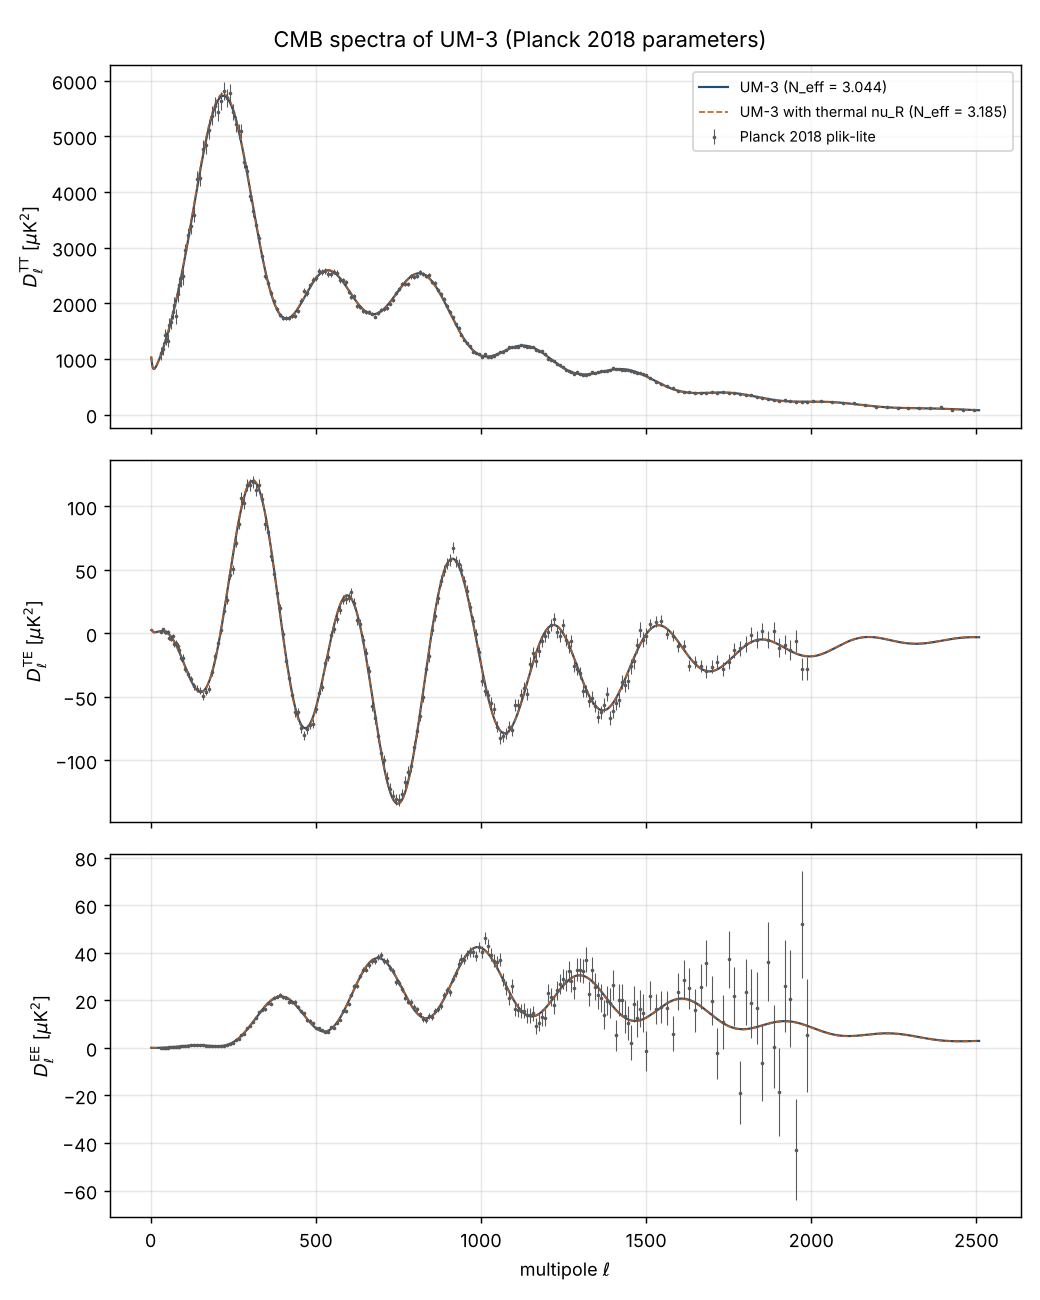
\includegraphics{outputs/cmb_spectra.png}
\caption{The CMB spectra of UM-3 with the Planck 2018 parameters
(\(D_l = l(l + 1)C_l/(2\pi)\) of the temperature, the cross-correlation
and the E-mode polarisation, lensed), with three thermal right-handed
neutrinos (dashed), and the Planck 2018 plik-lite data.}
\end{figure}

\hypertarget{the-bao}{%
\subsection{The BAO}\label{the-bao}}

\begin{longtable}[]{@{}
  >{\raggedright\arraybackslash}p{(\columnwidth - 8\tabcolsep) * \real{0.2000}}
  >{\raggedright\arraybackslash}p{(\columnwidth - 8\tabcolsep) * \real{0.2000}}
  >{\raggedright\arraybackslash}p{(\columnwidth - 8\tabcolsep) * \real{0.2000}}
  >{\raggedright\arraybackslash}p{(\columnwidth - 8\tabcolsep) * \real{0.2000}}
  >{\raggedright\arraybackslash}p{(\columnwidth - 8\tabcolsep) * \real{0.2000}}@{}}
\toprule\noalign{}
\begin{minipage}[b]{\linewidth}\raggedright
tracer
\end{minipage} & \begin{minipage}[b]{\linewidth}\raggedright
\(\mathsf{z}\)
\end{minipage} & \begin{minipage}[b]{\linewidth}\raggedright
measured (DESI DR2)
\end{minipage} & \begin{minipage}[b]{\linewidth}\raggedright
UM-3
\end{minipage} & \begin{minipage}[b]{\linewidth}\raggedright
\(\chi^2\)
\end{minipage} \\
\midrule\noalign{}
\endhead
\bottomrule\noalign{}
\endlastfoot
BGS & 0.295 & \(D_{\mathrm{V}}/r_{\mathrm{s}} = 7.942 \pm 0.075\) &
8.057 & 2.34 \\
LRG1 & 0.510 & \(D_{\mathrm{M}}/r_{\mathrm{s}} = 13.588 \pm 0.167\),
\(D_{\mathrm{H}}/r_{\mathrm{s}} = 21.863 \pm 0.425\) & 13.500, 22.739 &
4.48 \\
LRG2 & 0.706 & \(17.351 \pm 0.177\), \(19.455 \pm 0.330\) & 17.700,
20.169 & 14.36 \\
LRG3+ELG1 & 0.934 & \(21.576 \pm 0.152\), \(17.641 \pm 0.193\) & 21.994,
17.569 & 8.29 \\
ELG2 & 1.321 & \(27.601 \pm 0.318\), \(14.176 \pm 0.221\) & 28.081,
14.065 & 2.31 \\
QSO & 1.484 & \(30.512 \pm 0.760\), \(12.817 \pm 0.516\) & 30.275,
12.880 & 0.10 \\
Ly\(\alpha\) & 2.330 & \(38.988 \pm 0.531\), \(8.632 \pm 0.101\) &
39.182, 8.616 & 0.13 \\
\end{longtable}

The BAO distances of UM-3 with the Planck parameters
(\(\Omega_{\mathrm{m}} = 0.3152\), \(h_{100}r_{\mathrm{s}} = 99.09\)
Mpc) against DESI DR2 (DESI Collaboration 2025, Table IV; \(\chi^2\)
with the correlation of \(D_{\mathrm{M}}\) and \(D_{\mathrm{H}}\) of
each tracer): \(\chi^2 = 32.0\) for 13 measurements. Fitted to DESI
alone, \(\Omega_{\mathrm{m}} = 0.2971\) and
\(h_{100}r_{\mathrm{s}} = 101.56\) Mpc with \(\chi^2 = 10.5\) for 11
degrees of freedom (\(p = 0.48\)), as DESI finds for the
cosmological-constant model; the Planck point lies
\(\Delta\chi^2 = 21.5\) above this optimum when its own errors are
neglected (with the CMB errors DESI quotes a 2.3 standard-deviation
tension between BAO and CMB). The dark energy of UM-3 is a vacuum energy
with \(w = -1\) to order \(\epsilon_{\mathrm{r}}\): UM-3 inherits this
tension and cannot produce the evolving dark energy (\(w_0 > -1\),
\(w_a < 0\)) that DESI DR2 with the CMB prefers at 3.1 standard
deviations. Status: DERIVED (C5).

\hypertarget{the-cnb}{%
\subsection{The CNB}\label{the-cnb}}

\[
\Gamma_{\mathrm{C\nu B}} = N_{\mathrm{T}}\,\bar\sigma_{\mathrm{T}}\,\frac{n_\nu^{(0)}}{2}\sum_{i=1}^{3}\lvert U_{\mathrm{e}i}\rvert^2\big(1 + \mathsf{s}_i\big)\qquad(\text{Dirac neutrinos}) \tag{S-23}
\] \textbf{Symbols in (S-23).}

\begin{itemize}
\tightlist
\item
  \(\Gamma_{\mathrm{C\nu B}}\): The rate at which a tritium target
  captures neutrinos of the cosmic neutrino background. Unit: 1/time.
  Status: STANDARD.
\item
  \(N_{\mathrm{T}}\): The number of tritium nuclei of the target. Unit:
  dimensionless. Value: \(2.0\times10^{25}\) for 100 g. Status:
  STANDARD.
\item
  \(\bar\sigma_{\mathrm{T}}\): The averaged cross-section of the capture
  of a non-relativistic electron neutrino on tritium, times the speed of
  light. Unit: cm\(^2\). Value: \(3.834\times10^{-45}\) cm\(^2\).
  Status: STANDARD.
\item
  \(n_\nu\): The number density of the cosmic neutrino background per
  flavour (neutrinos plus antineutrinos, one helicity each);
  \(n_\nu^{(0)}\) its value today. Unit: GeV\(^3\). Value: 112
  cm\(^{-3}\) today. Status: STANDARD.
\item
  \(i\): A generation index (\(i = 1, 2, 3\)), which also labels the
  neutrino mass states \(\nu_1, \nu_2, \nu_3\); a repeated index is not
  summed unless a sum sign is written. Status: STANDARD.
\item
  \(U_{\mathrm{e}i}\): The electron row of the mixing matrix,
  \(U_{\mathrm{e}i} = (U_{\mathrm{PMNS}})_{ei}\):
  \(\lvert U_{\mathrm{e}i}\rvert^2\) is the electron-flavour fraction of
  the mass state \(i\). Unit: dimensionless. Value:
  \(\lvert U_{\mathrm{e}i}\rvert^2 = 0.681, 0.296, 0.022\). Status:
  STANDARD.
\item
  \(\mathsf{s}_i\): The speed of the neutrino mass state \(i\) today (0
  for a non-relativistic state, 1 for a massless one). Unit:
  dimensionless. Status: STANDARD.
\end{itemize}

The capture rate of the cosmic neutrinos on a target of
\(N_{\mathrm{T}}\) tritium nuclei
(\(\nu_e + {}^3\mathrm{H} \to {}^3\mathrm{He} + e^-\), the PTOLEMY
idea): each mass state \(i\) contributes with its electron fraction
\(\lvert U_{\mathrm{e}i}\rvert^2\); for Dirac neutrinos only the
left-handed helicity of each state is populated (\(n_\nu^{(0)}/2 = 56\)
cm\(^{-3}\) per state), and it is captured with the averaged
cross-section \(\bar\sigma_{\mathrm{T}} = 3.834\times10^{-45}\) cm\(^2\)
times \((1 + \mathsf{s}_i)\), \(\mathsf{s}_i\) the speed of the state
(Long, Lunardini and Sabancilar 2014). Status: STANDARD.

The CNB of UM-3: the temperature
\(\mathsf{T}_\nu^{(0)} = (4/11)^{1/3}\mathsf{T}_\gamma^{(0)} = 1.9454\)
K (\(1.676\times10^{-4}\) eV); 112.0 neutrinos and antineutrinos per
cm\(^3\) per flavour, 336 in all (FE-53); the states \(\nu_2\) and
\(\nu_3\) became non-relativistic at \(\mathsf{z} = 15.3\) and 94 (where
their mass equals the mean momentum \(3.15\mathsf{T}_\nu\)), \(\nu_1\)
is massless; \(\Omega_\nu h_{100}^2 = 6.31\times10^{-4}\) for the two
massive states (FE-58: \(\sum m_i/93.14\) eV \(= 6.30\times10^{-4}\);
CAMB: \(6.31\times10^{-4}\)). Because the right-handed states are not
populated, the CNB of UM-3 has one helicity per state: a 100 g tritium
target captures 4.1 cosmic neutrinos per year if all states are
non-relativistic (Majorana neutrinos: 8.1, twice as many; Long,
Lunardini and Sabancilar: about 4 and 8), and 6.8 per year with the
massless \(\nu_1\) of UM-3, whose left-handed helicity is captured twice
as often (these captures lie at the end point of the beta spectrum,
where only a mass of \(\nu_1\) would separate them). The sum of the
masses, 0.0587 eV, lies below the bounds of DESI DR2 with the CMB (0.064
eV) and of ACT DR6 (0.082 eV, 95\%). Status: DERIVED (C6).

\hypertarget{what-the-solution-does-not-settle}{%
\section{What the solution does not
settle}\label{what-the-solution-does-not-settle}}

\begin{itemize}
\tightlist
\item
  \textbf{The media of the bulk} (ASSUMED). The late universe needs a
  medium in the bulk that keeps the bulk static (the stabiliser) and,
  with frozen extra times, a medium of the frozen branch; both violate
  the null energy condition (S-3), so no ordinary field provides them,
  and UM-3 gives no field theory for them. The power series additionally
  needs the medium to respond to the matter of the fold with the radion
  mode (S-8, S-9); a rigid medium would change the expansion law in a
  way that observation excludes.
\item
  \textbf{The primordial era} (OPEN). The author's vacuum is degenerate
  (S-1: the linear response of the bulk equations vanishes, and the
  transverse traceless graviton has no time-kinetic term there); a
  varying \(b_4\) needs bulk sources of second order in its rate (S-2);
  the passage from the author's vacuum to the static block with frozen
  extra times is not computed, and the primordial spectrum, the optical
  depth and the densities are taken from Planck 2018.
\item
  \textbf{The Krein norm} (OPEN). The charge of dirac16complex is
  indefinite (FE-43): of the eight bound states at
  \(+\omega_{\mathrm{b}}\) four carry positive and four negative energy.
  The Kohn-Sham states occupy the four of positive energy, without the
  negative-energy sea; whether the quantised theory with both kinds of
  states is stable is not settled.
\item
  \textbf{The extra times} (ASSUMED, OPEN). Every field that depends on
  the extra times is tachyonic (FE-38); UM-3 keeps only fields that do
  not depend on them, and the stability of the theory without this
  restriction is open.
\item
  \textbf{Lorentz violation in the bulk} (DERIVED). Zero modes of bulk
  fields and the bound particles \(\chi\) move faster than light on the
  fold (S-12, S-13). For the Standard Model this fixes its place on the
  fold; for \(\chi\) it requires \(q_{\mathrm{b}} > H\) and, with the
  direct-detection bound
  \(q_{\mathrm{b}} \lesssim 0.03\,\omega_{\mathrm{b}}\), a bulk scale
  \(H\) well below the mass of \(\chi\).
\item
  \textbf{The dark energy} (ASSUMED). The vacuum energy \(\rho_\Lambda\)
  of the fold is a free parameter: UM-3 accommodates its value but does
  not explain it, and it has \(w = -1\), so the evolving dark energy
  that DESI DR2 with the CMB prefers is not available.
\item
  \textbf{The free parameters}. The bulk mass \(m_\Psi\), the scale
  \(H\), the portal couplings, the self-coupling \(\lambda_\Psi\), the
  amplitude \(v_{\mathcal{A}}\) and rate \(a_{40}\) of the ad hoc
  vacuum, the lightest neutrino mass (taken as zero) are not fixed by
  UM-3; the relic density fixes one combination of the mass of \(\chi\)
  and its portals.
\item
  \textbf{Neutrinos in dense matter} (STANDARD, ESTIMATE). The
  non-linear evolution of the fast instability and the collective
  conversion deep in a supernova are not solved; their outcome is
  modelled by the equipartition FE-52, whose effect on the explosion is
  taken from the transport simulations of Gogilashvili and Tamborra.
\end{itemize}

\hypertarget{what-was-verified}{%
\section{What was verified}\label{what-was-verified}}

Every result labelled DERIVED rests on a computation in the folder
\texttt{universe\_model\_3/code/} of the repository, which checks itself
and writes a report to \texttt{universe\_model\_3/reports/} (all
equations and results are written out above). Each script is run with
\texttt{python\ universe\_model\_3/code/NAME.py} (Python 3 with numpy,
scipy, sympy, matplotlib and CAMB 2.0.5; the cosmology script downloads
the Planck 2018 plik-lite files from
github.com/heatherprince/planck-lite-py into
\texttt{universe\_model\_3/external/} once).

\begin{itemize}
\tightlist
\item
  \texttt{um3\_dirac\_matrices.py} (55 checks): the author's matrices,
  their reality, the Clifford relations, the chiral projectors,
  Pin(4,4).
\item
  \texttt{um3\_geometry.py} (26 checks): the exact curvature of the
  author's metric, the Lovelock tensors by two routes, the trace and
  Bianchi identities, the background equations FE-29, the author's
  vacuum and its degeneracy, the spin connection and the vielbein
  postulate.
\item
  \texttt{um3\_fold.py} (13 checks): the proper chart, the general
  warped metric FE-34, the junction potential, the fold sources, the
  conservation law at the fold.
\item
  \texttt{um3\_bulk.py} (10 checks): the zero modes and the speeds of
  bulk scalars, photons, fermions and gravitons (S-11, S-12).
\item
  \texttt{um3\_fields.py} (16 checks): the bilinears of dirac16complex,
  the Krein operator, the electroweak masses of the ad hoc vacuum, the
  anomalies with three right-handed neutrinos.
\item
  \texttt{um3\_spectra.py} (5 checks): the bound states FE-40 with the
  exact \(16 \times 16\) matrices, their Krein signature, their speed
  (S-13).
\item
  \texttt{um3\_background.py} (6 checks): S-1 to S-4, the ad hoc vacuum
  as a gauge rotation and its residual (S-10).
\item
  \texttt{um3\_series.py} (6 checks): S-5 to S-9.
\item
  \texttt{um3\_kohnsham.py} (KS\_NCHECKS checks): the Kohn-Sham states
  (S-24 to S-28) in three regimes, lifted to sixteen components.
\item
  \texttt{um3\_neutrino.py} (5 checks): the flavour blindness of
  \(V_\Psi\), the resonance formulas, the crossing criterion, the
  equipartition, the CNB numbers.
\item
  \texttt{um3\_flavour.py} (4 checks): S-14 to S-17.
\item
  \texttt{um3\_thermal.py} (6 checks): the degrees of freedom, S-18 to
  S-20, the ad hoc vacuum before nucleosynthesis.
\item
  \texttt{um3\_cosmology.py} (6 checks): S-21 to S-23 and the
  comparisons with Planck 2018 and DESI DR2.
\end{itemize}

\end{document}
